
\documentclass[acronym,symbols]{fei}

%\pagestyle{headings}

\usepackage[utf8]{inputenc}
\usepackage[english]{babel}
\usepackage{amsmath}
\usepackage{amssymb}
\usepackage{array}
\usepackage{colortbl}
\usepackage{makecell}
\usepackage{longtable}


%\usepackage{afterpage}
%\usepackage{amsfonts}
%\usepackage{comment}
%\usepackage{csquotes}
%\usepackage{easytable}
%\usepackage{here}
%\usepackage{indentfirst}
%\usepackage{lipsum}
%\usepackage{listings}
%\usepackage{longtable}
%\usepackage{multicol}
%\usepackage{multirow}
%\usepackage{microtype}
%\usepackage{pdflscape}
%\usepackage{pgfgantt}
%\usepackage{setspace}
%\usepackage{stmaryrd}
%\usepackage{tabularx}
%\usepackage{tikz}
%\usepackage{url}


%%%%%%%%%%%%%%%%%%%%%%%%%%%%%%%%%%%%%%%%%%%%%%%%%%%%%%%%%%%%%%%%%%%%%%%%%%%%%%%%%%%%%%%%%%%%%%%%%%%%%%%%
%%%% -- Configuracoes Iniciais
%%%%%%%%%%%%%%%%%%%%%%%%%%%%%%%%%%%%%%%%%%%%%%%%%%%%%%%%%%%%%%%%%%%%%%%%%%%%%%%%%%%%%%%%%%%%%%%%%%%%%%%%

\author{André Luiz Florentino}
%\cidade{Cidade}
%\instituicao{Instituição de Ensino}
\title{ENVIRONMENTAL SOUND RECOGNITION IN EMBEDDED SYSTEMS FOR AUTONOMOUS VEHICLES}

% comando para inserção de subfloats do tipo figure, usado aqui no template
% remova este comando se for usar o pacote subfig
% não recomendo o pacote subcaption

%\newsubfloat{figure}

%\subtitulo{subtítulo}

%%%%%%%%%%%%%%%%%%%%%%%%%%%%%%%%%%%%%%%%%%%%%%%%%%%%%%%%%%%%%%%%%%%%%%%%%%%%%%%%%%%%%%%%%%%%%%%%%%%%%%%%
%%%% -- Entradas Listas de Abreviaturas e Simbolos
%%%%%%%%%%%%%%%%%%%%%%%%%%%%%%%%%%%%%%%%%%%%%%%%%%%%%%%%%%%%%%%%%%%%%%%%%%%%%%%%%%%%%%%%%%%%%%%%%%%%%%%%

%%%%%%%%%%%%%%%%%%%%%%%%%%%%%%%%%%%%%%%%%%%%%%%%%%%%%%%%%%%%%%%%%%%%%%%%%%%%%%%%%%%%%%%%%%%%%%%%%%%%%%%%
%%%% -- Entradas Listas de Abreviaturas e Simbolos
%%%%%%%%%%%%%%%%%%%%%%%%%%%%%%%%%%%%%%%%%%%%%%%%%%%%%%%%%%%%%%%%%%%%%%%%%%%%%%%%%%%%%%%%%%%%%%%%%%%%%%%%

%%% units and symbols

\newglossaryentry{hz}{type=symbols,name={\text{Hz}},sort=hz,description={Hertz}}
\newglossaryentry{db}{type=symbols,name={\text{dB}},sort=db,description={Decibel}}
\newglossaryentry{b}{type=symbols,name={\text{B}},sort=b,description={Byte}}
\newglossaryentry{s}{type=symbols,name={\text{s}},sort=s,description={Second}}
\newglossaryentry{mi}{type=symbols,name={\text{m}},sort=mi,description={Mili, $10^{-3}$}}
\newglossaryentry{k}{type=symbols,name={\text{k}},sort=k,description={Kilo, $10^3$}}
\newglossaryentry{m}{type=symbols,name={\text{M}},sort=me,description={Mega, $10^6$}}
\newglossaryentry{g}{type=symbols,name={\text{G}},sort=g,description={Giga, $10^9$}}


%%% Entities

\newacronym[longplural=Preferred Reporting Items for Systematic Reviews]{prisma}{PRISMA}{Preferred Reporting Items for Systematic Reviews}
\newacronym[longplural=Society of Automotive Engineers]{sae}{SAE}{Society of Automotive Engineers}
\newacronym[longplural=Detection and Classification of Acoustic Scenes and Events]{dcase}{DCASE}{Detection and Classification of Acoustic Scenes and Events}


%%% General Concepts
\newacronym[longplural=Field-Programmable Gate Arrays]{fpga}{FPGA}{Field-Programmable Gate Arrays}
\newacronym[longplural=Tensor Processing Units]{tpu}{TPU}{Tensor Processing Units}
\newacronym[longplural=Graphics Processing Unit]{gpu}{GPU}{Graphics Processing Unit}
\newacronym[longplural=Application Programming Interface]{api}{API}{Application Programming Interface}
\newacronym[longplural=Environmental Sound Recognition]{esr}{ESR}{Environmental Sound Recognition}
\newacronym[longplural=Radio Detection And Ranging]{radar}{RADAR}{Radio Detection And Ranging}
\newacronym[longplural=Light Detection and Ranging]{lidar}{LiDAR}{Light Detection and Ranging}
\newacronym[longplural=Short Time Fourier Transform]{stft}{STFT}{Short Time Fourier Transform}
\newacronym[longplural=Fast Fourier Transform]{fft}{FFT}{Fast Fourier Transform}
\newacronym[longplural=Discrete Fourier Transform]{dft}{DFT}{Discrete Fourier Transform}
\newacronym[longplural=Discrete Cosine Transform]{dct}{DCT}{Discrete Cosine Transform}
\newacronym[longplural=Random Access Memory]{ram}{RAM}{Random Access Memory}
\newacronym[longplural=standard deviation]{std}{std}{standard deviation}
\newacronym[longplural=Human-Computer Interaction]{hci}{HCI}{Human-Computer Interaction}
\newacronym[longplural=Electrics \& Electronics]{ee}{EE}{Electrics \& Electronics}
\newacronym[longplural=Sound Pressure Level]{spl}{SPL}{Sound Pressure Level}
\newacronym[longplural=Speech Intelligibility]{si}{SI}{Speech Intelligibility}
\newacronym[longplural=Frequency Response]{fr}{FR}{Frequency Response}
\newacronym[longplural=Active Noise Control]{anc}{ANC}{Active Noise Control}
\newacronym[longplural=Electret Condenser]{ecm}{ECM}{Electret Condenser}
\newacronym[longplural=Microelectromechanical Systems]{mems}{MEMS}{Microelectromechanical Systems}


%%% Specific Concepts
\newacronym[longplural=[Root Mean Square]{rms}{RMS}{Root Mean Square}
\newacronym[longplural=[Zero-Crossing Rate]{zcr}{ZCR}{Zero-Crossing Rate}
\newacronym[longplural=[Mel-Frequency Cepstral Coefficients]{mfcc}{MFCC}{Mel-Frequency Cepstral Coefficients}
\newacronym[longplural=[Spectral Centroid]{sc}{SC}{Spectral Centroid}
\newacronym[longplural=[Spectral Bandwidth]{sb}{SB}{Spectral Bandwidth}
\newacronym[longplural=[Spectral Contrast]{sct}{SCT}{Spectral Contrast}
\newacronym[longplural=[Spectral Roll-off Frequency]{srp}{SRP}{Spectral Roll-off Point}
\newacronym[longplural=[Standard Frame Based]{sfb}{SFb}{Standard Frame Based}
\newacronym[longplural=[Standard Temporal Integration]{sti}{STi}{Standard Temporal Integration}
\newacronym[longplural=[Standard Temporal Integration]{eti}{ETi}{Standard Temporal Integration}
\newacronym[longplural=[Mean Sequential Difference]{msd}{MSD}{Mean Sequential Difference}
\newacronym[longplural=[Mean Crossing Rate]{mcr}{MCR}{Mean Crossing Rate}
\newacronym[longplural=[Flatness]{fla}{FLA}{Flatness}
\newacronym[longplural=[Crest Factor]{crf}{CRF}{Crest Factor}
\newacronym[longplural=[Linear Predictive Cepstral Coefficients]{lpcc}{LPCC}{Linear Predictive Cepstral Coefficients}
\newacronym[longplural=[Computational Auditory Scene Analysis]{casa}{CASA}{Computational Auditory Scene Analysis}
\newacronym[longplural=[UrbanSound8K]{us8k}{US8K}{UrbanSound8K}
\newacronym[longplural=[Direction-of-Arrival]{doa}{DoA}{Direction-of-Arrival}
\newacronym[longplural=[Analog-to-Digital Conversion]{adc}{ADC}{Analog-to-Digital Conversion}
\newacronym[longplural=[Digital-to-Analog Conversion]{dac}{DAC}{Digital-to-Analog Conversion}
\newacronym[longplural=[Pulse-Code Modulation]{pcm}{PCM}{Pulse-Code Modulation}
\newacronym[longplural=[Attack-Decay-Sustain-Release]{adsr}{ADSR}{Attack-Decay-Sustain-Release}


%%%% Machine Learning - Networks
\newacronym[longplural=[k-Nearest Neighbors]{k-nn}{k-NN}{k-Nearest Neighbors}
\newacronym[longplural=[Support Vector Machine]{svm}{SVM}{Support Vector Machine}
\newacronym[longplural=[Radial Basis Function]{rbf}{RBF}{Radial Basis Function}
\newacronym[longplural=[Artificial Neural Network]{ann}{ANN}{Artificial Neural Network}
\newacronym[longplural=[Multilayer Perceptron]{mlp}{MLP}{Multilayer Perceptron}
\newacronym[longplural=[Convolutional Neural Network]{cnn}{CNN}{Convolutional Neural Network}
\newacronym[longplural=[Long Short-Term Memory]{lstm}{LSTM}{Long Short-Term Memory}
\newacronym[longplural=[Generative Adversarial Network]{gan}{GAN}{Generative Adversarial Network}
\newacronym[longplural=[Logistic Regression]{lr}{LR}{Logistic Regression}
\newacronym[longplural=[Gaussian Naïve Bayes]{gnb}{GNB}{Gaussian Naïve Bayes}
\newacronym[longplural=[Generalized Linear Model]{glm}{GLM}{Generalized Linear Model}
\newacronym[longplural=[Gaussian Mixture Model]{gmm}{GMM}{Gaussian Mixture Model}
\newacronym[longplural=[Yet another Audio Mobilenet Network]{yamnet}{YAMNet}{Yet another Audio Mobilenet}
\newacronym[longplural=[Principal Component Analysis]{pca}{PCA}{Principal Component Analysis}
\newacronym[longplural=[Stochastic Gradient Descent]{sgd}{SGD}{Stochastic Gradient Descent}
\newacronym[longplural=[Rectified Linear Unit]{relu}{ReLU}{Rectified Linear Unit}


%%%% Hardware
\newacronym[longplural=[Electronic Control Unit]{ecu}{ECU}{Electronic Control Unit}
\newacronym[longplural=[Vehicle Control Unit]{vcu}{VCU}{Vehicle Control Unit}
\newacronym[longplural=[Controller Area Network]{can}{CAN}{Controller Area Network}
\newacronym[longplural=[System on Chip]{soc}{SoC}{System on Chip}



% Syncronized references with Zotero
\addbibresource{resources/bibliography/zotero.bib}

% Manually reworked reference file from Zotero to match ABNT latest requirements
% \addbibresource{resources/bibliography/zotero_manual.bib}

\makeglossaries

\begin{document}

\maketitle

\selectlanguage{english}

\begin{folhaderosto}
Master's thesis, presented to the University Center of FEI for the purpose of obtaining the degree of Master of Science (MS.c) in Electrical Engineering. Main advisor Prof. Dr. Plinio Thomaz Aquino Junior.
\end{folhaderosto}

\fichacatalografica
\folhadeaprovacao

% Quando disponível, substituir as duas linhas acima pelos PDFs carregados no documento.
%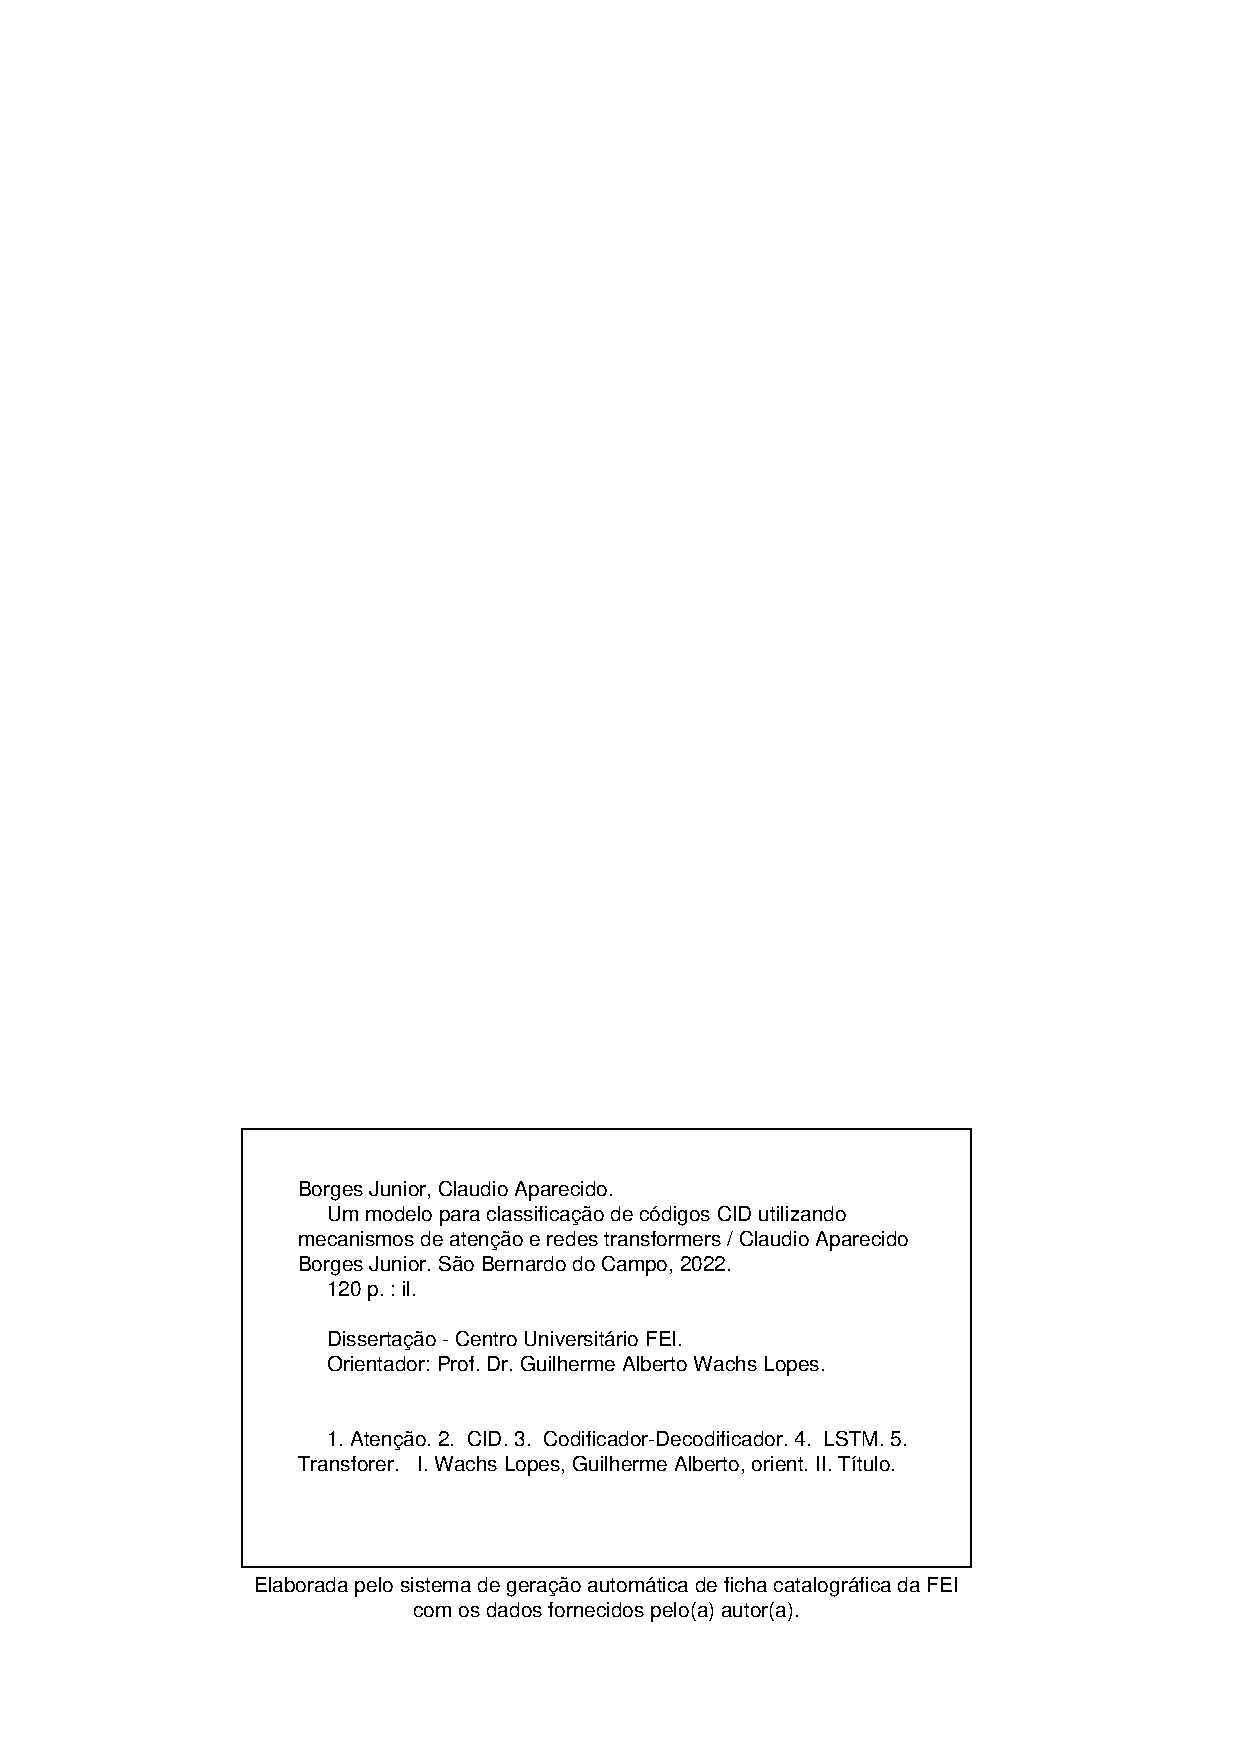
\includepdf{_ficha_catalografica.pdf}

\dedicatoria{I dedicate this study to Almighty God, to my beloved wife Priscila, and in loving memory of my parents who guided me along the path of integrity, choosing what is right over what is easy.}

\begin{agradecimentos}
First and foremost, I would like to express my profound gratitude to God for the gift of life and the resilience provided to navigate challenges.

My heartfelt thanks go to my advisor, Prof. Dr. Plinio Thomaz Aquino Junior, for unwavering support throughout all stages of this study. I am also grateful to my former advisor, Prof. Dr. Guilherme Alberto Wachs Lopes, whose guidance introduced me to essential tools for the completion of this dissertation.

I extend my appreciation to the entire staff at FEI and my work colleagues at EDAG GmbH. Special thanks to Mr. Martin Vollmer and Mr. Alexandre Sberveglieri for their invaluable contributions to my professional development, and to Mr. Johannes Barckmann, Mr. Michael Jahn, and Mr. Maximilan Happel for their support in this project.

Finally, I am deeply indebted to my beloved wife, whose unconditional support served as a constant source of strength during these three years. In moments of discouragement, her presence was my sanctuary, providing me hope and inspiration to continue moving forward.
\end{agradecimentos}

\begin{epigrafe}
	\epig{Our greatest weakness lies in giving up. The most certain way to succeed is always to try just one more time.}{Thomas A. Edison}
	\epig{We don't have better algorithms, we just have more data.}{Peter Norvig}
\end{epigrafe}
\begin{abstract}

\glsunsetall


The autonomous vehicle market is experiencing significant growth, with indications of transitioning from the "trough of disillusionment" to the "slope of enlightenment" on the Gartner hype cycle chart. The fundamental technologies encompassing extensive data analytics, computational capabilities, and sensor fusion techniques have already been established, and all stakeholders in this industry are persistently exploring novel approaches to enhance the overall perception of end users in terms of safety and trustworthiness. In this context, this project aims to develop and implement an Environmental Sound Recognition (ESR) algorithm in an embedded system for deployment in autonomous vehicles for smart cities in 2025, targeting advanced functionalities for early warning systems. Due to the hardware constraints, a regular passenger vehicle was used, embedding the ESR algorithm on a Raspberry Pi with a microphone array. The limited literature on ESR algorithms for vehicles primarily focuses on siren detection without real-time inferences, and to address this, a dataset benchmarking study confirmed classifiers' accuracy, leading to the creation of a new dataset tailored to autonomous vehicles. This new dataset provided a comprehensive baseline where several classifiers were trained and evaluated for their accuracy, memory usage, and prediction time, with CNN 2D using aggregated features emerging as the top-performing model, achieving an average accuracy of 83\% in a single window process and 80\% in sliding window process. During the indoor experiment, the total prediction time achieved an average of 47.6 ms, validating the algorithm’s performance with weighted F1-scores close or better than cross-validation results. In the final phase of the methodology, real-world tests conducted in a passenger vehicle yielded similar results, however, inconsistencies were noted in certain classes due to insufficient sample diversity and environmental noise, which affected their accuracy. The results of this project indicate that its general objective was successfully achieved, contributing to the understanding of ESR algorithms in embedded systems within passenger vehicles and it is ready for integration into the electric \& electronic architecture of autonomous vehicles for smart cities. Additionally, upon conducting further experiments across various vehicle categories to assess cabin insulation effects, this project could potentially enhance safety features for drivers with hearing impairments by adapting the ESR algorithm as an add-on feature in regular passenger vehicles.

\glsresetall

\keywords{Environmental Sound Recognition, Autonomous Vehicle, Embedded System, Aggregated Features, Feature extraction.}
\end{abstract}

\begin{resumo}

O mercado de veículos autônomos vem crescendo significativamente, indicando uma transição do "vale da desilusão" para a "inclinação da iluminação" no gráfico \textit{Gartner hype cycle}. As tecnologias essenciais que abrangem análise extensa de dados, capacidades computacionais avançadas e técnicas de fusão de sensores já foram estabelecidas e as partes interessadas nesta indústria estão constantemente explorando novas abordagens para aprimorar a percepção global dos usuários finais em termos de segurança e confiabilidade. Nesse contexto, este projeto visa desenvolver e implementar um algoritmo de Reconhecimento de Sons Ambientais (ESR) em sistema embarcado para implantação em veículos autônomos para cidades inteligentes em 2025, visando funcionalidades avançadas para sistemas de alerta precoce. Devido às limitações de hardware, foi utilizado um veículo de passageiros comum, incorporando o algoritmo ESR em um Raspberry Pi com uma matriz microfônica. A literatura sobre algoritmos ESR para veículos se concentra na detecção de sirenes sem inferências em tempo real. Para resolver esse problema, um estudo de \textit{benchmarking} de datasets confirmou a precisão dos classificadores, levando à criação de um novo dataset adaptado a veículos autônomos. Este dataset forneceu uma base de referência onde vários classificadores foram treinados e avaliados quanto à sua precisão, uso de memória e tempo de predição, com a CNN 2D usando características agregadas se destacando com o melhor desempenho, alcançando uma precisão média de 83\% em processo de janela única e 80\% em processo de janela deslizante. Um experimento em ambiente interno validou o desempenho do algoritmo com valores de F1-score ponderado próximos ou melhores que os resultados da validação cruzada, com tempo total de predição médio de 47,6 ms. Na fase final da metodologia, testes em ambiente externo com um veículo de passageiros demonstraram resultados semelhantes, embora inconsistências tenham sido observadas em certas classes devido à falta de diversidade das amostras e ao ruído ambiental, penalizando sua precisão. O projeto alcançou com sucesso seu objetivo geral e está pronto para integração na arquitetura elétrica e eletrônica de veículos autônomos para cidades inteligentes. Além disso, ao conduzir experimentos adicionais em várias categorias de veículos para avaliar os efeitos da isolação da cabine, este projeto poderia potencialmente melhorar as características de segurança para motoristas com deficiência auditiva ao adaptar o algoritmo ESR como uma funcionalidade adicional em veículos comuns.

\palavraschave{Reconhecimento de Som Ambiental, Veículo Autônomo, Sistema Embarcado, Características Agregadas, Extração de Características.}
\end{resumo}

\listoffigures
\listoftables
\printglossaries
\tableofcontents

\setcounter{table}{0}

    \chapter{INTRODUCTION}
\label{chp:introduction}

The autonomous vehicle market is experiencing rapid expansion, with numerous established brands and startups dedicating considerable efforts, resources, and investments to secure a position in this lucrative sector that may create 300\$ billion to 400\$ billion in revenues by the year 2035 \cite{McKinsey2023}. These companies strive to offer sustainable, technologically advanced solutions that enhance user experience and provide innovative advancements. In recent years, there has been a proliferation of essential technologies that have greatly facilitated the advancement and reliable operation of autonomous vehicles, including the availability of large-scale data analytics (commonly known as big data), increased computational capabilities, and a wide range of sensor technologies such as ultrasonic sensors, \gls{radar}, \gls{lidar}, cameras, and the integration of all these sensors through sensor fusion techniques \cite{Hussainj2018}.

According to the \gls{sae}, autonomous vehicles can be classified into six levels based on their ability to operate without human intervention. Level 0 represents vehicles that rely entirely on human drivers for all aspects of driving. Level 1 vehicles have certain functions automated, such as braking or steering, but still require full driver engagement. At Level 2, the automation system can control both steering and acceleration/deceleration, while the driver must remain fully attentive and ready to take control when needed. Level 3 vehicles can operate autonomously under certain conditions, allowing the driver to engage in other tasks, but prompt transition is required if the system requests intervention. Level 4 vehicles are highly autonomous and can operate without human input in specific geographic areas or predetermined scenarios, but not in all conditions. Finally, Level 5 vehicles are fully autonomous and can operate under all conditions, without the need for human intervention, enabling passengers to engage in non-driving related activities \cite{SAE2021}.

Much like a human driver relies on their sight, touch, and hearing to navigate and make informed decisions on the road, autonomous vehicles have primarily focused on vision and touch, neglecting the crucial sense of hearing or audition. This omission is akin to a human driver being deprived of their ability to hear, which would severely limit their situational awareness and pose significant challenges in detecting important auditory cues, such as emergency vehicle sirens, approaching vehicles or any other road users.

In the realm of human perception, the ability to effortlessly segregate and identify individual sound sources within a complex acoustic mixture is a common phenomenon, for instance, an individual can effortlessly pick out a specific voice amidst a bustling background that includes the voices of other individuals and music. The field of sound analysis, commonly referred to in the literature as \gls{casa} \cite{Hermes2023}, delves into the investigation of methods to disentangle and recognize sound sources present in an auditory scene with the primary objective to equip computers with the ability to perceive and comprehend audio content, akin to the human auditory system. 

Given the vast scope of \gls{casa} applications, this field of research is typically subdivided into three core areas according to \textcite{Wang2006}:

\begin{itemize}
    \item \textbf{Context awareness}, also known as audio context recognition, pertains to identifying the location or ongoing activity within a specific environment based on audio information or events. It provides a context location of the sound, such as determining whether it's coming from a supermarket or a highway;
    \item \textbf{Sound event detection and recognition} involves categorizing individual sound events present in an auditory scene. It addresses the question of "who and what" by recognizing the specific sound sources within the scene, for example a children crying;
    \item \textbf{General audio classification} involves classifying and recognizing the contents of audio signals, commonly utilized for audio content retrieval, indexing, and audio-based searching.  
\end{itemize}

Understanding the acoustic environment by \textbf{detecting and recognizing sound events} can be crucial for autonomous vehicles to perceive and react to their surroundings, providing a more comprehensive sensory system for safer and more efficient autonomous driving. By deploying audio classification algorithms on embedded systems within these vehicles, real-time \gls{esr} can be achieved, allowing for advanced functionalities such as emergency vehicle detection, sound-based traffic monitoring, and early warning systems. Moreover, the effective utilization of embedded systems can alleviate the burden on external computing infrastructure and facilitate seamless integration of \gls{esr} into the existing vehicle architecture.


There is a substantial body of literature covering \gls{esr} algorithms that are implemented on embedded devices, operating at both low-level platforms such as microcontrollers \cite{Abreha2014} and \cite{Nordby2019}, as well as high-level platforms like \gls{fpga} and \gls{tpu} \cite{Silva2019}, \cite{Vandendriessche2021} and \cite{Lhoest2021}. Despite the lack of research focusing on the application of these algorithms in autonomous vehicles or regular passenger vehicles, there is significant potential for research and development in this area. By addressing this research gap, the overall performance and safety of autonomous and regular passenger vehicles can be improved, while also making valuable contributions to the emerging field of acoustic perception in intelligent transportation systems. In addition to the identified research gap, it is worth noting that the field of acoustic perception in intelligent transportation systems has already attracted attention in the industry. Google Inc., for instance, has filed a patent related to the utilization of audio data for controlling autonomous vehicles \cite{Ferguson2014}.


\section{CONTEXT}
\label{sec:introduction_context}

Urban mobility is a complex interaction of energy usage, movement patterns, and spatial allocation, and particularly in densely populated cities, space is a scarce and highly valuable resource. The extent and design of available space determine individuals' abilities to accomplish their professional and personal objectives, reconcile their desires and necessities, and enhance the quality of their living and working conditions. An alternative to achieving these goals relies on urban centers being planned with reduced vehicle presence, decreased parking infrastructure, and minimized environmental pollution. Furthermore, the integration of previously distinct and individual mobility systems is necessary to create a cohesive and efficient urban mobility network.

The concept of "Smart City" has emerged as a response to the global phenomenon of urbanization and the projected growth of cities. This overarching term, embraced by politics, business, administration, and urban planning, encapsulates comprehensive development strategies aimed at enhancing efficiency, technological advancement, sustainability, and inclusivity within cities, primarily concentrate on technical, economic, and social innovations \cite{EDAG2020}.

To fulfill the objectives of Smart City endeavors, certain technical and urban planning prerequisites need to be addressed, namely a few of them:

\begin{itemize}
    \item Establishing designated areas for new mobility concepts where only bicycles are allowed, prohibiting individual or private vehicles. Pedestrians should always have priority over other vehicles, and designated pedestrian crossings may not be necessary;
    \item Integrating public transportation into the urban mobility system;
    \item Adhering to open data and open standards, as well as promoting interoperability and barrier-free principles;
    \item Incorporating Park+Ride zones on the outskirts of the city into the mobility system;
    \item Expanding the network of cycling paths in newly available areas;
    \item Ensuring that \textbf{autonomous transport systems} are constantly active, equipped with self-learning capabilities, intelligent decision-making algorithms, and future-oriented designs;
    \item Implementing appropriate software solutions for traffic control and coordination, potentially eliminating the need for traditional traffic lights;
    \item Collaborating with municipalities, industry stakeholders, and civil society to develop and expand these concepts.
\end{itemize}

One critical component of Smart Cities will be the implementation of the autonomous transport systems, named hereinafter as C-Bots, swarm-intelligent, multi-functional, and fully autonomous robotic vehicles. These vehicles rely on emissions-free energy derived from fuel cells and possess modular and adaptable features, enabling constant usage throughout the day. Moreover, C-Bots can be equipped with rudimentary tools integrated into their "mover" component and can be fitted with additional modules to serve as passenger carriers, cargo transporters, or city cleaning devices, depending on specific requirements. Figure \ref{fig:introduction_C-Bot_ecosystem} illustrates the proposed ecosystem of the C-Bots under development by the company EDAG Engineering GmbH since 2019.

\begin{figure}[htbp]
    \raggedright
        \caption{Illustration of the C-Bot ecosystem concept.}
        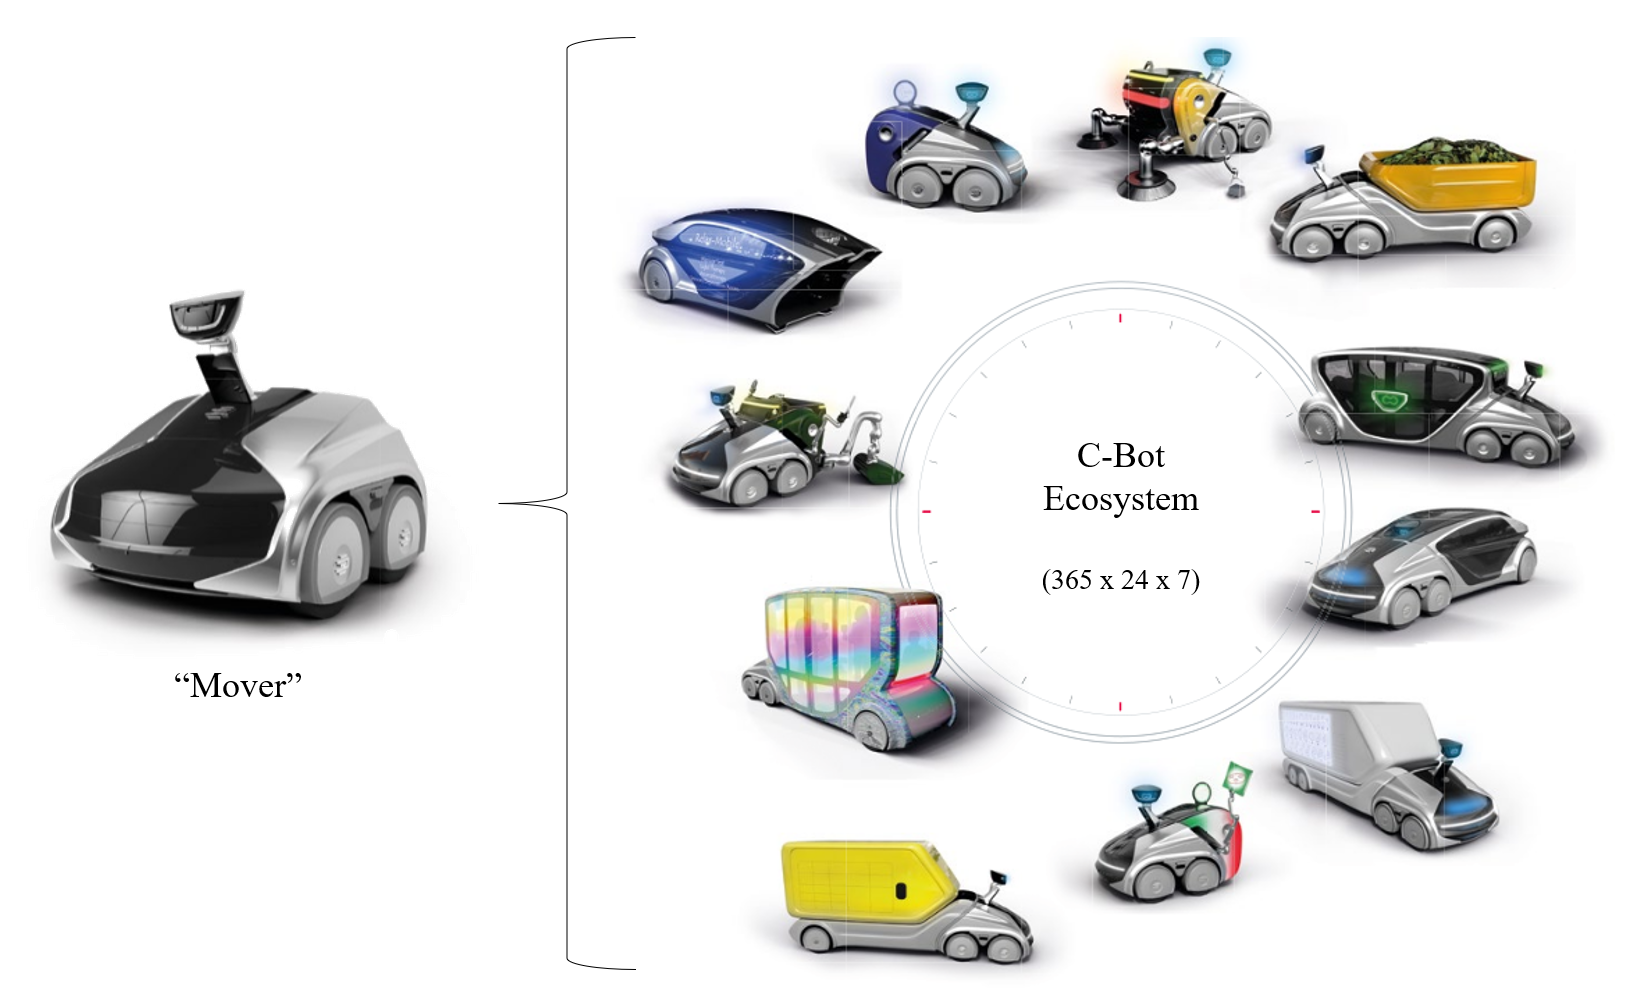
\includegraphics[width=1\textwidth]{resources/images/020-introduction/Introduction_context_C-Bot.png}
        \smallcaption{Source: Author, "adapted from" \textcite{EDAG2020}}
        \label{fig:introduction_C-Bot_ecosystem}
\end{figure} 

In the background, and as part of the C-Bot project, the control system optimizes route planning and the utilization of the C-Bots in continuous 24-hour operation. Users can conveniently input their requests into the system, whether it be the user requesting transportation to the next stop via app, the store owner planning the delivery of new products for the following day, or the municipal vehicle organizing overnight waste removal. This can massively reduce the number of vehicles in city centers, make parking spots available for other uses, and alleviate traffic jams through consistent coordination. All of this makes a significant contribution to the concept of "shared space" traffic, where all \textbf{road users coexist on an equal footing}, and to a smart, sustainable, and livable city.

The project is currently in its third phase, as shown in Figure \ref{fig:introduction_C-Bot_roadmap}, where development partners will explore challenges and possible solutions for core elements of the planned ecosystem: \textbf{automated driving functions}, networking and data exchange, \gls{hci}, \textbf{acceptance and trust}, integrated order management, identification and realization of potential economic and technical optimization in operation, and many more secondary elements \cite{EDAG2020}. 

\begin{figure}[htbp]
    \raggedright
        \caption{Roadmap of the C-Bot development, since its original concept presented in 2019 until its fully implementation in public areas in 2030.}
        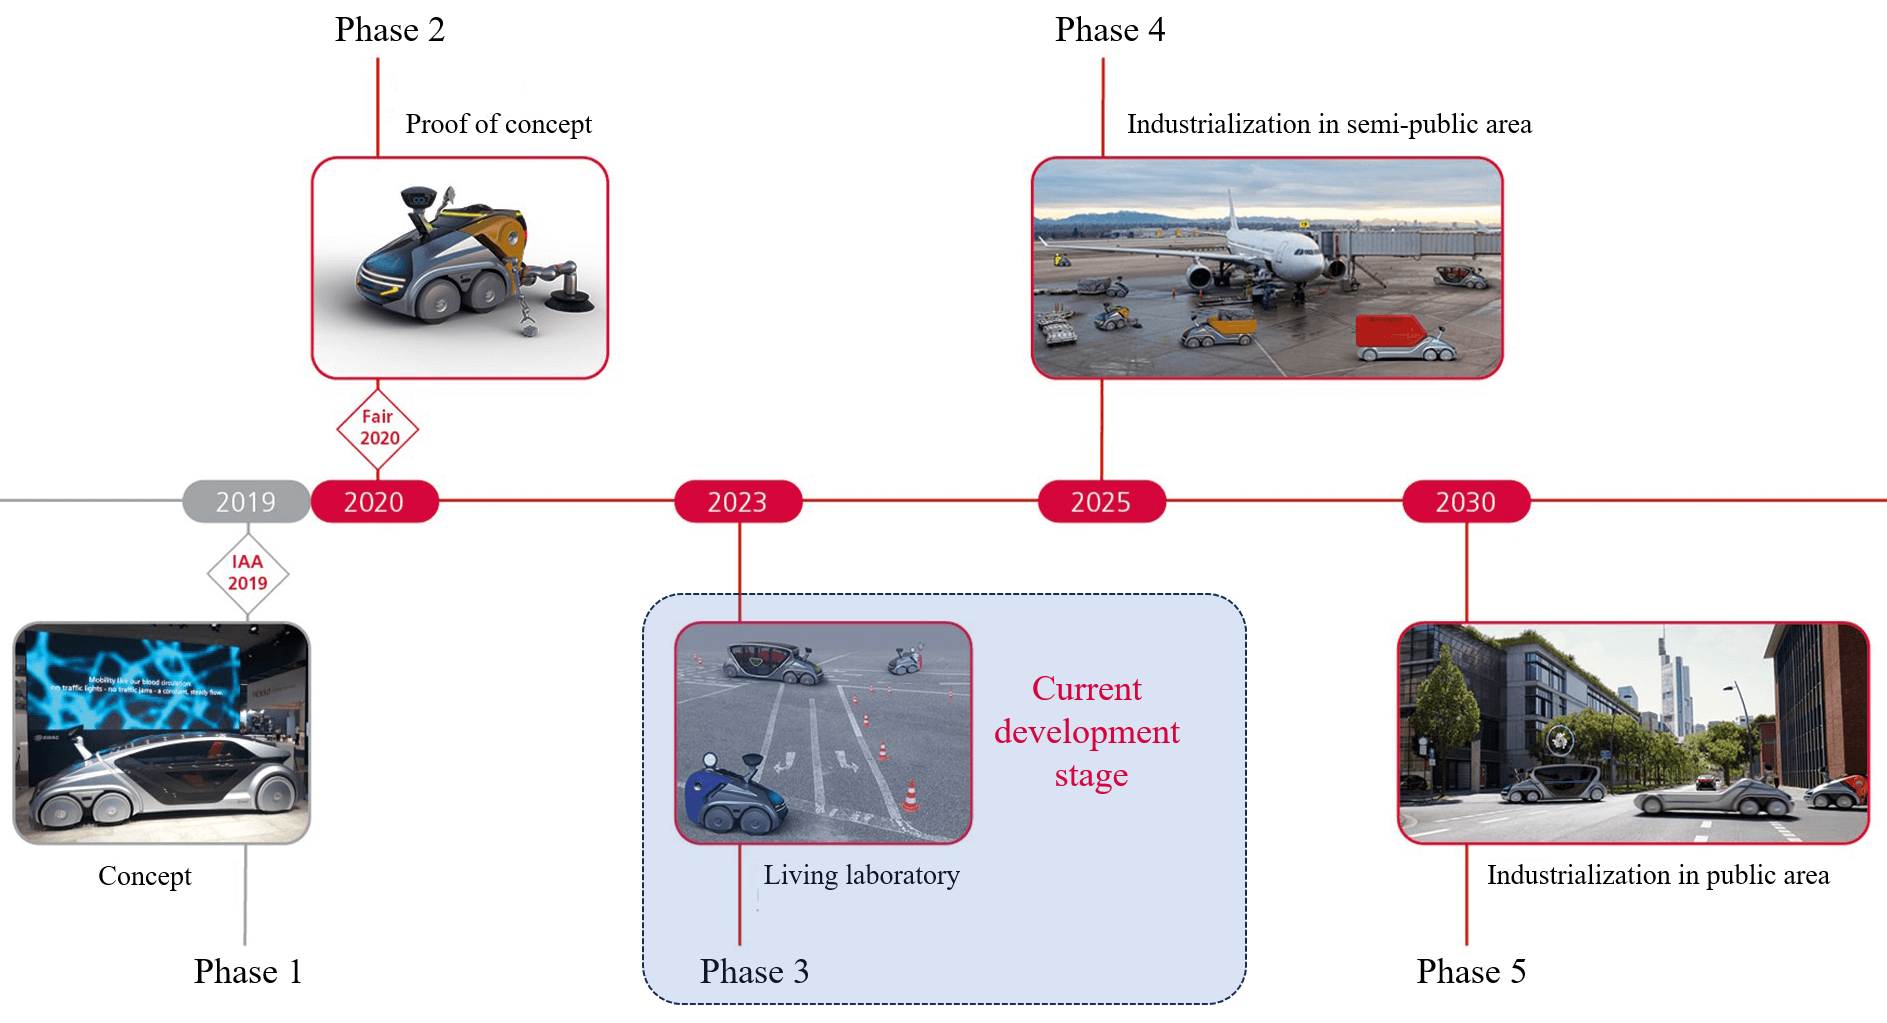
\includegraphics[width=1\textwidth]{resources/images/020-introduction/Introduction_context_C-Bot_roadmap.png}
        \smallcaption{Source: Author, "adapted from" \textcite{EDAG2020}}
        \label{fig:introduction_C-Bot_roadmap}
\end{figure} 

In this phase, the C-Bots are equipped with speech recognition capabilities enabling \gls{hci} with the end-users, however, as in all other autonomous vehicles identified until this publication, \gls{esr} is not yet implemented. Throughout several meetings with the project product owner and the technical staff, the feature of the \gls{esr} was ranked as "important" in the product backlog and it shall be integrated in the next milestone (Phase 4), primarily to confirm its implementation feasibility in the vehicle \gls{ee} and its relevance as a feature itself.


\section{OBJECTIVE}
\label{sec:introduction_objective}

The objective of this study is to develop and implement an \gls{esr} algorithm in embedded systems to be deployed in the C-Bot when the project reaches its next milestone in 2025 (Phase 4). This can be achieved by investigating existing sound recognition algorithms, analyzing their performance, and selecting the most suitable ones for real-time embedded implementation.


\subsection{Specific objectives}
\label{subsec:objectives_specifics}

Considering the context presented in section \ref{sec:introduction_context}, and the fact that the C-Bot hardware construction is under development in a foreign country, an alternative approach to validate this study is proposed using as context, a regular passenger vehicle, with the \gls{esr} algorithm embedded in a high-end general-purpose platform, a separated microphone array to emulate the audio processing capabilities of the vehicle control unit and a lapel microphone.

To achieve the proposed objective given the alternative approach, this section outlines the specific objectives of this study:

\begin{itemize}
    \item Dataset benchmarking to confirm the accuracy of the classifiers:
    \begin{itemize}
        \item Establish the benchmark datasets consisting of diverse environmental sounds that will be used to evaluate the accuracy and performance of the implemented classifiers;
        \item Implement and train different classifiers utilizing the benchmark datasets;
        \item Assess the accuracy of the classifiers by comparing their results against known ground truth labels (validation sets) and the literature results.
    \end{itemize}
    \item Construction of a new dataset tailored for environmental sounds in the  context of autonomous vehicles for smart cities (C-Bot):
    \begin{itemize}
        \item Define the relevant classes within the benchmark datasets that are relevant for this study, and implement new classes if necessary;
    \end{itemize}
    \item Training and evaluating the classifiers on a notebook and in an embedded device:
    \begin{itemize}
        \item Implement and train the classifiers on a high-performance notebook computer using both benchmark and tailored datasets;
        \item Evaluate the classifiers' performance in terms of accuracy, computational efficiency, and memory requirements;
        \item Deploy the best-performing classifier to an embedded device, specifically a Raspberry Pi, and assess its performance in terms of accuracy and real-time processing capabilities.
    \end{itemize}
    \item Evaluating the best classifier in the context of a regular passenger vehicle:
    \begin{itemize}
        \item Prepare the Raspberry Pi model to receive a microphone array and a microphonic sensor;
        \item Evaluate the classifier's performance in the realistic context of a passenger vehicle, taking into consideration factors such as background noise, varying environmental conditions, and real-time response requirements;
    \end{itemize}
\end{itemize}


\section{ORGANIZATION}
\label{sec:introduction_organization}

The organization of this study is structured into four chapters. In chapter \ref{chp:frmwk} , the theoretical framework of the main concepts is outlined. Initially, the concepts and definitions related to audio processing are presented in section \ref{sec:frmwk_audio_fund}. Microphones and their automotive applications are explained in section \ref{sec:frmwk_microphones}, while section \ref{sec:frmwk_machine_learning} highlights the machine learning and ensemble methods implemented in the classifiers, followed by section \ref{sec:frmwk_neural_networks} that presents the same idea, but for neural networks. The chapter ends on section \ref{sec:frmwk_electronic_control_unit} where the hardware platforms in the automotive industry are presented, including the proposal utilized in the experiments of this study.

Chapter \ref{chp:rel} addresses the state of the art in the recognition of environmental sound, where various concepts and works related to the proposed research are presented and discussed.

Chapter \ref{chp:methods} focuses on the methods and materials employed in this study, encompassing section \ref{sec:methods_HWSW} where the hardware and software aspects are discussed in detail. This section provides an overview of the specific systems and tools utilized for the implementation and execution of the \gls{esr} algorithms. Section \ref{sec:methods_dataset} pertains to the datasets used for training, evaluation and benchmarking purposes, outlining their content, the classifiers and features utilized for sound classification and its metrics. Normalization techniques applied to preprocess the audio data are described in section \ref{sec:methods_normalization}. It elaborates on the normalization methods used to ensure consistency and optimal performance during the subsequent stages of this study. In section \ref{sec:methods_augmentation}, the augmentation techniques employed to enhance the dataset are explained, providing insights into the methods used to artificially increase the size and diversity of the dataset. Section \ref{sec:methods_feature_extraction} delves into the feature extraction process, detailing the techniques employed to extract relevant acoustic features from the audio data, taking into consideration the specific requirements for \gls{esr}. The training procedures followed for the classifiers are discussed in section \ref{sec:methods_training_classifiers}. This section outlines the steps taken to train the machine learning, ensemble and neural network models, including the optimization of hyperparameters. Finally, section \ref{sec:methods_evaluation} addresses the evaluation procedures utilized to assess the performance of the implemented classifiers.

Chapter \ref{chp:results} presents the results of the conducted experiments encompassing section \ref{sec:results_metrics} that focuses on the evaluation metrics used, including accuracy, processing memory, flash memory and response time. While section \ref{sec:results_training_classification_flow} outlines the results in the training and classification flow and the results of the evaluation flow into a regular passenger vehicle.

At last, chapter \ref{chp:conclusion} brings the conclusion and future work within the context of \gls{esr} for autonomous vehicles and regular passenger vehicles.



\chapter{THEORETICAL FRAMEWORK}
\label{chp:frmwk}

The theoretical framework presented in this chapter provides a comprehensive exploration of key components and concepts essential for understanding the field of environmental sound recognition in embedded systems for autonomous vehicles. Starting with the fundamentals of audio, an in-depth analysis of microphones is presented, highlighting their role as capturing devices. This is followed by an exploration of machine learning and the utilization of neural networks, laying the foundation for the subsequent discussions on the classifiers and their potential application on environmental sound recognition algorithms. Finally, the chapter concludes by delving into the electronic control unit, elucidating its significance as a crucial element in the overall system architecture. 


\section{AUDIO FUNDAMENTALS}
\label{sec:frmwk_audio_fund}

This section provides a brief overview, definitions and concepts of the fundamental aspects of audio laid down by \textcite{Mueller2016} and \textcite{Pelgrom2018}, setting the stage for a deeper exploration of environmental sound recognition.

\textbf{Frequency}, measured in hertz \gls{hz}, refers the number of vibrations per second in a sound wave and plays a crucial role in determining the pitch of the sound. Higher frequencies are perceived as higher pitch, and vice versa. \textbf{Pitch}, in turn, encompasses the perception of the frequency of a sound and is logarithmic in nature, meaning the difference between two pitches of an octave is perceived as the same, regardless of their frequency values.

\textbf{Amplitude}, measures the maximum displacement of a sound wave from its rest position. It is directly correlated with the loudness of a sound, as greater amplitude results in a louder sound. Additionally, an \textbf{octave} represents an interval between two frequencies where the higher frequency is double the lower frequency. This frequency relationship contributes to a logarithmic perception of pitch.

\textbf{Magnitude}, is often associated with amplitude, signifying the strength or intensity of the sound wave. While, \textbf{phase} refers to the position of a sound wave at a specific point in time, measured in degrees. It represents the progression of the wave cycle and is an essential aspect of understanding the characteristics of sound waves.

\textbf{Sound power} is the total acoustic energy produced by a sound source, measured in Watts.

\textbf{Sound intensity} (W/m\textsuperscript{2}) represents the power per unit area of a sound wave, quantifying the sound energy passing through a given area, and is measured in Watts per square meter. The concept of \textbf{intensity level}, expressed in decibels \gls{db}, serves as a logarithmic scale to measure sound intensity, allowing for the representation of a broad range of sound intensities.

\textbf{Loudness}, on the other hand, is the subjective perception of the intensity of a sound and is influenced by various factors such as sound pressure, frequency, and individual hearing characteristics. This subjective aspect ties closely to the objective measurement of sound intensity and intensity level.

Additionally, \textbf{timbre} plays a role in the overall perception of sound quality. Timbre refers to the perceived color or quality of sound that distinguishes one source from another. It is influenced by factors such as harmonic content, attack, and decay of the sound. Thus, the objective measurements of sound power and intensity connect to the subjective aspects of loudness and the distinctive quality of timbre in our perception of sound

The \textbf{sound envelope} represents the temporal evolution of a sound over time and is typically described using the \gls{adsr} model. It characterizes the initial attack, subsequent decay, sustained portion, and final release of a sound as depicts by the letters "A", "D", "S" and "R" in Figure \ref{fig:frmwk_audio_fund_adsr}.

\begin{figure}[htbp]
    \raggedright
        \caption{Waveform, amplitude envelope, and spectrogram representation for different instruments playing the same note C4 (261.6 Hz). (a) Piano. (b) Violin.}
        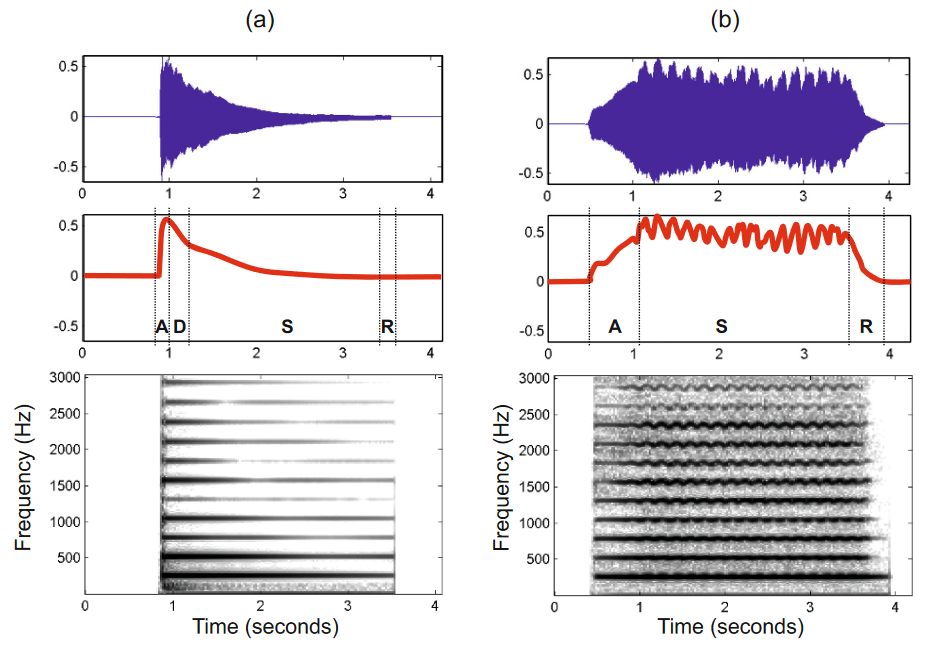
\includegraphics[width=0.9\textwidth]{resources/images/030-theoretical_framework/Framework_audio_fund_ADSR.png}
        \smallcaption{Source: \textcite{Mueller2016}, page 28}
        \label{fig:frmwk_audio_fund_adsr}
\end{figure}

The \textbf{threshold of audibility}, typically around 0 \gls{db} \gls{spl}, denotes the minimum sound level detectable by the human ear. In contrast, the threshold of pain, situated at approximately 120 \gls{db} \gls{spl}, represents the sound level at which sound becomes physically painful to the human ear. 

\textbf{\gls{adc}} involves two main processes: 
\begin{itemize}
    \item \textbf{Sampling} refers to capturing the value of an analog signal at discrete time intervals while \textbf{sampling rate} determines the number of samples taken per second and is measured in \gls{hz}. In CD audio, the sampling rate is 44,100 \gls{hz}, meaning 44,100 samples are taken per second;
    \item \textbf{Quantization} focuses on the amplitude of the signal, essentially dividing the range of possible amplitudes into discrete levels. The number of quantization levels determines the resolution of the digital signal.
\end{itemize}

A \textbf{digital signal} is represented by a sequence of discrete values, typically binary digits (bits). It differs from the analog electrical signals created by a microphone, which have a continuous range of values.

The \textbf{resolution of a digital signal} is often specified in terms of the number of bits used for quantization, also known as the bit depth. Common bit depths include 16, 24, and 32 bits, with 16 bits being the standard resolution for audio CDs. For 1 minute (60 seconds) of audio at a sampling rate of 44,100 \gls{hz} and a bit depth of 16 bits, the required memory is 5.17 \gls{m}\gls{b}, calculated using the formula: 

\begin{equation}
    \label{eq:frmwk_audio_fund_audio_memory_calculation}
\text{Memory (MB)} = \frac{\text{Sampling rate} \times \text{Bit depth} \times \text{Duration}}{8 \times 1024}
\end{equation}

The higher the bit depth (or resolution) of a digital audio signal, the greater the dynamic range it can capture and reproduce. A higher bit depth allows for a more accurate representation of subtle changes in amplitude.

The digitization process in the \gls{adc} involves the quantization of the signal in time at a specific sampling rate and the quantization of its amplitude at a particular bit-depth. With the typical audio CD values above, these parameters efficiently capture the majority of perceptible information in the acoustic sound. The resultant digital representation of sound takes the form of a one-dimensional sequence of numbers, also known as a waveform, as illustrated in the Figure \ref{fig:frmwk_audio_fund_digitization_process}.

\begin{figure}[htbp]
    \raggedright
        \caption{Two steps of a digitization process to transform an analog signal (solid curve) into a digital signal (stem plot). (a) Sampling. (b) Quantization.}
        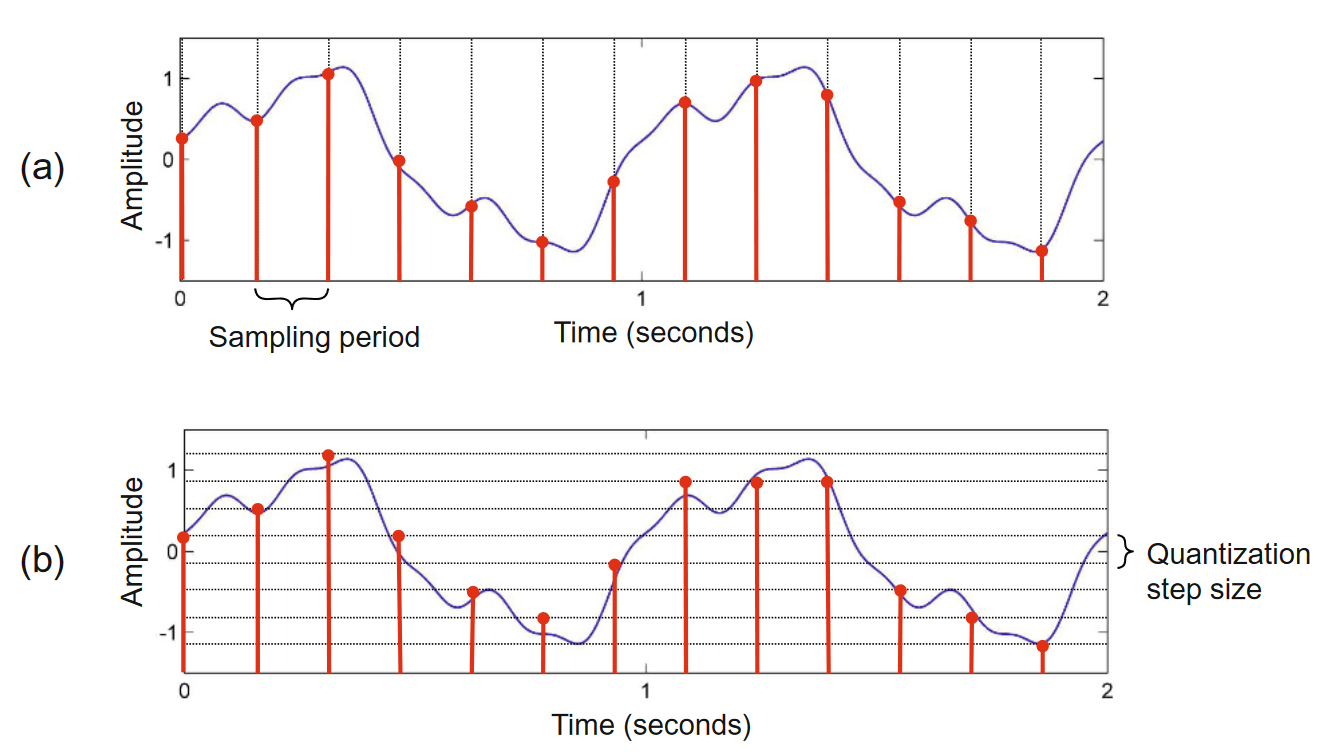
\includegraphics[width=1.0\textwidth]{resources/images/030-theoretical_framework/Framework_audio_fund_digitization_process.png}
        \smallcaption{Source: \textcite{Mueller2016}, page 61}
        \label{fig:frmwk_audio_fund_digitization_process}
\end{figure}

\textbf{Artifact} refers to an unintended and undesirable distortion or alteration of the audio signal that occurs during recording, transmission, processing, or playback. Artifacts can manifest as unwanted sounds, anomalies, or imperfections that degrade the quality of the audio signal.

According to the Nyquist-Shannon theorem, the \textbf{Nyquist frequency} is half of the sampling rate. It represents the highest frequency that can be accurately represented in a digital signal without introducing distortion.

A \textbf{spectrogram} is a visual representation of the frequency content of a signal over time. It displays how the intensity of different frequencies in the signal changes over time, typically with frequency on the vertical axis, time on the horizontal axis, and color or brightness representing intensity


\subsection{Digital audio analysis}
\label{subsec:audio_fundamentals_digital_audio_analsys}

The conventional method for analyzing signals in the spectral domain relies on classical Fourier analysis, which is applied to the entire signal shifting the information from the time domain to the frequency domain as shown in Figure \ref{fig:frmwk_digital_audio_fourier_transform}. However, the definition of the Fourier Transform faces challenges in audio signal analysis because real-world audio signals are time-varying. These signals are non-stationary and their significance is inherently linked to this temporal variability. Therefore, there is a crucial need to develop techniques for analyzing sound that can capture the important time-varying aspects of audio signals which are essential for tasks such as feature extraction and other audio analysis tasks.

\begin{figure}[htbp]
    \raggedright
        \caption{Example of Fourier Transform applied to an audio signal illustrating the switch from the time domain to the frequency domain.}
        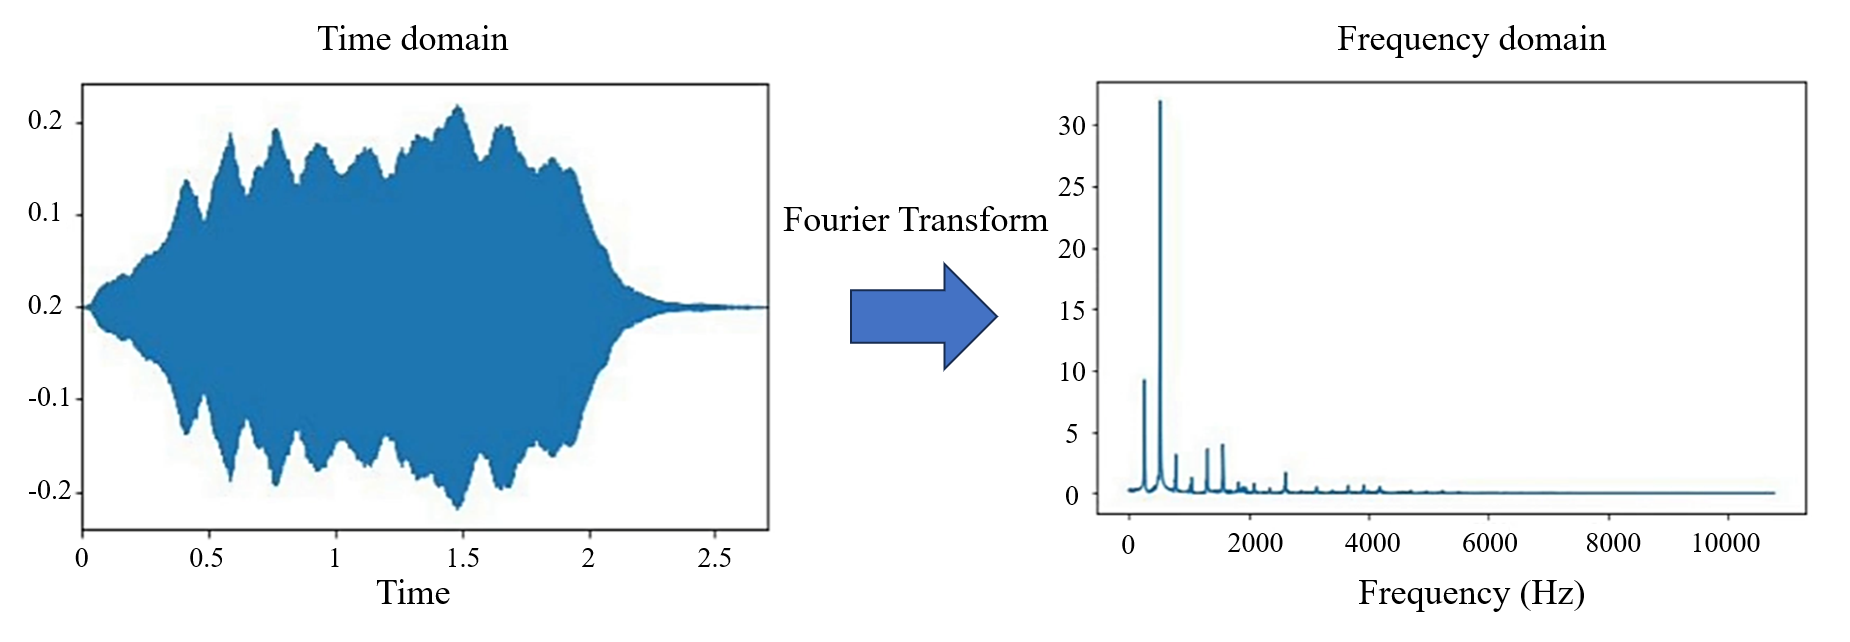
\includegraphics[width=1.0\textwidth]{resources/images/030-theoretical_framework/Framework_digital_audio_fourier_transform.png}
        \smallcaption{Source: Author}
        \label{fig:frmwk_digital_audio_fourier_transform}
\end{figure}

In order to overcome these challenges, the audio signal is initially divided into short segments called frames where each frame is specifically chosen to be brief enough to be considered approximately stationary. This segmentation process is commonly referred to as \textbf{Framing}. The duration of each frame typically ranges from 10 to 50 \gls{mi}\gls{s}, assuming that within such a short timeframe, the audio signal undergoes minimal changes. Audio processing tasks, such as Fourier Transform and feature extraction, are performed on a frame-by-frame basis. To ensure a smoother transition and minimize abrupt changes and discontinuities which causes spectral leakage in the signal, frames are often multiplied by smoothing functions, such as the Hanning window function, prior to applying Fourier Transform operations which renders this process the name \textbf{Windowing} \cite{Abreha2014}.

The technique of analyzing audio signals frame by frame is referred to as short-time signal analysis. In the existing literature \cite{Debnath2014}, there are various methods for short-time analysis, namely the \gls{stft}, Discrete Wavelet Transform (DWT), and Wigner-Ville Distribution (WVD). Among these, \gls{stft} stands out as the most commonly employed short-time analysis technique due to its computational simplicity.


\subsubsection{Short-Time Fourier Transform}
\label{subsubsec:audio_fundamentals_fourier_transform}

Joseph Fourier, born in 1768, made significant contributions to the field of mathematical physics, and he is particularly known for his work on heat transfer and the mathematical techniques he developed, including what is now known as the Fourier series and the Fourier Transform. His work on the decomposition of functions into sums of sinusoidal functions laid the foundation for the understanding of periodic functions and played a crucial role in various fields, including signal processing, communication theory, and quantum mechanics \cite{Debnath2014}.

The formula for the continuous complex Fourier Transform of a signal $f(t)$ is given by:

\begin{equation}
    \label{eq:frmwk_audio_fund_fft}
    \hat{f}(\omega)=\int_{-\infty}^{\infty} f(t) \cdot e^{-i \omega t} d t
\end{equation}

Where $\hat{f}(\omega)$ is the complex Fourier Transform of the signal at frequency $\omega$, the input signal is given by $f(t)$, the angular frequency by $\omega$, and the imaginary unit is $i$.

This formula involves integrating the product of the input signal and a complex exponential term over all time values $t$. The result is a complex-valued function of frequency $\omega$ that describes the frequency content of the input signal.

Given an analog signal $f : \mathbb{R} \rightarrow \mathbb{R}$ and a positive real number $T > 0$, the function $x : \mathbb{Z} \rightarrow \mathbb{R}$ is defined by $x(n):= f(n.T)$. Considering $x$ is defined only on a discrete set of time points, the value $x(n)$ is named \textbf{sample} taken at time $t = n.T$ of the original analog signal $f$ at the sampling period $T$, which is the inverse of the sampling rate.

In the context of discrete-time signals, the \gls{dft} is often used assuming, firstly, that most of the relevant information of $f$ is limited to a certain duration in time, resulting in a finite number of samples $x(0)$, $x(1)$, $\ldots$, $x(N-1)$ for some suitable number $N\in\mathbb{N} $, and secondly, one calculates the Fourier Transform for a limited set of frequencies. Analogous to discretizing the time axis, the frequency axis is commonly sampled with frequencies $\omega = k/M$ for some appropriate $M\in\mathbb{N} $ and $k \in [0: M-1]$. In practical applications, it is common to align the number $N$ of samples with the parameter $M$ determining the frequency resolution by setting $N = M$. It is essential to note that $N$ and $M$ refers to distinct aspects. Nevertheless, this alignment proves advantageous, ensuring not only the invertibility of the resulting transform but also yielding a computationally efficient algorithm \cite{Mueller2021}.

The formula for the \gls{dft} with integers $k \in[0:M-1]=[0:N-1]$ is given by:

\begin{equation}
    \label{eq:frmwk_audio_fund_dft}
    X(k) = \hat{x}(k / N)=\sum_{n=0}^{N-1} x(n) \cdot e^{-i 2 \pi n \frac{k}{N} }
\end{equation}

Where $\hat{x}(k/N)$ is the \gls{dft} of the signal at frequency index $k$, the input signal is $x(n)$, and $N$ is the length of the signal.

The \gls{dft} represents the frequency content of the signal at equally spaced frequency bins. In practice, the \gls{fft} algorithm is often used to efficiently compute the \gls{dft} by taking advantage of redundancies among sinusoids of various frequencies, allowing for the simultaneous computation of all Fourier coefficients through a recursive process. This recursion is especially effective when $N$ is a power of two, consequently, the \gls{fft} significantly decreases the total number of operations, reducing it from $O(N^2)$ to $O(N \log_2 N)$.

Instead of considering the entire domain of the signal which hides "when" the frequencies occur, Dennis Gabor introduced in 1946, the \glsdisp{stft}{Short-Time Fourier Transform} (\gls{stft}) by focusing on specific sections of the signal or \textbf{frames}. This is achieved by multiplying the original signal with a \textbf{window function}, which defines the section being considered. By shifting the window function across time and performing a Fourier Transform on each windowed signal, frequency information at different time instances can be obtained. In other words, the \gls{stft} breaks the signal into frames, which overlap with each other to reduce artifacts at the boundary and to create more instances for analysis. 

Let a discrete signal $x$ be a function that maps integers to real numbers $\mathbb{Z} \rightarrow \mathbb{R}$. This signal is obtained by sampling at a regular rate $F_s$, given in \gls{hz}. Now let $w : [0:N - 1] \rightarrow \mathbb{R}$ be a sampled window function of length $N \in \mathbb{N}$. For example, considering a rectangular window, $w(n) = 1$ for $n \in [0:N - 1]$, outside this window, at time parameters not within $[0:N - 1]$, $w(n)$ will be assumed to be 0. The length parameter $N$ determines the duration of the sections (frames) considered in terms of $N/F_s$ seconds. Additionally, the parameter $H$ is introduced, a positive integer referred to as the \textbf{hop length} which determines the number of samples by which the window is shifted across the signal \cite{Mueller2021}.

The formula for the discrete \gls{stft} $\mathcal{X}$ of the signal $x$ with $m \in \mathbb{Z}$ and $k \in [0:K]$ where $K = N/2$ (assuming that $N$ is even) is the frequency index associated with the Nyquist frequency is given by:

\begin{equation}
    \label{eq:frmwk_stft_discrete_stft}
    \mathcal{X}(m, k):=\sum_{n=0}^{N-1} x(n+m H) w(n) \cdot e^{-i 2 \pi n \frac{k}{N}}
\end{equation}

Where $\mathcal{X}(m, k)$ represents the $k^{th}$ Fourier coefficient for the $m^{th}$ time frame. For each time frame $m$, one gets a spectral vector of size $K+1$ given by its associated Fourier coefficients. The computational costs of each spectral vector amounts to a \gls{dft} of size $N$, and as previously mentioned, it's more efficiently calculated using \gls{fft}. Figure \ref{fig:frmwk_stft_windowing} depicts this windowing process using a rectangular window function and hop length of 50\%.

Assuming the total length (in samples) of an audio signal as $L$, the number of frames $m^{th}$ calculated using \gls{stft} is given by:

\begin{equation}
    \label{eq:frmwk_stft_frames}
    \text{Number of frames} = \left\lfloor \frac{L-N}{H} \right\rfloor + 1
\end{equation}

\begin{figure}[htbp]
    \raggedright
        \caption{Illustration of rectangular window function applied to an audio signal simulating the overlap of the frames.}
        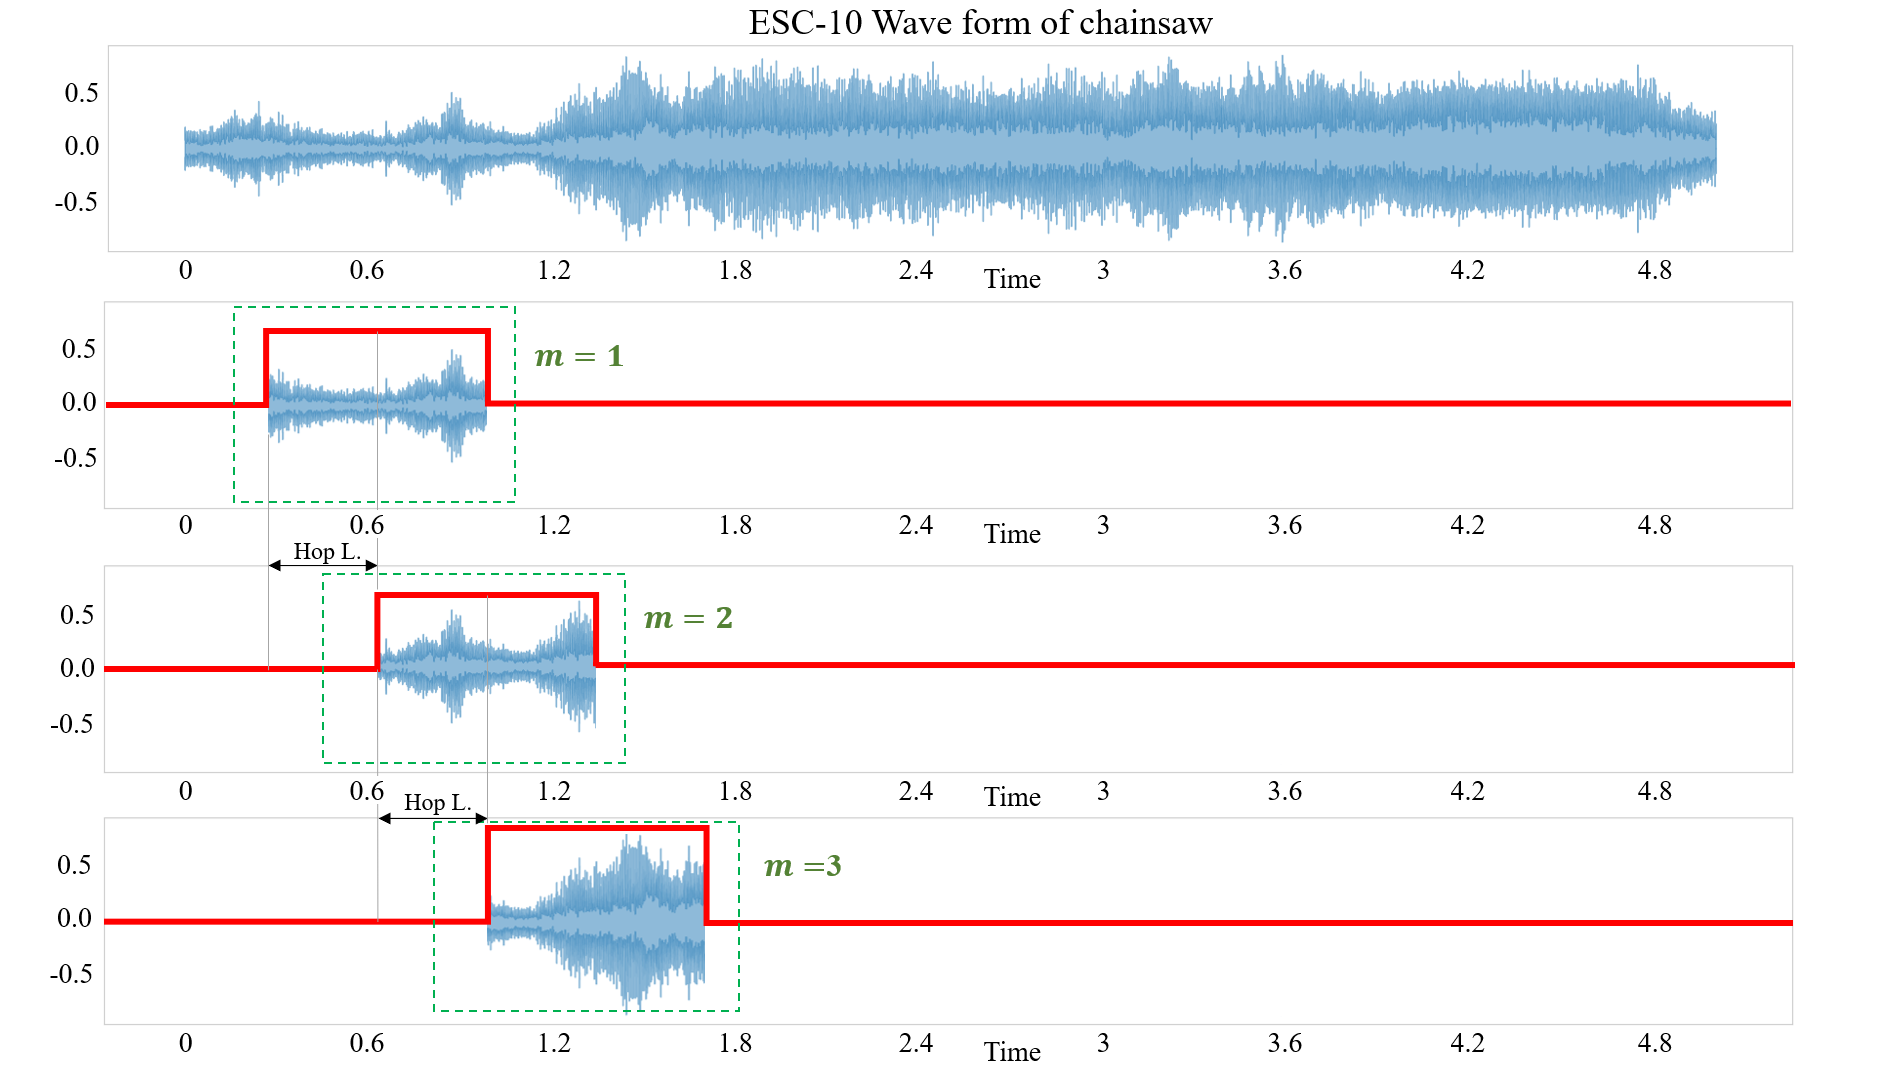
\includegraphics[width=1.0\textwidth]{resources/images/030-theoretical_framework/Framework_stft_windowing.png}
        \smallcaption{Source: Author}
        \label{fig:frmwk_stft_windowing}
\end{figure}


\subsubsection{Windows for the Short Time Fourier Transform}
\label{subsubsec:audio_fundamentals_windowing_techniques}

As already described, in audio analysis, techniques such as \gls{stft} are used to analyze sound by dividing the audio signal into smaller time segments called frames.  The length of each frame is typically chosen to balance the trade-off between time and frequency resolution and overlapping frames are often used to improve the time resolution of the analysis. In the literature, a few types of framing have been utilized according the end application, for example, \textcite{Preece2009} describe three types of framing to identify activities using body-mounted sensors: sliding windows, event-defined windows and activity-defined windows.

 Various window sizes have been utilized in earlier research, with some studies incorporating variable overlap between neighboring windows. Notably, the sliding window technique is straightforward and advantageous for real-time applications as it eliminates the need for pre-processing the audio signal. Its simplicity of implementation has made it the most commonly used approach for audio analysis and classification studies.

Considering the sliding window technique as the mainstream, the frames have to be synchronized or filtered using window functions. Several different windows are available named after their original developers in the 1950s, namely: Hamming window, Blackman window, Bartlett window (triangular), Hanning window (raised cosine window) and rectangular window \cite{Smith2013}, the last three illustrated in Figure \ref{fig:frmwk_windows_stft_example}. In \gls{stft}, a window function plays a crucial role in mitigating spectral leakage and also managing trade-offs between time and frequency resolution by tapering the signal smoothly to zero at the edges thus minimizing abrupt transitions. The choice of window function influences the balance between main lobe width and side lobe levels, impacting the resolution of both time and frequency components in the resulting spectrogram. Named after Julius Von Hann, the \textbf{Hanning window} is one of the most used window in signal processing according to \textcite{Mueller2021}.

\begin{figure}[htbp]
    \raggedright
        \caption{Windowed chirp signal and its magnitude Fourier Transform using different window functions. (a) Rectangular window. (b) Triangular window. (c) Hanning window.}
        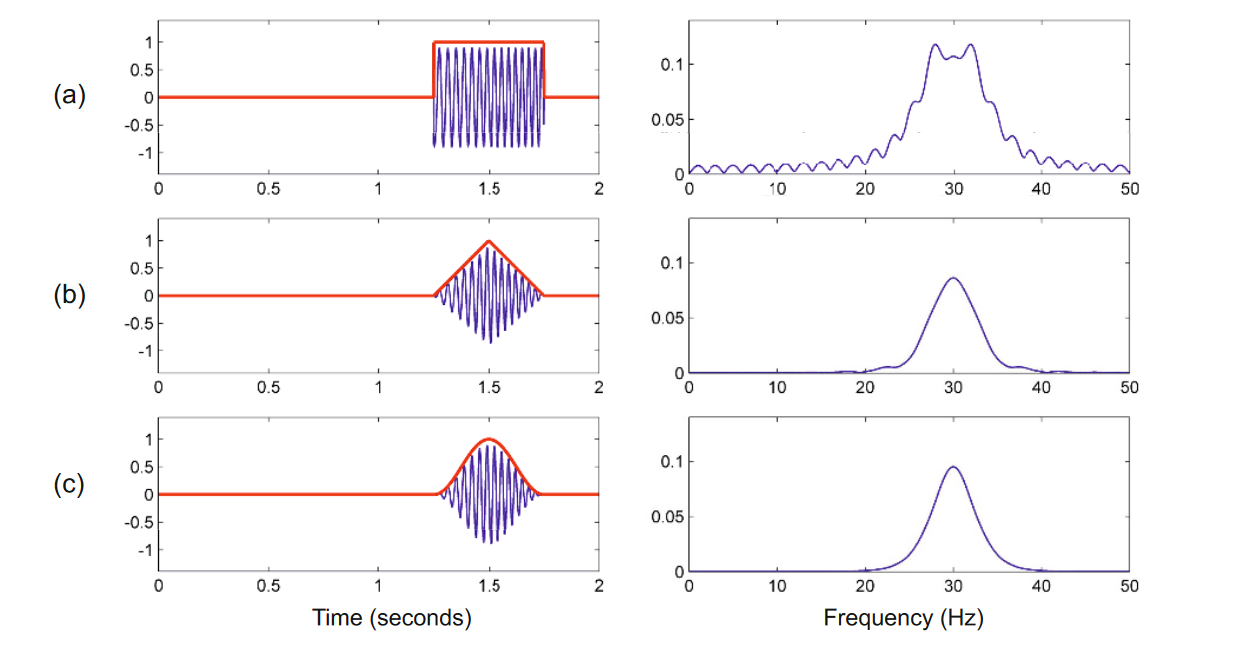
\includegraphics[width=1.0\textwidth]{resources/images/030-theoretical_framework/Framework_windows_stft_examples.png}
        \smallcaption{Source: \textcite{Mueller2021}, page 98}
        \label{fig:frmwk_windows_stft_example}
\end{figure}

Usually, the frame size and the Hanning window size have equal number of samples, although in some situations, one may choose different values for each one of them. Considering $w(n)$ is the value of the window at sample index $n$, and $N$ is the total number of samples in the window with $0 \leq n \leq N-1$, the Hanning window is mathematically defined according to \textcite{Smith2013} as:

\begin{equation}
    \label{eq:frmwk_windows_stft}
    w(n) = 0.5 - 0.5 \cos\left(\frac{2 \pi n}{N-1}\right)
\end{equation}


\subsubsection{Window function parameters}
\label{subsubsec:audio_fundamentals_window_function_parameters}

When performing a \gls{stft} using methods from specialized Python libraries such as openSMILE 3.0 \cite{Eyben2010} or \index{Librosa} Librosa \cite{McFee2015librosa_conf}, there are essentially three parameters that influence the result: window type, window size and overlapping size or hop length.

The choice of \textbf{window type} affects directly the resulting of the signal spectrogram. For instance, rectangular windows have a wide main lobe, providing high spectral resolution but suffer from significant spectral leakage due to high side lobes which causes a suddenly interruption of the signal at its edges, possibly leading to incorrect estimations of frequency components. On the other hand, window types like Hamming and Hanning have narrow main lobes and lower side lobes which reduces the signal's values towards zero at the edges of the window, preventing abrupt changes, resulting in a smoother spectrogram with reduced spectral leakage. The selection of an appropriate window type depends on the specific requirements of the application, such as the desired frequency resolution and the ability to distinguish between closely spaced spectral components \cite{Zoelzer2008}.

The \textbf{window size} parameter plays a vital role in determining the trade-off between time and frequency resolutions in the \gls{stft} analysis. Assumption within one frame, the signal is stationary, the window size directly influences the temporal and frequency granularity of the resulting spectrogram. A smaller window size provides better temporal resolution, enabling the identification of rapid changes in the audio signal, however, it comes at the cost of reduced frequency resolution, making it challenging to accurately distinguish between closely spaced frequency components. Conversely, a larger window size improves frequency resolution but compromises temporal resolution. The choice of window size is typically application-dependent, where tasks requiring fine spectral details may necessitate smaller window sizes, while tasks focusing on temporal dynamics may benefit from larger window sizes. Notably, the terms "window size" and "frame size" refer to slightly different aspects but are closely related: the window size specifically refers to the length or duration (in samples) of the window function that is applied to segments of the audio signal during the \gls{stft} analysis while the frame size refers to the duration of the segments (in samples) into which the audio signal is divided before applying the window function \cite{Smith2013}. The output vector from a $N$-sample \gls{dft} of the audio signal sampled at $F_s$ results in $N/2 +1$ frequency bins, with each bin capturing the energy from a small range of frequencies in the original signal \cite{Abreha2014}, hence, the output vector of the \gls{stft} applied to $N$ samples results in array of dimension: [frequency bins , number of frames] where the number of frames is given by equation \ref{eq:frmwk_stft_frames}. Most Python libraries implement their methods considering the window size and frame size to be identical, with the only option being to specify the frame size.

The process of overlapping frames guarantees that audio features present at a discontinuity are included in their entirety in the subsequent overlapped frame. The \textbf{overlapping size}, typically measured as a percentage, indicates the extent to which the previous frame is replicated in the following frame. Similar to selecting the window size, choosing the appropriate overlap size heavily depends on the specific objectives of the analysis or application. Generally, increasing the amount of overlap results in more analysis points and thus yields smoother results over time, potentially enhancing recognition accuracy in classification algorithms, however, this also leads to a proportional increase in computational cost. In Librosa \cite{McFee2015librosa_sw}, this parameter is named \textbf{hop length} and inputs an integer representing the number of samples overlapped.


\subsection{Audio features}
\label{subsec:audio_fundamentals_audio_features}

Essentially, there are two main types of audio features commonly used in the field of audio analysis: \textbf{physical features} and \textbf{perceptual features}. Physical features involve mathematical measurements derived directly from the sound wave, including the energy function, spectrum, cepstral coefficients, and fundamental frequency. On the other hand, perceptual features are subjective terms that relate to how sounds are perceived by humans, encompassing aspects such as loudness, brightness, pitch, timbre, and rhythm \cite{Zhang2010} and \cite{Alias2016}. Further on, physical features are further classified into \textbf{temporal features} and \textbf{spectral features}\footnote{For simplicity, frequency, image and cepstral domains were all compiled in this classification}, which are based on the signal domain categorization. The selection of the following specific physical features for use in \gls{esr} applications was based on a comprehensive literature review presented in the related work chapter, but before that, a few definitions regarding feature categorization and requirements for feature selection are given.


\subsubsection{Requirements for selecting the audio features}
\label{subsubsec:audio_features_requirements_for_selecting_features}

Within the existing literature, numerous methods for extracting audio features are documented. The effectiveness of \gls{esr} heavily relies on the choice of audio feature extraction techniques utilized, and consequently, the careful selection of audio features becomes crucial in achieving optimal performance and accurate recognition. Even when constraining the application to \gls{esr}, the the choice of audio features depends on the application’s type and purpose, particularly in resource-constrained devices like those used in the automotive industry, specifically for autonomous vehicles. The requirements for such implementation include multi-kernel support for end-to-end hybrid algorithms, real-time low-latency operation to quickly respond to each target event, and an optimized energy efficiency to reduce the overall vehicle power budget \cite{Yin2023}, nevertheless, these requirements can affect the recognition accuracy. Therefore, the selection of audio features should aim to develop a technique with low computational complexity, fast response time in the context of automotive applications, low energy consumption, and memory requirement, while still providing acceptable recognition accuracy. Given these requirements, the selection of audio features should include a small feature size to minimize computational cost, low computational complexity, high inter-class variability for improved discrimination between audio patterns, high intra-class similarity to decrease discrimination among similar classes, and low sensitivity to minor changes in the signal for robustness against noise and other sources of interference.


\subsubsection{Temporal features}
\label{subsubsec:audio_features_temporal}

Temporal features refer to characteristics or attributes of sound signals that evolve over time, making the temporal domain the native representation domain for audio signals. Extracted directly from the raw audio signal, temporal features do not require any preceding transformation, keeping the computational complexity low in comparison to spectral features. These features provide valuable information about the temporal dynamics of the audio signal. The temporal features included in this study are: \textbf{\gls{zcr}} and \textbf{\gls{rms}}.

\textbf{\gls{zcr}} is a low level feature that captures the rate of transitions between positive and negative values within a signal, in other words,  the smoothness of a signal by counting the number of times the signal crosses the zero axis within a segment of that signal. It finds widespread application in fields such as speech recognition, music information retrieval, and percussive sound classification. Additionally, \gls{zcr} proves valuable in tasks like basic pitch detection for monophonic tonal signals and voice activity detection to ascertain the presence of human speech within audio segments \cite{Park2008}, it's sensitive to noise though. 

\textbf{\gls{rms}} is another low level feature that calculates the average energy of a frame and is an indicator of loudness which corresponds more closely to our hearing system’s sensitivity to the change in intensity of audio signals. It is less sensitive to outliers compared to amplitude envelops and finds applications in audio segmentation and music genre classification. 


\subsubsection{Spectral features}
\label{subsubsec:spectral_fatures}

Spectral features refer to the characteristics or attributes extracted from the frequency domain representation of an audio signal aiming to capture specific spectral patterns or properties present in the signal. \textcite{Peeters2004} presents a large set of audio features and most of them dwell in the frequency domain, so it's imperative to select the spectral features carefully. Each frequency or frequency bin provides information about its magnitude and phase, given that changes in phase have little impact on the perceived sound, there is no need to focus on features that analyze phase. Instead, the focus shifted to features that capture basic properties of the sound's frequency distribution. Additionally the spectral features utilized by \textcite{Lhoest2021}, \textcite{Silva2019}, and \textcite{Bountourakis2015}, provided a reliable direction. The spectral features included in this study are: \textbf{\gls{sc}}, \textbf{\gls{sb}}, \textbf{\gls{srp}}, \textbf{\gls{sct}}, \textbf{Tonnetz}, \textbf{Chroma feature}, \textbf{Mel spectrogram}, \textbf{\glsdisp{mfcc}{Mel-Frequency Cepstral Coefficients} (\gls{mfcc})}, and two feature manipulations namely: \textbf{Delta \gls{mfcc}} and \textbf{Delta-Delta \gls{mfcc}}.

\textbf{\glsdisp{sc}{Spectral Centroid} (\gls{sc})} can be interpreted as the "center of mass" or "center of gravity" of the spectrum of a audio signal. It is a measure of where the "center" of the spectral content of an audio signal lies in terms of frequency and it is often used to describe the perceived "brightness" or "timbre" of a sound, and for that reason, sometimes is also addressed as a perceptual feature. It is a useful feature for distinguishing between different types of sounds based on their spectral characteristics. %(Figure \ref{fig:frmwk_spectral_features_sc})
For example, sounds with higher spectral centroids tend to have a brighter or more treble-heavy quality, while those with lower centroids are generally more bass-heavy or darker in timbre \cite{Park2008}.

\textbf{\glsdisp{sb}{Spectral Bandwidth} (\gls{sb})} is another important feature that characterizes the width or spread of the frequency content in an audio signal's spectrum. It provides information about how concentrated or dispersed the spectral energy is across different frequency components. It has also a perceptual definition which is commonly associated with the perceived "sharpness" or "clarity" of a sound. A higher spectral bandwidth indicates that the spectral energy is spread out over a wider range of frequencies, which can result in a sound that is perceived as being more complex or noisy. In contrast, a lower spectral bandwidth suggests that the energy is concentrated around a narrow band of frequencies, leading to a cleaner or purer sound \cite{Park2008}.

The \index{Librosa}Librosa \cite{McFee2015librosa_sw} method to extract \gls{sb} is based on \textcite{Klapuri2006}, but instead of calculating the second central moment of the spectrum, also known as spectral spread, using $p=2$, it enables the computation of the $p-th$ root of the sum, where $p$ is left an input parameter ($p$ determines the "order" of the bandwidth calculation). 

\textbf{\glsdisp{srp}{Spectral Rolloff Point} (\gls{srp})} characterizes the frequency below which a specified percentage (often a threshold like 85\% or 95\%) of the total spectral energy lies and it provides information about the lower boundary of the frequency range where most of the energy in an audio signal is concentrated. A higher spectral rolloff value indicates that the majority of the spectral energy is contained in lower frequencies, while a lower value suggests that energy extends into higher frequencies.

This feature is valuable for discerning voiced speech from unvoiced speech: the latter, including most of the environmental sounds, typically exhibits a significant concentration of energy in the higher frequency range of the spectrum, whereas voiced speech and music tend to have the majority of their energy concentrated in lower frequency bands. \cite{Giannakopoulos2014}. This study adopted the threshold of 85\%.

\textbf{\glsdisp{sct}{Spectral Contrast} (\gls{sct})} represents a way to describe the tonal characteristics or timbre of an audio signal. It is a feature that quantifies the difference in spectral energy between peaks and valleys in the frequency spectrum of an audio signal. Higher spectral contrast indicates greater variation in energy levels across frequency bands, which can lead to a perception of greater clarity and distinction between different parts of the sound spectrum. This can be relevant in tasks such as speech recognition, music analysis, and sound classification, where distinguishing between different frequency components is important for understanding the content of the audio signal \cite{Jiang2002}.

Given a frequency domain divided into six Octave-scale sub-bands (0-200, 200-400, 400-800, 800-1,600, 1,600-3,200, and 3,200-8,000 \gls{hz}), \gls{sct} is computed by calculating the difference in energy between the maximum and minimum spectral values within each sub-band. The result is a multi-dimensional vector representing the contrast in energy between different frequency regions represented by the sub-bands.

\textbf{Chroma Feature} represents a way to describe the harmonic content or pitch class of an audio signal. It is a feature that characterizes the distribution of musical pitches (notes) in an audio signal, ignoring the octave or absolute frequency information. Chroma Features are typically computed using a chromagram, which is a representation of the 12 different pitch classes in Western music corresponding to the 12 semitones in an octave (e.g., C, C\#, D, D\#, E, F, F\#, G, G\#, A, A\#, B). One way to calculate Chroma Feature is, first the audio signal is transformed into the frequency domain using techniques such the \gls{dft}, then, for each short time frame of audio, the energy or magnitude of each of the 12 pitch classes is measured, resulting in a 12-dimensional vector that represents the presence or strength of each pitch class in that time frame \cite{Bartsch2005}.

Although similar in concept, Chroma Feature and \gls{sct} capture different aspects of the audio signal. Chroma Feature summarize the distribution of energy in different pitch classes over time, \gls{sct}, on the other hand, focuses on capturing the difference in energy between peaks and valleys in the frequency spectrum. Chroma Features are computed by grouping frequency bins in the \gls{dft} spectrogram that correspond to the same pitch class and summing their magnitudes while \gls{sct} is computed by dividing the spectrum into sub-bands, computing the mean energy within each sub-band, and then calculating the difference between the maximum and minimum energy across adjacent sub-bands.

\textbf{Tonnetz} represents a way to describe the tonal relationships or harmonic structure of an audio signal that characterizes the tonal distance between musical pitches (notes) in an audio signal using the concept of tonnetz, which is a two-dimensional representation of pitch space. To calculate Tonnetz features, first the Chroma Features are extracted using the \gls{stft}, then the Chroma Features are converted to Tonnetz representation by using Euler's Tonnetz transformation. The result is a two-dimensional matrix or feature vector representing the tonal relationships between different pitch classes \cite{Harte2006}.

\index{Librosa}Librosa returns a vector  [6, $N$] where each row of Tonnetz values corresponds to the tonal centroid features for each frame $N$. The vector dimensions represents 0: Fifth x-axis, 1: Fifth y-axis, 2: Minor x-axis, 3: Minor y-axis, 4: Major x-axis and 5: Major y-axis.


The \textbf{Mel} Scale represents a significant advancement in our understanding of how humans perceive frequencies. Research has revealed that our perception of frequencies is not linear; rather, we exhibit greater sensitivity to differences in lower frequencies compared to higher ones. To illustrate, distinguishing between 500 and 1,000 \gls{hz} is relatively straightforward, while discerning a difference between 10,000 and 10,500 \gls{hz} proves considerably more challenging, despite the equal numerical interval between the two pairs. 

In 1937, the concept of the Mel scale was introduced by Stevens, Volkmann, and Newmann as a unit of pitch, designed to ensure that equal pitch intervals sounded equally spaced to the human ear. The name "Mel" originates from the musical term "melody," highlighting its connection to the frequency aspect of musical compositions and the measurement of pitch-related perceptual distances within melodies. To achieve this, a mathematical transformation is applied to frequencies, converting them into the \textbf{Mel scale}, thereby aligning auditory perception more closely with human sensitivity to frequency differences, in other words, the Mel scale is constructed such that sounds of equal distance from each other on the Mel scale, also “sound” to humans as they are equal in distance from one another having less resolution at high frequencies and a finer resolution at low frequencies \cite{Moore2013}. 

\textcite{Park2008} presents the original Mel scale curve in Figure \ref{fig:frmwk_spectral_features_mel_scale} (a) when $f_c$ is equal to $m$ at $f_c = 1$ \gls{k}\gls{hz} — the reference point between Mel frequency and frequency in Hertz, where 1 \gls{k}\gls{hz} is equal to 1,000 mels (the reference \gls{db} is 40 \gls{db} above the threshold of hearing). 

\begin{figure}[htbp]
    \raggedright
        \caption{Original Mel scale curve illustrating the intersection point where $f_c$ = 1\gls{k}\gls{hz} = 1,000 mels (a), and the common implementation utilized in Python and Matlab libraries with a linear response below $f_c$ = 1 \gls{k}\gls{hz} (b).}
        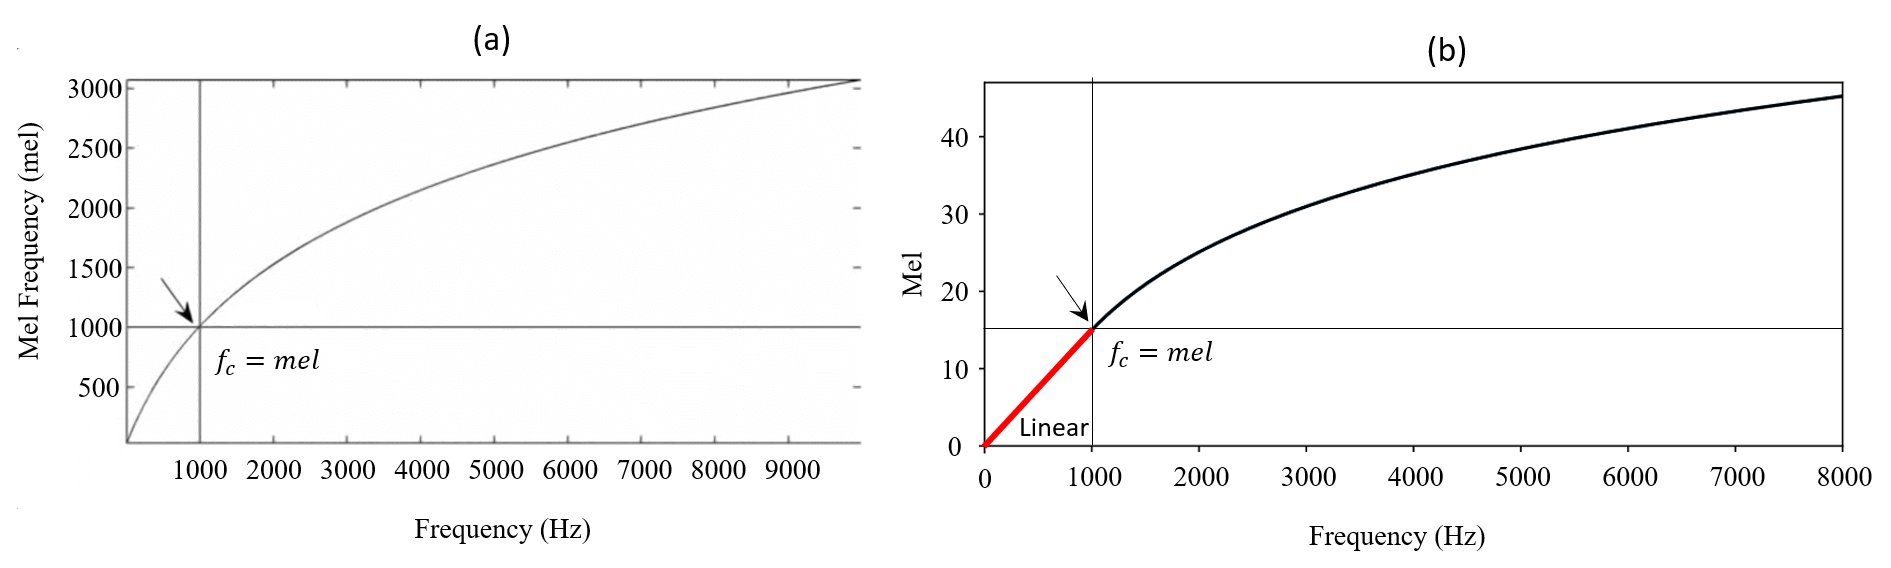
\includegraphics[width=1\textwidth]{resources/images/030-theoretical_framework/Framework_spectral_features_log-mel_scale.png}
        \smallcaption{Source: Author (a) "adapted from" \textcite{Park2008}, page 418, (b) "adapted from" \textcite{Rothmund2018}, page 68}
        \label{fig:frmwk_spectral_features_mel_scale}
\end{figure}

However, most current implementation in Matlab and Python, including \index{Librosa}Libosa, consider the auditory system’s frequency response as linear below $f_c = 1$ \gls{k}\gls{hz}, and upwards of $f_c$, the frequency resolution decreases incrementally as depicted in Figure \ref{fig:frmwk_spectral_features_mel_scale} (b). 

\textbf{Mel spectrograms} are calculated by first computing \gls{stft} of the audio signal and then mapping the result to the corresponding Mel scale using a mapping matrix. The matrix is based on $M$ triangular filters where each filter is scaled so that the area under each triangle is constant as illustrated by Figure \ref{fig:frmwk_spectral_features_mel_filter_bank}. \index{Librosa}Librosa \cite{McFee2015librosa_sw} returns a vector [$M, N$] where each row of Mel band $m$ has the Mel-spectrogram magnitude of the frequency bins $k$.

\begin{figure}[htbp]
    \raggedright
        \caption{Mel-weighting filter bank consisting of 8 triangular filters combing linearly spaced frequency bins between 0 and 8 \gls{k}\gls{hz} into 8 Mel bands from 100 \gls{hz} to 6 \gls{k}\gls{hz}}
        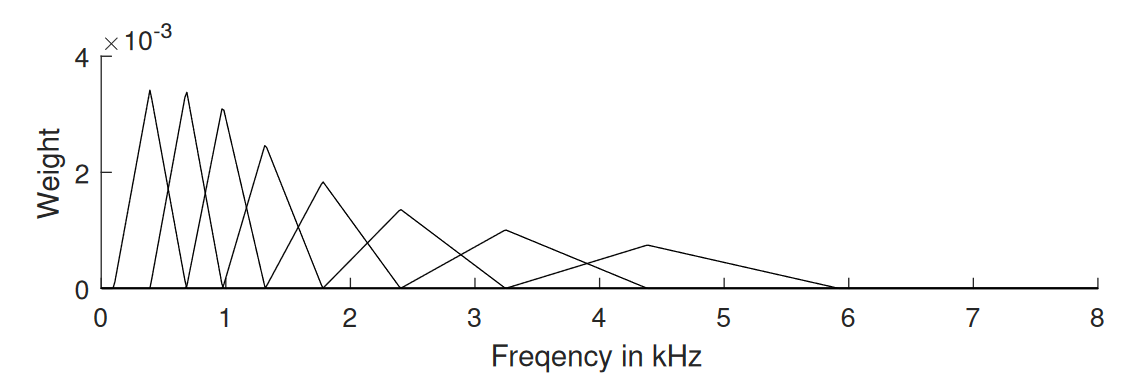
\includegraphics[width=.75\textwidth]{resources/images/030-theoretical_framework/Framework_spectral_features_log-mel_filter_bank.png}
        \smallcaption{Source: \textcite{Rothmund2018}, page 69}
        \label{fig:frmwk_spectral_features_mel_filter_bank}
\end{figure}

The concept of \textbf{\glsdisp{mfcc}{Mel-Frequency Cepstral Coefficients} (\gls{mfcc})} was originally introduced in the 1980s for speech recognition tasks \cite{DavisMermelstein1980}, aimed to address the limitations of simple spectral analysis techniques, which were found to be inadequate for representing the characteristics of human speech. Cepstrum and quefrency were coined by swapping the initial syllables of spectrum and frequency. According to \textcite{Oppenheim2004}, this consonant exchange illustrates the cross-disciplinary approach, where techniques typically used in the time domain are applied to frequency analysis, and vice versa. Although very popular in the field of speech recognition, it also found space in the field of audio classification being rated as the most utilized feature extraction technique in the systematic review of data augmentation and deep learning methods in sound classification \cite{Alli2022}.

The computation of \gls{mfcc} involves several steps according to \textcite{Klapuri2006}:

\begin{itemize}
    \item A pre-emphasis filter is applied to flatten the spectrum;
    \item The audio signal is framed, windowed and transformed using the \gls{dft};
    \item A Mel-scale filter bank is applied in the frequency domain, as previously explained;
    \item The power within each sub-band is computed by squaring and summing frequency bin magnitudes within bands;
    \item The dynamic range of the spectrum is compressed by taking a logarithm of the band wise power values;
    \item Finally, cepstral coefficients are computed by applying, to the log filter bank powers, the \gls{dct}\footnote{The Discrete Cosine Transform is similar to the \gls{dft} but only uses the cosine function to represent the signal.} which decorrelates the coefficients as:
\end{itemize}

The dimensionality of the representation can be reduced by retaining only approximately 13 lowest-order \gls{dct}, which usually carry the relevant timbral information. Succinctly the first \gls{dct} coefficient serves to denote the average power or energy in the spectrum, the second coefficient offers an approximation of the spectrum's broad shape and maintains a relation to the spectral centroid whereas for the higher-order coefficients, they capture finer spectral details such as pitch. Typically, in practice, a subset ranging from the first 8 to 13 \gls{mfcc} coefficients adequately represents the spectrum's shape, with the higher-order coefficients being disregarded due to their redundancy in providing additional information \cite{Abreha2014}. Librosa returns a vector [$\sum i, N$] where each row $i$ has the \gls{mfcc} coefficients of the frequency bins $k$.

\gls{mfcc} has one significant limitation which is its sensitivity to noise and channel variations. If the audio signal is corrupted with noise or transmitted through a poor-quality channel, the extracted \gls{mfcc} coefficients may not accurately represent the underlying sound information. Another limitation is the lack of temporal information in the \gls{mfcc} representation. Since the computation of \gls{mfcc} is frame-based, it does not capture the dynamics and temporal variations of the speech signal. To alleviate this limitation, dynamic features such as delta and acceleration coefficients are commonly computed by taking the derivatives of \gls{mfcc} \cite{Gold2011}. To illustrate this concept, Figure \ref{fig:frmwk_spectral_features_mfcc} compares the spectrograms of the \gls{mfcc} (first row), $\triangle$\gls{mfcc} (second row) and $\triangle\triangle$\gls{mfcc} (third row) set to 13 coefficients for five samples from the ESC-10 dataset, 

\begin{figure}[htbp]
    \raggedright
        \caption{Example of \gls{mfcc}, $\triangle$\gls{mfcc}, and $\triangle\triangle$\gls{mfcc} plot applied to random samples of the dataset ESC-10.}
        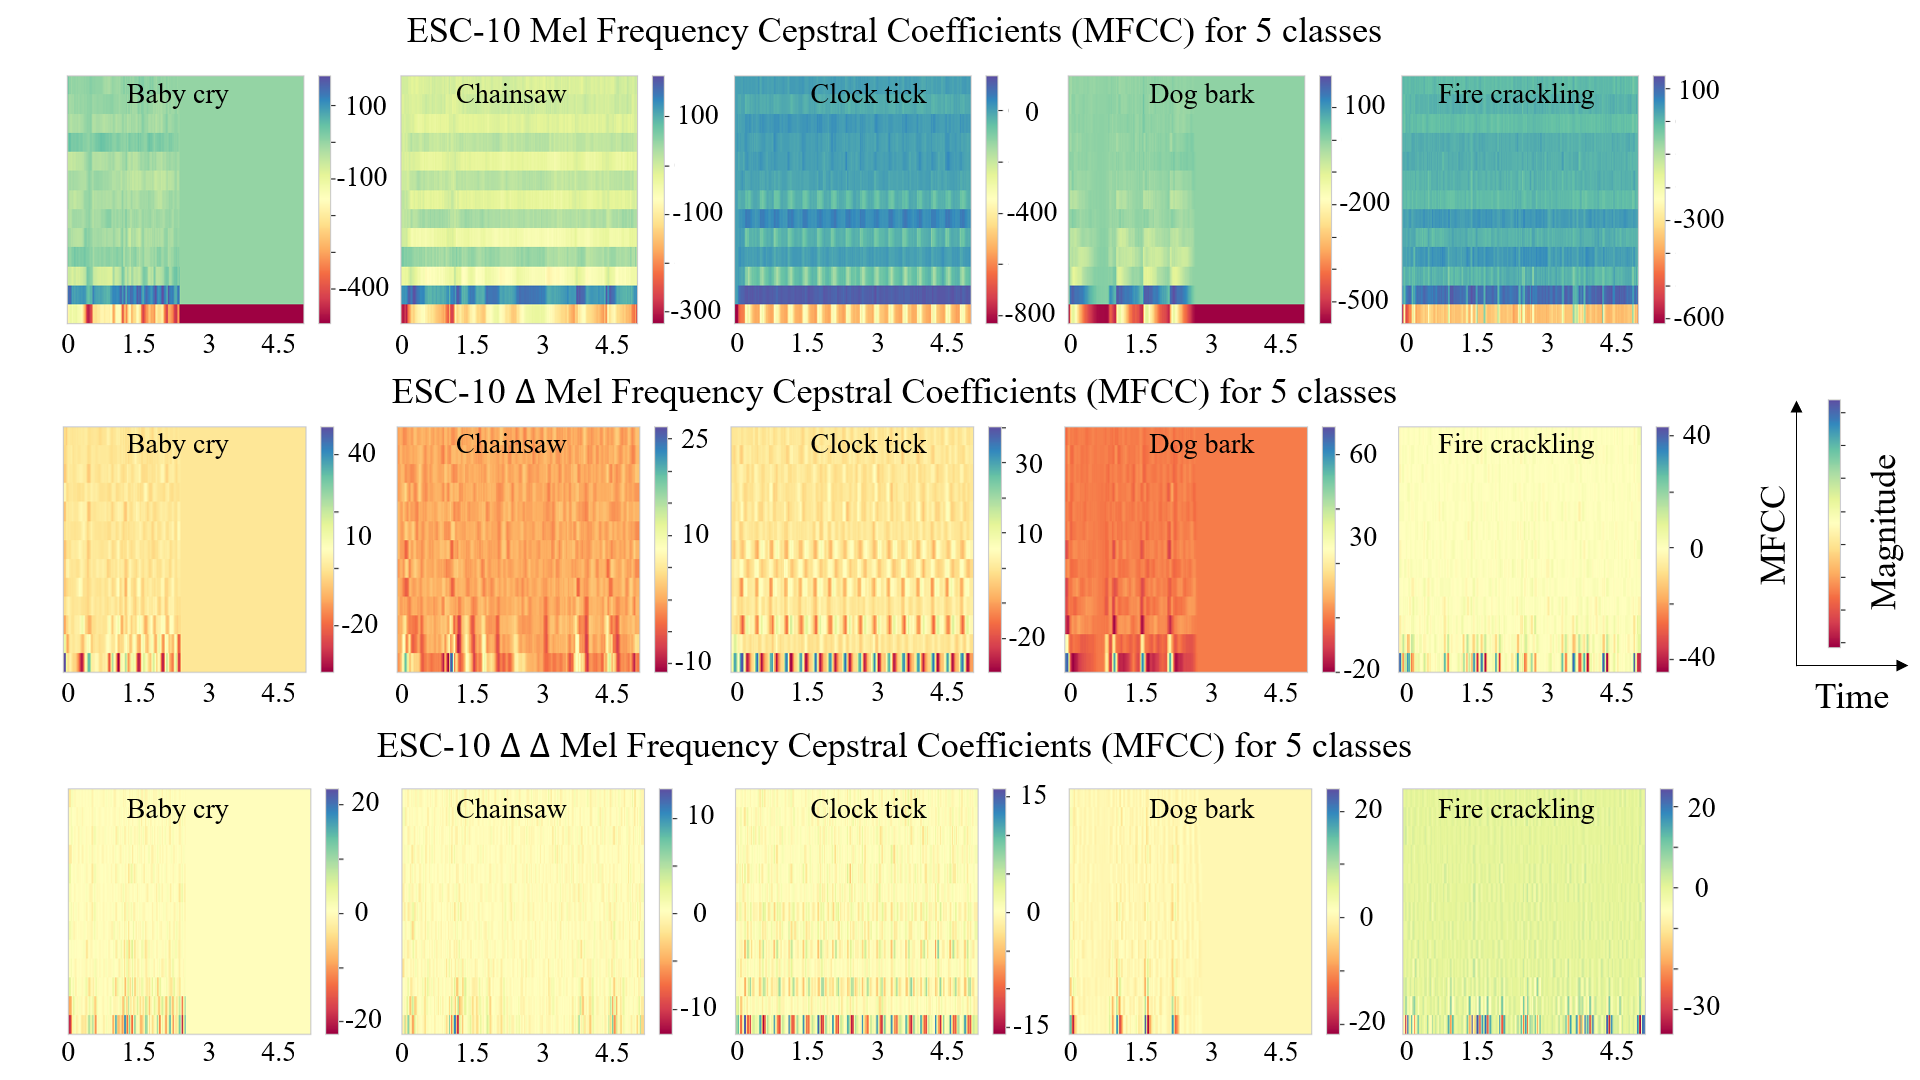
\includegraphics[width=1.0\textwidth]{resources/images/030-theoretical_framework/Framework_spectral_features_mfcc.png}
        \smallcaption{Source: Author}
        \label{fig:frmwk_spectral_features_mfcc}
\end{figure}

\textbf{Delta \gls{mfcc}} and \textbf{Delta-Delta \gls{mfcc}}, also know as \textbf{$\triangle$\gls{mfcc}} and \textbf{$\triangle\triangle$\gls{mfcc}} are the first and second order derivative of the \gls{mfcc} along the time axis. The first captures information about the velocity or speed of changes in the audio features and the latter captures the rate of change of the $\triangle$\gls{mfcc} coefficients, capturing the curvature or acceleration of the spectral features. Both $\triangle$\gls{mfcc} and $\triangle\triangle$\gls{mfcc} are often concatenated with the original \gls{mfcc} coefficients to form a feature vector that incorporates temporal dynamics \cite{Bountourakis2019} and \cite{Tang2018}. 


\subsection{Conclusion}
\label{subsec:audio_fundamentals_conclusion}

Based on the detailed exploration of audio feature extraction techniques in the context of \gls{esr}, it became evident that the selection of appropriate audio features plays a critical role in achieving optimal performance and accurate recognition. The unique requirements of \gls{esr} for autonomous vehicles, such as multi-kernel support, real-time operation, energy efficiency, and memory optimization, present challenges that must be carefully considered when choosing audio features. The ideal audio features for such applications should exhibit low computational complexity, fast response time, minimal energy consumption, and memory usage while maintaining acceptable recognition accuracy, all that can be achieved with the selected features using \gls{stft}. Additionally, the selected audio features should possess a small feature size to reduce computational costs, and therefore, \gls{mfcc}, \gls{sct}, Chroma and Tonnetz must be carefully assessed regarding their influence in the classification metrics.


\section{MICROPHONES}
\label{sec:frmwk_microphones}

This section introduces relevant definitions, concepts and characteristics related to microphones, hearing capabilities and their applications in the automotive industry.


\subsection{Definitions}
\label{subsec:microphones_definitions}

In psychoacoustics, \textbf{sensitivity} is the ability of the human ear to detect and comprehend sounds at various frequencies and intensities, measuring how well an individual can perceive and differentiate sounds at various levels of volume or loudness \cite{Moore2013}.

In a microphone, \textbf{sensitivity} represents the ability to convert sound waves into an electrical signal. It measures how well a microphone can collect and detect sound, especially low-level or quiet noises, which means, a microphone's sensitivity dictates how responsive it is to sound pressure levels and influences its ability to capture quiet or distant sounds accurately. Sensitivity is often evaluated as the \gls{spl} necessary to achieve a specific output level from the microphone and is usually represented in \gls{db}. The higher the sensitivity rating in \gls{db}, the more sensitive the microphone to sound \cite{Rayburn2004}.

\textbf{\gls{fr}} refers to how well the human ear can perceive sound at different frequencies in psychoacoustics. It is a measure of the sensitivity of the human ear to sound at different frequencies, and it plays an important role in determining how humans perceive and interpret different sounds. The human ear's frequency sensitivity does not remain constant across all frequencies, rather some frequencies are more responsive to the ear than others. A \gls{fr} curve, which illustrates how well the ear responds to different frequencies, can be used to measure this sensitivity, and it typically depicts the amount of sound pressure required for a listener to perceive a sound at a specific frequency, measured in \gls{db} and plotted with frequency (in \gls{db}) on the horizontal axis and \gls{spl} on the vertical axis \cite{Moore2013}.

In a comparable manner, \textbf{\gls{fr}} in a microphone refers to how it responds to different frequencies across the audible spectrum, in other words, it describes the microphone's ability to capture and reproduce sound accurately at various frequencies \cite{Rayburn2004}.

A microphone's frequency response is often displayed as a graph or numerical specification that demonstrates how the sensitivity of the microphone fluctuates across the frequency range. According to \textcite{Rayburn2004}, it illustrates which frequencies are more responsive to the microphone and how it attenuates or highlights specific frequency ranges as shown in Figure \ref{fig:frmwk_microphone_frequency_response} below.

\begin{figure}[htbp]
    \raggedright
        \caption{Amplitude response versus frequency with upper and lower limits for a capacitor vocal microphone; effect of lower frequency cut is also show.}
        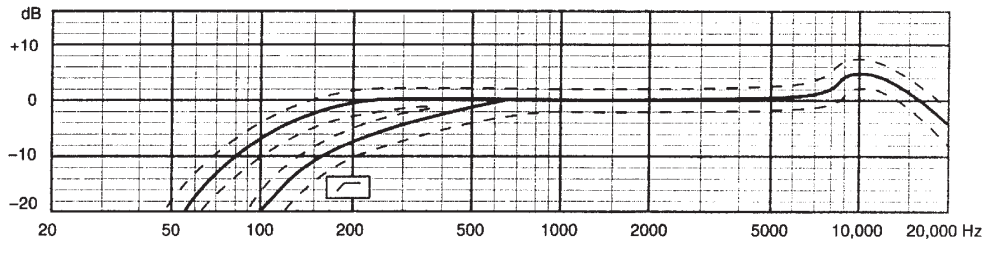
\includegraphics[width=1\textwidth]{resources/images/030-theoretical_framework/Framework_microphone_frequency_response.png}
        \smallcaption{Source: \textcite{Rayburn2004}, page 106}
        \label{fig:frmwk_microphone_frequency_response}
\end{figure}

\subsection{Human hearing capabilities}
\label{subsec:microphones_Human_hearing_capabilities}

The range of sound intensity (pressure) and frequency to which the ear responds is truly astonishing as presented in Figure \ref{fig:frmwk_microphone_human_hearing} below. The intensity ratio between painful noises and the weakest sounds humans can hear is greater than $10^{12}$ and the frequency ratio between the highest and lowest frequencies humans can hear is roughly 1,000 times greater (20 \gls{hz} and as high as 20,000 \gls{hz}), or more than nine octaves - each octave represents a frequency doubling \cite{Rossing2013}. The auditory system's selectivity is another noteworthy feature, and also according to \textcite{Rossing2013}, a listener can discern the sound of a solo instrument among the blended sounds of a symphony orchestra, it is possible to distinguish a single speaker in a crowded room, a mother's conditioned ear can respond to an infant's cry even while she is sleeping and one may even teach himself to sleep through city traffic noise but wake up at the sound of an alarm clock or odd noise.

In general, the frequency response of the human ear is highest in the range of 2-4 \gls{k}\gls{hz} and gradually decreases at higher and lower frequencies as illustrated in the Figure \ref{fig:frmwk_microphone_human_hearing} by the curves threshold of pain and threshold of audibility \cite{Moore2013}.

\begin{figure}[htbp]
    \raggedright
        \caption{Range of frequencies and intensities to which the auditory system (ear) responds.}
        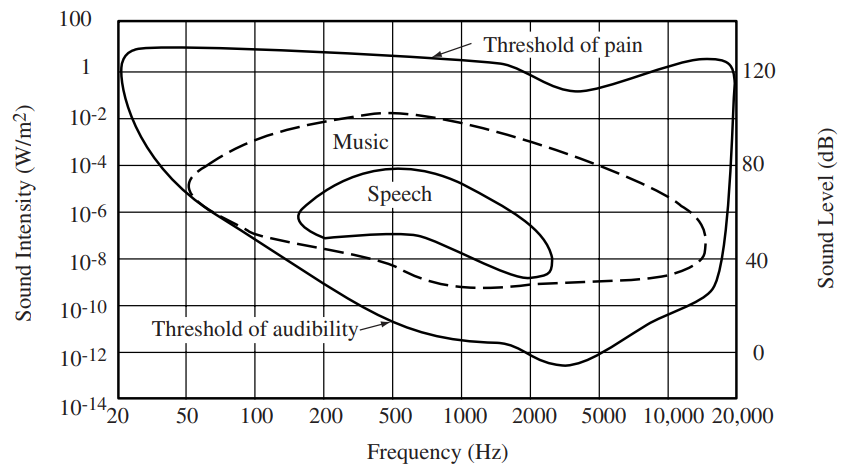
\includegraphics[width=1\textwidth]{resources/images/030-theoretical_framework/Framework_microphone_human_hearing.png}
        \smallcaption{Source: \textcite{Rossing2013}, page 80}
        \label{fig:frmwk_microphone_human_hearing}
\end{figure}


\subsection{Automotive vehicle microphones}
\label{subsec:microphones_automotive_vehicle}

There is a relatively small body of literature that is directly related to the types of microphones commonly used in regular passenger cars. In general, they are used in automotive vehicles for a variety of purposes, including hands-free calling, voice-activated controls, and in-car entertainment systems \cite{Newcomb2008}. The ones listed below are the microphone types commonly used in regular passenger cars according to \textcite{Rumreich2005}:

\begin{itemize}
    \item Built-in microphones: many modern vehicles come with built-in microphones that are integrated into the dashboard or ceiling of the cabin. These microphones are often used for hands-free calling and voice-activated controls, and are typically designed to pick up sound from within the cabin;
    \item Headset microphones: some vehicles come with headsets that have built-in microphones, which can be worn by the driver or passengers to communicate with other passengers or with the vehicle's audio system. These microphones are typically small and lightweight, and are designed to be comfortable to wear for extended periods;
    \item External microphones: in some cases, external microphones may be used in automotive vehicles to pick up sound from outside the cabin, such as when using a hands-free calling system while driving with the windows down. These microphones are typically designed to be weather-resistant and durable, and may be mounted on the vehicle's exterior;
    \item Bluetooth microphones: many modern vehicles are equipped with Bluetooth technology, which allows users to connect their smartphones or other devices wirelessly to the vehicle's audio system. Bluetooth microphones are commonly used for hands-free calling and voice-activated controls, and are designed to be small and unobtrusive.
\end{itemize}

Overall, the type of microphone used in a product will depend on the specific application and the design of the product's audio system. There seems to be a trend in the automotive industry to design audio systems using built-in and Bluetooth microphones, however, in some cases, external microphones may be necessary to achieve the desired level of sound quality and clarity \cite{Rayburn2004}.

Built-in microphones are commonly used in the automotive industry as hardware modules that come equipped with interfacing circuitry and connectors. To detect acoustic signals, these microphones use either a single microphone element for voice sensing in hands-free calling or multiple elements for signal sensing including \gls{anc} in the case of beam forming applications. In particular, \gls{ecm} and \gls{mems} microphone elements are widely utilized in automotive microphone modules and are essential in controlling the acoustic performance of the module \cite{Aubauer2001}. The advancements in microphone elements' signal-to-noise ratio and acoustic overload point specifications do not necessarily improve end-users' experience or \gls{si} in an automotive environment. Even when a simulation model is developed to investigate the impact of microphone element sensitivity and phase mismatches on beam forming performance the results show significant dependency on the chosen array processing algorithm \cite{Du2019}. 

\textcite{Du2022} investigated the \gls{si} of hands-free microphones used in vehicle audio systems, measured by a score (\gls{si} score), which is considered an important performance metric and cannot be directly obtained from the microphone datasheet. They categorized the three most common microphone types in the automotive industry:

\begin{itemize}
    \item Omnidirectional with a flat \gls{fr} shape in the full speech band (e.g., 20-14.000 \gls{hz});
    \item Omnidirectional with a rising \gls{fr} shape and a -3 \gls{db} cut-off frequency between 100 and 500 \gls{hz};
    \item Unidirectional (e.g., Cardioid) microphone.   
\end{itemize}

They draw the conclusion based on their experiments that at low background noise levels, there are no noticeable differences in intelligibility among the three microphones. However, in the presence of medium to high-level and non-wind induced noises, the unidirectional or omnidirectional microphone with a rising frequency response shows certain advantages over the omnidirectional microphone with a flat \gls{fr}. On the other hand, in the presence of wind turbulence-induced noises, which are typically at high levels, the unidirectional microphone exhibits the greatest performance degradation.


\subsection{Conclusion}
\label{subsec:microphones_conclusion}

Based on the body of literature investigated, it can be inferred that the maximum attainable sensitivity level of the microphones typically employed in the automotive industry is conventionally constrained by the caliber of the microphone's transducer and the electronic signal processing circuitry employed to analyze the acoustic beam forming and despite exhibiting noteworthy electroacoustic characteristics, they demonstrate limited potential in attaining the discernment and precision achievable by the human auditory system, however, it is imperative to note that these microphone types do exhibit sufficient attributes capable of detecting a substantial range of acoustic events. This inference imparts significant technological insights regarding the use of automotive microphones in environmental sound recognition.


\section{MACHINE LEARNING}
\label{sec:frmwk_machine_learning}

Machine learning plays a crucial role in enabling autonomous systems to acquire knowledge, make informed decisions, and adapt to dynamic environments. Within the context of \gls{esr}, the current literature predominantly focuses on supervised learning for classification tasks due to its effectiveness and practical applicability. However, semi-supervised and reinforcement learning approaches are also present, mostly for audio tagging tasks. 


\subsection{Classification}
\label{subsec:machine_learning_classification}

In a broader definition given by \textcite{Russel2010}, any component of an agent can be improved by learning from data, essentially depending on four major factors: which \textit{component} is to be improved, what \textit{prior knowledge} the agent already has, what \textit{representation} is used for the data and the component, and what \textit{feedback} is available to learn from.

There are three types of feedback that determine the three main types of learning, with one variation that could be classified as the fourth \cite{Russel2010}:

\textbf{Unsupervised learning} is characterized by the absence of explicit feedback or labeled examples during the learning process. Instead, the agent focuses on recognizing patterns and structures within the input data. By detecting and clustering potentially meaningful groups or clusters of input examples, the agent can uncover valuable insights without external guidance or supervision. An example of unsupervised learning in the domain of environmental sound recognition could involve an autonomous taxi agent gradually developing the concept of "good traffic days" and "bad traffic days" based solely on the audio patterns it observes, without being explicitly provided with labeled examples by a teacher.

\textbf{Reinforcement learning} revolves around the use of a series of reinforcements, which can take the form of rewards or punishments, to guide the learning process. The agent learns by interacting with its environment, receiving positive or negative reinforcement signals based on its actions. Through trial and error, the agent determines which actions led to desirable outcomes and which ones resulted in unfavorable consequences, for instance, in the context of an autonomous vehicle, conveying a rewarded thumbs up by the driver on the infotainment display when the agent detects an ambulance approaching from the rear of the vehicle would serve as an affirmative indication that a correct action was taken. It is the responsibility of the agent to determine the most appropriate actions that result in favorable reinforcement.

\textbf{Supervised learning} involves the agent observing pre-existing example input-output pairs to learn a function that maps input to output. In this learning paradigm, a teacher provides labeled examples, where the output is known or provided by an expert. The agent learns to generalize from these examples, acquiring the ability to make predictions or classifications on unseen data. In the context of environmental sound recognition for autonomous vehicles, supervised learning could manifest as the agent learning to associate specific environmental sound patterns with appropriate responses or actions, for instance, recognizing the sound of emergency sirens and responding accordingly.

In \textbf{semi-supervised learning}, the agent is provided with a limited number of labeled examples while also being presented with a vast collection of unlabeled examples. This learning paradigm falls in between supervised and unsupervised learning, as it attempts to make the best use of both labeled and unlabeled data. The labeled examples serve as a guide for the agent to learn a function mapping the inputs to outputs, similar to the supervised learning approach. However, the unlabeled examples pose a challenge as there is no explicit feedback or labels associated with them.

The presence of inaccuracies and uncertainties in the labeled examples adds complexity to the semi-supervised learning process, for example, considering a scenario where the task is to discern between the sound of a siren, animal, or children playing. In this case, individuals imitating these sounds might introduce intentional inaccuracies, thereby adding random noise and systemic errors in the labeled dataset. Resolving and mitigating these inaccuracies would entail an unsupervised learning problem, wherein the system needs to analyze the relationships between the audio samples, the imitated sound sources, and the true (unknown) sound sources, thus both noise and lack of labels create a continuum between supervised and unsupervised learning. There are several approaches for this type of learning, namely the most utilized: self-training, semi-supervised variants of supervised algorithms, graph-based models and generative models.


\subsection{Training process}
\label{subsec:machine_learning_training}

The training process of traditional machine learning algorithms involves the utilization of labeled datasets to facilitate the learning of patterns and associations in the data. These algorithms aim to extract features from the input data and apply statistical methods to model the relationships and make predictions based on the learned patterns. In the context of the learning task defined \cite{Mitchell1997}, which involves the classification of environmental sounds for autonomous vehicles, the training process would entail feeding the algorithm with an annotated dataset of environmental sound recordings along with their corresponding class labels, hence, an explicitly supervised learning. The algorithm would then analyze the input features, such as frequency content or temporal characteristics, and create a model that can classify new incoming sounds based on its learned patterns.


\subsection{Commonly used classification algorithms}
\label{subsec:machine_learning_common_classification}

This section provides an overview of the classifiers examined in this study, starting with the famous \gls{k-nn} , following by \gls{gnb}, \gls{svm}, \gls{lr}, \gls{rf} and a Voting classifier.  Although this selection represents only a small fraction of the classifiers proposed and investigated in existing literature, they serve well to the purpose to focus on selected methods which are both popular and representative among the wealth of techniques that are available. Instead of delving into lengthy theoretical descriptions, this study emphasizes the fundamental concepts underlying the algorithms. Notably, these classifiers have been chosen for experimental and simulation testing in the implementation due to their prevalent usage in the literature, more specifically in \textcite{Bountourakis2015}, \textcite{Silva2019} and \textcite{Lhoest2021}.


\subsubsection{k-Nearest Neighbor (k-NN)}
\label{subsubsec:machine_learning_k-NN}

The concept underlying the \textbf{\gls{k-nn}} classifier is based on the principle of a nonparametric models, also named \textbf{instance-based learning} or \textbf{memory-based learning}, which do not adhere to a predetermined set of parameters but rather utilize the entire training dataset to generate predictions \cite{Russel2010}. 

The basic approach uses as table lookup to store all training examples and retrieve the corresponding output for a given input query, however, table lookup often lacks generalization capabilities and can only provide a default output when a query is not present in the table.

To enhance the table lookup method, the \gls{k-nn} identifies the $k$ examples of a point ($\mathbf{x}_j$) closest to a given query ($\mathbf{x}_q$), counting how many of those belong to each class by employing a plurality vote among the nearest neighbors and odd values of $k$ to avoid ties. The word "closest" entails a distance, and for that, several metrics could be applied, but the most common approach according \textcite{Russel2010} is the \textbf{Minkowski distance} or $L^p$ norm, defined in a multi-dimensional space $D$ as:

\begin{equation}
    \label{eq:minkowski_distance}
L^p\left(\mathbf{x}_j, \mathbf{x}_q\right)=\left(\sum_i^D\left|x_{j, i}-x_{q, i}\right|^p\right)^{1 / p}
\end{equation}

Setting $p=1$ results in the \textbf{Manhattan distance}, more fitting to dissimilar properties such as gender, weight and age of patient. Whereas $p=2$ results in the well-know \textbf{Euclidean distance}, that performs better if the dimensions are measuring similar properties, such as the width, height and depth of parts on a transportation belt.

Let a set of patterns $\mathbf{x}_j$ represents an unknown feature vector, after calculating the numerical distances $L^p\left(\mathbf{x}_j, \mathbf{x}_q\right)$ for each ${x}_q$, the resulting distances are sorted in ascending order. The $k$ closest neighbors of the unknown feature vector are identified as the $k$ first values in the sorted list. Furthermore, let $k_i$ denote the number of training vectors belonging to the $i^{t h}$ class among the $k$ neighbors of the unknown feature vector, where $i$ ranges from 1 to $N_c$. Based on this, the unknown vector is classified into the class that corresponds to the highest value of $k_i$. 

It is important to note that by using the raw numbers from each dimension can lead to a distortion of the total distance calculation due to variations in scale across different dimensions. To avoid this, a simple approach according to \textcite{Hastie2009} is to first standardize each of the properties or features to have mean equals to 0 and variance equals to 1 so that $x_{j, i}$ becomes $\left(x_{j, i}-\mu_i\right) / \sigma_i$.

 In low-dimensional spaces with abundant data, the nearest neighbors approach tends to perform exceptionally well, as a sufficient number of nearby data points are available to achieve accurate results. However, in high-dimensional spaces, an inherent issue arises in which the nearest neighbors are often relatively distant and the amount of data needed to effectively cover the space grows exponentially, rendering their effectiveness diminished. This problem is described as the \textbf{curse of dimensionality} by \textcite{Russel2010}, \textcite{Hastie2009} and it was originally defined by \textcite{Bellman1961}.

Similar to other memory-based learning classifiers, \gls{k-nn} has some advantages though, such as simplicity and flexibility, as it can adapt to new data without the need for retraining the entire model. On the other hand, choosing the appropriate number of nearest neighbors is crucial for the algorithm efficiency. A small $k$ value may cause overfitting, leading the classifier to be overly sensitive to noise. Conversely, a large $k$ value may cause underfitting, resulting in poor generalization of the classifier, therefore, the number of $k$ is typically adjusted through experimentation with the dataset at hand.


\subsubsection{Support Vector Machine (SVM)}
\label{subsubsec:machine_learning_svm}

\textbf{\gls{svm}} is a powerful framework of supervised learning algorithms commonly employed for binary classification tasks, being very popular and recognized for their efficiency in terms of computational cost for prediction and their ability to yield accurate solutions even when training data is scarce. The primary objective of \gls{svm} is to determine the optimal hyperplane in an $N$-dimensional parameter-space $\mathbb{R}^N$ that possesses the maximum margin $M$ between data samples belonging to different classes, facilitating the effective separation of different classes within the feature space \cite{Russel2010}. A simple illustration of this concept is depicted in Figure \ref{fig:frmwk_machine_learning_svm} (a) where some data belonging to a bi-dimensional space, represented by circles and squares, are separated by a straight-bold line, and the margins are defined by the intersection of the solid circles and squares with an offset of the boundary line.

\begin{figure}[htbp]
    \raggedright
        \caption{Classification example of SVM with the maximum margin hyperplane defined by the support vectors represented as filled circles and squares. (a) without soft margin, (b) with soft margin.}
        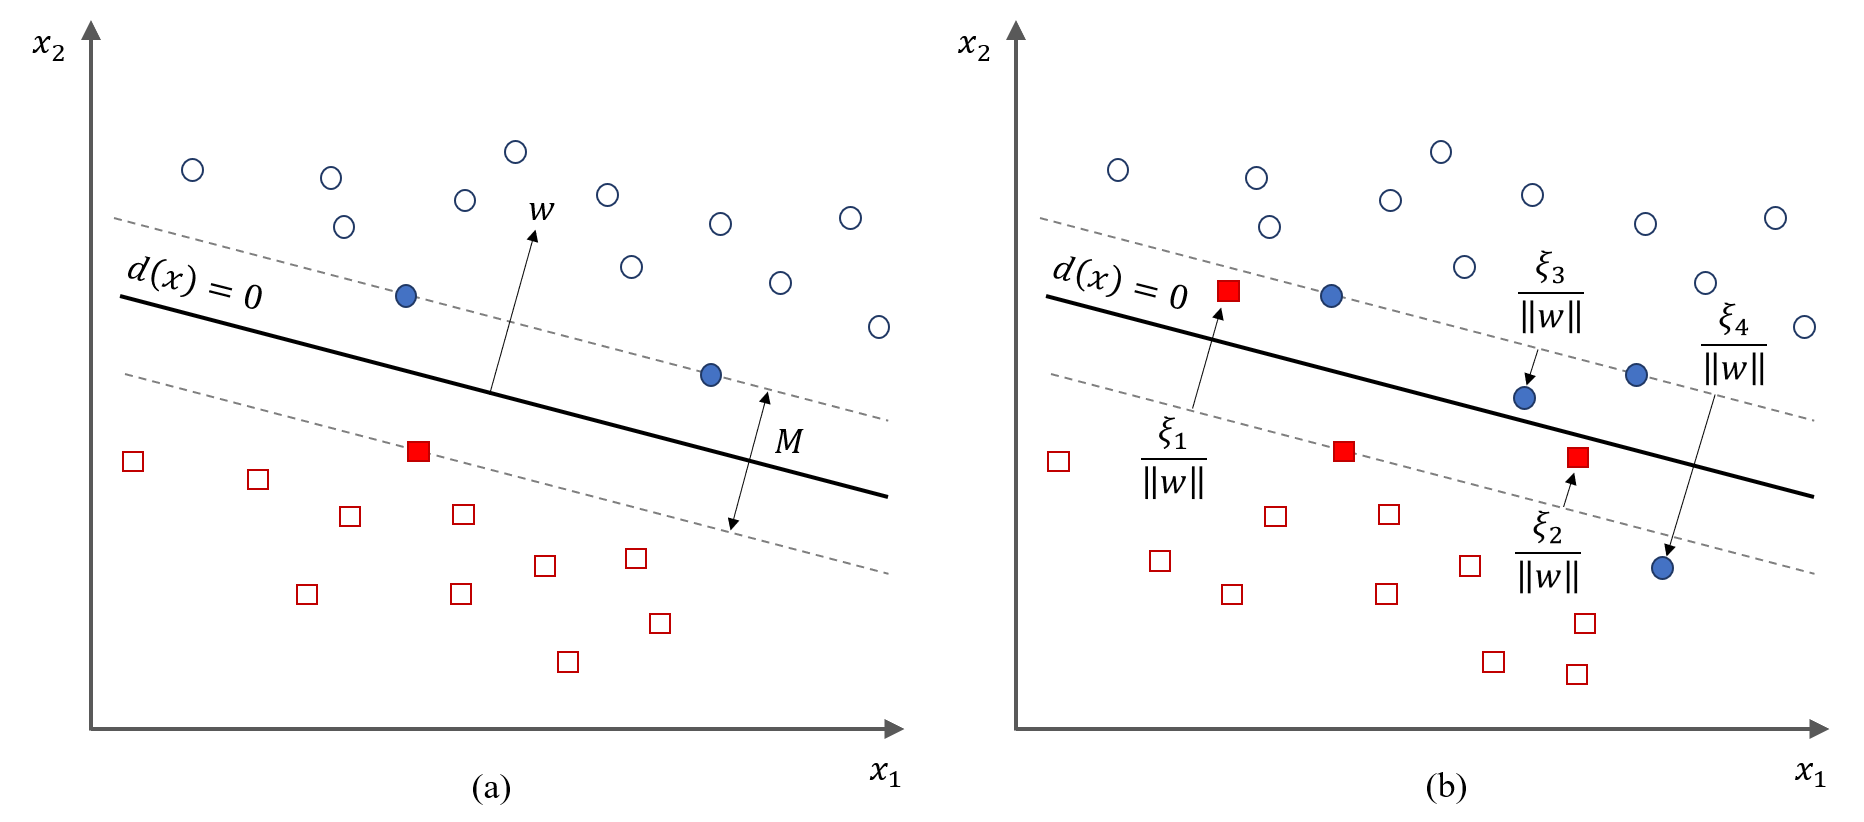
\includegraphics[width=1.0\textwidth]{resources/images/030-theoretical_framework/Framework_machine_learning_SVM.png}
        \smallcaption{Source: Author}
        \label{fig:frmwk_machine_learning_svm}
\end{figure}

In essence, the classification of data points into classes $(y = +1)$ or $(y = -1)$ in a multidimensional space can be accomplished by determining their position in relation to a hyperplane. Specifically, data points located on one side of the hyperplane $(d > 0)$ are associated with one class, whereas those on the other side $(d < 0)$ are attributed to the other class. The weight vector $w$, perpendicular to the hyperplane, determines the orientation of the hyperplane in the multidimensional space $\mathbb{R}^N$, while the bias $w_0$ shifts its position from the origin $\frac{w_0}{\parallel w \parallel}$. To maximize the margin $M$, the constraints are defined given all training examples {$x^{(i)}, y^{(i)}$}.

In practice, it is enough to retain the support vectors $x(i)$ with non-zero weights $\alpha_i$ as illustrated in Figure \ref{fig:frmwk_machine_learning_svm} by the filled circles and squares. Considering the linearity of the decision boundary, standard \gls{svm}s can only classify linearly separable data, however, \gls{svm}s have the ability to embed the data into a higher-dimensional space by applying a non-linear function $\Phi: \mathbb{R}^{N_1} \rightarrow \mathbb{R}^{N_2}$ to the input $x$, converting it to a non-linear space $\mathbb{R}^{N_2} (N_2 > N_1)$, where non-linearly spaced data can be separated using a linear decision function. Figure \ref{fig:frmwk_machine_learning_svm_kernel_trick} depicts this concept, where (a) is a two-dimensional training set with positive examples as black circles and negative examples as white circles. The true decision boundary is defined by the circumference, and (b) is the the same data after mapping into a three-dimensional input space. The circular decision boundary in (a) becomes a linear decision boundary in three dimensions.

\begin{figure}[htbp]
    \raggedright
        \caption{Applying a non-linear transformation $\Phi$ to the input feature space to separate non-linearly spaced data with a linear hyperplane}
        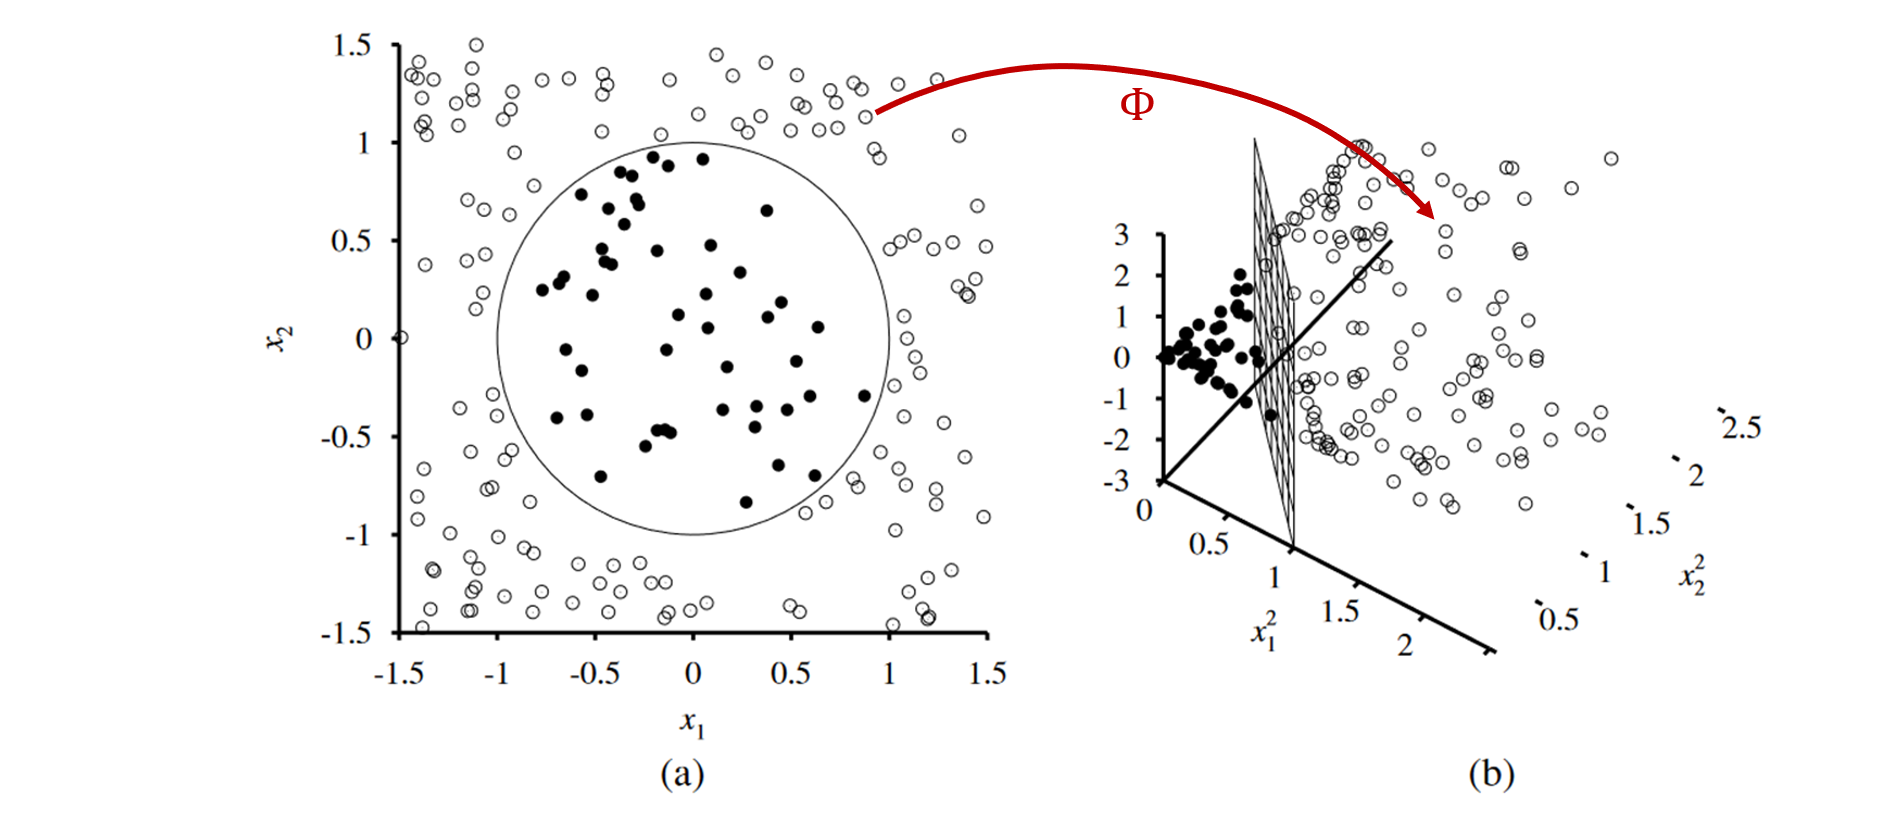
\includegraphics[width=1\textwidth]{resources/images/030-theoretical_framework/Framework_machine_learning_SVM_kernel_trick.png}
        \smallcaption{Source: Author "adapted from" \textcite{Russel2010}, page 747}
        \label{fig:frmwk_machine_learning_svm_kernel_trick}
\end{figure}

At this point, \textcite{Russel2010} highlights that the transformation $\Phi(x)$ to the input data presents significant computational challenges, and in some cases, it may be impracticable (e.g., with infinite $N_2$). However, the so called \textbf{kernel trick} offers a solution by simplifying the transformation to a higher-order feature space through kernel evaluations. 

There are several kernel functions to be plugged in the \gls{svm}s, namely: linear, polynomial, quadratic, and perceptron, but according to \textcite{Goodfellow2016}, the most commonly utilized kernel is the Gaussian kernel, also know as the \textbf{\gls{rbf} kernel}.

When dealing with inherently noisy data, a linear separator in a high-dimensional space might not be desirable. Instead, one seek a decision surface in a lower-dimensional space that acknowledges the lack of clean separation between classes, reflecting the noisy nature of the data. This is achievable with the \textbf{soft margin} classifier, permitting examples to be situated on the incorrect side of the decision boundary while imposing a penalty proportional to the distance needed to relocate them to the correct side \cite{Russel2010}.

According to \textcite{Rothmund2018}, the penalty parameter $C$ essentially regulates the number of support vectors situated within the margin or on the 'wrong' side of the decision function ($\xi_i \neq 0$). When $C$ is small, the decision boundary becomes smoother, reducing the risk of overfitting. Conversely, a larger penalty $C$ results in a more intricate decision boundary that closely represents the training data. The objective is to determine a suitable parameter $C$ that captures the underlying trend in the training data without being excessively complex (leading to overfitting) or overly simplistic (resulting in underfitting). An example of soft margin $\frac{\xi_i}{\parallel w \parallel}$ is depicted in Figure \ref{fig:frmwk_machine_learning_svm} (b) by the filled circles and squares within the margin or even on the wrong side of the decision boundary.

\gls{svm} can be used for \textbf{multi-class discrimination} by combining several \gls{svm}s thus creating a multi-class classifier for $N_c > 2$. Two methods are frequently available in the literatures, the One-vs-Rest and the One-vs-One.

In the \textbf{One-vs-Rest} or \textbf{One-vs-All}, each class $c$ is trained individually, where samples belonging to class $c$ are labeled as positive $(y = 1)$, while the remaining samples are labeled as negative $(y = -1)$. The output class is determined by the maximum output score, such as the distance from the decision boundary.

The \textbf{One-vs-One} approach is more computationally demanding. In this method, $\frac{N_c(N_c-1)}{2}$ binary classifiers are trained, where each classifier corresponds to a unique pair of classes \{$c_i, c_j$\}. The binary output predictions from these classifiers are then aggregated by tallying the number of positive predictions for each class.

Although \gls{svm}s are highly sophisticated, they are not flawless: kernel machines encounter a significant computational burden during training, particularly with large datasets, and generic kernels often struggle to generalize well. According to \textcite{Goodfellow2016}, the modern incarnation of deep learning was designed to overcome these limitations of kernel machines and its very renaissance began when \textcite{Hinton2006} demonstrated that a neural network could outperform the \gls{rbf} kernel \gls{svm} on the MNIST benchmark.


\subsubsection{Naïve Bayes}
\label{subsubsec:machine_learning_GNB}

The naïve Bayes classifier is a supervised machine learning algorithm that uses the principles of probability and Bayes' theorem to perform classification tasks. It is called naïve because it makes two simplifying assumptions: that the features are conditionally independent given the class, and that all features have equal importance. Despite these unrealistic assumptions, the naïve Bayes classifier often works well in practice and is widely used for text classification, spam filtering, sentiment analysis, and more \cite{Barber2012}.

Depending on the choice of distribution, the naïve Bayes classifier can have different variants, such as the Bernoulli naïve Bayes can be used for binary features, the multinomial naïve Bayes can be used for categorical features, and the Gaussian naïve Bayes can be used for continuous features \cite{Friedman1997}. This study implemented the \textbf{\glsdisp{gnb}{Gaussian Naïve Bayes} (\gls{gnb})} algorithm from the Python library scikit-learn.

The naïve Bayes classifier has several advantages and disadvantages. Some of the advantages are that it is easy to implement, fast to train and test, robust to noise and irrelevant features, and scalable to large datasets. Some of the disadvantages are that it can suffer from zero-frequency problems, where a feature value that does not occur in the training data leads to a zero posterior probability, and that it can perform poorly when the independence and equal importance assumptions are violated. To overcome these limitations, various smoothing techniques and feature selection methods can be applied \cite{Wickramasinghe2021}.

As a remark, \gls{glm} is a probabilistic model that assumes all the data points are generated from a mixture of several Gaussian distributions with unknown parameters and \gls{gmm} is a framework for modeling relationships between a response variable and one or more explanatory variables, which includes linear regression, logistic regression, Poisson regression, etc. While they all involve probability and modeling, including \gls{gnb}, they differ in their underlying assumptions, methodologies, and applications.


\subsubsection{Logistic Regression}
\label{subsubsec:machine_learning_logistic_regrassion}

\textbf{\glsdisp{lr}{Logistic Regression} (\gls{lr})} is a statistical method used for binary classification tasks, where the goal is to predict the probability that an instance belongs to one of two classes. Despite its name, logistic regression is a classification algorithm rather than a regression one.

The literature on \gls{lr} model is extensive as evidenced by works such as \cite{Mitchell1997}, \cite{Bouguila2020} and \cite{Russel2010}, therefore it suffices to state the basic idea, where the model applies the logistic function (also known as the sigmoid function) to the linear combination of input features. This function maps any real-valued number to the range between 0 and 1, which makes it suitable for representing probabilities.

\gls{lr} is trained using optimization algorithms, namely some of them: maximum likelihood estimation, gradient descent and limited-memory BFGS, or an online algorithm, such stochastic gradient descent. The training aims to find the optimal values for the coefficients that minimize a cost function, typically the log loss or cross-entropy loss, which measures the difference between the predicted probabilities and the actual class labels in the training data.

\gls{lr} is inherently a binary classification algorithm, however, it can be extended to handle multiclass classification tasks through several strategies, namely:

\begin{itemize}
    \item \textbf{One-vs-Rest} or \textbf{One-vs-All}: by training one classifier per class and treating that class as the positive class, and all other classes as the negative class. During prediction, the class with the highest probability from the individual classifiers is the winner;
    \item \textbf{Multinomial (Softmax)}: it handles multiple classes directly without the need for multiple binary classifiers. Instead of predicting a binary outcome, it predicts the probabilities of each class using the softmax function, which normalizes the output into a probability distribution over multiple classes. During training, it minimizes the cross-entropy loss, which measures the difference between the predicted probabilities and the actual class labels;
    \item \textbf{Multiclass Hinge Loss}: this function penalizes predictions that are not sufficiently correct, aiming to maximize the margin between classes. This approach from \gls{svm} is often used when the emphasis is on maximizing margins between classes rather than directly optimizing probabilities.
\end{itemize}

This algorithm offers simplicity and interpretability, and furthermore, it has computational efficiency and resistance to overfitting, especially with smaller datasets. However, logistic regression assumes a linear relationship between features and outcomes, limiting its ability to capture complex patterns in the data. It struggles with non-linear relationships, large feature spaces, and outliers, which can affect its performance adversely \cite{Russel2010}.


\subsubsection{Random Forest (RF)}
\label{subsubsec:machine_learning_random_forest}

\textbf{\glsdisp{rf}{Random Forest} (\gls{rf})} is a popular ensemble learning method in machine learning. It's essentially a collection of decision trees, where each tree is trained on a different subset of the training data, and the final prediction is made by averaging (for regression) or voting (for classification) the predictions of all the individual trees. The method has essentially the following steps below according to \textcite{Breiman2001}, \textcite{Hartshorn2016} and \textcite{Genuer2020}:

\textbf{Bootstrap sampling}: \gls{rf} builds multiple decision trees based on random subsets of the training data. This sampling technique, known as bootstrap sampling, involves selecting $k$ random samples with replacement from the original dataset, notably, some instances may appear multiple times in a subset, while others may not appear at all. Theoretically, $k$ samples will cover 2/3 of the original dataset, while the rest is called Out-Of-Bag.

\textbf{Feature randomness and decision tree construction}: When building each decision tree, \gls{rf} also introduces randomness in the features that can be considered at each split. Instead of considering all features at every split, it randomly selects a subset of $m$ features from $M$ total features and chooses the best split from that subset. This helps to decorrelate the trees, making them more diverse and less likely to overfit the training data. It is recommended to start with $m = \sqrt{M}$ number of selected features and then reduce or increase $m$ value until the minimum error for the Out-Of-Bag dataset is achieved. The best split is determined by assessing its quality using metrics from the "information theory" such as Gini impurity or entropy.

\textbf{Voting} or averaging for predictions: Once all the trees are constructed, predictions are made for new instances by each individual tree. For regression tasks, the final prediction is usually the average of the predictions of all trees, whereas for classification tasks, the final prediction is determined by majority voting among all trees.

According to \textcite{Genuer2020}, \gls{rf} is among the preferred methods in the toolbox of statisticians and other data scientists due to its high accuracy, robustness to noise and irrelevant features, and ability to handle large datasets. It is also relatively easy to use and requires minimal parameter tuning, however, it can be computationally expensive and may not perform well on imbalanced datasets.


\subsubsection{Voting classifier}
\label{subsubsec:machine_learning_voting_classifer}

Voting classifier, also known as a probabilistic voting classifier, is an ensemble learning method in machine learning that combines multiple base classifiers and predicts the class label based on the probabilities of each class output by the individual classifiers.

Each base classifier in the ensemble independently predicts the class label for a given input. Instead of directly taking a majority vote, the voting classifier calculates the probabilities assigned to each class label by each base classifier, then it averages these probabilities for each class across all the base classifiers, and finally, the class label with the highest average probability is chosen as the final prediction \cite{Sarkar2019}.

This approach is particularly effective when the base classifiers are capable of providing probability estimates for their predictions, such as in the case of many classification algorithms like \gls{lr}, \gls{svm}s with probability outputs, or decision trees with probability outputs.

There are two types of voting classifiers: hard voting and soft voting. In hard voting, the final prediction is the class that receives the most votes from the individual models. In soft voting, the final prediction is the class with the highest average probability across all the individual models. Soft voting typically outperforms hard voting (where the majority vote is taken directly) because it considers the confidence levels of individual classifiers, resulting in more nuanced and often more accurate predictions.

According to \textcite{Sarkar2019}, this ensemble technique is robust against overfitting and outliers, as it averages out individual errors and biases. However, voting classifiers can be computationally intensive, especially when using a large number of diverse base classifiers. Additionally, interpretability may be compromised compared to single-model approaches like \gls{lr}, as the decision-making process involves multiple models. Nonetheless, voting classifiers are highly flexible and effective in a wide range of classification tasks, particularly when the individual base classifiers complement each other's strengths and weaknesses.


\subsection{Conclusion}
\label{subsec:machine_learning_conclusion}

The comprehensive analysis of the machine learning classifiers described in this section highlighted key strengths and weaknesses of them with common themes including considerations such as computational efficiency, generalization capability, robustness to noise, scalability to large datasets, and ease of implementation. Additionally, the trade-offs between model complexity and interpretability are evident across different classifiers. While some of them excel in specific aspects like adaptability to new data \gls{k-nn}, others prioritize accuracy and robustness (\gls{rf}). Moreover, challenges such as overfitting, computational burden, and assumptions violations are recurrent issues that need to be addressed when selecting an appropriate classifier for \gls{esr} tasks. 


\section{NEURAL NETWORKS}
\label{sec:frmwk_neural_networks}

 Neural network, as initially proposed by psychologist Frank Rosenblatt, can be defined as a computational model inspired by the structure and function of the human brain, composed of interconnected artificial neurons, organized in layers, each responsible for performing specific computational tasks. These networks are capable of approximating complex non-linear relationships between inputs and outputs through a process called training, where the network adjusts its internal weights based on a given set of example data. This adaptive learning enables neural networks to recognize patterns, make predictions, and solve various types of problems \cite{Rosenblatt1958}.
 

\subsection{Artificial Neural Network (ANN)}
\label{subsec:neural_network_ANN}

The cornerstone of \gls{ann} lies in a fundamental mathematical model of an artificial neuron introduced by McCulloch-Pitts in 1943. This model serves as the groundwork for computational methodologies in the realm of learning, describing the properties of a single neuron by forming a linear combination of the outputs of other neurons, which is then transformed using a nonlinear function \cite{Bishop2023}. An artificial neuron aggregates the input values {$x_1, x_2, \ldots , x_M$} through a linear combination process illustrated by Figure \ref{fig:frmwk_ann_artificial_neuron} (a). Each input $x_i$ is assigned a weight $w_i$, which is used to scale or weight the input value. The total of the weighted inputs, along with the bias $b$, is defined as the activation $a$, and after it passed through a non-linear activation function $\sigma(a)$, it produces the output state $y_j$ of the neuron. 

\begin{equation}
    \label{eq:ann_activation}
    a = \sum_{i=1}^M w_i \cdot x_i + b \quad\quad y_j = \sigma(a)
\end{equation}

This linear combination cab be expressed by the dot product of a weighted vector $W$ and the input vector $X$, given by:

\begin{equation}
    \label{eq:ann_activation_outpu}
    y_j = \sigma  \left( W^TX +b \right)
\end{equation}

The trainable weight vector $w$ plays a crucial role in determining the significance of an input to a neuron's output. Similarly, the trainable bias $b$ sets the operational point within the non-linear activation function $\sigma(a)$. The activation function $\sigma(a)$ mimics its biological counterpart by limiting the strength of electrical spikes traveling through the axon to a certain range as illustrated in Figure \ref{fig:frmwk_ann_artificial_neuron} (b).

According to \textcite{Bishop2023}, frequently utilized general-purpose non-linear activation functions to constrain the neuron's state $y$ within a reasonable range include hyperbolic tangent (Tanh) and \gls{relu}. Sigmoid and softmax are commonly employed at the neural network's output layer for classification tasks, transforming the input into a probability-like range between 0 and 1 as shown in Figure \ref{fig:frmwk_ann_activation_functions} (a) to (d). Specifically, sigmoid is suitable for binary classification, while softmax performs better for multi-class classification scenarios. in both cases, they are preferred for their regularization benefits and faster training compared to hyperbolic tangent activations. To obtain a discrete class from these continuous probability outputs, a decision function is typically implemented. In single-label multi-class classification, the argmax function is commonly used to select the class with the highest probability value. 

\begin{figure}[htbp]
    \raggedright
        \caption{Artificial neuron mimicking a biological neuron}
        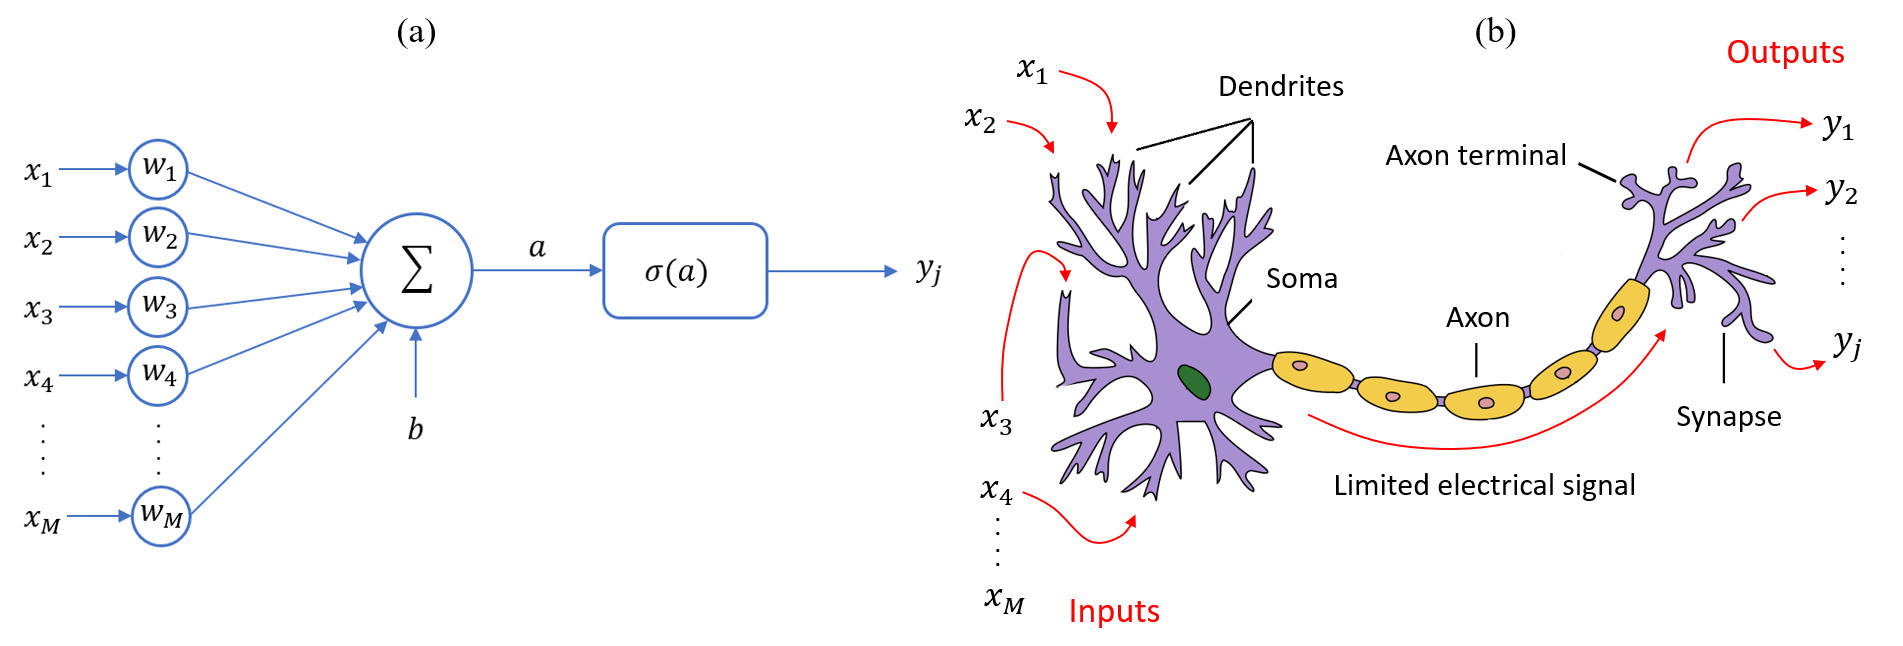
\includegraphics[width=1\textwidth]{resources/images/030-theoretical_framework/Framework_ann_neuron.png}
        \smallcaption{Source: Author}
        \label{fig:frmwk_ann_artificial_neuron}
\end{figure}

\begin{figure}[htbp]
    \raggedright
        \caption{Common activation functions}
        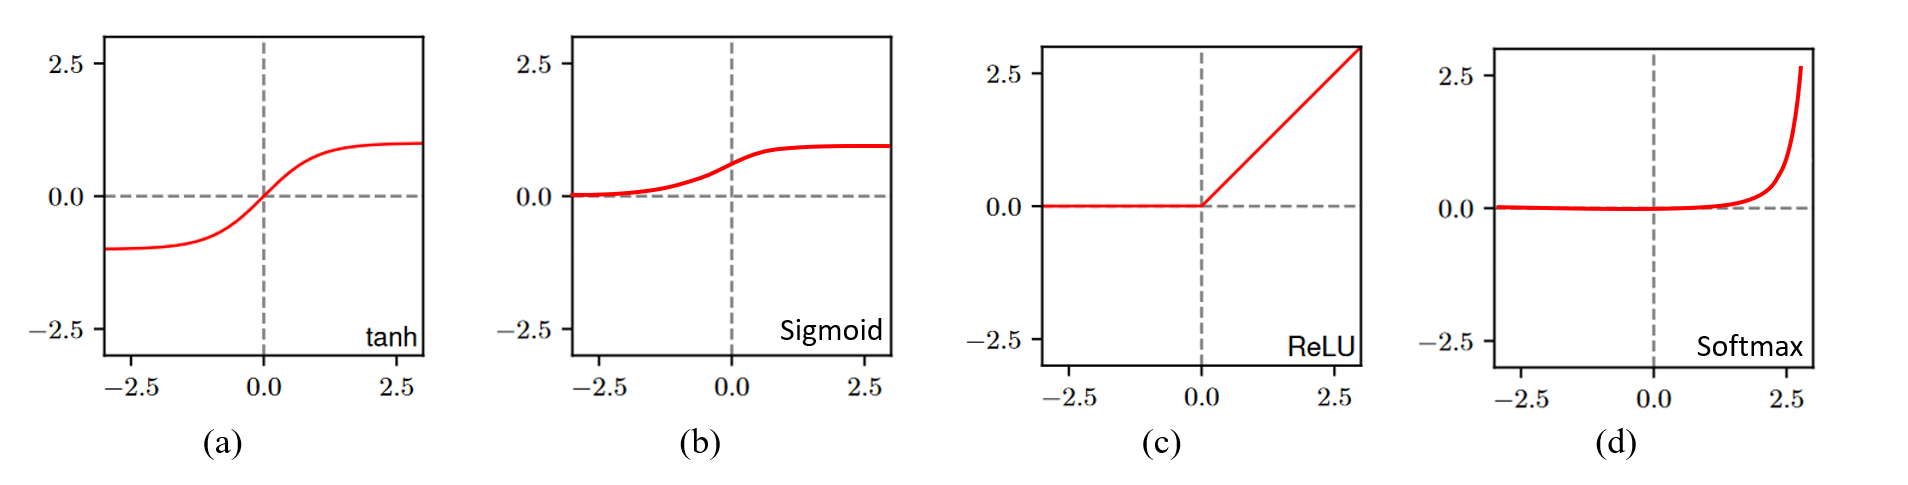
\includegraphics[width=1\textwidth]{resources/images/030-theoretical_framework/Framework_ann_activation_function.png}
        \smallcaption{Source: Author "adapted from" \textcite{Bishop2023}, page 184}
        \label{fig:frmwk_ann_activation_functions}
\end{figure}

One of the most popular \gls{ann} is the \textbf{\gls{mlp}}, a feedforward neural network model that consists of multiple layers of nodes (neurons), each layer fully connected to the next layer, organized consecutively as input, hidden and output layer as depicted in Figure \ref{fig:frmwk_ann_mlp}. The \gls{mlp} is characterized by its ability to learn nonlinear models by using an activation function that introduces non-linearity into the network's decision-making process \cite{Mitchell1997}.

According to \textcite{Russel2010}, the first layer, or the input layer, receives input data features where each node represents a feature of the input data. Followed by hidden layers $L$ that are the intermediate layers between the input and output layers where each node in a hidden layer $l$ consisting of $m^{(l)}$ parallel nodes receives input from all the nodes in the previous layer and applies an activation function $\sigma^{(l)}(a_i^{(l)})$ to the weighted sum of those inputs and fed to the inputs of the next layer ($l+1$). The last layer, or output layer ($L+1$), produces the network output vector. The number of nodes in this layer depends on the problem type, for instance, for binary classification, one might have one output node representing the probability of belonging to one class, and its complement representing the probability of belonging to the other class. 

\gls{mlp}s are trained using supervised learning methods like backpropagation, where the network adjusts its internal parameters (weights and biases) iteratively to minimize the difference between its output and the desired output for a given set of input data. %Similar as in machine learning, training the \gls{ann} is essential to obtain the expected outcome. 
The training process undergo by optimizing a specified objective function, also known as a loss function. In the context of supervised learning, the predominant technique utilized is mini-batch \textbf{\gls{sgd}} coupled with \textbf{Backpropagation}, particularly for classification tasks, the cross-entropy function, commonly referred to as log-loss, is frequently employed. The log-loss function exhibits a tendency towards infinity as the predicted probability of the true class approaches zero %(Figure \ref{fig:frmwk_ann_log_loss})
, imposing significant penalties for wrong predictions. \textbf{Categorical cross-entropy} serves as an extension of binary cross-entropy tailored for scenarios involving multi-class, and according to the problem and the classification tasks, the literature provides additional loss functions such as Logistic Loss, Mean Squared Error, and Mean Absolute Error. The process of generating predictions through a feedforward neural network and subsequently evaluating the loss function facilitates the assessment of the model's performance, and to enhance it, an optimization algorithm is applied to determine necessary adjustments to the model parameters. There are several options for the optimization algorithm such as \gls{sgd}, Adam, RMSprop, etc, but they all generate a gradient of a function that quantifies the rate and direction of its output variations in response to incremental modifications in its inputs, computed through partial derivatives of the function \cite{Bishop2023}. 

\begin{figure}[htbp]
    \raggedright
        \caption{MLP with $M$ inputs, $L$ hidden layers, each with $m^{(l)}$ nodes and $N_c = 3$ output nodes. Arrows represent weighted connections between nodes}
        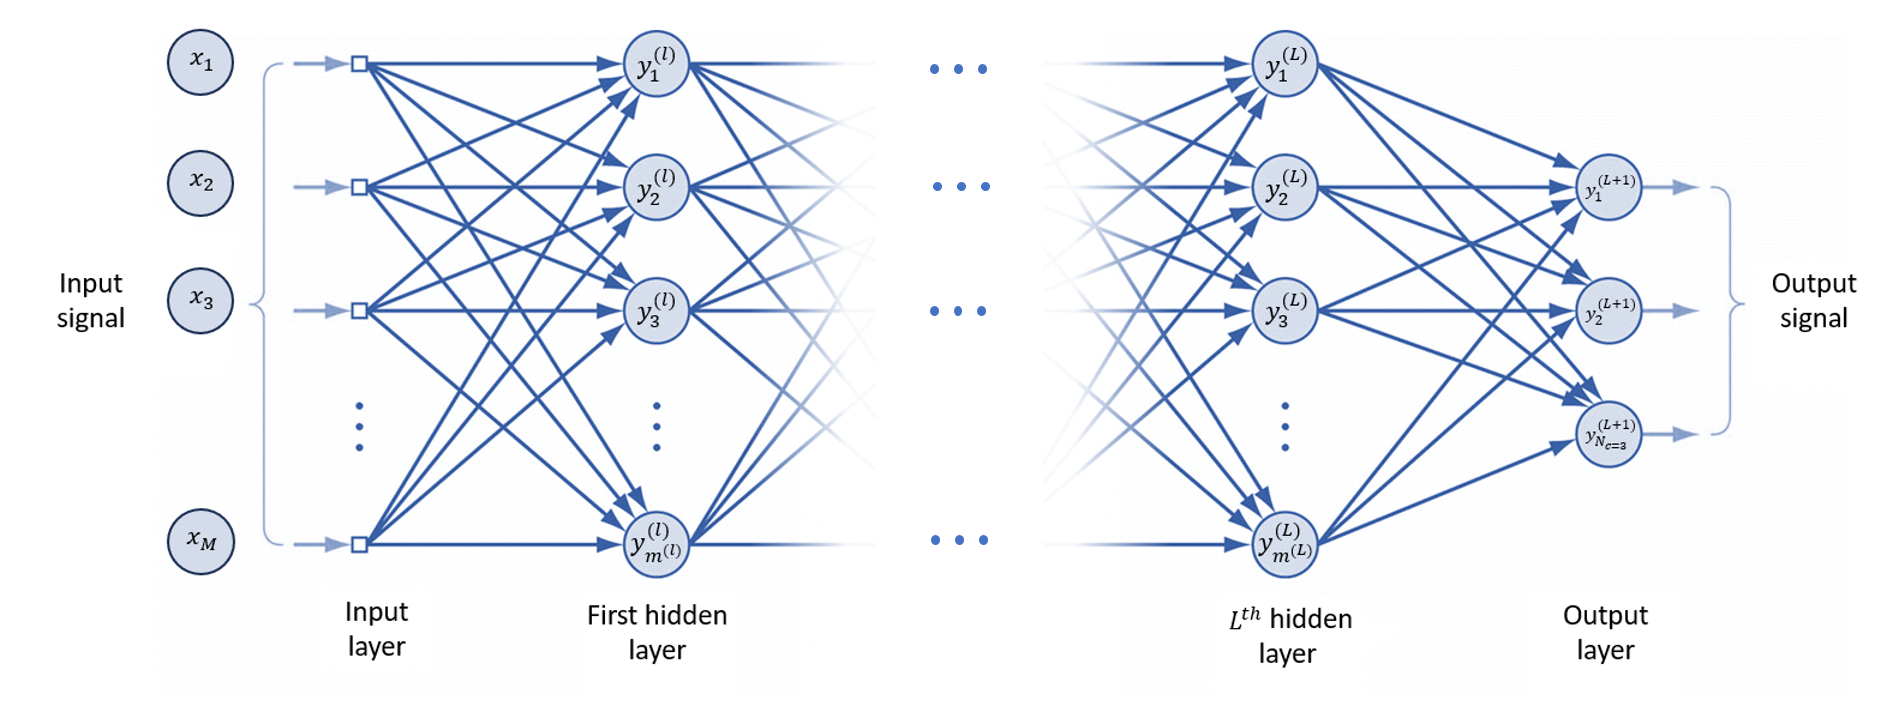
\includegraphics[width=1\textwidth]{resources/images/030-theoretical_framework/Framework_ann_mlp.png}
        \smallcaption{Source: Author}
        \label{fig:frmwk_ann_mlp}
\end{figure}

The fundamental mechanism for computing gradients in a \gls{mlp} is through the utilization of backpropagation \cite{Rumelhart1986}, which involves iteratively propagating the error signals from the output layer back to the input layer by calculating the partial derivatives with respect to the inputs from the preceding layer. This process enables the determination of gradients for each weight and each biases in the network, and subsequently, once the gradients are obtained, weight adjustments are made by moving in the opposite direction of the gradient. To control the magnitude of this adjustment, each step of this process is scaled by a \index{hyperparameter}hyperparameter known as the \textbf{learning rate}, which typically falls within the range of $10^{-7}$ to $10^{-2}$. Selecting an appropriate learning rate is crucial as excessively small values may lead to convergence issues, or local minima, whereas excessively large values can hinder training convergence. There are no shortcuts in this process, and the "rule of thumb" for defining the learning rate is to assess the model results using cross-validation, a systematic and rigorous technique for evaluating the performance of a learning model and for selecting the best hyperparameters.

Optimization algorithms that utilize the complete training set for updating each parameter is referred to as batch training or deterministic gradient methods, where the batch size is equivalent to the total number of observations in the training set. In \textbf{mini-batch} Gradient Descent, the training set is divided into fixed-size batches, and the loss function and model parameter updates are calculated for each batch, allowing for processing large datasets without the need to store all the training data in memory simultaneously. The batch size, a hyperparameter, must be chosen carefully to ensure that the batch loss provides a reasonable approximation of the overall training set loss while still fitting into memory \cite{Bishop2023}. Each complete iteration through the entire training dataset is referred to as an \textbf{epoch}, with multiple epochs typically being conducted during training. 

While Gradient Descent does not ensure discovery of a globally optimal minimum, appropriate hyperparameter selections typically lead to satisfactory local minima. According to \textcite{Choromanska2014}, achieving a global optimum on the training set may not be advantageous, as it is unlikely to result in strong generalized model.


\subsection{Convolutional Neural Network (CNN)}
\label{subsec:convolutional_neural_network_CNN}

\gls{cnn}, as introduced by \textcite{Lecun1998}, is a specialized type of neural network designed for processing data with a structured, grid-like topology, and it has demonstrated significant success in real-world applications. This can include various forms of data such as time-series data represented as a 1D grid with samples taken at regular intervals, and image data represented as a 2D grid of pixels. The term "convolutional neural network" reflects the utilization of the mathematical process known as convolution, which is a specialized form of linear operation within the network architecture. \textcite{Goodfellow2016} defined convolutional network as a simple neural network that uses convolution in place of general matrix multiplication in at least one of its layers.

Essentially, \gls{cnn}s are complex architectures comprised of multiple convolutional layers, followed by pooling/down-sampling layers, and fully-connected layers of artificial neurons. The primary function of convolutional layers is to correlate segments of input data with pre-trained filter kernels to identify patterns, resulting in a high output score for matching features. By incorporating additional convolutional layers, increasingly intricate patterns can be extracted from the input data. Figure \ref{fig:frmwk_cnn_LeNet-5} illustrates the architecture of a \gls{cnn} with two convolutional layers, pooling layers, and fully-connected layers serving as a classifier as proposed by Lecun in the LeNet-5.

\begin{figure}[htbp]
    \raggedright
        \caption{Example of CNN (LeNet-5) proposed by LeCun}
        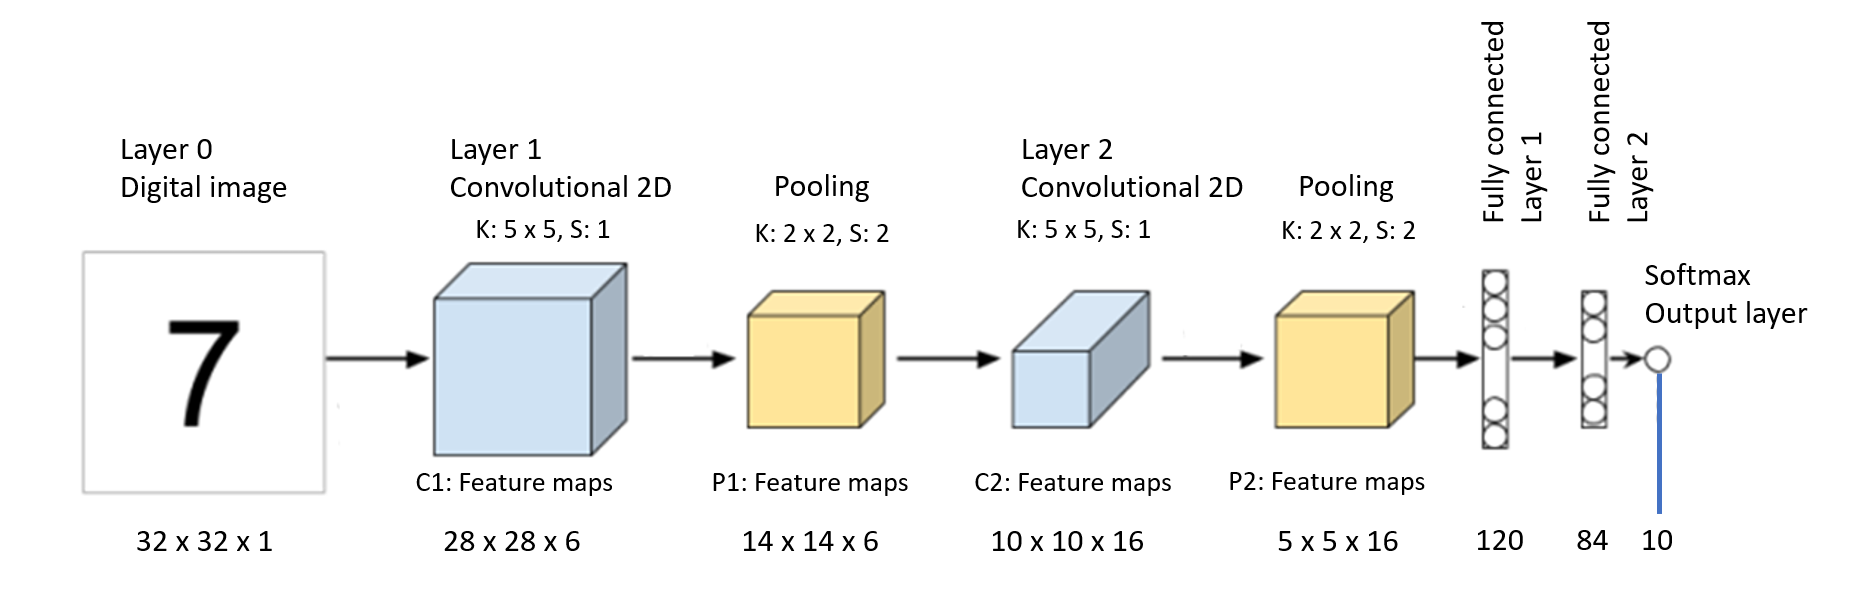
\includegraphics[width=1\textwidth]{resources/images/030-theoretical_framework/Framework_cnn_LeNet-5.png}
        \smallcaption{Source: Author "adapted from" \textcite{Lecun1998}, page 2283}
        \label{fig:frmwk_cnn_LeNet-5}
\end{figure}

According \textcite{Goodfellow2016} and \textcite{Rothmund2018}, the convolution operation is typically denoted with an asterisk (*), and a discrete convolution for functions $x(t)$ and $k(t)$ is expressed as:

\begin{equation}
    \label{eq:cnn_discrete_convolution}
    s(t) = (x * k)(t) = \int x(\tau)k(t-\tau)d\tau
\end{equation}

Given that $x$ and $k$ are defined solely at discrete intervals, the discrete convolution, denoted as $s_i$, can be defined as:

\begin{equation}
    \label{eq:cnn_discrete_convolution_si}
    s_i = (x * k)_i = \sum_{n=-\infty}^{\infty} x_i \cdot k_{i-n} 
\end{equation}

Filter kernels may vary in dimensionality, being one-dimensional, two-dimensional, or three-dimensional, depending on the format of the input data. In the context of image recognition, the convolution process enables the representation of various beneficial transformations on two-dimensional data through the selection of different weights within the kernel. Examples include edge detection (horizontal, vertical, diagonal) and smoothing filters (mean, Gaussian). As the weights of the kernels in a convolutional layer are trained, they become adept at identifying local features specific to the training dataset. In cases involving multiple input channels, a single kernel is applied across all input channels, with the results at a given location and the bias being aggregated to generate the output \cite{Bishop2023}. 

Given a two-dimensional kernel $K$ with dimensions $h_1$ × $h_2$ and an input image $X$ with dimensions $m_1$ × $m_2$, the convolution operation can be expressed according to \textcite{Rothmund2018} as:

\begin{equation}
    \label{eq:cnn_convolution_2D_1}
    s_{i, j}=(X * K)_{i, j}=\sum_{m=1}^{h_1} \sum_{n=1}^{h_2} x_{i-m, j-n} \cdot k_{m, n}
\end{equation}

With input $X$ and the kernel $K$ yielding the two-dimensional output $S$.

\begin{equation}
    \label{eq:cnn_convolution_2D_2}
    K=\left[\begin{array}{llll}
    k_{0,0} & k_{0,1} & \cdots & k_{0, l_2} \\
    k_{1,0} & k_{1,1} & \cdots & k_{1, l_2} \\
    \vdots & \vdots & \ddots & \vdots \\
    k_{l_1, 0} & k_{l_1, 1} & \cdots & k_{l_1, l_2}
    \end{array}\right] \quad \text { and } \quad X=\left[\begin{array}{llll}
    x_{0,0} & x_{0,1} & \cdots & x_{0, m_2} \\
    x_{1,0} & x_{1,1} & \cdots & x_{1, m_2} \\
    \vdots & \vdots & \ddots & \vdots \\
    x_{m_1, 0} & x_{m_1, 1} & \cdots & x_{m_1, m_2}
    \end{array}\right]
\end{equation}

Figure \ref{fig:frmwk_cnn_convolution_example} illustrates the process of a discrete two-dimensional convolution using a small 2×2 kernel designed to detect vertical edges. The kernel is applied to a larger 5×5 dimension input image and computed according to equation \ref{eq:cnn_convolution_2D_1}. The resulting output image highlights the vertical edge with a darker color, while the horizontal edge appears less pronounced. It is important to note that zero-padding was not utilized in this example, leading to a reduction in dimensions for the output image $S$ (4×4). If zero-padding, also named \textit{same padding}, was applied, zeros would be added to the input image's borders in such a way that the output image $S$ would have the same spatial dimensions as the input image $X$.

\begin{figure}[htbp]
    \raggedright
        \caption{2D discrete convolution performed on input image $X$ with dimensions of 5×5 using a filter kernel $K$ with dimensions of 2×2, yielding an output image of size 4×4. The filter kernel is designed to detect and enhance vertical lines in the image.}
        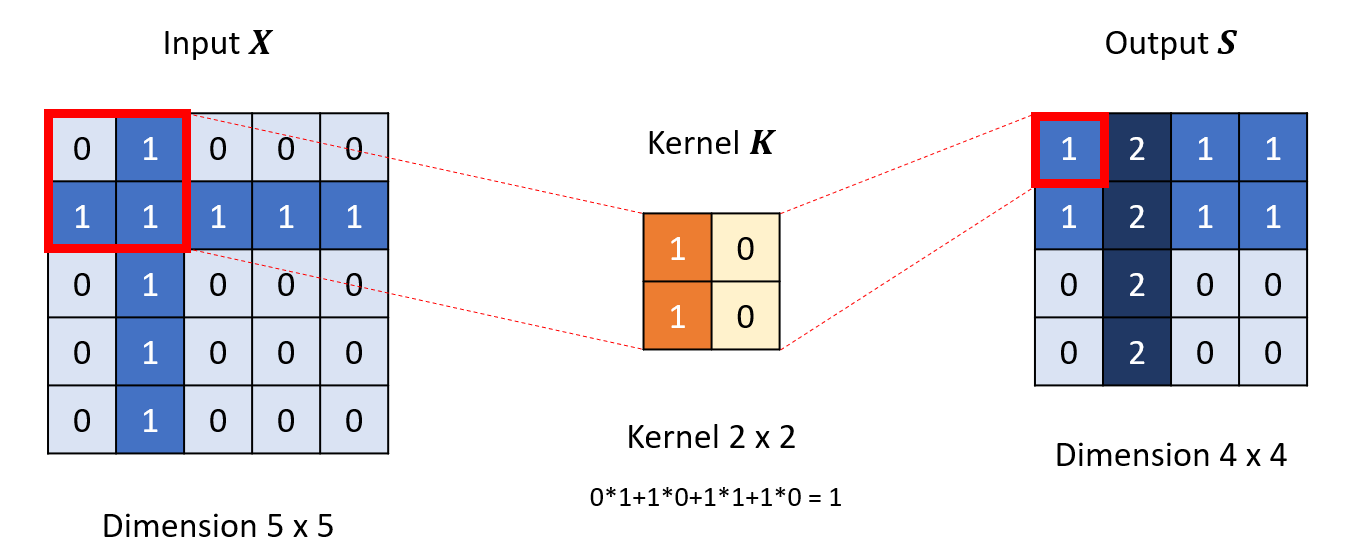
\includegraphics[width=.9\textwidth]{resources/images/030-theoretical_framework/Framework_cnn_example.png}
        \smallcaption{Source: Author}
        \label{fig:frmwk_cnn_convolution_example}
\end{figure}

The input of a two-dimensional \textbf{convolutional layer} $l$ consists of a three-dimensional array containing $n_1^{(l)}$ two-dimensional feature maps with dimensions $n_2^{(l)} \times n_3^{(l)}$. For spectrograms or black and white images, the number of channels or feature maps is denoted as $n_1^{(1)}=1$, while for a colored RGB image (the RGB color space is an additive color model, describing a color in three channels, representing the colors red, green and blue) the number of channels would be $n_1^{(1)}=3$. Each convolutional layer comprises $m_1 \cdot n_1$ filter kernels $K_{i,j}$, each with dimensions $h_1^{(l)} \times h_2^{(l)}$, resulting in $m_1^{(l)}$ two-dimensional feature maps with dimensions $m_1^{(l)} \times m_2^{(l)}$ at the output. These filter kernels, denoted as $K_{i,j}$, are responsible for identifying specific patterns across the input data $X_j$. 

The output feature maps $Y_i^{(l)}$ for layer $l$ are obtained by summing the discrete convolutions of the trainable filter kernels $K_{i,j}$ with the input feature maps $X_j$ and a trainable bias term $b_i^{(l)}$. With $i = 1, 2,\ldots, m_1, j = 1, 2,\ldots, n_1$ and $\sigma^{(l)}$ as the non-linear transformation function, it compute as:

\begin{equation}
    \label{eq:cnn_convolutional_layer}
    Y_i^{(l)}=\sigma^{(l)}\left(b_i^{(l)}+\sum_{j=1}^{n_1^{(l)}} K_{i, j}^{(l)} * X_j^{(l)}\right)
\end{equation}


Subsampling the data as it progresses through the convolutional layers is crucial for enhancing the model's ability to learn larger and more intricate features. This process is achieved through \textbf{pooling layers}, such as the 2D pooling operation with a $f_1$ x $f_2$ sized \textbf{filter} and a \textbf{stride} matching the operation size. Each channel is independently processed in the pooling operation, which outputs either the average value of the input in \textit{average pooling} or the maximum value in \textit{max pooling} as depicted in Figure \ref{fig:frmwk_cnn_pooling}. In other words, pooling layers don't learn any pattern in the network, rather reduce the resolution of the output feature maps from preceding convolutional layers ($Y_i^{(l-1)}$) by applying an filter window of size $f_1$ x $f_2$ with a stride of $s_1$ x $s_2$.

\begin{figure}[htbp]
    \raggedright
        \caption{Pooling examples on a two-dimensional input image $X$ of size $m_1$ × $m_2$ = 4×4 with pool size $f_1$ × $f_2$ = 2×2 and stride $s_1$ × $s_2$ = $f_1$ × $f_2$ (no overlap).}
        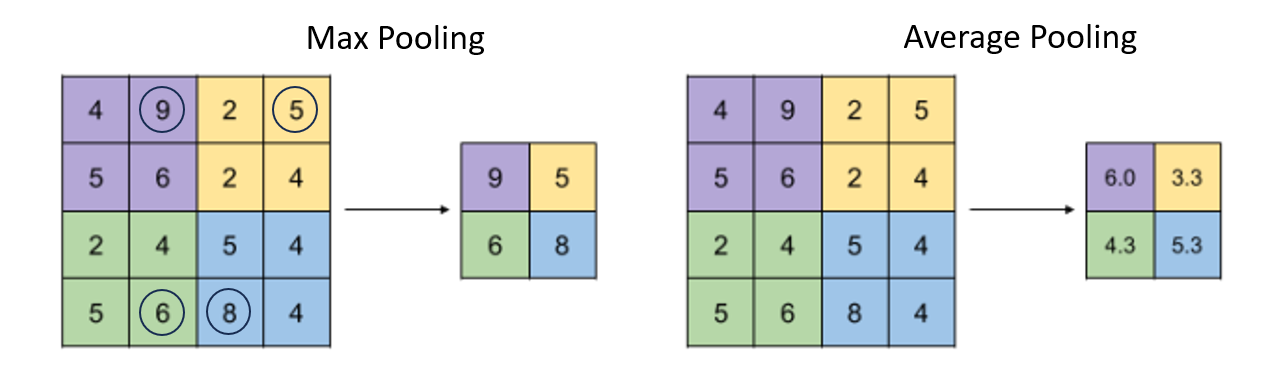
\includegraphics[width=.9\textwidth]{resources/images/030-theoretical_framework/Framework_cnn_pooling.png}
        \smallcaption{Source: Author "adapted from" \textcite{IndoML2018}}
        \label{fig:frmwk_cnn_pooling}
\end{figure}

As a remark, \gls{lstm} networks have recently emerged as a promising alternative to \gls{cnn}s in the field of environmental sound recognition. Unlike \gls{cnn}s which are primarily designed for image processing tasks, \gls{lstm}s are well-suited for sequential data analysis due to their ability to capture long-range dependencies and temporal dynamics in audio signals \cite{Bubashait2021}. By modeling the temporal relationships within sound sequences, \gls{lstm}s can effectively learn intricate patterns and nuances in acoustic data, making them a valuable tool to be further investigated for tasks in the field of \gls{esr}.


\subsection{Conclusion}
\label{sec:frmwk_neural_networks_conclusion}

In the context of \gls{esr}, neural networks are able to offer distinct advantages. \gls{mlp}s provide a strong foundation for understanding basic sound patterns and relationships using the interconnection of hidden layers and neurons, while \gls{cnn} 1D excels in capturing temporal dependencies within sound data. On the other hand, \gls{cnn} 2D is particularly effective in extracting spatial features from spectrogram representations of environmental sounds. By leveraging the unique strengths of each model, a more robust and accurate \gls{esr} algorithm can be developed for autonomous vehicles.


\section{ELECTRONIC CONTROL UNIT}
\label{sec:frmwk_electronic_control_unit}

An \glsdisp{ecu}{Electronic Control Unit} (\gls{ecu}), is an embedded system found in automotive electronics that regulates one or more electrical systems or subsystems within a motor vehicle. To address the requirements of these systems and subsystems, a clear trend in the automotive sector involves the growing prevalence of electronic components within vehicles that are vital for controlling the propulsion, chassis, body functions, in-vehicle networks, and driving information systems. Depending on the system, the \gls{ecu} receives an specific acronym, for example: engine control module (ECM), powertrain control module (PCM), transmission control module (TCM), brake control module (BCM or EBCM), central control module (CCM), body control module (BCM), etc. Although colloquially referred to as the car's computer, it is important to note that these \gls{ecu}s are distinct individual computers running \gls{soc}, rather than a single unit \cite{Aptiv2020}.


\subsection{Vehicle EE architecture}
\label{subsec:ECU_common_units_in_market}

This section will present a brief overview about where the \gls{esr} algorithm could be deployed or embedded within the vehicle \gls{ee} architecture considering the findings of \textcite{Zhu2021} and it will not dwell in the intricacies and details of the architecture itself, rather will focus on the application deployment considering a regular passenger car and an autonomous vehicle.

Assuming a \textbf{centralized gateway architecture} with the \gls{esr} algorithm embedded on a specific \gls{ecu} would have the advantage of improve functional safety given that the gateway converts different protocols and regulates network traffic, on the other hand,  the number of \gls{ecu}s have been increasing constantly which lead to more complexity in the gateway and ultimately, it may be harmful for security. A more updated architecture such a \textbf{domain-based} would integrate portions of the \gls{ecu}, containing specific software components thus reducing material cost and weight in manufacturing processes. Additionally, the overhead in the gateway and bottleneck of multiples \gls{ecu}s will be reduced, conversely, the potential downsize are delays that may be introduced between sensors and actuators. \textbf{Zone-base architecture} is currently a trend, and many automakers are developing their future products based on this concept. The main advantage is that the electronic components can be integrated based on their physical location in the vehicle, reducing cabling, especially for Ethernet, with the combination of communication and power. The disadvantage is that the architecture entails higher requirements for software platforms owing to the location cluster.

Shifting to autonomous vehicles, it is a "common sense" that Tesla is on the vanguard of hardware and software development, and according to \textcite{Lindholm2008}, the underlying structure of the Tesla architecture relies on a flexible processor array based on the GeForce 8800 \gls{gpu}, with 128 streaming-processor (SP) cores, organized into 16 streaming multiprocessors (SMs) that are further grouped into eight separate processing units referred to as texture/processor clusters (TPCs). Notably, this is just a small part of the so called HW4 infotainment system hacked by \textcite{Teslanorth2023} on the Tesla Model. For obvious reasons, Tesla does not disclaim their infotainment technical specifications and therefore, the information that the HW4 infotainment system has 128 \gls{g}\gls{b} of storage capacity and 8 \gls{g}\gls{b} of \gls{ram} is assumed as valid.

The Tesla architecture, developed by NVIDIA, is considered to be the pioneering platform for ubiquitous supercomputing. Its success is attributed to its compatibility with C programming language and the CUDA software development environment, which allows for the efficient deployment of computationally intensive parallel-computing and graphics applications. As transistors become more densely packed in the future, this architecture will be able to effortlessly scale processor parallelism, memory partitions, and overall performance \cite{Lindholm2008}. Based on this conclusion, it is plausible to assume that \gls{esr} algorithms could be deployed in autonomous vehicles using only embedded software in the current \gls{ee} architecture. This approach would bring added value, but not extra costs on hardware. It may be necessary to considered additional sensors like external microphone arrays though.


\subsection{High-end general-purpose embedded platform}
\label{subsec:ECU_high-end-platform}

In the realm of computing, specialized architectures and general-purpose platforms play distinct roles in catering to various computational needs. \glsdisp{fpga}{Field-Programmable Gate Arrays} (\gls{fpga}) and \glsdisp{tpu}{Tensor Processing Units} (\gls{tpu}) are examples of specialized architectures tailored for accelerating machine learning tasks, particularly those involving tensor operations. On the other hand, high-end general-purpose platforms like Raspberry Pi offer versatile computing capabilities at a more accessible price point. Considering the current platform utilized in the C-Bot, this study will focus on the high-end general-purpose platform Raspberry Pi 4, model B \cite{Raspberry2023}, however, this section will briefly explain the most common architectures for machine learning tasks, given that \gls{ecu}s for the automotive industry, specially the ones designed for autonomous vehicles, can have a \gls{fpga} or \gls{tpu} technology embedded in its hardware.

\textbf{\gls{fpga}} is a customizable integrated circuit that can be reconfigured after manufacturing, making it highly flexible for various applications, including accelerating specific algorithms and tasks. It is often used in specialized computing tasks, including machine learning acceleration, digital signal processing, and hardware emulation because they offer parallelism and low-latency processing, making them suitable for real-time applications where performance is critical. Latest technologies in \gls{fpga} include Xilinx Versal AI Core series, advancements in high-level synthesis tools for easier programming, integration with high-speed interfaces like PCIe Gen4 for faster data transfer, and the incorporation of hardened IP blocks for common functions, such as memory controllers and DSP blocks \cite{IntelFPGA2024}.

\textbf{\gls{tpu}}s Google's custom-built ASIC (Application-Specific Integrated Circuit) is designed specifically for accelerating machine learning workloads, more specifically, optimized for \index{Tensorflow}TensorFlow \cite{TensorFl23}, Google's open-source machine learning framework, but can also be used with other frameworks like PyTorch and JAX. They excel at both training and inference tasks and are known for their high performance and energy efficiency. Recent advancements in \gls{tpu} technology include the development of second and third-generation \gls{tpu}s, which feature higher computational capabilities, increased memory bandwidth, and improved support for mixed-precision computing (Coral Dev Board). Additionally, there is ongoing research into integrating \gls{tpu}s with Google's Cloud AI infrastructure to provide scalable and efficient machine learning solutions for various industries \cite{GoogleTPU2024}.

\textbf{Raspberry Pi} is a series of small single-board computers developed by the Raspberry Pi Foundation, and although not as powerful or specialized as \gls{fpga} or \gls{tpu}, Raspberry Pi offers a cost-effective solution for various computing tasks, from basic programming to IoT (Internet of Things) projects. The latest Raspberry Pi models feature significant improvements in processing power, memory, and connectivity options compared to earlier versions, for example, Raspberry Pi 5, introduced a quad-core ARM Cortex-A72 processor, up to 8\gls{g}\gls{b} of RAM, USB 3.0 ports, Gigabit Ethernet, and support for dual 4K displays.
Recent developments in the Raspberry Pi ecosystem include the release of Raspberry Pi OS, a Debian-based operating system optimized for Raspberry Pi hardware, and the expansion of software and hardware peripherals compatible with the platform \cite{Raspberry2023}.


\subsection{Conclusion}
\label{subsec:ECU_conclusion}

Upon initial examination, it appears more reasonable, regardless of whether using a domain-based or zone-based architecture, to leverage the capabilities of current sophisticated electronic systems available in regular passenger vehicles, like infotainment devices or head units, in order to integrate the \gls{esr} algorithm. These systems are already equipped with ample storage and computational power to effectively execute the algorithms, moreover, they often possess advanced embedded audio processing algorithms and beam forming features, further enhancing their suitability for this purpose. On the other hand, high-end general-purpose platforms like Raspberry Pi offer versatile computing capabilities at a more accessible price point, specially for prove-of-concepts or advanced prototypes like the C-Bot.


\chapter{RELATED WORK}
\label{chp:rel}

% From 42 references in Zotero, 38 references selected for the related work.

This chapter provides a comprehensive examination of the existing literature that establishes the relevant research pertaining to this study. In addition, several hypotheses were formulated to guide the systematic review process. These hypotheses served as drivers to focus the investigation and were subsequently either confirmed or rejected based on the findings from the reviewed literature. The parameters utilized in this process are clearly defined and outlined in Appendix  \ref{appendix:systematic_review}.

The field of research associated with the recognition of acoustic scenes and environmental sounds has gained significant attention over the last decade, and currently holds immense practical value across diverse domains. Initiatives like challenges on \gls{dcase}, an international competition that focuses on the development and evaluation of computational methods for the analysis of environmental sounds, aims to advance the state-of-the-art in acoustic scene classification and sound event detection serving as a platform for researchers and practitioners to benchmark their methods, share ideas, and contribute to the advancement of audio processing technologies \cite{Mesaros2019}. To portrait a few potential applications of this field of research: in urban planning, it may aid in traffic management and noise pollution control, optimizing city infrastructure, by combining inexpensive hardware components (such as Raspberry Pi devices) with deep learning algorithms for event identification, and custom planar antennas for communication between nodes within an ubiquitous sensor network framework \cite{VidaaVila2020}. \gls{esr} ensures safety in different settings by monitoring noise levels and triggering emergency alerts as proposed by \textcite{Sharma2021} by developing a generic emergency detection system based on environmental sound using multiple audio feature extraction techniques and a deep \gls{cnn} 2D for classification. The non-embedded model was evaluated using well established benchmark datasets, where emergency sound-related classes were combined into one category, making it a binary classification problem with outstanding accuracy results. The incorporation of \gls{esr} in smart homes can offer numerous advantages by enabling automation triggered by the identification of sounds that are commonly overlooked by the occupants of the house. These sounds may include tap water leakage, flush water leakage, television noise, shower running, radio playing, and many others which can lead to wastage of energy resources and potential accidents. By using microphone sensing units and machine learning classifiers, \textcite{Pandya2021} proposed a sophisticated framework to accurately identify and interpret environmental sounds, ultimately taking actions to mitigate wastage or warn the house residents. A very simple commercial example of this application is the Alexa Guard. Further more, \gls{esr} finds applications in assistive technologies for the visually impaired \cite{Huang2023}, wildlife monitoring for conservation \cite{Jeantet2023}, in healthcare, it may assists in patient monitoring \cite{Fukuyama2022} and elderly care \cite{Saraubon2018}, and in agriculture for pest detection \cite{Branding2023} and equipment monitoring \cite{Jeong2022}.  

% The six citations above {Huang2023}, {Jeantet2023}, {Fukuyama2022}, {Saraubon2018}, {Branding2023} and  {Jeong2022} belong to the collection "quick citation" and were not included in the Obsidian repository.

Considering the complexity of this field of research, a few authors have created a review on essential techniques associated with sound recognition, for example, \textcite{Alias2016} published an extensive article to review the most relevant audio feature extraction techniques for analyzing speech, music, and environmental sounds, while \textcite{Alli2022}, assessed the recent progress in research concerning the utilization of knowledge databases, small datasets, classification methods, classification metrics, audio features and data augmentation.

In the context of research and academic endeavors, several authors have investigated different approaches to overcome the scarcity of publicly available dataset using machine learning techniques for evaluation  \cite{Salamon2014}, \cite{Bountourakis2015}, and \cite{Piczak2015}, while others utilized machine learning as baseline for comparison with more complex architecture such as \gls{lstm}-\gls{cnn} utilized by \textcite{Pandya2021} or the hybrid ensemble of machine learning classifiers proposed by \textcite{Bansal2022}. Achieving state-of-art classification metrics using small datasets is considered a typical problem, and a common method to overcome this situation involves data augmentation techniques. Unlike the ones well established for speech recognition such as warping the features, masking blocks of frequency channels, and masking blocks of time steps \cite{Park2019}, \gls{esr} requires a different approach given the audio characteristics in frequency and spectrum. Time stretching, pitch shifting, dynamic range compression and background noise addition was utilized by \textcite{Salamon2017} with log-mel-spectrogram as input for a \gls{cnn} 2D model. \textcite{Mushtaq2020a} considered time stretching, pitch shifting, white noise addition and silence trimming in his deep \gls{cnn} 2D model using mel-spectrogram, \gls{mfcc} and Mel-spectrogram (feature aggregation), \textcite{Bountourakis2019} utilized only time stretching and pitch shifting but improved the features vector with additional statistical metrics to capture the temporal information of successive features, while \textcite{Chu2023} proposed, a different type of augmentation using mel filters to input \gls{mfcc}-spectrograms in the \gls{cnn} 2D model. Drawing inspiration from the approach employed in the field of visual recognition, several authors have explored the concept of feature aggregation to construct images from various spectrograms, for example, \textcite{Su2020} investigated the outcome of using different combinations of spectrograms from the audio features \gls{mfcc}, gammatone, log-mel, chroma, spectral contrast and tonnetz. \textcite{Luz2021} adopted a comparable strategy, but also added handcrafted features and compared the influence of feature selection in the process. Overall, the researches employment of diverse methods and approaches showcases a spectrum of creativity, ranging from light \gls{cnn} 2D model with \gls{mfcc}-spectrogram \cite{Shreyas2020}, \gls{cnn} 2D model utilizing multi-channel mel-spectrograms along with their deltas in both the time and frequency domains \cite{Tang2018}, deep learning models to separate music from environmental sound \cite{Rothmund2018}, stacked \gls{cnn} 2D models using either log-mel-spectrograms, raw data or ensemble of both \gls{cnn}s utilizing the Dempster-Shafer theory \cite{Li2018}, two-streams deep \gls{cnn} 2D model using chroma, spectral contrast, tonnetz aggregated with \gls{mfcc}-spectrogram in one stream and log-mel-spectrogram aggregated in the other \cite{Su2019}, two-streams deep \gls{cnn} 2D model using aggregated \gls{mfcc}-spectrogram and log-mel-spectrogram in one stream and raw data in the other \cite{Tran2020}, to highly complex architectures using self supervised learning as pretext to recognize the type of data augmentation that renders the best representative features as input for a deep \gls{cnn} 2D model \cite{Tripathi2021}.

In the realm of embedded devices, researchers have also explored several applications for \gls{esr}. Notably, \textcite{Abreha2014}, in his master's thesis, delved into the intricacies of this field by developing an environmental audio–based context recognition system using smartphones and machine learning classifiers (\gls{k-nn}, \gls{svm}, and \gls{gmm}) with \gls{mfcc}, spectral centroid and spectral entropy as input. Expanding the scope of applications using microcontrollers, \textcite{Nordby2019} made significant contributions on city noise monitoring in his master’s thesis by conducting noise classification on a sensor node utilizing a low-cost microcontroller and embedded a \gls{cnn} 2D model that processed mel-spectrograms and delta-mel-spectrograms as input. Likewise, \textcite{VidaaVila2020}, proposed a highly scalable low-cost distributed infrastructure that features a ubiquitous acoustic sensor network to monitor real-time urban sounds performed on microcontrollers. While high-end general-purpose platforms, \gls{fpga}s and \gls{tpu}s have not been extensively investigated by researchers, a few authors have made significant contributions to this topic, starting with \textcite{Silva2019} that evaluated machine learning classifiers (\gls{gnb}, \gls{k-nn}, \gls{svm} and decision trees) and an \gls{ann} model using perceptual and physical features summarized across time using statistics (mean, median, minimum, maximum, variance, skewness and kurtosis), comparing the metrics obtained between a notebook and a Raspberry Pi 3. \textcite{Lhoest2021} followed the same approach, but proposed a method to improve these classical machine learning techniques by combining multiple classifiers and create, what was named, a “mosaic” of classifiers (MosAIc), a method based on the one-vs-all approach to reduce the number of recognizable classes to a binary problem. Finally, \textcite{Vandendriessche2021} developed a tool flow to evaluate a \gls{cnn} 1D model using perceptual and physical features deployed in different platforms, namely, Raspberry Pi 4 model B, USB Coral \gls{tpu}, Coral DevBoard, Zynq Z-7020 \gls{soc} and Zynq UltraScale+ XCZU7EV MP\gls{soc}. More recently, \textcite{Lamrini2023} proposed a method utilizing pre-trained models from Yet another Audio Mobilenet (YAMNet), achieving state-of-art results in terms of accuracy and inference time. Their approach leveraged the knowledge and capabilities captured by a pre-trained model that has been trained on large datasets, and applied to resource-constrained embedded devices (Raspberry Pi 4 model B and USB Coral \gls{tpu}), by freezing the last dense layer and replacing it with an \gls{ann} or \gls{cnn} 1D. 

Finally, within the context of the automotive industry, there are already strong indications that stakeholders are interested in implementing sound recognition technology in cars, effectively giving them "ears", and rejecting the null hypothesis that \gls{esr} will not improve decision-making
algorithms of autonomous vehicles by merging its output into the sensor fusion network of the vehicle. A good example is the EU-funded I-SPOT project which aims to enhance the environmental awareness of smart cars by incorporating acoustic sensing technology. The project focuses on efficient sensor placement, signal processing technologies, and smart, low-power hardware aiming to achieve industrial and economical ambitions, including the training of young scientists, strengthening Europe's position in the smart car electronics business, and transferring academic knowledge to the industry \cite{ISPOT2020}. Bosch is known in the automotive market as a cutting-edge supplier, and it comes as no surprise that they have been actively working on the development of a smart acoustic sensor specifically designed to detect sirens for autonomous vehicles. Their main objective is to enable cars to recognize the sound of sirens and respond appropriately, complying with legal requirements of many countries to give way to emergency vehicles. The sensor includes a microphone array and a microcontroller embedding artificial intelligence algorithms trained with more than 44,000 minutes of audio data. Once a siren is detected, the information is transmitted to the vehicle's onboard computer, allowing appropriate actions to be taken \cite{BOSCH2024}.

The papers associated with this research field in the industry are limited, however, they all reject the null hypothesis that is not possible to identify an object and its trajectory through \gls{esr} in a time frame (sound vector). One notable paper by \textcite{Marchegiani2022} presented a novel approach in urban environments for identifying and locating horns and sirens of emergency vehicles. This approach utilized an external microphone array installed in the vehicle roof panel to overcome the limitations of conventional filtering techniques. Spectrograms were employed as images and image processing techniques were utilized to enhance noise detection and background-foreground separation. Additionally, the authors included acoustic event classification to differentiate alerting sounds and achieved accurate localization on the ground plane through the use of denoised signals. Although the study demonstrated exceptional performance in highly challenging scenarios with low signal-to-noise ratios, it lacked evaluation in real-time scenarios and embedding within any device. \textcite{Sun2021} built upon the foundational framework established by \textcite{Tran2020}, employing their two-streams deep \gls{cnn} 2D model augmented with a \gls{mlp} that produced a binary outcome indicating the presence or absence of a siren. Simultaneously, a parallel \gls{cnn} 1D model was implemented for both regression and classification purposes, coupled with two additional \gls{mlp} outputs, one determining the direction angle and the other specifying the distance to uniquely establishes the position of the sound source. They achieved latency to produce all three results online in the range of 50 \gls{mi}\gls{s}, nevertheless, the model was again not embedded in any device. \textcite{Shabtai2019} explored the use of microphones (internal and external) as sensors in autonomous vehicles, specifically for detecting the direction of emergency vehicle sirens. Using 4 omnidirectional \gls{mems} microphones selected from a array of 32, they implemented a Multiple Signal Classification (MUSIC)-based algorithm with time smoothing techniques to improve the reliability of the estimated \gls{doa} values while for internal microphones, they utilized a transfer function projection for rough estimation of \gls{doa}. Their findings confirmed the possibility of determining the direction of an approaching emergency vehicle in both experiments, however, using internal microphones array proved to be less effective compared to the external array. Although none of the aforementioned papers conducted experiments on embedded devices, WAYMO, a former subsidiary of Alphabet Inc. (Google's parent company), has been focused on developing autonomous vehicle technology, encompassing both hardware and software. WAYMo seems to confirm the null hypothesis that \gls{esr} is performed in milliseconds, perhaps even seconds, before other types of object detection (cameras, radars, and sensors), and appears to be a few steps ahead, as more recently they published a web article showing their prototype learning to recognize emergency vehicles in Arizona, using sound and light, fully embedded in the vehicle \gls{ee} architecture \cite{WAYMO2023}. 

A broader scope of \gls{esr} for autonomous vehicles was explored by \textcite{Veeraraghavan2020} by proposing a system that involved the utilization of a microphone to capture ambient sound, and processes it by a \gls{cnn} 2D implemented on the Xilinx Zynq \gls{fpga} \gls{soc}. Additionally, the integration of a fuzzy logic Proportional-Integral (PI) controller enabled the reception of commands from the \gls{fpga}, as well as signals from manually-operated systems such as steering, braking, and acceleration. The resulting output commands generated by the controller were then transmitted to the \gls{ecu} via the \gls{can} bus interface. It is noteworthy to mention that this framework was purely theoretical, implemented on Simulink, and lacked empirical evidence regarding the accuracy of the \gls{cnn} model. Nevertheless, the study highlighted the potential for utilizing an acoustic-based architecture in the development of a level 3 semi-autonomous vehicle. Likewise, \textcite{Yin2023} published a conference paper with the ongoing results of the second stage of the I-SPOT project \cite{ISPOT2020} where a road acoustics simulator was designed, sound event detection and localization algorithms were developed, and a sensor array for vehicles was designed. A hybrid approach combining traditional signal processing and deep learning techniques was used for audio signal processing to ensure better interpretability of results in safety-critical situations like autonomous driving. 


\section{DISCUSSION}
\label{sec:relt_wrk_discussion}

In general, despite the limited literature specifically addressing sound recognition in embedded systems for autonomous vehicles, significant contributions have been made to advance this field. Prominent research efforts have been directed towards the detection of emergency vehicle sounds and their precise localization, which is crucial in the context of the C-Bot. However, it is necessary to incorporate other sounds associated with road users which will limit the applicability of certain technologies such as filtering techniques. The utilization of neural networks, particularly those with a lightweight architecture and fast response time, continues to show promise in this domain. Additionally, it is worth noting that while many authors argued that internal microphone arrays are ineffective for detecting external sounds, there is evidence contradicting this claim, specifically in the case of sound source localization. This presents an opportunity to further explore the use of existing internal microphones in vehicles for various applications, including environmental sound recognition.



\chapter{METHODS AND MATERIALS}
\label{chp:methods}

The following methodology aims to compare classical machine learning techniques, ensemble methods, and neural networks classifiers in order to assess their responsiveness for integration within the framework of autonomous vehicles. Similar to other pattern classification tasks, audio classification consists of three essential elements: sensing, audio signal processing, and classification. \textbf{Sensing} involves the measurement of sound events or signals, while \textbf{audio signal processing} focuses on extracting characteristic features from the recorded sound, and \textbf{classification} belongs to the recognition of the contextual information associated with the sound event.

These elements are illustrated in Figure \ref{fig:methodology_illustration}, namely \textbf{Training / Classification flow}, representing the initial stage of the experiment. The subsequent phase, titled as the \textbf{Evaluation flow}, also encompasses the same fundamental elements, however, it involves real-time simulation, employing a commonly available automotive microphone equipped with speech recognition capabilities, along with the selected classifier (winner) embedded in the Raspberry Pi module to emulate the condition of the vehicle's \gls{ecu}, with the objective of verifying and confirming the findings obtained during the initial experiment.

\begin{figure}[htbp]
    \raggedright
        \caption{Illustration of the implemented methodology.}
        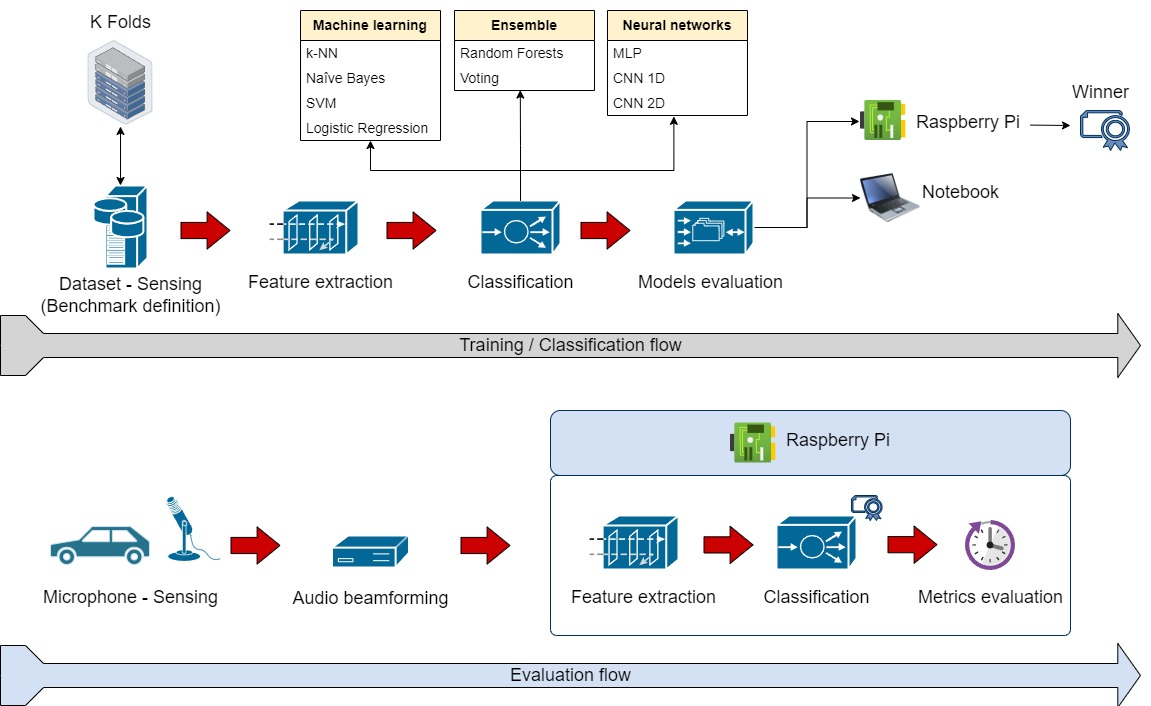
\includegraphics[width=.95\textwidth]{resources/images/050-methods/Methods_diagram.jpg}
        \smallcaption{Source: Author}
        \label{fig:methodology_illustration}
\end{figure}

The organization of this chapter is structured as follows: section \ref{sec:methods_HWSW} describes the software and hardware utilized in the experiments. In section \ref{sec:methods_dataset}, an overview of well-known datasets used in the systematic review is presented, along with a tailored proposal specifically for environmental sounds in the context of autonomous vehicles. Section \ref{sec:methods_normalization} introduces the concept of sample normalization within these datasets. The techniques for data augmentation are discussed in section \ref{sec:methods_augmentation}. Section \ref{sec:methods_feature_extraction} provides a comprehensive explanation of the methods employed for feature extraction. The \index{hyperparameter}hyperparameters used in the training process of the classifiers are outlined in section \ref{sec:methods_training_classifiers}, and finally, section \ref{sec:methods_evaluation} elucidates the evaluation procedures conducted on both the notebook and Raspberry Pi platform.


\section{HARDWARE AND SOFTWARE}
\label{sec:methods_HWSW}

The implementation of the algorithms in this study utilized the Anaconda software platform \cite{Anaconda86}, an open-source tool for library management that facilitates the creation of multiple virtual environments. Anaconda is particularly geared towards scientific computing and finds applications in various fields such as data science, machine learning, predictive analysis, and general scientific projects. The algorithms were written using Python version 3.9, either in PyCharm or in Jupyter notebooks, along with the \index{scikit-learn}scikit-learn library for machine learning techniques and ensemble methods \cite{scikitle61}, as well as the \index{Keras}Keras library for neural networks construction \cite{KerasDee32}. The Keras library is built on the \index{Tensorflow}Tensorflow framework \cite{TensorFl23}, serving as a high-level open-source \gls{api} for neural networks, and it is specifically designed to allow for fast implementation of both simple and highly complex neural networks, offering a modular, intuitive, and extensible interface. 

The training and testing of the models were performed on a notebook equipped with an Intel\textregistered{} Core\texttrademark{} i7-10850H CPU @2.70 \gls{g}\gls{hz}, 80 \gls{g}\gls{b} of RAM, and a Quadro T2000 graphics card with 4 \gls{g}\gls{b} of memory. The operational system in use was Windows 10 Enterprise.

Notably, the \gls{gpu} resources of the Quadro T2000 were instrumental in training the neural networks. However, it is worth mentioning that the \index{scikit-learn}scikit-learn library's algorithms lack support for GPU acceleration, resulting in a slower training process overall. On the other hand, the Tensorflow framework was designed specifically to leverage the extensive capabilities offered by \gls{gpu} resources, leading to training speeds approximately four times faster than when exclusively utilizing the CPU.


\section{DATASET}
\label{sec:methods_dataset}

The next subsections provide an overview of the prominent open-source datasets focusing on urban sound and \gls{esr}. These datasets are instrumental in this methodology for selecting suitable sound recognition systems for embedding purposes, while encompassing various categories that may not be exclusively urban-centric, they nonetheless encompass a sufficient repertoire of urban sounds that warrant their consideration for the purpose of this study, specially to establish a comparison baseline.

\subsection{ESC-10}
\label{subsec:dataset_ESC-10}

The compiled dataset in \textcite{PiczakESC2015} is divided into three sections: the primary labeled set encompasses 50 classes of diverse environmental sounds named ESC-50, a smaller proof-of-concept subset of 10 classes (ESC-10) was selected from the main dataset to serve as a simplified benchmark, and an additional dataset of unlabeled excerpts was included for unsupervised learning experiments (ESC-US). All datasets were constructed using sound clips sourced from publicly available recordings through the Freesound project \cite{Font_freesound2013}. The selection of classes for the labeled part of the dataset was done arbitrarily, with the aim of maintaining balance among major sound event types while considering limitations in the availability of diverse source recordings and subjectively evaluating the usefulness and distinctiveness of each class.

The ESC-10 dataset is a labeled set of 400 environmental recordings with 10 classes, 40 clips per class, 5-second-long recordings reconverted to a single channel (monophonic), sampling rate of 44,100 \gls{hz},  using Vorbis/Ogg compression @ 192 \gls{k}bit/\gls{s}, namely (Figure \ref{fig:methods_dataset_ESC-10}):

\begin{itemize}
    \item 001 - Dog bark;
    \item 002 - Rain;
    \item 003 - Sea waves;
    \item 004 - Baby cry;
    \item 005 - Clock tick;
    \item 006 - Person sneeze;
    \item 007 - Helicopter;
    \item 008 - Chainsaw;
    \item 009 - Rooster;
    \item 010 - Fire crackling.
\end{itemize}

\begin{figure}[htbp]
    \raggedright
        \caption{Wave form of randomly samples of each one of the classes within the dataset ESC-10.}
        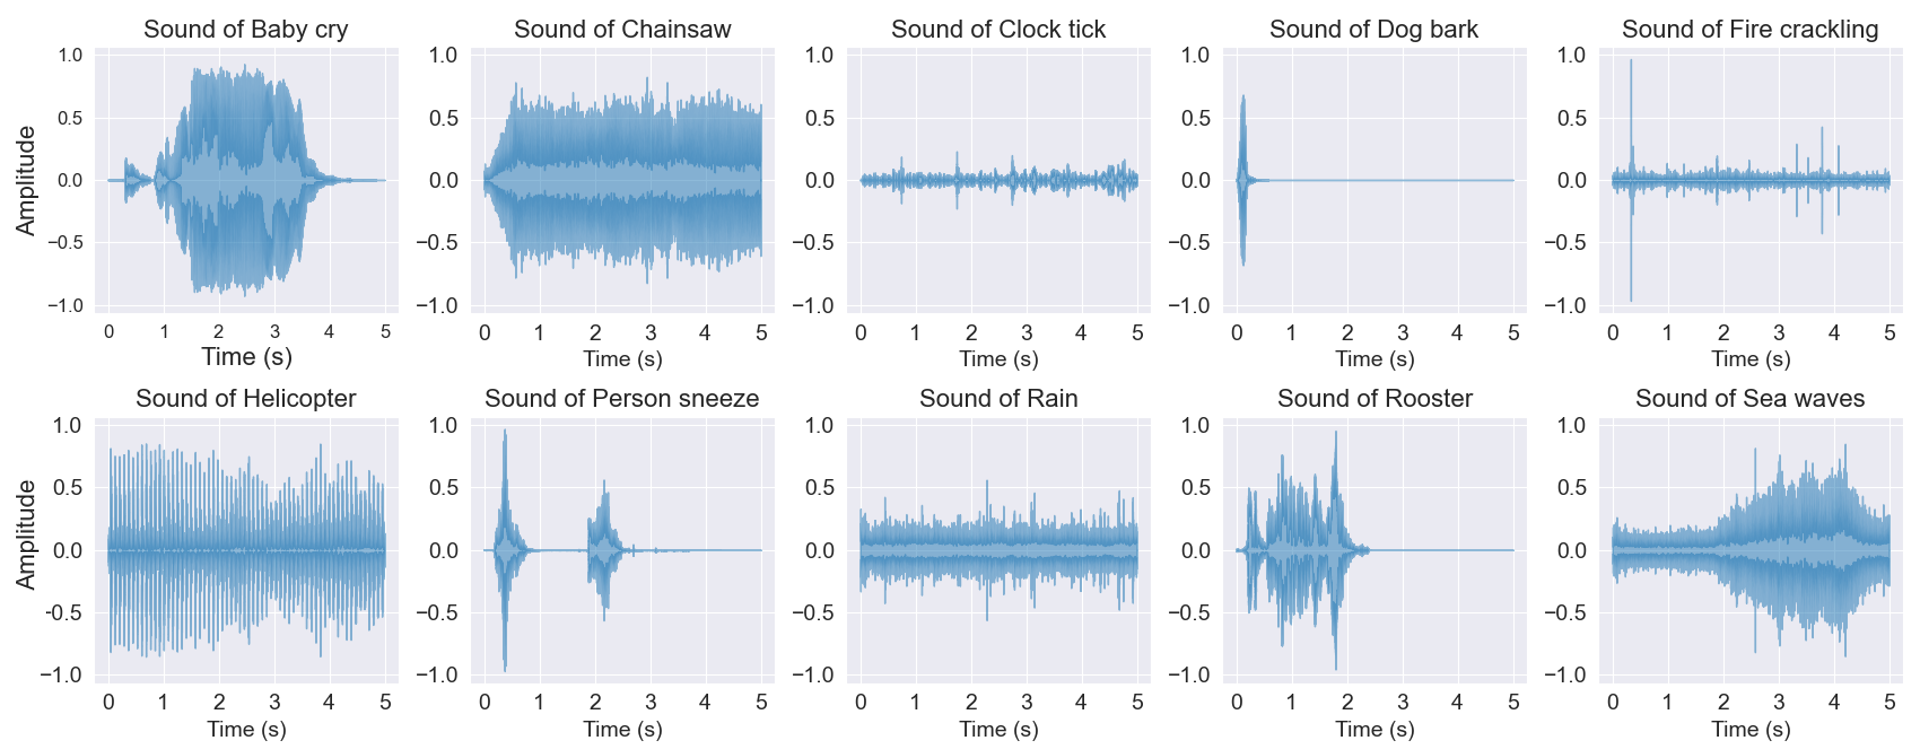
\includegraphics[width=1\textwidth]{resources/images/050-methods/Methods_dataset_ESC-10.png}
        \smallcaption{Source: Author}
        \label{fig:methods_dataset_ESC-10}
\end{figure}

The author propose the extraction of two distinct types of features, specifically, the \gls{zcr} and \gls{mfcc}, from each audio clip. The \gls{zcr} presents itself as a straightforward yet informative characteristic, while the application of \gls{mfcc} is widespread in the realm of speech processing and harmonic content analysis. The computation of \gls{mfcc}s was undertaken using the \index{Librosa}Librosa package \cite{McFee2015librosa_sw} with the default settings, giving rise to a frame length of 11.6 \gls{mi}\gls{s}. Following the exclusion of the 0\textsuperscript{th} coefficient, the initial 12 \gls{mfcc}s and the \gls{zcr} were aggregated for each clip via their respective mean and standard deviation across frames, resulting in a vector dimension of 26. These aggregated feature vectors were subsequently utilized as input for three distinct classifiers, namely, \gls{k-nn}, Random Forest ensemble, and \gls{svm} with a linear kernel. 

To assess the classifier performance, a 5-fold cross-validation regime was employed on the dataset ESC-10 during the learning phase, but unlikely other fold techniques, the author made it explicitly in his dataset metadata the fold split from 1 to 5. It was also confirmed in his code the for loop using these folds and therefore the same approach was carried out for the classifiers in this study.
For the \gls{k-nn}, the \index{hyperparameter}hyperparameter value for "k" was not specified in the article however, in the code was defined as 8. The Random Forest ensemble consisted of multiple decision trees, where each tree was trained on a randomly selected subset of features and samples from the dataset, but the number of trees in the ensemble was not mentioned. Again, analyzing the code made it possible to see the author's decision for 500 estimators. For \gls{svm} with a linear kernel, no specific hyperparameters were mentioned either, but in the code, the regularization parameter C was set to 0.5 \cite{PiczakESC2015}.

The results showed that for the ESC-10 dataset: 
\begin{itemize}
    \item \gls{k-nn} achieved an average classification accuracy ranging from 66.7\%;
    \item \gls{rf} ensemble achieved an average classification accuracy of 72.7\%;
    \item \gls{svm} had an average classification accuracy at 67\%. 
\end{itemize}

Considering the amount of classes involved in this study, the ECS-10 presents itself as better option to establish a baseline for the classifiers due its compact size and its original purpose as proof of concept.

\subsection{BDLib2}
\label{subsec:dataset_BDLib2}

The BDLib2 Environmental Sound Dataset created by \textcite{Bountourakis2015} was designed to compare existing machine learning techniques for recognizing environmental sounds and determine the most effective one, focusing on analyzing discrete sound events rather than general acoustic environments, with the long-term goal of applying this knowledge to soundscapes recognition.

The dataset was constructed by identifying and extracting 10-second-long audio clips that represent distinct sound categories originally sourced from the BBC Complete Sound Effects Library \cite{BBC2023} and Freesound project \cite{Font_freesound2013}. The authors took utmost care during the clip selection process to ensure the absence of background noise and prevent any overlap between the sound categories.

All recordings in the dataset are uncompressed single channel files in WAV format, captured at a sampling rate of 44,100 \gls{hz} and analyzed with a precision of 16 bits, summing 180 labeled files, structured into 10 classes, namely (Figure \ref{fig:methods_dataset_BDLib2}):
\begin{itemize}
    \item Airplanes;
    \item Alarms;
    \item Applause;
    \item Birds;
    \item Dogs; 
    \item Motorcycles;
    \item Rain;
    \item Rivers;
    \item Sea waves;
    \item Thunders. 
\end{itemize}

\begin{figure}[htbp]
    \raggedright
        \caption{Wave form of randomly samples of each one of the classes within the dataset BDLib2.}
        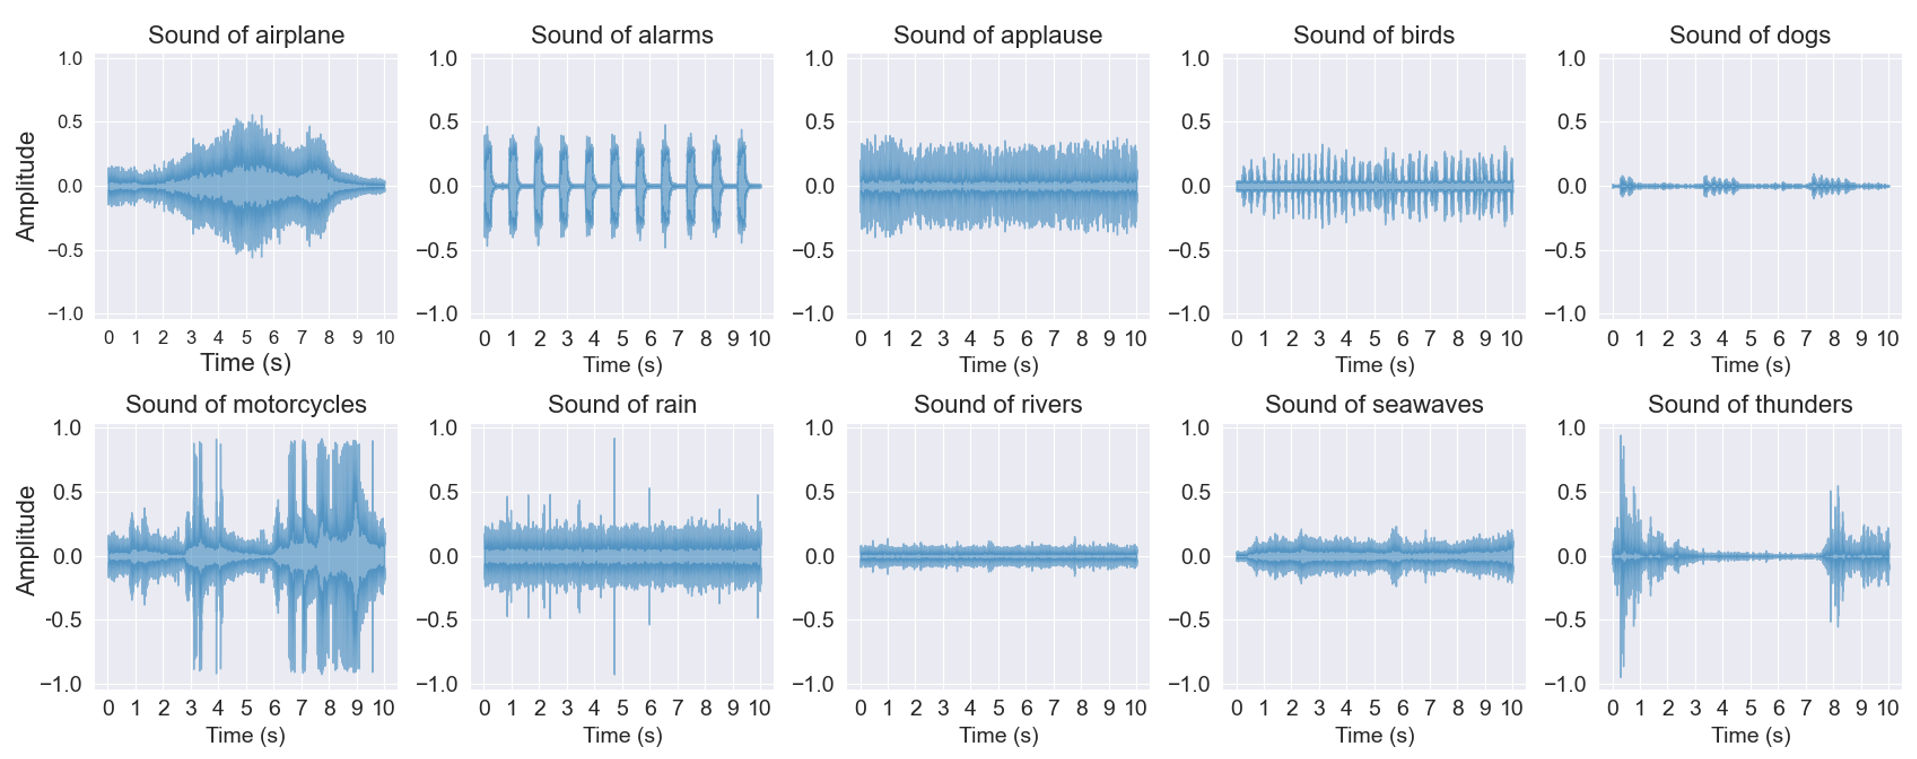
\includegraphics[width=1\textwidth]{resources/images/050-methods/Methods_dataset_BDLib2.png}
        \smallcaption{Source: Author}
        \label{fig:methods_dataset_BDLib2}
\end{figure}

While the original dataset experimental results \cite{Bountourakis2015} showed promising performance in classifying 7 different sound classes, it performed poorly in the recognition problem for 12 classes. Therefore, \textcite{Bountourakis2019} changed the library structure into new classes deliberately chosen to encompass a comprehensive range of sounds encountered in both indoor and outdoor soundscapes, aligning with established recognition schemes. To maintain diversity and authenticity, each class was uniformly represented in the database with 18 audio files, showcasing significant variations that reflect real-life scenarios.

Considering the total duration of the collected files amounts to 1,800 \gls{s}, which may be considered relatively small for the intended classification task, two commonly data augmentation techniques were applied to address the problem of limited data, namely time stretching with factors of 0.85 and 1.15, and pitch shifting by -4 and +4 semitones, carefully defined to ensure the semantic integrity of the transformed data. 

Following augmentation, the total duration of the complete database increased to 8,820 \gls{s}, which is comparable to the duration of similar reliable databases. It is worth noting that these augmentation techniques have been associated with improved model accuracy for environmental sound classification tasks \cite{Salamon2017} and are also presented in the systematic review of \textcite{Alli2022} for data augmentation and deep learning methods in sound classification.

In order to compare the frame-based method with temporal integration methods, several features showed in Table \ref{table:BDLib2_features_extracted} were extracted using two different window configurations: long windows for the frame-based method and short windows for the temporal integration methods. The short window had a duration of approximately 46 \gls{mi}\gls{s} with 50\% overlapping over 2,048 samples, while the long window had a duration of approximately 1.48 \gls{s} with 50\% overlapping over 65,536 samples. By extracting aggregated features over 64 subsequent short windows with 50\% overlapping, both methods achieved the same temporal resolution. For the sake of definition, 
texture window is commonly referred as an early integration technique when the process is carried out at the feature extraction level by consolidating short-time features across a larger frame \cite{Bountourakis2019}.

\begin{table}[ht!]
    \caption[Features extracted in the BDLib2 dataset]{Extracted audio features, including their respective dimensions (with a default dimension of 1 when not explicitly stated) and their acronym.}
    \label{table:BDLib2_features_extracted}
    \centering
    \begin{tabular}{
        >{\centering\arraybackslash}m{0.67\textwidth} | >{\centering\arraybackslash}m{0.27\textwidth}}
        \Xhline{2\arrayrulewidth}
        \rowcolor{lightgray}
        \textbf{Feature} & \textbf{Symbol} \\
        \hline
        Zero Crossing Rate & ZCR \\
        Root Mean Square & RMS \\
        Relative Difference Function & RDF  \\
        Spectral Centroid  & CEN \\
        Spectral Spread & SPR\\
        Spectral Flux & FLU \\
        Root Mean Square & RMS \\
        Spectral Roll-Off & ROL \\
        Spectral Skewness & SKEW \\
        Spectral Kurtosis & KURT \\
        Spectral Entropy & ENTR \\
        Spectral Variability & VAR \\
        Spectral Smoothness & SMO \\
        Spectral Flatness Measure (24) & SFM \\
        Spectral Crest Factor (24) & CSF \\
        Brightness  & BRI \\
        Roughness & ROU \\
        Irregularity & IRR \\
        \gls{mfcc} (13) & \gls{mfcc} \\
        Delta \gls{mfcc} (13) & DMFCC \\
        \gls{lpcc} (12) & \gls{lpcc} \\
        \Xhline{2\arrayrulewidth}
    \end{tabular}
    \smallcaption{Source: \textcite{Bountourakis2019}, page 413}
\end{table}

 Beside the mean, \gls{std}, skewness, and kurtosis used in most temporal integration methods, 4 additional metrics were proposed:

 \begin{itemize}
    \item \gls{msd}: This metric quantifies the amount of variation and frequency of changes in successive feature values within a texture window;
    \item \gls{mcr}: Inspired by \gls{zcr}, MCR estimates the alternations of successive feature values with respect to their mean value within a texture window;
    \item \gls{fla}: Similar to Spectral Flatness, this metric calculates temporal flatness by dividing the geometric mean of feature values by their arithmetic mean within a texture window;
    \item \gls{crf}:  \gls{crf} is calculated by dividing the maximum value by the mean value of feature values within a texture window, similar to how it is used for wave-forms.
\end{itemize}
	
To determine the most effective machine learning technique for the aforementioned dataset, 3 different methods for feature aggregation were proposed to generate feature vectors for sound classification, namely:

\begin{itemize}
    \item \gls{sfb}: a vector with dimension of 100 considering all features extracted in the Table \ref{table:BDLib2_features_extracted}, discarding the \gls{mfcc}-0 that is fundamentally related to the signal's energy;
    \item \gls{sti}: a vector with dimension of 96 build through the mean, standard deviation, skewness, and kurtosis of the following 12 baseline features: \gls{mfcc}s, CEN, SPR, SKEW, KURT, ROL, ENTR, BRI, VAR, RMS, ZCR, and RDF;
    \item \gls{eti}: identical to \gls{sti}, but including the 4 additional metrics previously described (MSD, MCR, FLA and CRF), adding 96 dimensions to the vector leading to a final dimension of 192.
\end{itemize}

Feature ranking algorithms were employed to select the most relevant features for each method, followed by the utilization of \gls{lr}, \gls{ann}, and \gls{glm} classifiers for classification purposes. There were no mention of hyperparameters for \gls{lr} and \gls{glm}, on the other hand, the \gls{ann} architecture consisted of 2 hidden layers, with the number of neurons in each hidden layer being equivalent to half the sum of the input and output dimensions, and a dropout layer was then incorporated. The remaining parameters followed a conventional configuration: the \gls{relu} activation function was utilized for the intermediate layers, SoftMax function for the output layer, Categorical Cross-Entropy employed as the loss function, and Adam utilized as the optimizer. The learning rate was set at 0.01 with a dropout rate of 25\%.

The training process involved splitting the sound files into a training set with 12 files per class and a testing set with 6 files per class, ensuring that the algorithms were tested on unseen data. To prevent overfitting and ensure unbiased results, a 3-fold cross-validation regime was employed during the learning phase and although a metadata was not available, the same principle used in the ESC-10 dataset was used since there are 3 distinct folds available after unzipping the downloaded files. The \gls{eti} method demonstrated higher accuracy than the \gls{sti} method, and among the classifiers, \gls{ann} performed the best with 81.5\% accuracy, followed by \gls{glm} with 80.4\% and \gls{lr} with 74.8\%. Nevertheless, in light of the objective of conducting comparisons with the other datasets in this study, it is more appropriate to utilize the findings from the \gls{sti}:

\begin{itemize}
    \item \gls{ann} achieved an average classification accuracy of  75.2\%;
    \item \gls{glm} following, with an average classification accuracy of 75.0\%;
    \item \gls{lr} by last, with an average classification accuracy at 73.6\%. 
\end{itemize}


\subsection{UrbanSound8K}
\label{subsec:dataset_US8K}

The authors of this dataset developed a taxonomy based on a subset of a previous taxonomy specific to urban acoustic environments, focusing on low-level sound sources like "car horn" and "jackhammer" instead of broader categories. They also analyzed noise complaints filed through New York City's 311 service to identify frequently complained about sound categories relevant to urban sound research \cite{Salamon2014}.

The UrbanSound dataset was created by downloading field recordings from the Freesound repository \cite{Font_freesound2013} and meticulously verifying each recording to ensure the presence of the sound of interest. After the filtering process, 1,302 recordings totaling over 27 hours of audio were obtained. In the next step, the recordings were labeled at the start and end times of every occurrence of a sound, and a salience description to indicate foreground or background perception was added. This resulted in 3,075 labeled occurrences amounting to 18.5 hours of labeled audio. Finally, for sound source identification research, an additional subset called \gls{us8k} was created, encompassing short audio snippets segmented into 4 \gls{s} slices using a sliding window approach with a 2 \gls{s} overlap, totaling 8,732 labeled files.

Using the open-source audio editing software \index{Audacity}Audacity \cite{Audacity2024}, it was possible to identify that all recordings in the dataset are uncompressed multi channel files (stereo) in WAV format, captured at a sampling rate between 8,000 and 192,000 \gls{hz} and analyzed with a precision of 32 bits, pre-arranged into ten folds (labeled fold1 to fold10) to facilitate the replication and comparison of the automatically generated classification results, namely (Figure \ref{fig:methods_dataset_US8K}):
\begin{itemize}
    \item air\_conditioner;
    \item car\_horn;
    \item children\_playing; 
    \item dog\_bark; 
    \item drilling; 
    \item enginge\_idling; 
    \item gun\_shot; 
    \item jackhammer; 
    \item siren; 
    \item street\_music.
\end{itemize}

\vspace{12pt}

\begin{figure}[htbp]
    \raggedright
        \caption{Wave form of randomly samples of each one of the classes within the dataset \gls{us8k}.}
        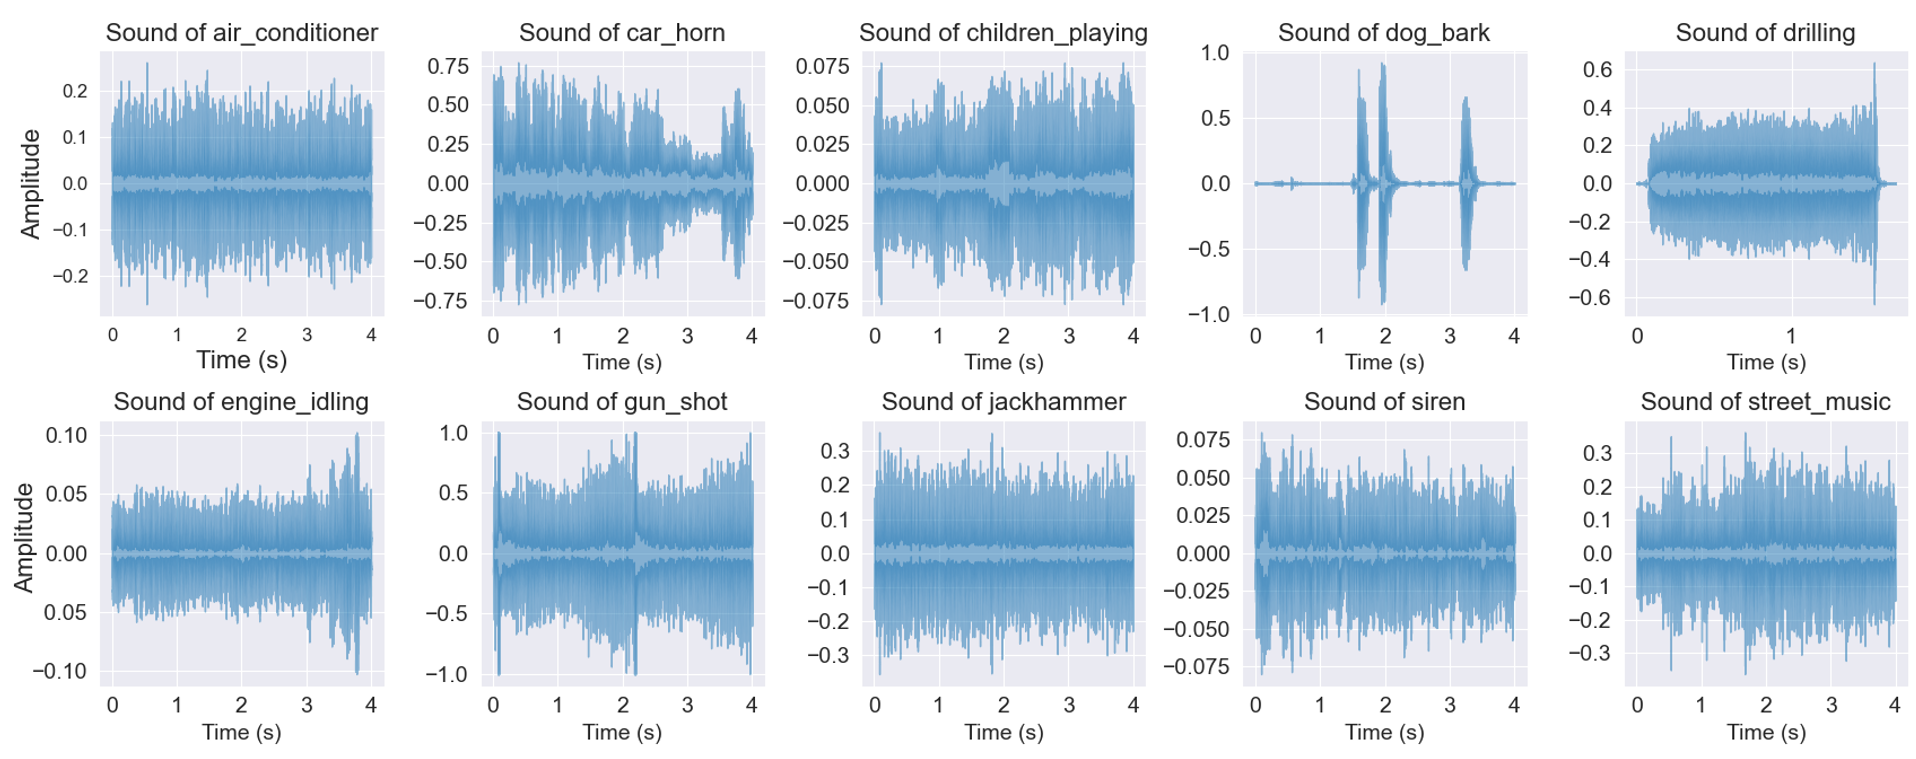
\includegraphics[width=1\textwidth]{resources/images/050-methods/Methods_dataset_US8K.png}
        \smallcaption{Source: Author}
        \label{fig:methods_dataset_US8K}
\end{figure}

The sound classification process was performed in the \gls{us8k} aiming to learn about the characteristics of the dataset rather than an optimal combination of feature/classifier parameters. Considering the reasonable amount of recording hours in the dataset, the authors extracted \gls{mfcc} from the audio clips with no previous augmentation technique implemented. The features were extracted on a per-frame basis with a window size of 23.2 \gls{mi}\gls{s} and 50\% frame overlap using the first 25 \gls{mfcc} coefficients from the initially 40 Mel bands computed. Summary statistics such as minimum, maximum, median, mean, variance, skewness, kurtosis along with mean and variance of first and second derivative coefficients were computed to create a feature vector of dimensionality equal to 225 per audio clip.

In order to experiment with different classification algorithms and different audio clip lengths, a 10-fold cross-validation was utilized through a random allocation process to ensure that clips from the same original recording were not used for both training and testing, thus avoiding artificially high classification accuracy results. The machine learning classifier considered were: Decision Tree, \gls{k-nn} with "k" set to 5 neighbors, \gls{rf} with 500 trees, \gls{svm} with a \gls{rbf} kernel, and a majority vote classifier named ZeroR. The authors analyzed the classifiers performance considering a window of 1 \gls{s} to 10 \gls{s} for the audio clips, and most notably, it was noticed a uniform pattern in behavior across all classifiers, with performance maintaining stability from 10 \gls{s} to 6 \gls{s}, followed by a gradual decline. Yet, when focusing on the top-performing classifiers (\gls{svm} and \gls{rf}), there was no statistically significant distinction in performance between 6 \gls{s} clips and 4 \gls{s} clips, although the difference becomes significant when considering clips below 4 \gls{s}. As the dataset was published with a 4 \gls{s} window, the following results for each classifier were estimated below (values were not explicit, rather shown by a chart):

\begin{itemize}
    \item \gls{svm} was on top with an estimated classification accuracy of 69.0\%;
    \item \gls{rf} following, with an estimated classification accuracy of 66.0\%;
    \item \gls{k-nn} achieved estimated classification accuracy of 56.0\%;
    \item Decision Tree achieved estimated classification accuracy of 48.0\%;
    \item Voting classifier by last, with an estimated classification accuracy of 10.0\%. 
\end{itemize}


\subsection{Tailored dataset (US8K\_AV)}
\label{subsec:dataset_US8K_AV}

The available datasets may not encompass the specific categories relevant to the context outlined in this study, and generating new datasets is a labor-intensive and time-consuming endeavor. To overcome this situation,  the evaluation of the existing dataset was carried out subjectively, taking into account the relevance of classes that could potentially be integrated into the C-Bot during the third phase (Figure \ref{fig:methods_dataset_US8K_AV}). A new dataset, denoted as US8K\_AV, which stands for UrbanSound8K for Autonomous Vehicles, was constructed under specific conditions to optimize performance: irrelevant classes were eliminated, less relevant urban sounds were consolidated into new classes, and contextually relevant classes were preserved \cite{florentino2024}.

To maintain the same class distribution as the original dataset, the new class "background" was populated with 1,000 randomly selected samples from the original classes. Further on, the class "silence" was also added, sourced from the Freesound project \cite{Font_freesound2013} to complement the dataset, aiming to enhance the utility and accuracy of the inferences during live predictions. Special attention was given to preserve the dataset specification regarding the k-fold distribution, thus avoiding class contamination with sound segments from the same sound source. Upon completing this process, the US8K\_AV dataset comprised 4,908 files, distributed among 6 classes preserving the 10-fold split for cross-validation, with a total duration of 4.94 hours of recorded sounds and 3.27 GB of total size. A detailed description of each of these classes is provided below and the dataset statistics in table \ref{table:US8K_AV_statistics}:

\begin{itemize}
    \item \textbf{"dog\_bark"}: characterized by a sharp and abrupt sound, produced by canines, often indicating territorial defense or alertness to intrusions. Contains high variation in pitch and frequency along time. 0.87 h within 1,000 audio samples;
    \item \textbf{"children\_playing"}: this class encompasses a range of sounds such as laughter, shouting, and running, typically generated by groups of children engaged in recreational activities in outdoor or indoor environments. 1.10 h within 1,000 audio samples;
    \item \textbf{"siren"}: mainly loud, high pitch, oscillating tone used primarily by emergency vehicles such as ambulances, fire trucks, and police cars to signal their presence and urgency in traffic. 1.01 h within 929 audio samples;
    \item \textbf{"car\_horn"}: produced by motor vehicles, car horns generate a short, high-decibel honk intended to alert other drivers and pedestrians to potential hazards or to communicate driver intentions. 0.29 h within 429 audio samples;
    \item \textbf{"background"}: comprising a mixture of drilling, engine idling, jackhammer operations, and street music, this class represents ambient urban noise often encountered in metropolitan areas. The diverse soundscape serves as a backdrop that may mask or interfere with the detection of other distinct auditory events. 1.05 h within 1,000 audio samples;
    \item \textbf{"silence"}: characterized by a near-absence of discernible sound waves, this class represents periods of minimal or no auditory activity. Silence is essential for calibrating baseline noise levels and for distinguishing between meaningful audio events and background noise. 0.61 h within 550 audio samples.
\end{itemize}


\begin{figure}[htbp]
    \raggedright
        \caption{Subjective evaluation of the classes within the datasets ESC-10, BDLib2 and \gls{us8k} related to autonomous vehicles and proposal for a tailored dataset based on the \gls{us8k} classes.}
        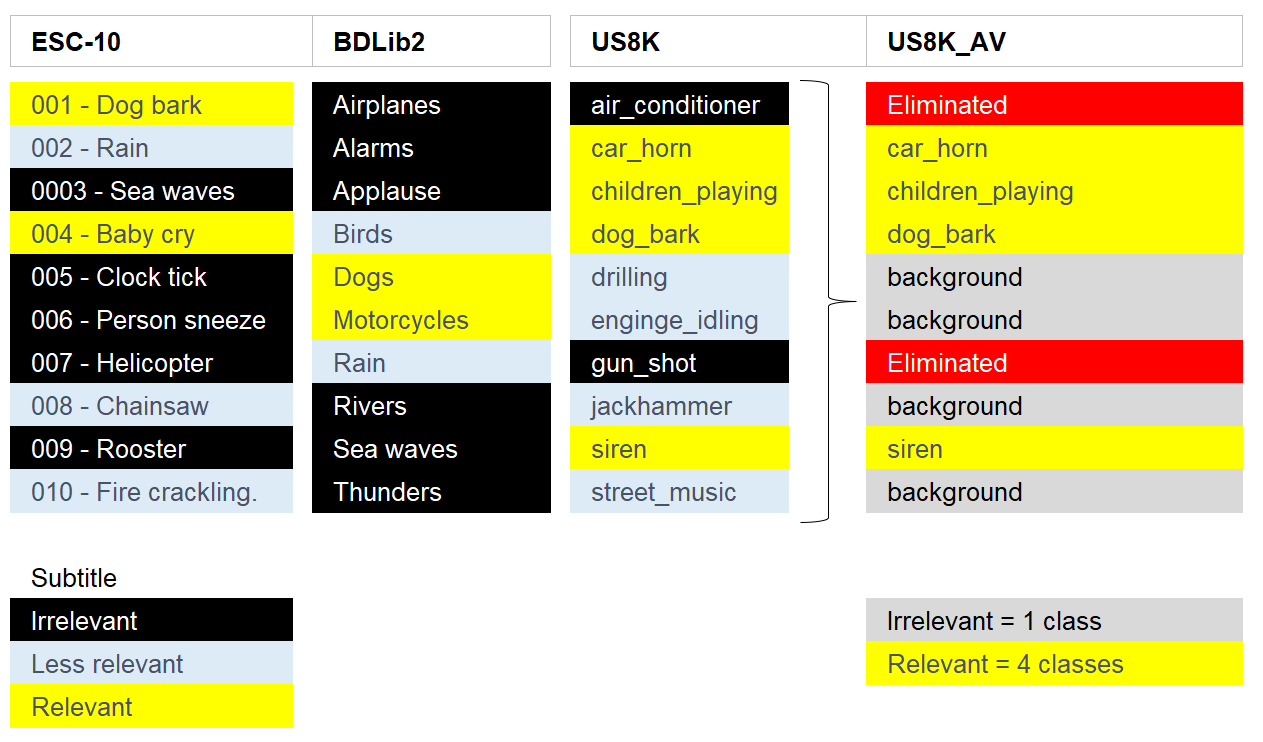
\includegraphics[width=1\textwidth]{resources/images/050-methods/Methods_dataset_US8K_AV.png}
        \smallcaption{Source: Author}
        \label{fig:methods_dataset_US8K_AV}
\end{figure}

\begin{table}[ht!]
    \caption[Statistics on the tailored dataset US8K\_AV]{Total size, number of files, unique sampling rates and, average duration corresponding to each class of the US8K\_AV dataset.}
    \label{table:US8K_AV_statistics}
    \centering
    \begin{tabular}{
        >{\arraybackslash}m{0.05\textwidth} | >
        {\raggedright\arraybackslash}m{0.15\textwidth} | >
        {\raggedright\arraybackslash}m{0.10\textwidth} | >
        {\raggedright\arraybackslash}m{0.11\textwidth} | >
        {\raggedright\arraybackslash}m{0.28\textwidth} | >
        {\raggedright\arraybackslash}m{0.13\textwidth}}
        \Xhline{2\arrayrulewidth}
        \rowcolor{lightgray}
        Fold & Folder name & Nr. files & Size & Min, Max sampling rates & Av. sample \\ 
        \rowcolor{lightgray}
        &  &  & (MB) & (hz) & duration (s) \\        
        \hline
        1 & fold1 & 478 & 350.26 & 8,000 to 96,000 & 3.59 \\
        2 & fold2 & 485 & 334.86 & 11,025 to 96,000 & 3.58 \\
        3 & fold3 & 536 & 332.36 & 11,025 to 96,000 & 3.68 \\
        4 & fold4 & 599 & 422.08 & 11,025 to 96,000 & 3.63 \\
        5 & fold5 & 529 & 334.56 & 16,000 to 96,000 & 3.62 \\
        6 & fold6 & 460 & 276.28 & 11,025 to 96,000 & 3.62 \\
        7 & fold7 & 465 & 299.23 & 11,025 to 96,000 & 3.69 \\
        8 & fold8 & 441 & 279.12 & 8,000 to 192,000 & 3.58 \\
        9 & fold9 & 447 & 312.98 & 11,025 to 96,000 & 3.61 \\
        10 & fold10 & 468 & 328.68 & 11,025 to 96,000 & 3.62 \\
        \hline
    \end{tabular}
    \smallcaption{Source: Author}
\end{table}


\section{NORMALIZATION}
\label{sec:methods_normalization}

The concept of audio normalization entails the process of standardizing audio signals by harmonizing their amplitudes to a unified scale. Typically, this is achieved by manipulating the gain or volume of the audio while preserving its relative dynamics in order to establish a consistent level across all audio recordings, thereby minimizing the influence of factors such as disparate recording devices, microphone sensitivities, and environmental circumstances, bringing as consequences a consistency across different datasets, robustness to recording conditions and improved generalization \cite{Mueller2016}.

There are multiple audio normalization techniques, and the following compilation outlines the most pertinent approaches according to \textcite{Mueller2021}:

 \begin{itemize}
    \item Peak amplitude normalization: it involves adjusting the amplitude so that the highest point in the audio signal reaches a specified target level, ensuring that no part of the signal is clipped;
    \item \gls{rms} normalization: this method takes into account the overall energy distribution averaging its power signal and is less sensitive to short-term amplitude fluctuations;
    \item Perceptual loudness normalization: essentially identical do the \gls{rms} normalization but based on perceived loudness which considers human auditory perception.
    \item Frame-level normalization: in involves clipping the audio recording at a smaller time scale, such as individual frames or segments to address variations within the audio signal over time, thus capturing dynamic patterns more effectively;
    \item Duration adjustment: while not strictly a normalization technique, adjusting the duration of audio segments to a common length is often performed in conjunction with amplitude normalization to ensures that the classifiers receive input of consistent duration in the training process.
\end{itemize}

Fundamentally, the authors of the aforementioned datasets stated they were already normalized to reach an amplitude peak of 80 \gls{db}, nonetheless, such statement was also confirmed during the data exploration in the Jupyter notebooks. \gls{rms} and perceptual loudness normalization were not explicitly mentioned in the related work, and though conceptually relevant, they were not utilized in this study.

During the preliminary classifiers experiments, the concept of frame-level normalization was investigated following the procedures of \textcite{Silva2019} and \textcite{Lhoest2021}. This involved dividing the audio signal into $n$ short audio clips, each lasting ~1 \gls{s} and overlapping with a 50\% margin (comprising 44 frames at a sampling rate of 22,050 \gls{hz} and a hop length of 512). These shorter audio clips were only temporarily stored in an array, until the relevant features were extracted from them. This technique was not considered in this study as an augmentation technique \textit{per se}, rather was used in the section \ref{sec:methods_feature_extraction} as supporting tool for one of the feature extraction methods.

Several classes in the datasets, particularly ESC-10, ESC-50, and BDLib2, contain audio files where the original sound constitutes only 30\% to 50\% of the total duration, with the remaining portion being silence, as illustrated in Figure \ref{fig:methods_normalization_original_wave_form} using a random sample.

\begin{figure}[htbp]
    \raggedright
        \caption{Wave form of an audio sample from the dataset ESC-10, class "001 - Dog bark", file name: 3-170015-A.ogg, illustrating most of the audio duration as silence or near-silence.}
        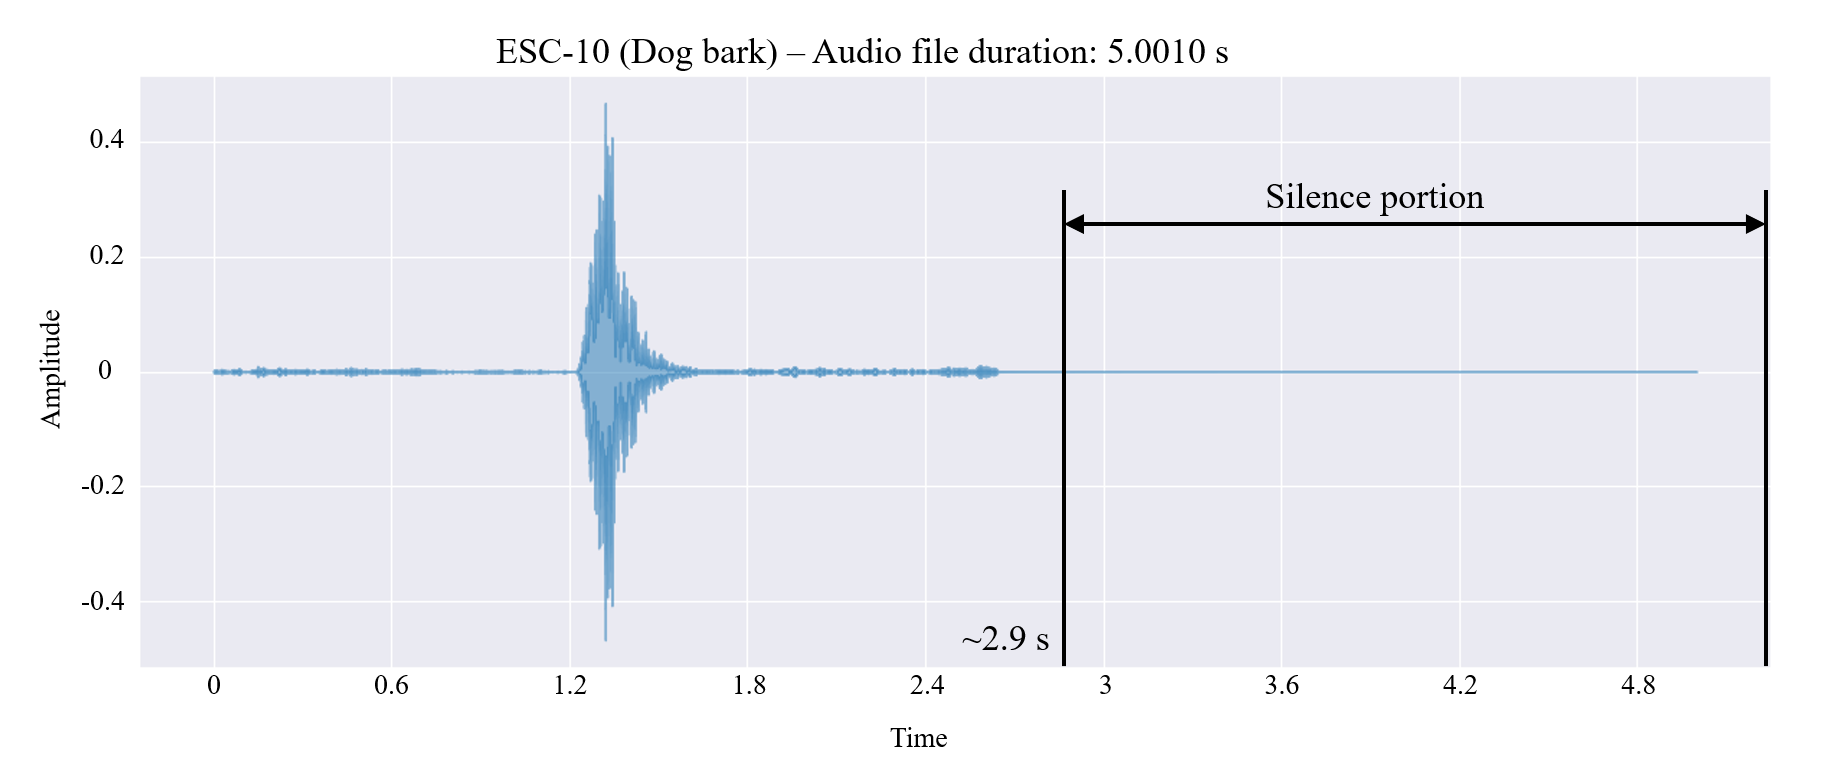
\includegraphics[width=1\textwidth]{resources/images/050-methods/Methods_normalization_original.png}
        \smallcaption{Source: Author}
        \label{fig:methods_normalization_original_wave_form}
\end{figure}

This type of audio data significantly reduces the accuracy of the classifiers, and therefore, the technique of duration adjustment was merged with trimming and implemented in this study. According to \textcite{Mushtaq2020b}, when applying the trim silence technique as a pre-processing method to the entire audio dataset, a common challenge arises in determining the precise threshold value in \gls{db} \underline{below the reference point} (80 \gls{db} confirmed by peak amplitude normalization), which indicates silence. The improper selection of this threshold value has the potential to lead to the loss of crucial information contained within the audio data and although stated in the article that the threshold of 40 \gls{db} has been settled as the most effective silence trimming value for the used datasets, this value was not suitable when merged with the duration adjustment technique as shown in Figure \ref{fig:methods_normalization_40_db_x_60_db_wave_form} where approximately 1.1 \gls{s} of the audio data was lost when compared with the threshold of this study.

\begin{figure}[htbp]
    \raggedright
        \caption{Wave form of the audio file 3-170015-A.ogg trimmed to 40 \gls{db} and 60 \gls{db} resulting in approximately 1.1 \gls{s} of data loss.}
        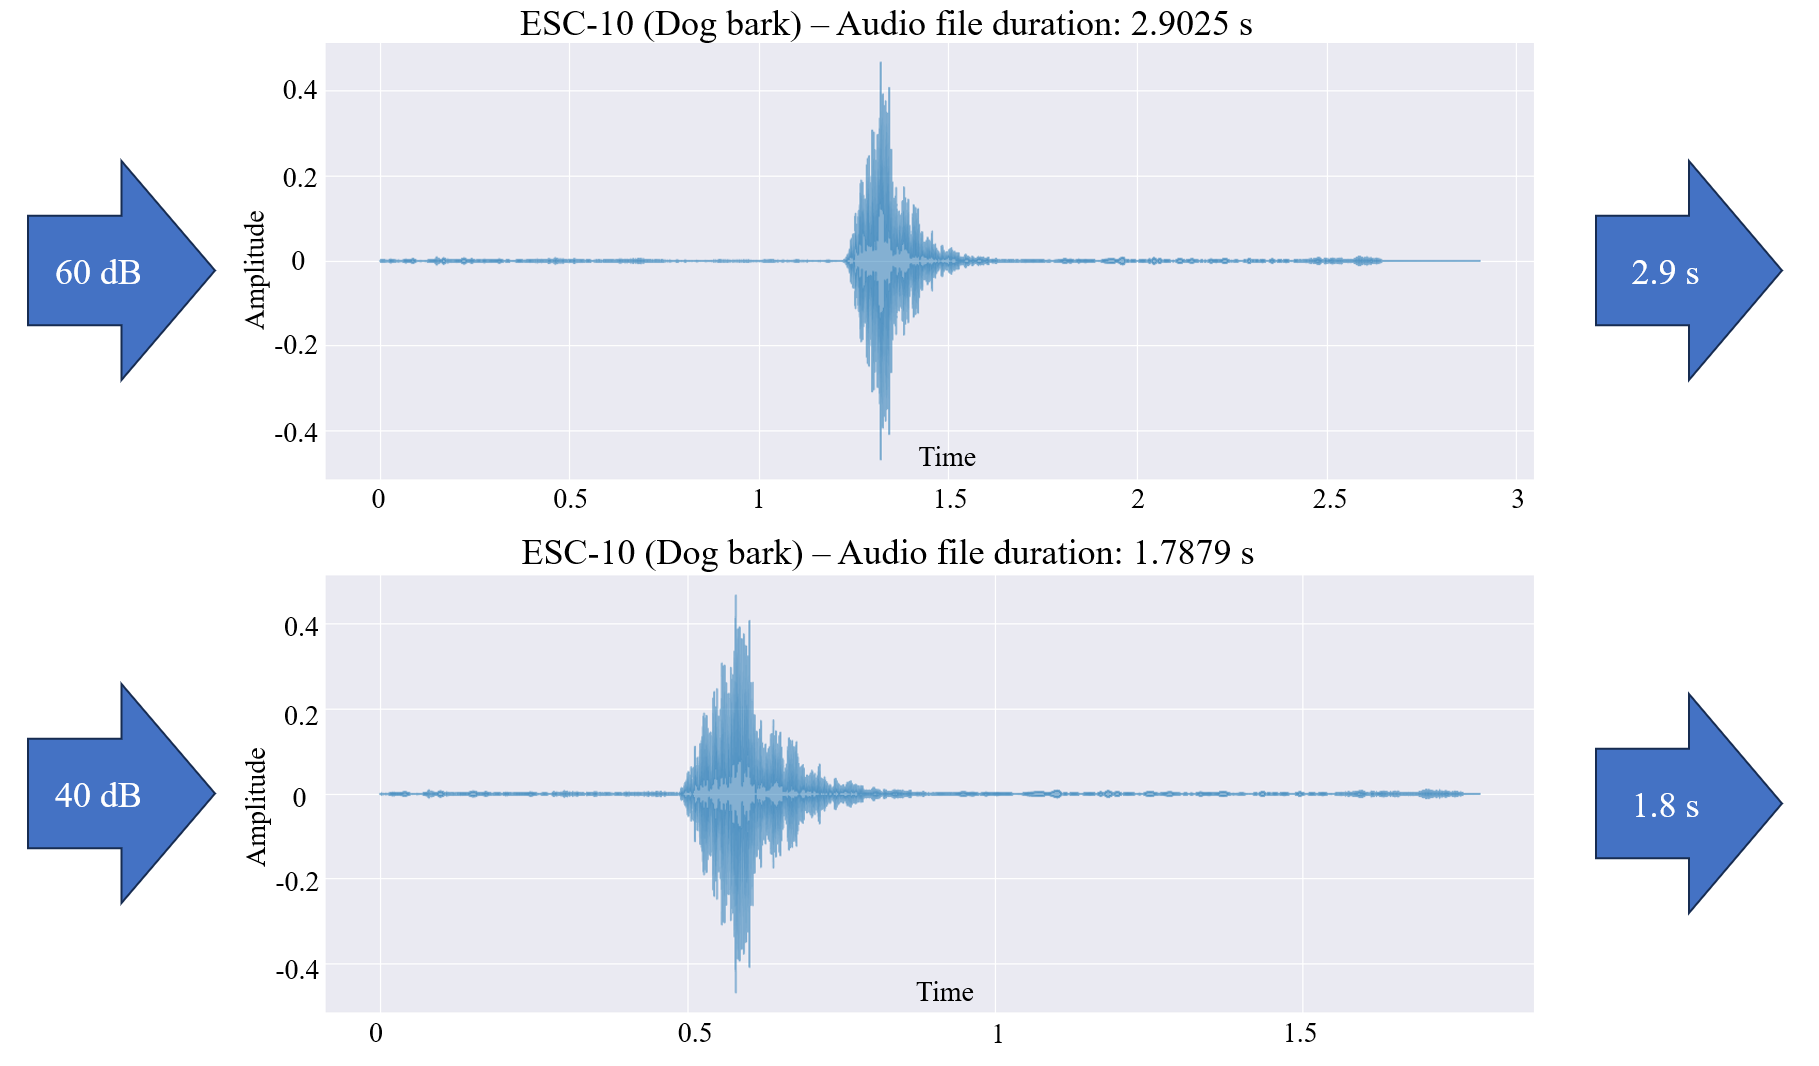
\includegraphics[width=1\textwidth]{resources/images/050-methods/Methods_normalization_comparison_40db_60db.png}
        \smallcaption{Source: Author}
        \label{fig:methods_normalization_40_db_x_60_db_wave_form}
\end{figure}


\begin{figure}[htbp]
    \raggedright
        \caption{Wave form of the audio file 3-170015-A.ogg trimmed to 60 \gls{db} and concatenated to reach the target duration of 5 \gls{s}.}
        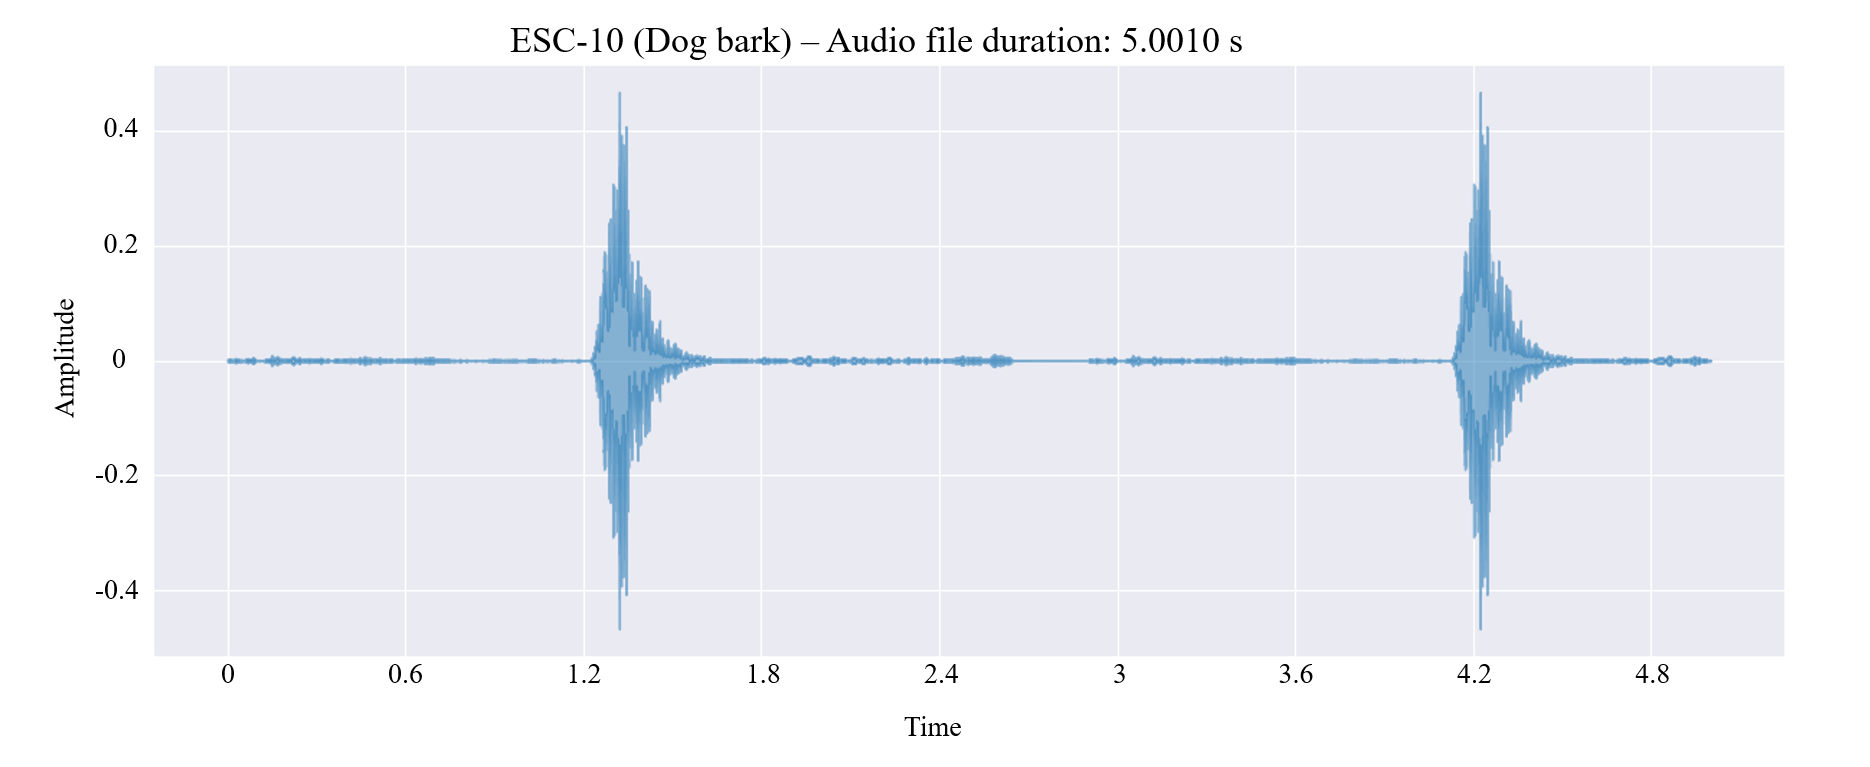
\includegraphics[width=1\textwidth]{resources/images/050-methods/Methods_normalization_normalized.png}
        \smallcaption{Source: Author}
        \label{fig:methods_normalization_normalized_audio_data}
\end{figure}

The value of 60 \gls{db} was settled as threshold after several investigations using the split function of the package \index{Librosa}Librosa \cite{McFee2015librosa_sw}, which took an audio signal as input and returned a NumPy array of intervals, where each interval is represented as a tuple of start and end times (in samples) of non-silent audio. The for loop continues, concatenating the non-silent audio frames until the target duration is exactly achieved for each dataset (ESC-10: 5 \gls{s}, BDLib2: 10 \gls{s} and UrbanSound8K: 4 \gls{s}). The final audio wave form of the normalized audio data is shown in the Figure \ref{fig:methods_normalization_normalized_audio_data}. Significantly, the normalization process primarily focused on the duration adjustment rather than trimming in the datasets, as trimming was observed to occur infrequently (after the process, approximately 20\% of the audio data exhibited some form of trimming).


\section{AUGMENTATION}
\label{sec:methods_augmentation}

In general, augmentation techniques can help overcome the problem of limited labeled data, which is quite common in many application domains, and audio recognition is no exception. By artificially introducing variations in the audio data during training, audio augmentation expands the dataset and allows the models to learn more robust and discriminative features, thus improving their generalization capabilities, resulting in better equipped models to handle real-world scenarios where the sounds may exhibit variations in pitch, duration, and amplitude. Additionally, audio augmentation helps the models become less sensitive to background noise by training them on a wider range of acoustic conditions.

In the systematic review for deep learning methods and data augmentation in sound classification, \textcite{Alli2022} ranked the technique of noise addition with the largest number of occurrences, accounting for 22 publications (39.2\%). The subsequent highest number of occurrences was attributed to the time shift method, encompassing 15 publications (26.7\%), following closely behind were the \gls{gan} based models and pitch shifting, each accounting for 12 publications (21.4\%). Additionally, alternative methods, namely time stretching, mix-up, and background noise, summed 10 (17.8\%), 9 (16.1\%), and 8 (13.6\%) publications, respectively. 

 Time stretching, pitch shifting, dynamic range compression and background noise were also used by \textcite{Salamon2017} in their deep convolutional neural network classifier. \textcite{Mushtaq2020b} utilized time stretching, pitch shifting, white noise addition and silence trimming (that dwells between normalization and augmentation techniques) in their regularized deep convolutional neural network while \textcite{Bountourakis2019} considered only time stretching and pitch shifting. Techniques commonly used in the speech recognition helm such as warping the features, masking blocks of frequency channels, and masking blocks of time steps \cite{Park2019} were not found explicitly in the related work and therefore were not considered in this study.

After experimenting the data augmentation within all the datasets, five techniques were selected and implemented in this study, namely \textbf{time stretches quickly} where the time of each audio clip of the dataset was stretched by a factor of 1.15 and \textbf{time stretch slowly}, acting in the opposite direction, the audio clip was slowed down by a factor of 0.85 (Figure \ref{fig:methods_augmentation_time_stretch}).

\begin{figure}[htbp]
    \raggedright
        \caption{Wave form of the audio file 3-170015-A.ogg augmented using the time stretch technique with factor 0.85 and 1.15.}
        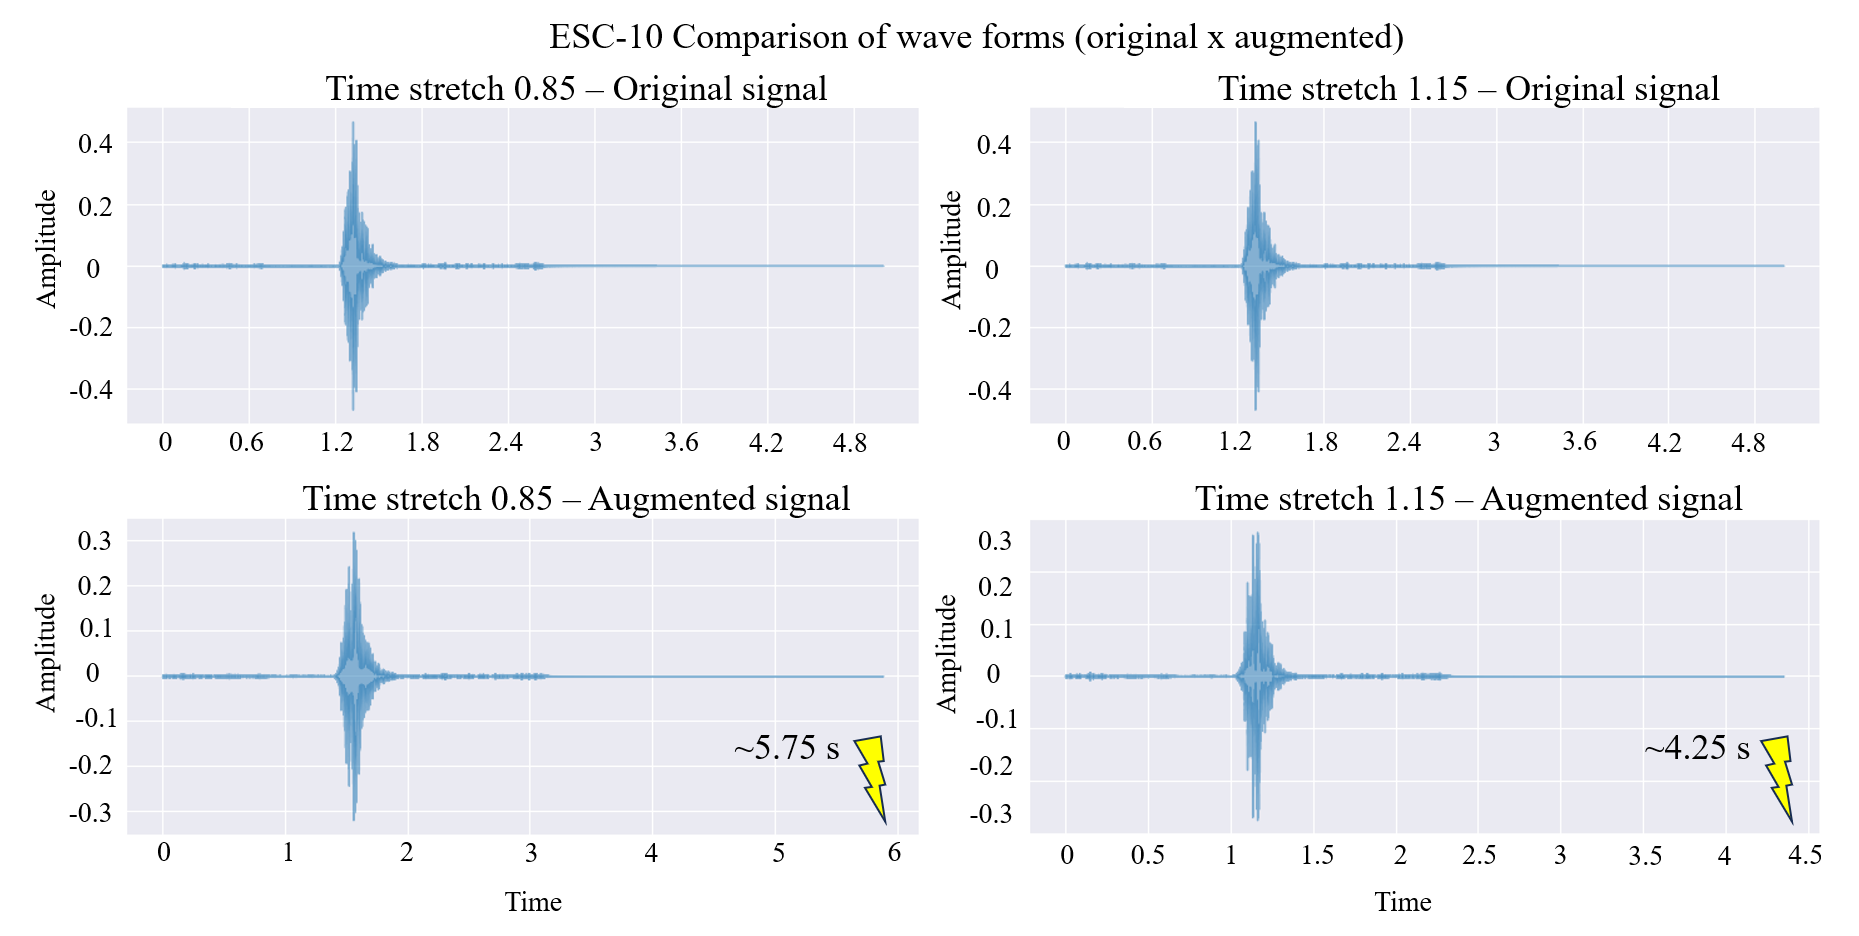
\includegraphics[width=.98\textwidth]{resources/images/050-methods/Methods_augmentation_time_stretching.png}
        \smallcaption{Source: Author}
        \label{fig:methods_augmentation_time_stretch}
\end{figure}

\textbf{Pitch shifting positively} that increased the pitch of the audio clip in 4 semitones, and again, inversely, \textbf{pitch shifting negatively} that decreased the pitch of the audio clip in 4 semitones, keeping the total duration of the audio file the same as shown in the spectrograms of Figure \ref{fig:methods_augmentation_pitch_shifting}. 

\begin{figure}[htbp]
    \raggedright
        \caption{Mel frequency spectrogram of the audio file 3-170015-A.ogg augmented using the pitch shifting technique with +4 and -4 semitones.}
        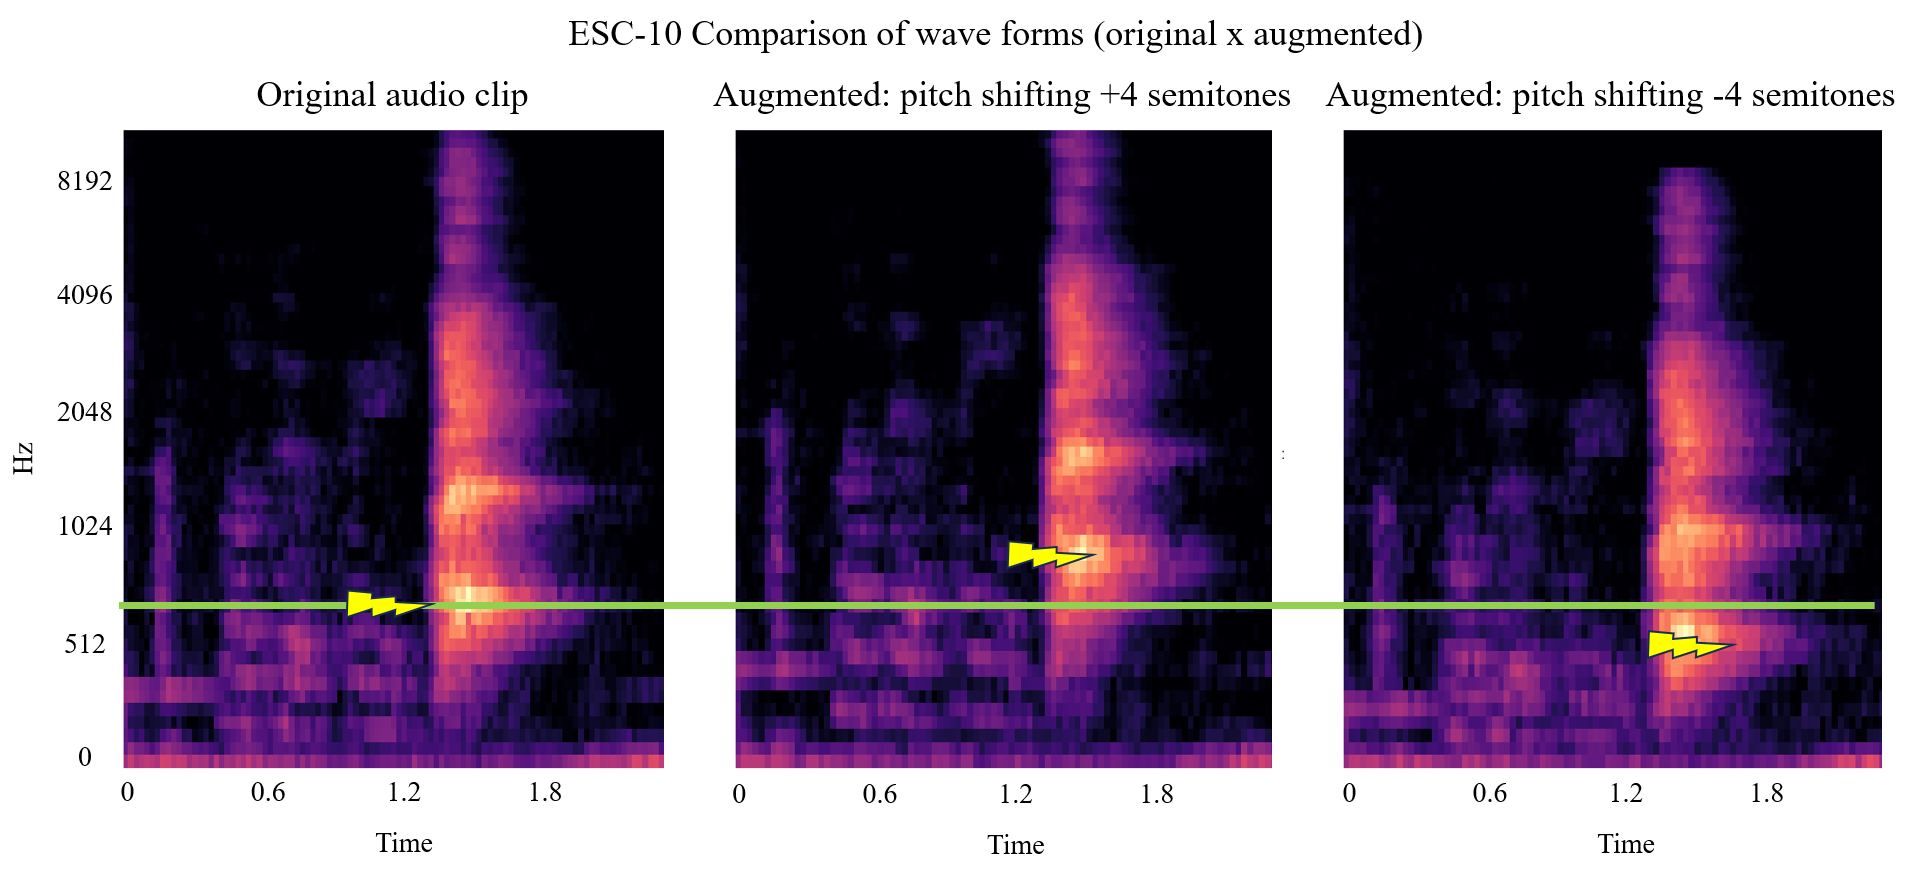
\includegraphics[width=.98\textwidth]{resources/images/050-methods/Methods_augmentation_pitch_shifting.png}
        \smallcaption{Source: Author}
        \label{fig:methods_augmentation_pitch_shifting}
\end{figure}

And finally, \textbf{time shifting randomly}, where the algorithm initialize a random integer (start\_) within the range [-4,800, 4,800] using Numpy random.uniform. Depending on the value of start\_, a time shift is applied to the audio clip. If start\_ is negative, the audio is shifted to the right by start\_ samples, and random noise is added at the beginning. If start\_ is positive, the audio is shifted to the left by -start\_ samples, and random noise is added at the end (Figure \ref{fig:methods_augmentation_time_shifting}).

\begin{figure}[htbp]
    \raggedright
        \caption{Wave form of the audio file 3-170015-A.ogg augmented using the time shifting technique when start\_ was initialized with +4,800 and random noise was added in the end.}
        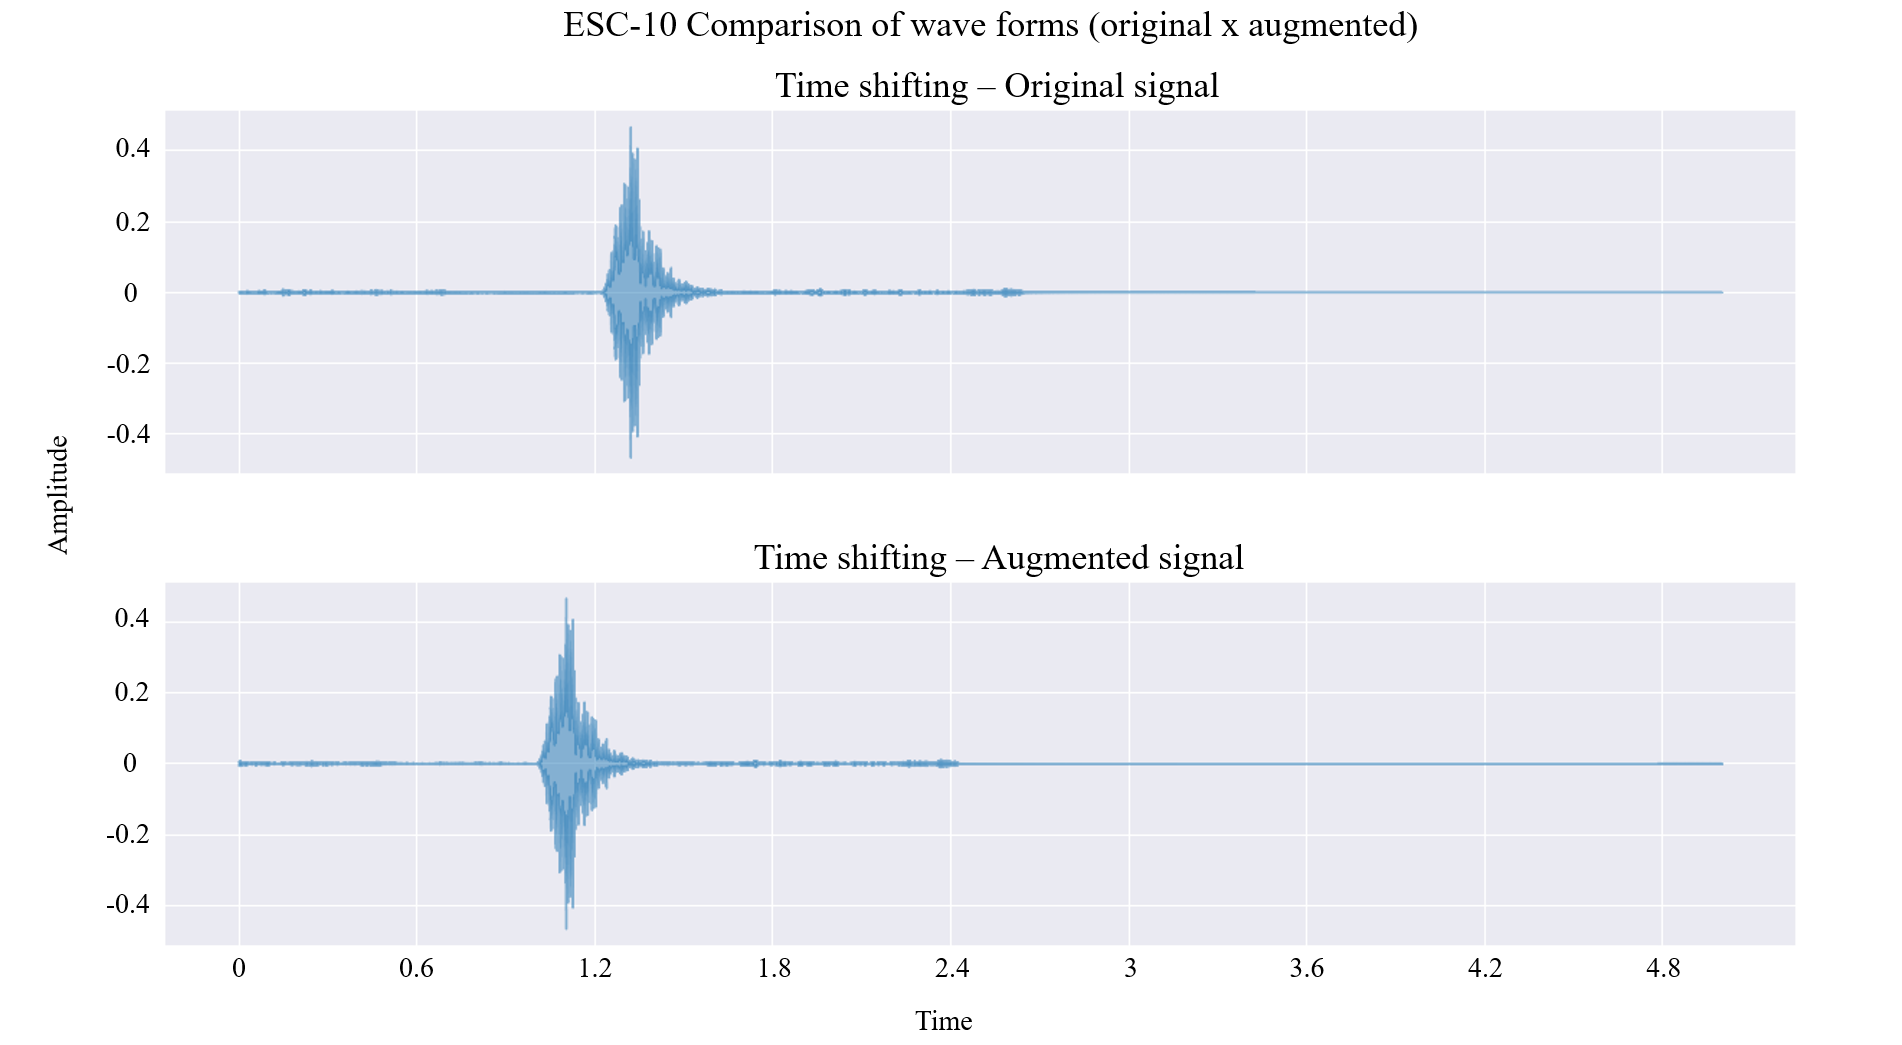
\includegraphics[width=1\textwidth]{resources/images/050-methods/Methods_augmentation_time_shifting.png}
        \smallcaption{Source: Author}
        \label{fig:methods_augmentation_time_shifting}
\end{figure}

After the implementation of the five augmentation techniques, the dataset characteristics were changed as described in Table \ref{table:summary_datasets_before_and_after_augmentation} comparing the values before and after the process.

\begin{table}[ht!]
    \caption[Comparison between the original datasets and their augmented versions]{Characteristics of the datasets before and after the implementation of the augmentation process, including the total size of the compiled features file in format .PKL (Python library Pickle).}
    \label{table:summary_datasets_before_and_after_augmentation}
    \centering
    \begin{tabular}{p{2.7cm}|p{1.6cm}|p{1.7cm}|p{1.7cm}|p{1.6cm}|p{1.7cm}|p{1.7cm}}
        \Xhline{2\arrayrulewidth} 
        \rowcolor{lightgray}
        \textbf{Dataset} & \hfil\textbf{Samples} & \hfil\textbf{Duration} & \hfil\textbf{Features} & \hfil\textbf{Samples} & \hfil\textbf{Duration} & \hfil\textbf{Features}\\
        \rowcolor{lightgray}
          & \hfil (units) & \hfil (h) & \hfil (\gls{m}\gls{b}) & \hfil(units) & \hfil(h) & \hfil(MB)\\    
        \Xhline{2\arrayrulewidth}
        \rowcolor{gray!20} & \multicolumn{3}{c|}{\textbf{Before Augmentation}} & \multicolumn{3}{c}{\textbf{After Augmentation}} \\
        \hline
        ESC-10 & \hfil 400 & \hfil 0.55 & \hfil 2.2 & \hfil 2,400 & \hfil 3.33 & \hfil 1,213\\
        BDLib2 & \hfil 180 & \hfil 0.50 & \hfil 155.6 & \hfil 1,080 & \hfil 3.00 & \hfil 1,088\\
        UrbanSound8K & \hfil 8,732 & \hfil 8.75 & \hfil 3,034 & \hfil 52,392 & \hfil 52.20 & \hfil 21,215\\
        \Xhline{2\arrayrulewidth}
    \end{tabular}
    \smallcaption{Source: Author}
\end{table}


\section{FEATURE EXTRACTION}
\label{sec:methods_feature_extraction}

There is a wide range of audio features that can be broadly categorized into perceptual and physical features based on their semantic interpretation as described in section \ref{subsec:audio_fundamentals_audio_features}. Perceptual features, such as pitch, loudness, rhythm, and timbre, approximate properties that are perceived by human listeners. Conversely, physical features describe audio signals in terms of mathematical, statistical, and physical properties, and are further classified as temporal features and spectral features, based on the domain of representation \cite{Lhoest2021}. Classical machine learning classifiers typically require the extraction of diverse features from the raw audio signal. While it is possible to input raw audio into classifiers based on CNN models, such classifiers tend to have numerous layers and a substantial number of parameters. This is because CNN models must learn to extract features from the raw audio in the early layers \cite{Chu2023}.

This section introduces the physical features and their extraction process utilized during the implementation of the experiments. The process of selecting features tailored to specific classification task is referred in the literature as feature engineering. All of the hereafter audio features are extracted using \index{Librosa}Librosa \cite{McFee2015librosa_sw} due its variety of tools for feature extraction, easy-to-use implementation, supporting for ARM-based processors, and seamless integration with the Python library \index{scikit-learn}scikit-learn \cite{scikitle61}.

Once the audio features have been thoughtfully selected, these "handcrafted features" can be used in both machine learning and neural network classifiers instead of the raw audio, allowing the utilization of a smaller model that is more suitable for embedded devices.

For the purposes of comparison, the feature extraction process of the audio files in the datasets was divided into two methods. The first method (Figure \ref{fig:methods_feature_extraction_leap_window}) employed a sliding or leap window, following the procedures described by \textcite{Silva2019} and \textcite{Lhoest2021} in section \ref{sec:methods_normalization}, as a normalization technique (frame-level normalization). The choice of a sampling rate of 22,050 \gls{hz} was based on the work of \textcite{Salamon2017}, and although \textcite{PiczakESC2015} and \textcite{Bountourakis2015} utilized a sampling rate of 44,100 \gls{hz}, preliminary experiments showed no significant benefits of using a higher sampling rate, and the downturn of such choice was a larger compiled features file that ultimately consumed more memory allocation and longer training time. The choice of around 1 \gls{s} leap window with 50\% overlap was based on the fact that the sounds within the datasets, while non-stationary, did not exhibit abrupt changes over time. Larger leap window sizes, although slightly beneficial in terms of accuracy \cite{Salamon2017}, were not considered. 

\begin{figure}[htbp]
    \raggedright
        \caption{Frame level normalization and feature extraction for a sample of the dataset ESC-10 (5 \gls{s} duration, with 9 windows and 44 frames on each window).}
        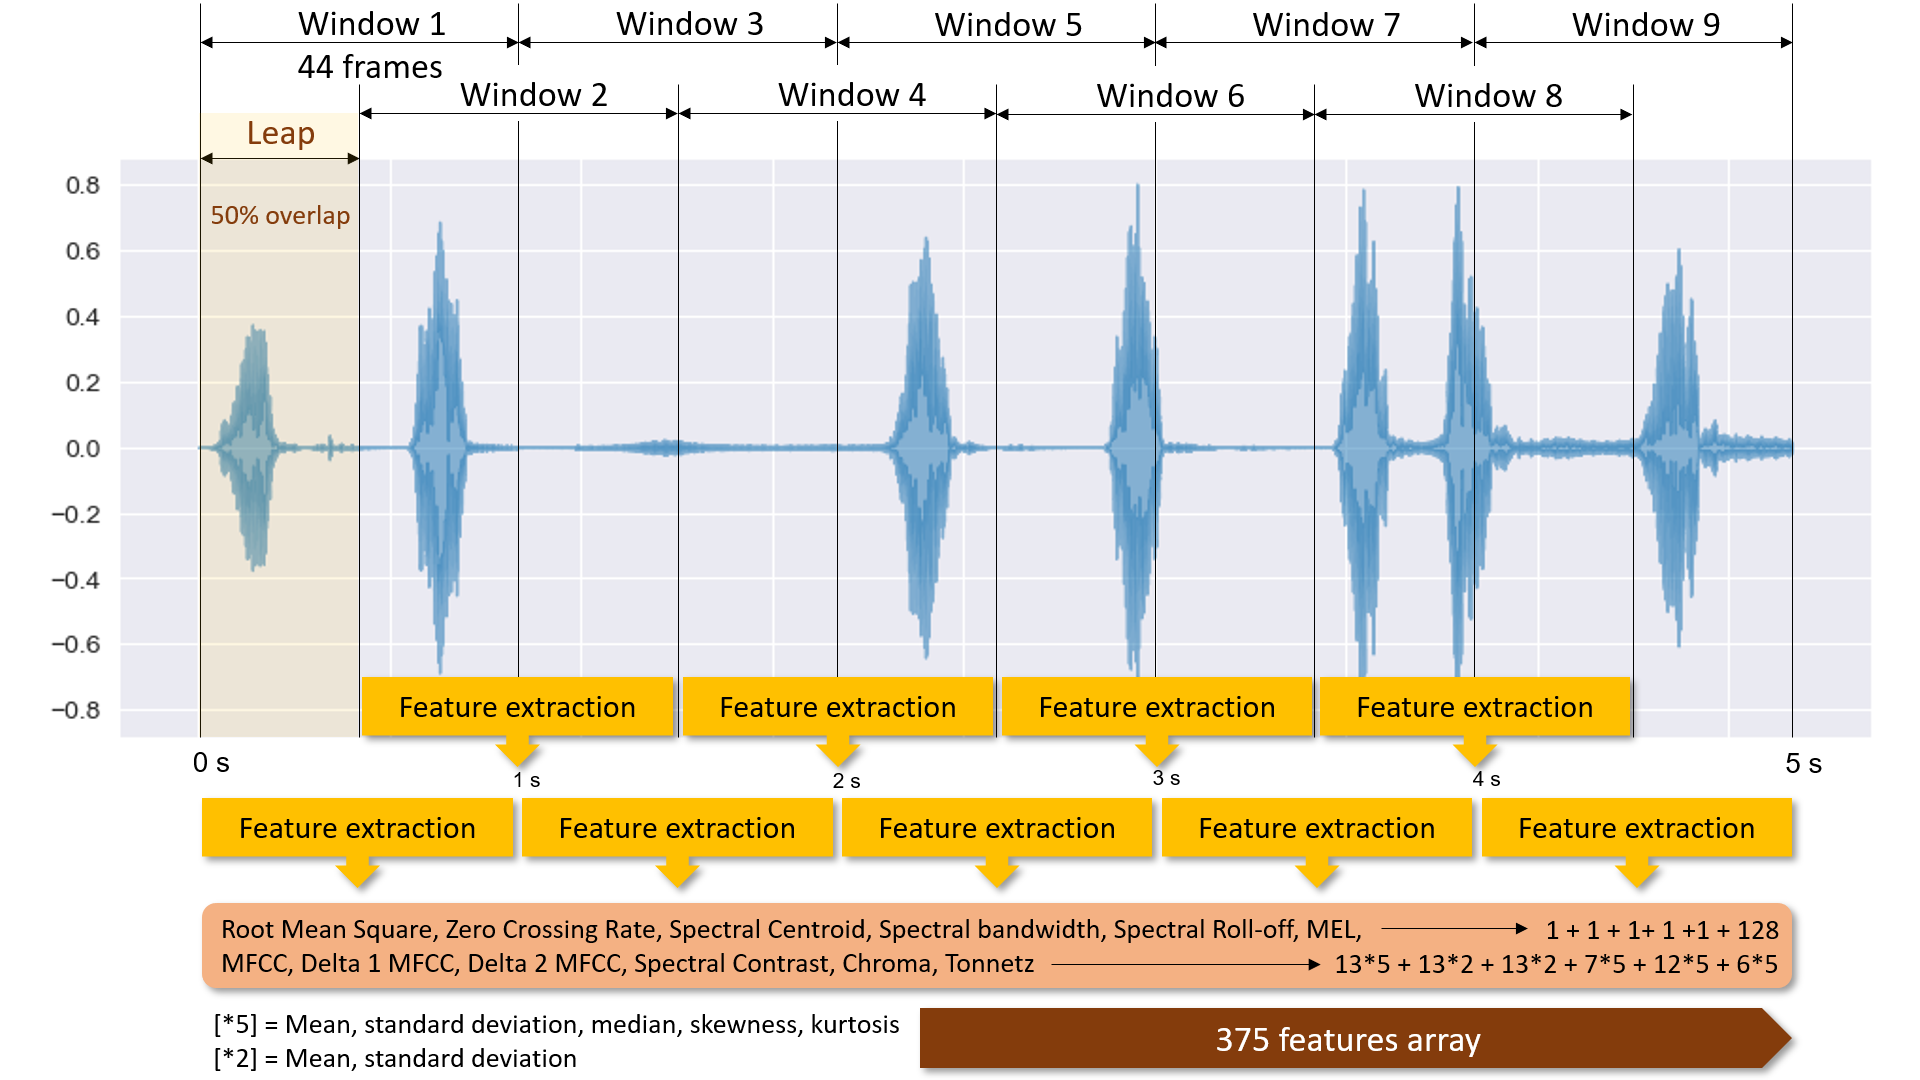
\includegraphics[width=1\textwidth]{resources/images/050-methods/Methods_feature_extraction_1_BDLib2.png}
        \smallcaption{Source: Author}
        \label{fig:methods_feature_extraction_leap_window}
\end{figure}

The second method, involved using the entire audio file (single window) as input for the feature extraction process (Figure \ref{fig:methods_feature_extraction_single_window}), as proposed by the authors of the datasets ESC-10 \cite{PiczakESC2015}, BDLib2 \cite{Bountourakis2015}, and UrbanSound8K \cite{Salamon2017}, but for normalization purposes, utilized the same sampling rate of 22,050 \gls{hz} of the first method. \Textcite{Vandendriessche2021} also utilized the same method in his \gls{cnn} classifier embedded in \gls{fpga}s and \gls{tpu}s.


\begin{figure}[htbp]
    \raggedright
        \caption{Single window or complete audio feature extraction for a sample of the dataset ESC-10 (5 \gls{s} duration, with 1 window and 216 frames).}
        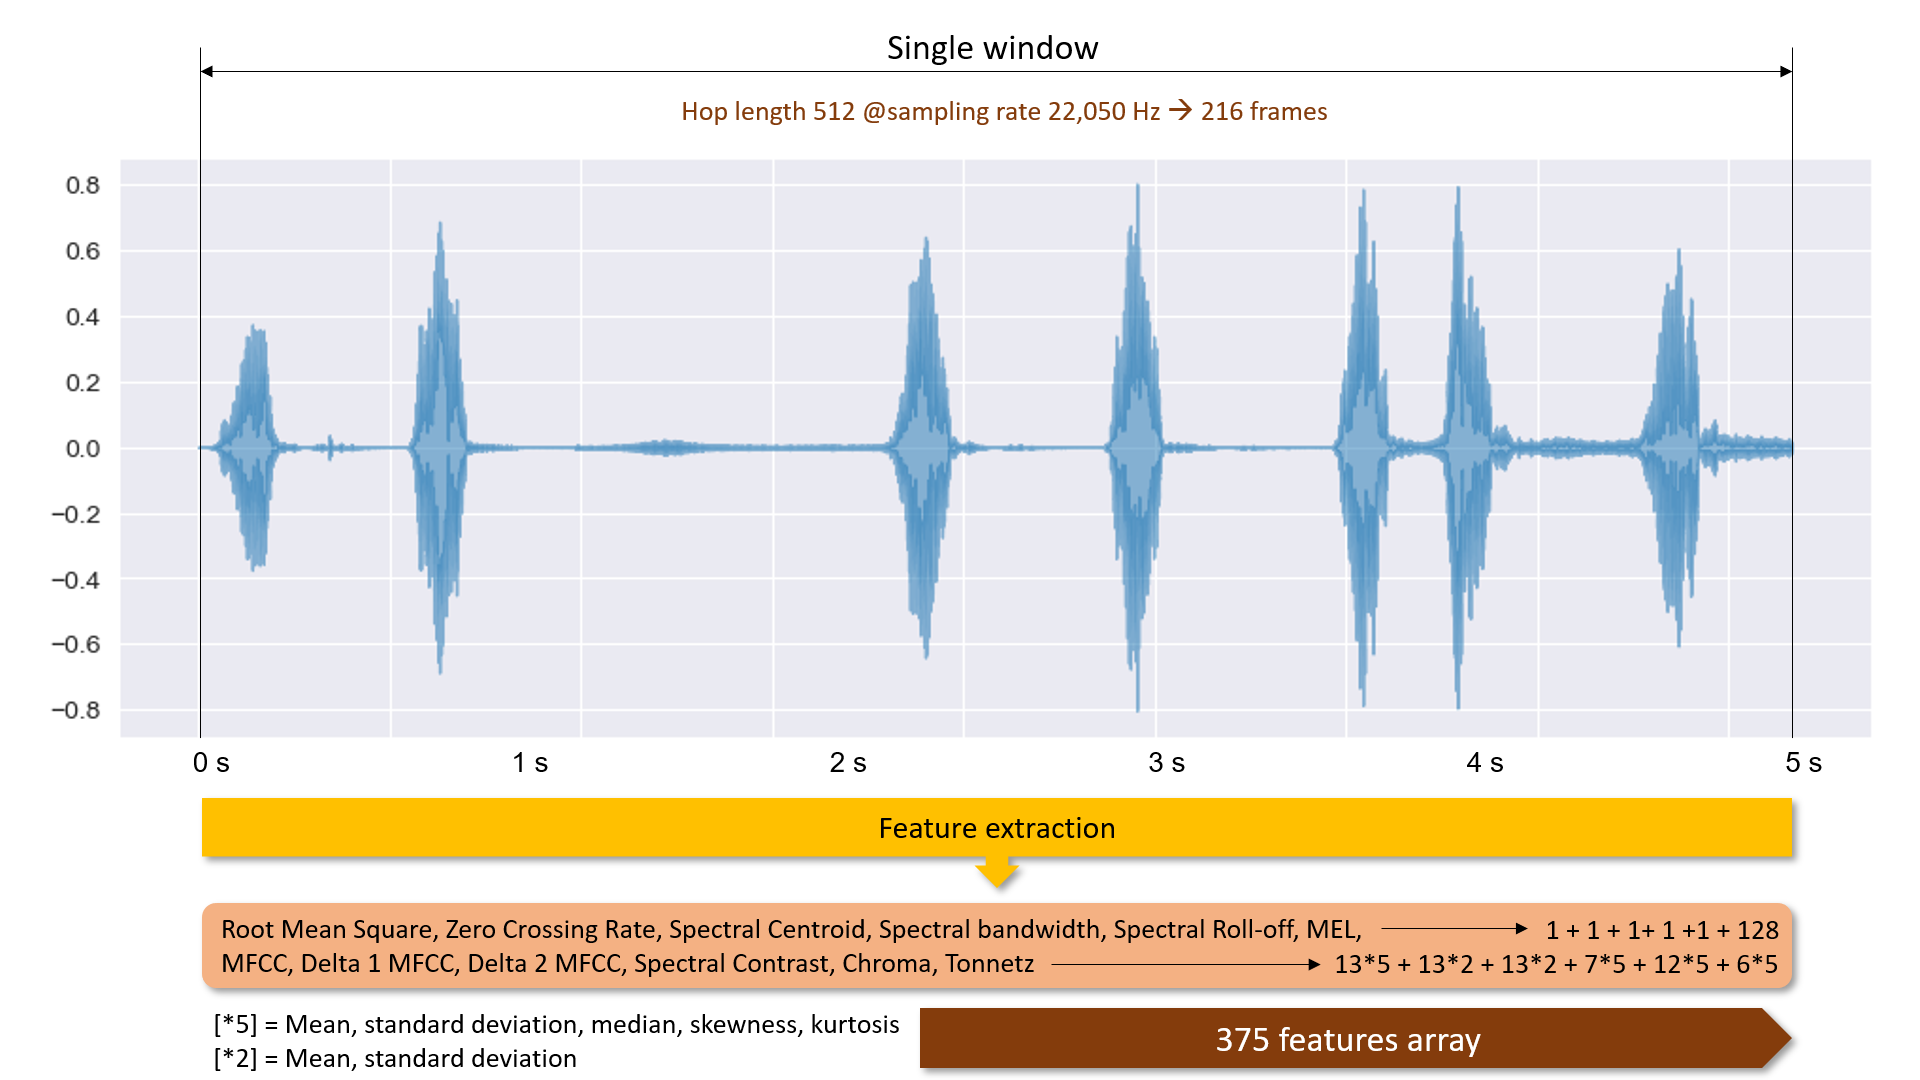
\includegraphics[width=1\textwidth]{resources/images/050-methods/Methods_feature_extraction_2_BDLib2.png}
        \smallcaption{Source: Author}
        \label{fig:methods_feature_extraction_single_window}
\end{figure}

The features selected were defined in the section \ref{subsec:audio_fundamentals_audio_features}, and the feature extraction process utilized a Hann window \cite{Blackmann1958}, with a hop length of 512, sampling rate of 22,050 \gls{hz} and frame size of 1,024 (around 46 ms) for \gls{rms} and \gls{zcr} to achieve a higher time resolution, and $n\_fft$ (number of frames for the \gls{stft}) of 2,048 for the remaining features to increase the frequency resolution. The number of Mel was 128 and \gls{mfcc} was 13.

In the first method, since the number of frames and hop length is fixed, resulting in a window of 1 \gls{s} with 50\% overlapping, the number of windows for the feature extraction on each dataset is calculated by $N_w = audioduration * 2 -1$, leading to 9 windows for the ESC-10, 19 windows for the BDLib2 and 7 windows for the \gls{us8k}.

In both methods, the features with only one coefficient had their per-frame values calculated by mean, on the other hand, the features containing more than one coefficient, had their per-frame values for each coefficient summarized across time using statistics, namely: mean, median, \gls{std}, skewness and kurtosis. The exceptions were Mel with only mean, Delta \gls{mfcc} and Delta-Delta \gls{mfcc} with mean and \gls{std} calculated.  The result was an array containing 375 features as shown in Table \ref{table:features_array_composition}.

\begin{table}[ht!]
    \caption[Composition of the first features array]{Composition of the features array utilized in the machine learning, \gls{ann}, and \gls{cnn} 1D classifiers after the feature extraction process.}
    \label{table:features_array_composition}
    \centering
    \begin{tabular}{p{3cm}|p{2.5cm}|p{1.2cm}|p{1.9cm}|p{3.5cm}|p{1.3cm}}
        \Xhline{2\arrayrulewidth} 
        \rowcolor{lightgray}
        \textbf{Feature} & \hfil\textbf{Coefficients} & \hfil\textbf{Mean} & \hfil\textbf{Mean, \gls{std}} & \textbf{Mean, \gls{std}, median, skewness, kurtosis} & \hfil\textbf{$\sum{}$}\\
        \Xhline{2\arrayrulewidth}
        \gls{rms} & \hfil 1 & \hfil 1 & \hfil --- & \hfil --- & \hfil 1 \\
        \gls{zcr} & \hfil 1 & \hfil 1 & \hfil --- & \hfil --- & \hfil 1 \\
        \gls{sc} & \hfil 1 & \hfil 1 & \hfil --- & \hfil --- & \hfil 1 \\
        \gls{sb} & \hfil 1 & \hfil 1 & \hfil --- & \hfil --- & \hfil 1 \\
        \gls{srp} & \hfil 1 & \hfil 1 & \hfil --- & \hfil --- & \hfil 1 \\
        Mel & \hfil 128 & \hfil 1 & \hfil --- & \hfil --- & \hfil 128 \\
        $\triangle$ \gls{mfcc} & \hfil 13 & \hfil --- & \hfil 2 & \hfil --- & \hfil 26 \\
        $\triangle\triangle$ \gls{mfcc} & \hfil 13 & \hfil --- & \hfil 2 & \hfil --- & \hfil 26 \\
        \gls{mfcc} & \hfil 13 & \hfil --- & \hfil --- & \hfil 5 & \hfil 65 \\
        \gls{sct} & \hfil 7 & \hfil --- & \hfil --- & \hfil 5 & \hfil 35 \\
        Chroma & \hfil 12 & \hfil --- & \hfil --- & \hfil 5 & \hfil 60 \\
        Tonnetz & \hfil 6 & \hfil --- & \hfil --- & \hfil 5 & \hfil 30 \\
        \hline       
        \rowcolor{gray!20} 
        \textbf{Total} & \multicolumn{4}{c|}{} & \hfil\textbf{375} \\
        \Xhline{2\arrayrulewidth}
    \end{tabular}
    \smallcaption{Source: Author}
\end{table}


Finally, a dedicated algorithm was implemented to extract log-mel spectrograms for the \gls{cnn} 2D model. This approach leverages the well-documented strengths of convolutional neural networks in two-dimensional image classification tasks by utilizing a pseudo-image format based on log-mel spectrograms, aggregated with their first and second derivatives, known as Delta and Delta-Delta, respectively. The log-mel spectrogram provides a visual representation of an audio signal's frequency content over time, computed using \gls{stft} and triangular filters. In this representation, the frequency axis (Y-axis) is scaled according to the mel scale, which approximates human auditory perception \cite{Moore2013}, while the amplitude values are converted to a logarithmic scale. The shape of the pseudo-image is contingent upon the audio duration, represented by the number of frames containing the audio samples. For the sliding window method, the number of frames (X-axis) is fixed at 44 frames (equivalent to 1 \gls{s} of audio). For the single window method, it varies according to the audio duration: 173 frames for \gls{us8k} and US8K\_AV (4 \gls{s}), 216 frames for ESC-10 (5 \gls{s}), and 413 frames for BDLib2 (10 \gls{s}). In both methods, the number of mel bands was set to 60, resulting in log-mel spectrogram dimensions of 60 x 173, 60 x 216, and 60 x 431 respectively. For the sliding window method, the dimension remains consistent at 60 x 44 across all datasets.

The first and second derivatives are computed to capture temporal dynamics and spectral acceleration changes, while retaining identical dimensions as the original log-mel spectrogram. These three arrays are subsequently stacked along the frequency band axis, producing a composite array with dimensions of 180 x 44 when considering the sliding window method as depicted in Figure \ref{fig:methods_feature_extraction_log-mel_spectrogram}. By feeding this pseudo-image into the \gls{cnn} 2D model, the resultant feature map encapsulates both static spectral properties and dynamic temporal variations, thereby enhancing the discriminative power of this classifier.

\begin{figure}[htbp]
    \raggedright
        \caption{Log-mel spectrogram aggregated with first and second derivatives for a sample of the dataset US8K (sliding window with 1 \gls{s} duration and 44 frames).}
        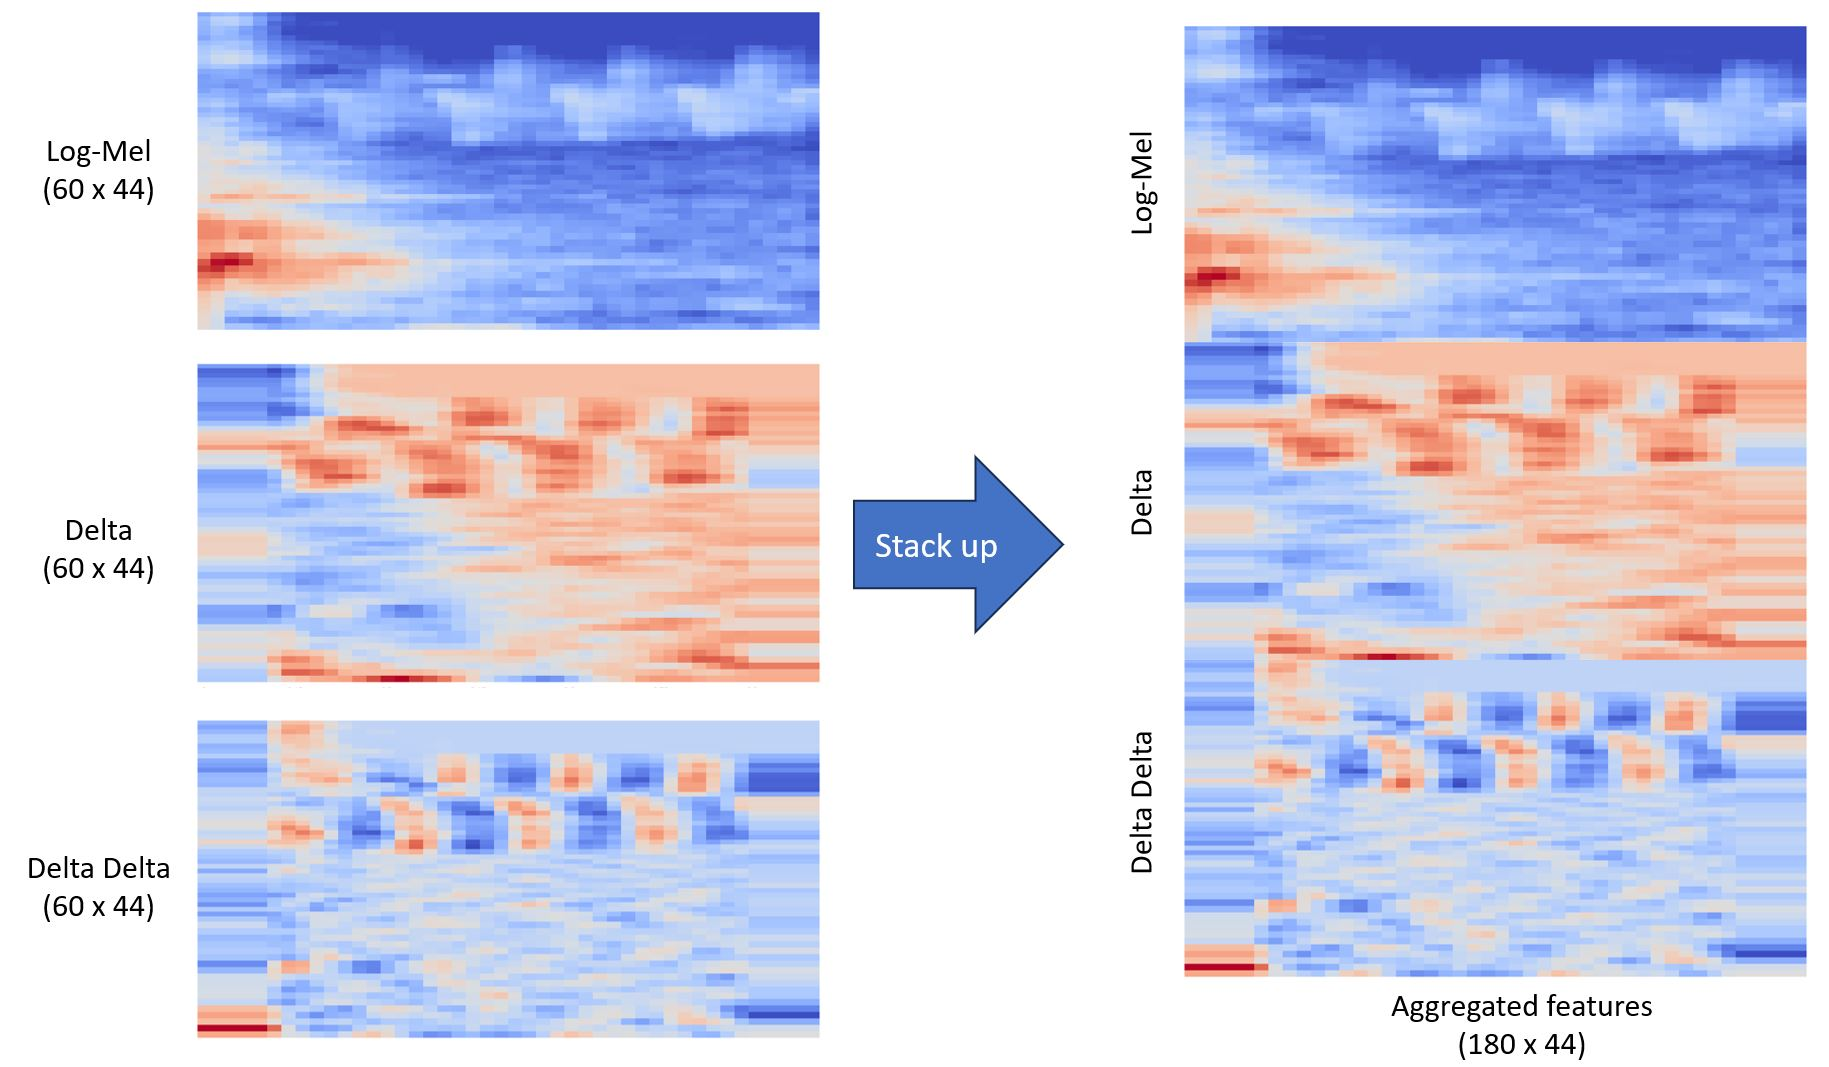
\includegraphics[width=1\textwidth]{resources/images/050-methods/Methods_feature_extraction_3_US8K.jpg}
        \smallcaption{Source: Author}
        \label{fig:methods_feature_extraction_log-mel_spectrogram}
\end{figure}

\section{TRAINING THE CLASSIFIERS}
\label{sec:methods_training_classifiers}

The initial step on training the models involved finding the best \index{hyperparameter}hyperparameters using grid search and built-in cross-validation \index{scikit-learn}\cite{scikitle61} to optimize model performance. Grid search systematically explored a predefined hyperparameter grid, testing various combinations to identify the set that yields the best performance while built-in cross-validation was employed to assess model generalization by dividing the dataset into multiple subsets. The use of built-in cross-validation helps mitigate overfitting by providing a more robust estimate of the model performance across different data subsets, ensuring that the selected hyperparameters are likely to perform well on unseen data.

By default, the grid search splits the dataset into training and testing sets according to the parameter $cv$ (number of cross-validations), and the model is trained on the former and evaluated on the latter, repeatedly, for each combination of hyperparameters in the grid. Depending on the number of hyperparameters to be searched, this process may take a long time of execution, specially in neural networks, and therefore, although recommended in the general literature to run the built-in cross-validation with 10 sets, it was established the number of 5 sets for all models, hence 80\% for training and 20\% for testing. Once the set of optimal hyperparameters was found for each model, the final step of the training started, validating the model on a separate, unseen validation set, using the method of k-fold cross-validation, to assess its true generalization performance. 

Each of the aforementioned datasets was initially intended to undergo validation using k-fold cross-validation methods, with each dataset considering a distinct value for k: ESC-10 employs 5 folds, BDLib2 utilizes 3 folds, and UrbanSound8K employs 10 folds. Figure \ref{fig:methods_training_k-fold} illustrates the process of the k-fold cross-validation using the ESC-10 dataset as example, demonstrating that each k-fold (0 to 4) assigned in the dataset metadata was properly separated within the 10 classes. In order to compare the classifier's results accordingly, the number of k-folds for each dataset was respected.

In the end of this process, the classifiers' models using machine learning techniques and ensemble methods were configured with their standard parameters according to the \index{scikit-learn}scikit-learn library, except for the following \index{hyperparameter}hyperparameters:

\begin{itemize}
    \item \gls{gnb}: $ priors$ = none (Prior probabilities of the classes);
    \item \gls{svm}: $kernel$ = 'linear', $C$ = 0.50 (Regularization parameter);
    \item \gls{lr}: $solver$ = 'saga', $C$ = 0.50 (Regularization parameter), $max\_iter$ = 500 (Maximum number of iterations taken for the solver to converge);
    \item \gls{k-nn}: $n\_neighbors$ = 3, $metric$ = 'minkowski', $p$ = 2 (Power parameter for the Minkowski metric, 2 means euclidean distance), $leaf\_size$ = 20 (Leaf size passed to BallTree or KDTree algorythm to calculate the nearest neighbors considered that 'auto' is the standard);
    \item \gls{rf}: $criterion$ = 'gini', $n\_estimators$ = 500 (The number of trees in the forest), $bootstrap$ = True (Whether bootstrap samples are used when building trees);
    \item Voting: $voting$ = 'soft' (Predicts the class label based on the argmax of the sums of the predicted probabilities).
\end{itemize}

\begin{figure}[htbp]
    \raggedright
        \caption{Process of k-fold cross-validation using the metadata of the dataset ESC-10 with 10 classes and 5 folds.}
        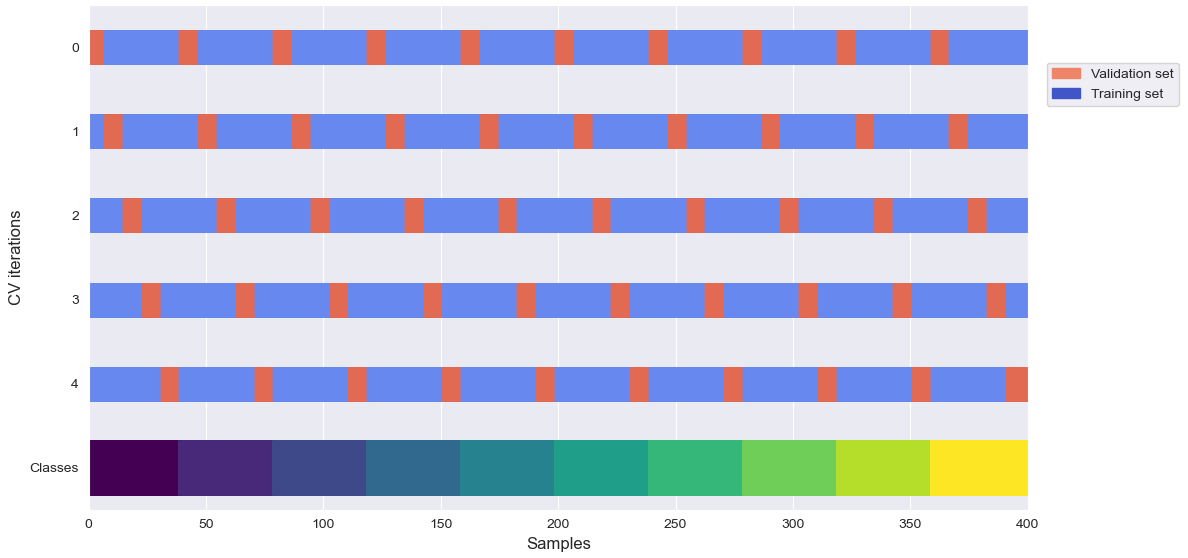
\includegraphics[width=1\textwidth]{resources/images/050-methods/Methods_training_k-fold.png}
        \smallcaption{Source: Author}
        \label{fig:methods_training_k-fold}
\end{figure}

The \gls{ann} was originally created using Kolmogorov's theorem where given any continuous function
$\phi: I^n \longrightarrow \mathbf{R}^m, \phi(\mathbf{x})=\mathbf{y}$, where $I$ is the closed unit interval $[0,1]$ representing the classes, and therefore $I^n$ is the $n$ dimensional unit cube, $\phi$ can be implemented exactly by a 3 layer neural network having $n$ processing elements in the first input layer ($x$), followed by $(2 n+1)$ processing elements (neurons) in the hidden layer, and $m$ processing elements in the output layer ($y$) \cite{Hecht-Nielsen1987}. The network was built using \index{Keras}Keras sequential model to define a \gls{mlp} with the first dense layer receiving as input an array with 375 features (parameterized with \gls{pca} when requested) and \gls{relu} activation function. The second and third dense layers were hidden, with 375 neurons and 750 neurons respectively, both using \gls{relu} activation function. To improve the model accuracy proposed by Hecht-Nielsen, one additional hidden dense layer was added based on the grid search and built-in cross-validation results. A dropout layer with 20\% rate was also added after each hidden layer to improve generalization, prevent overfitting, and make the model more robust by introducing randomness during training.

The final dense layer with 10 neurons (one for each class) is utilized for the classification task by using \textbf{softmax} activation function to assign probabilities to each class in the output layer. The hyperparameters used in the grid search to achieve this model configuration (Figure \ref{fig:methods_training_ANN_architecture} and Figure \ref{fig:methods_training_ANN_architecture_jupyter_notebook}) were $loss$ = 'categorical\_crossentropy', and the Adam optimizer with $learning\_rate$ = 0.0001, $beta\_1$ = 0.5 (The exponential decay rate for the 1\textsuperscript{st} moment estimates), $beta\_2$ = 0.999 (The exponential decay rate for the 2\textsuperscript{nd} moment estimates), $epsilon$ = 1e-07 (A small constant for numerical stability), $amsgrad$ = True (Whether to apply AMSGrad variant \cite{Reddi2018} of this algorithm). 


\begin{figure}[htbp]
    \raggedright
        \caption{ANN architecture utilized in the experiments.}
        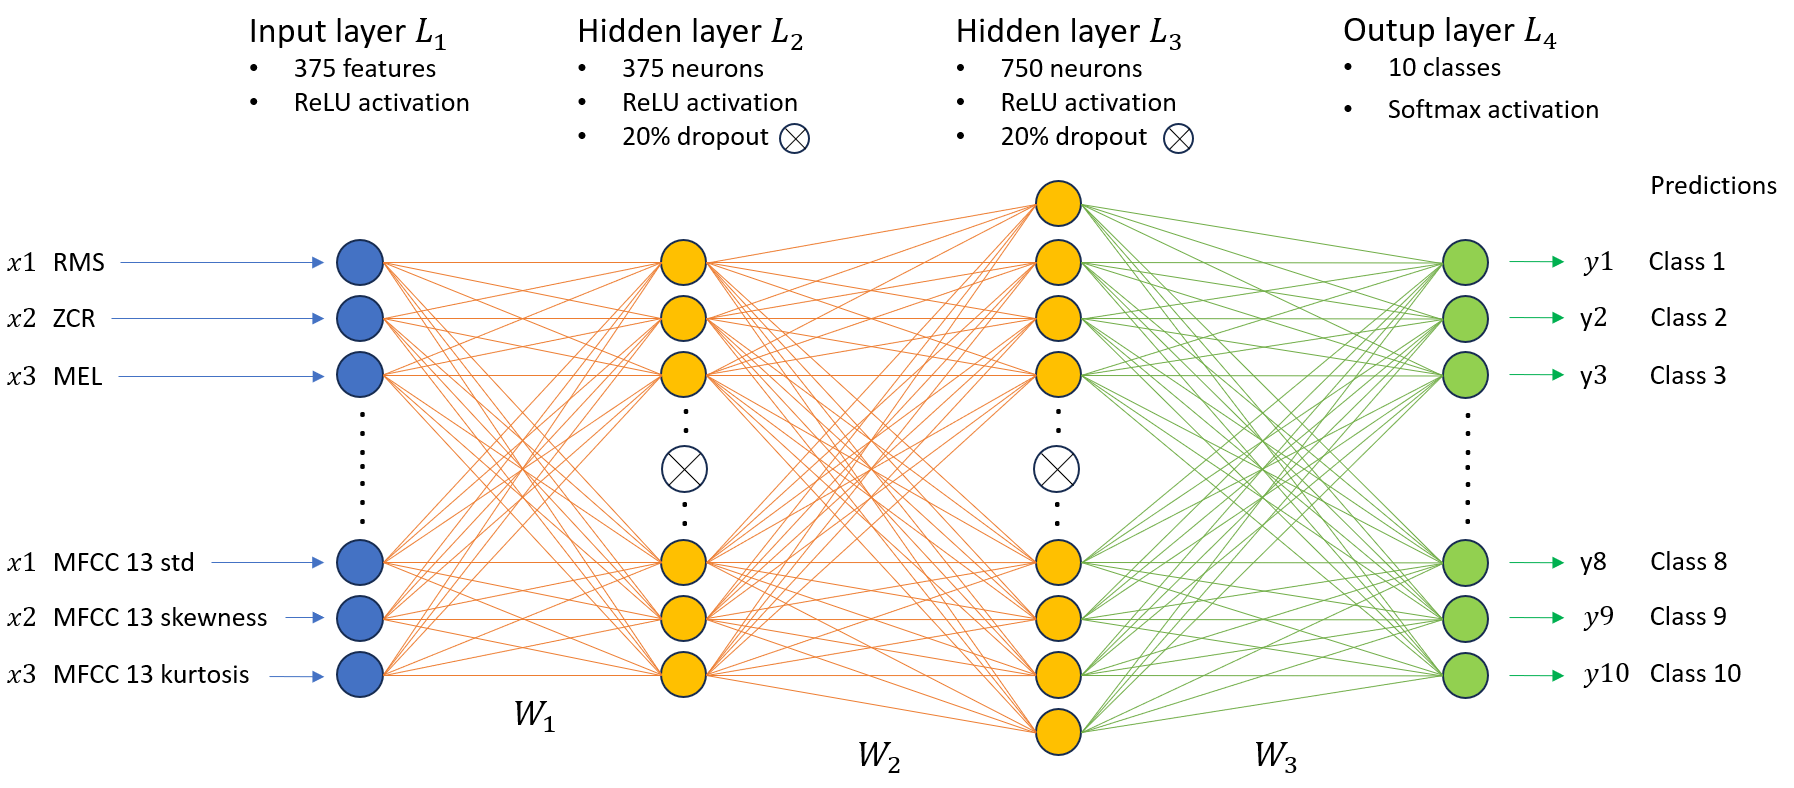
\includegraphics[width=1\textwidth]{resources/images/050-methods/Methods_training_ANN_architecture.png}
        \smallcaption{Source: Author}
        \label{fig:methods_training_ANN_architecture}
\end{figure} 


\begin{figure}[htbp]
    \raggedright
        \caption{ANN model summary from Jupyter notebook.}
        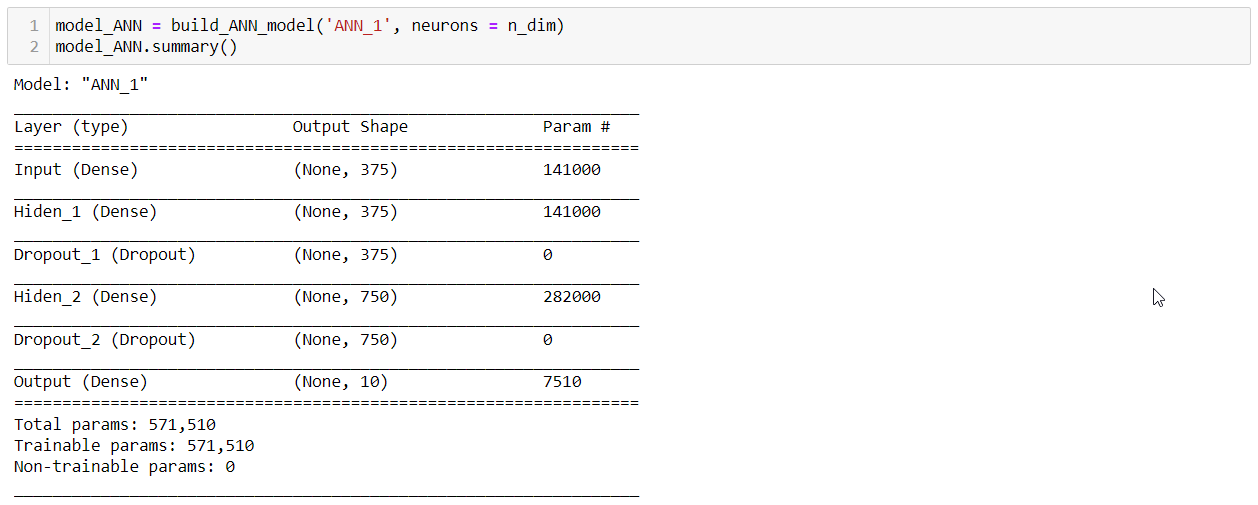
\includegraphics[width=1\textwidth]{resources/images/050-methods/Methods_training_ANN_architecture_jupyter_notebook.png}
        \smallcaption{Source: Author}
        \label{fig:methods_training_ANN_architecture_jupyter_notebook}
\end{figure} 


A second round of grid search was performed to find the best parameters for the batch size and epochs, implemented together with a early stop process. Ultimately, the values considered were: $batch\_size = 20$, $epochs$ = 350 and $EarlyStopping$ with $monitor$ = 'val\_accuracy', $min\_delta$ = 0.0001, $patience$ = 150, and $restore\_best\_weights$ = True. As illustrated in Figure \ref{fig:methods_training_ANN_loss_and_accuracy_graphs}, the \gls{ann} model achieved a stable and rather well generalized behavior during the built-in cross-validation process.


\begin{figure}[htbp]
    \raggedright
        \caption{Loss and accuracy graphs of the implemented ANN model.}
        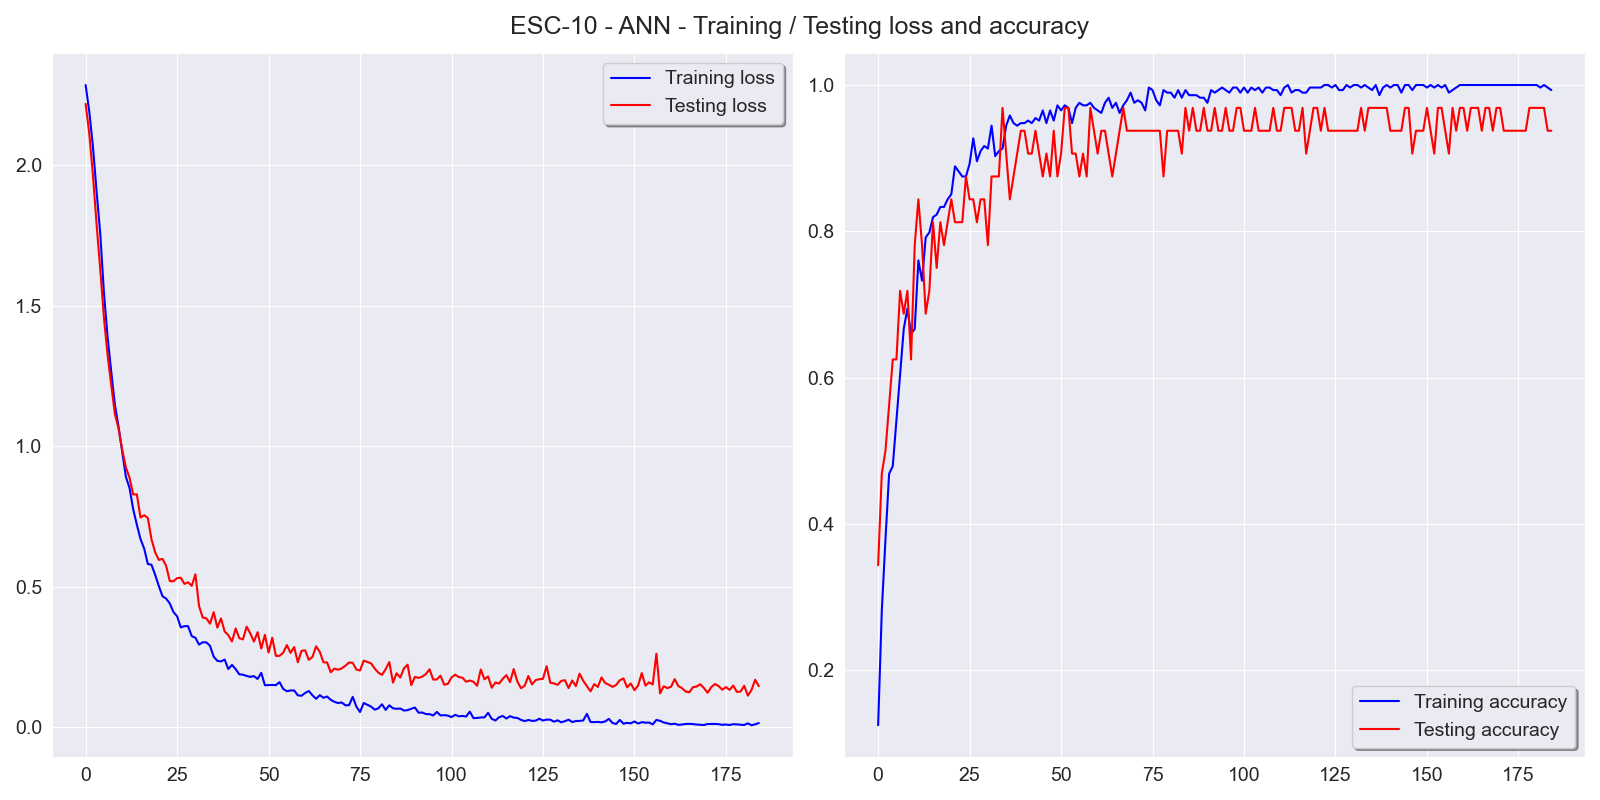
\includegraphics[width=1\textwidth]{resources/images/050-methods/Methods_training_ANN_loss_accuracy.png}
        \smallcaption{Source: Author}
        \label{fig:methods_training_ANN_loss_and_accuracy_graphs}
\end{figure} 

The architecture of the \gls{cnn} 1D model illustrated in Figure \ref{fig:methods_training_CNN_1D_architecture} and summarized by the Jupyter notebook in Figure \ref{fig:methods_training_CNN_1D_architecture_jupyter_notebook} consisted of several layers, compiled with a categorical cross-entropy loss function, adamax optimizer, and accuracy as the evaluation metric:

\begin{figure}[htbp]
    \raggedright
        \caption{CNN 1D architecture utilized in the experiments.}
        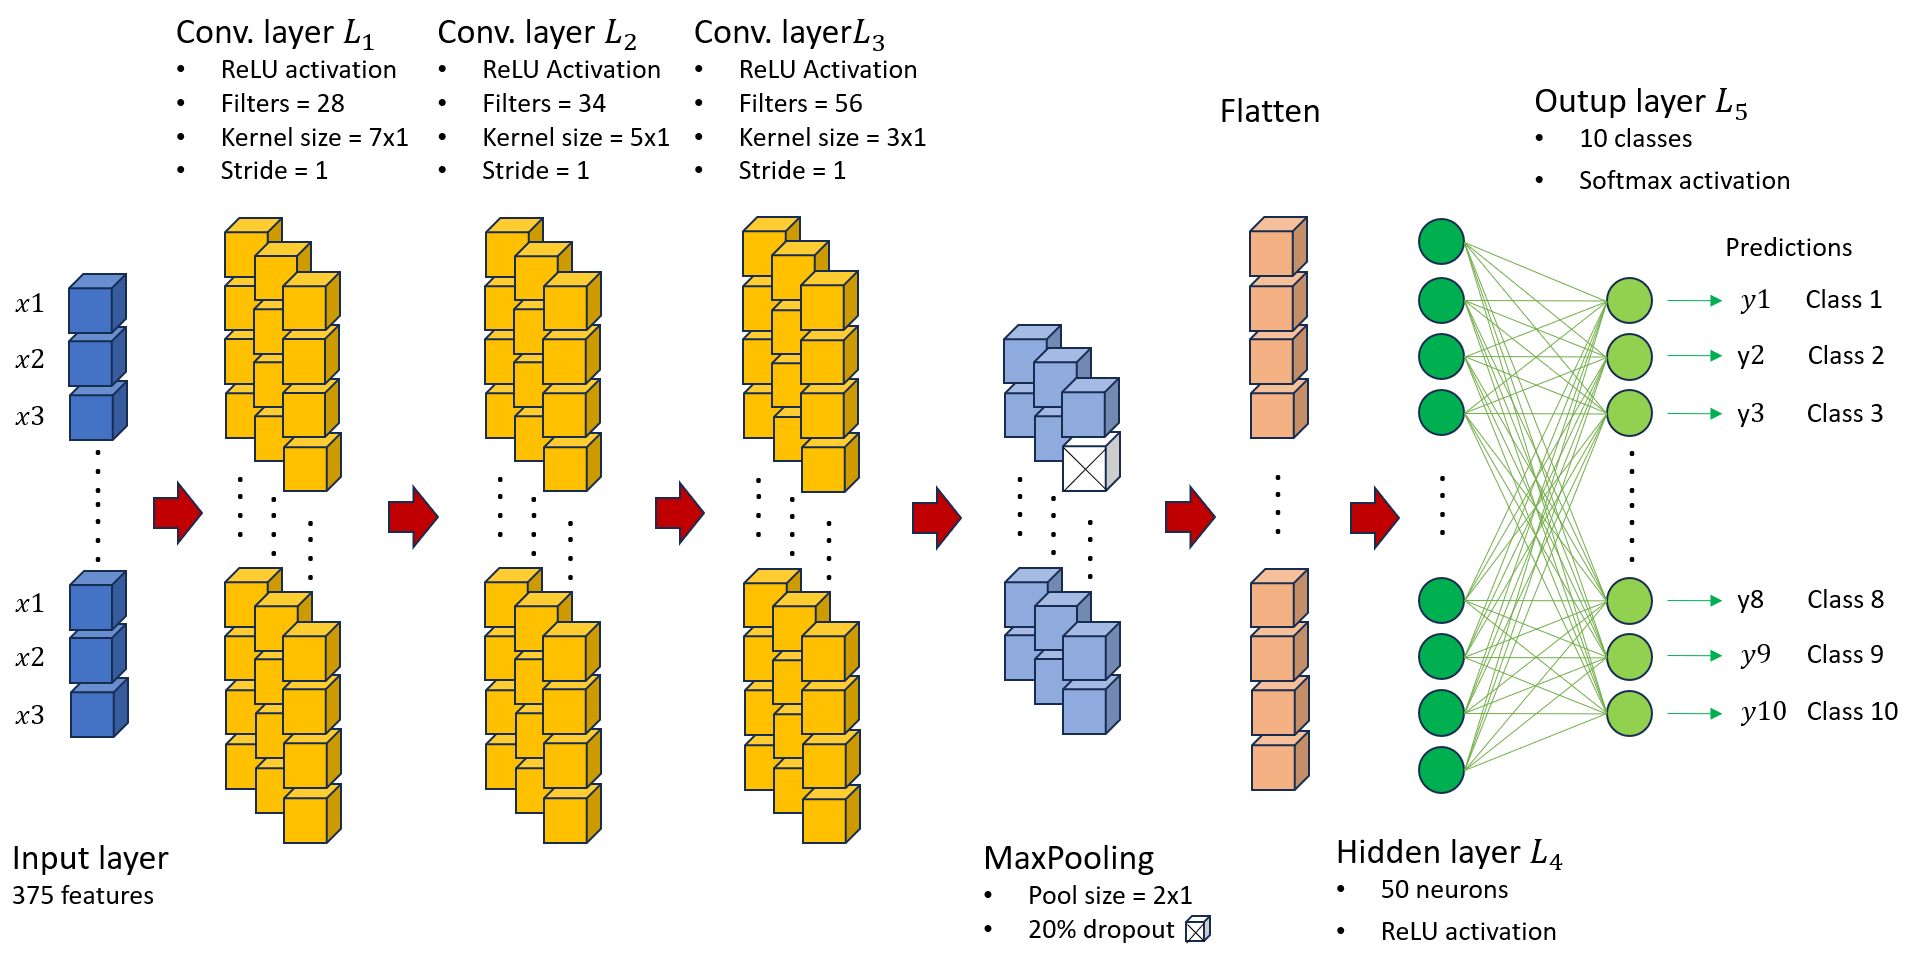
\includegraphics[width=1\textwidth]{resources/images/050-methods/Methods_training_CNN1D_architecture.png}
        \smallcaption{Source: Author}
        \label{fig:methods_training_CNN_1D_architecture}
\end{figure} 

\begin{itemize}
    \item Conv1D\_1: The first convolutional layer has 28 filters with a kernel size of 7 x 1, and it uses the \gls{relu} activation function, receiving as input an array with 375 features;
    \item Conv1D\_2: This is the second convolutional layer with 34 filters, and kernel size of 5 x 1. It also uses the \gls{relu} activation function and applies L2 regularization to the kernel with 0.001 and bias with 0.01. $Padding$ is set to 'same' with $stride$ as default (1) to ensure the output size matches the input size;
    \item Conv1D\_3: This is the last convolutional layer. It has 56 filters with a kernel size of 3 x 1. The same parameters of the second convolutional layer are used for the activation function and L2 regularization to the kernel and bias;
    \item MaxPooling1D\_3: This layer performs max pooling with a pool size of 2 x 1, reducing the dimensionality of the data by taking the maximum value within each window of size 2 x 1;
    \item Dropout\_1: To reduce overfitting, this layer randomly sets 20\% of the input units to 0 at each update during training; 
    \item Flatten\_5: To prepare the data for the next step, this layer reshapes the output of the previous layer into a 1-dimensional vector;
    \item Dense: This layer is a fully connected to the previous layer with 50 neurons; 
    \item Output: Finally, the classification task is performed in this layer. It has a number of neurons equal to the number of output classes (10), and it uses the softmax activation function to output probabilities for each class.
\end{itemize}

\begin{figure}[htbp]
    \raggedright
        \caption{CNN 1D model summary from Jupyter notebook.}
        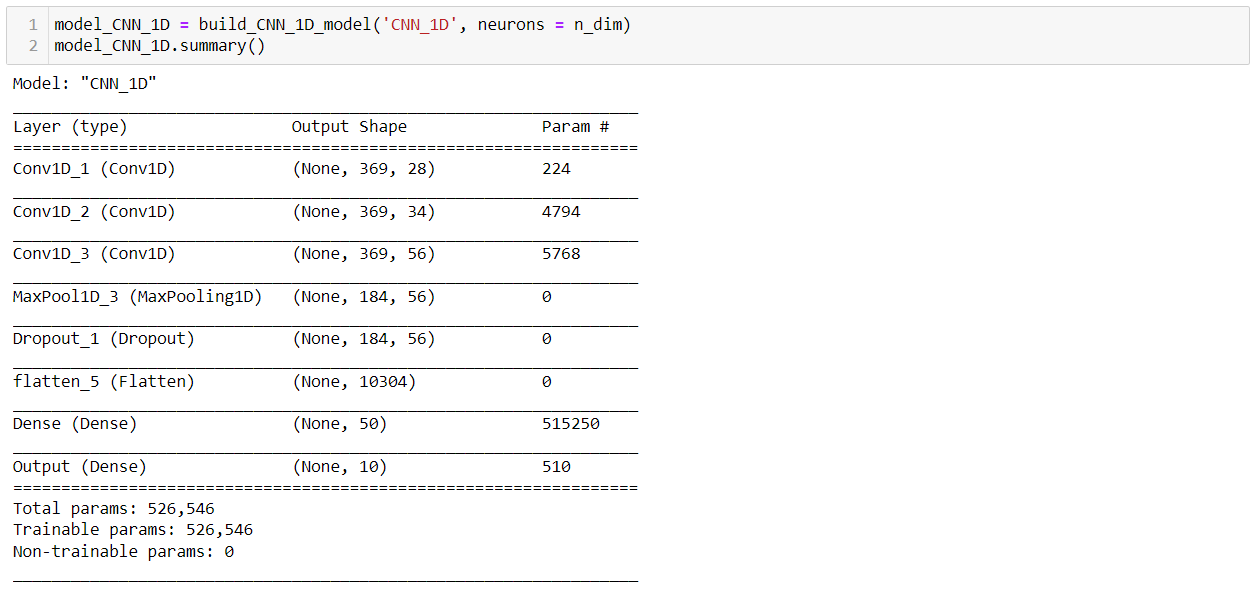
\includegraphics[width=1\textwidth]{resources/images/050-methods/Methods_training_CNN1D_architecture_jupyter_notebook.png}
        \smallcaption{Source: Author}
        \label{fig:methods_training_CNN_1D_architecture_jupyter_notebook}
\end{figure} 

In the same way as the \gls{ann}, a grid search was performed to find the batch size and epochs that yield the highest accuracy, implemented together with a early stop process. In the final stages, the values considered were: $batch\_size = 20$, $epochs$ = 150 and $EarlyStopping$ with $monitor$ = 'val\_accuracy', $min\_delta$ = 0.0001, $patience$ = 50, and $restore\_best\_weights$ = True. Figure \ref{fig:methods_training_CNN_1D_loss_and_accuracy_graphs} depicts a robust model that achieved the highest accuracy with just a few epochs. Early stop was triggered during the built-in cross-validation between 50 to 70 epochs.


\begin{figure}[htbp]
    \raggedright
        \caption{Loss and accuracy graphs of the implemented CNN 1D model.}
        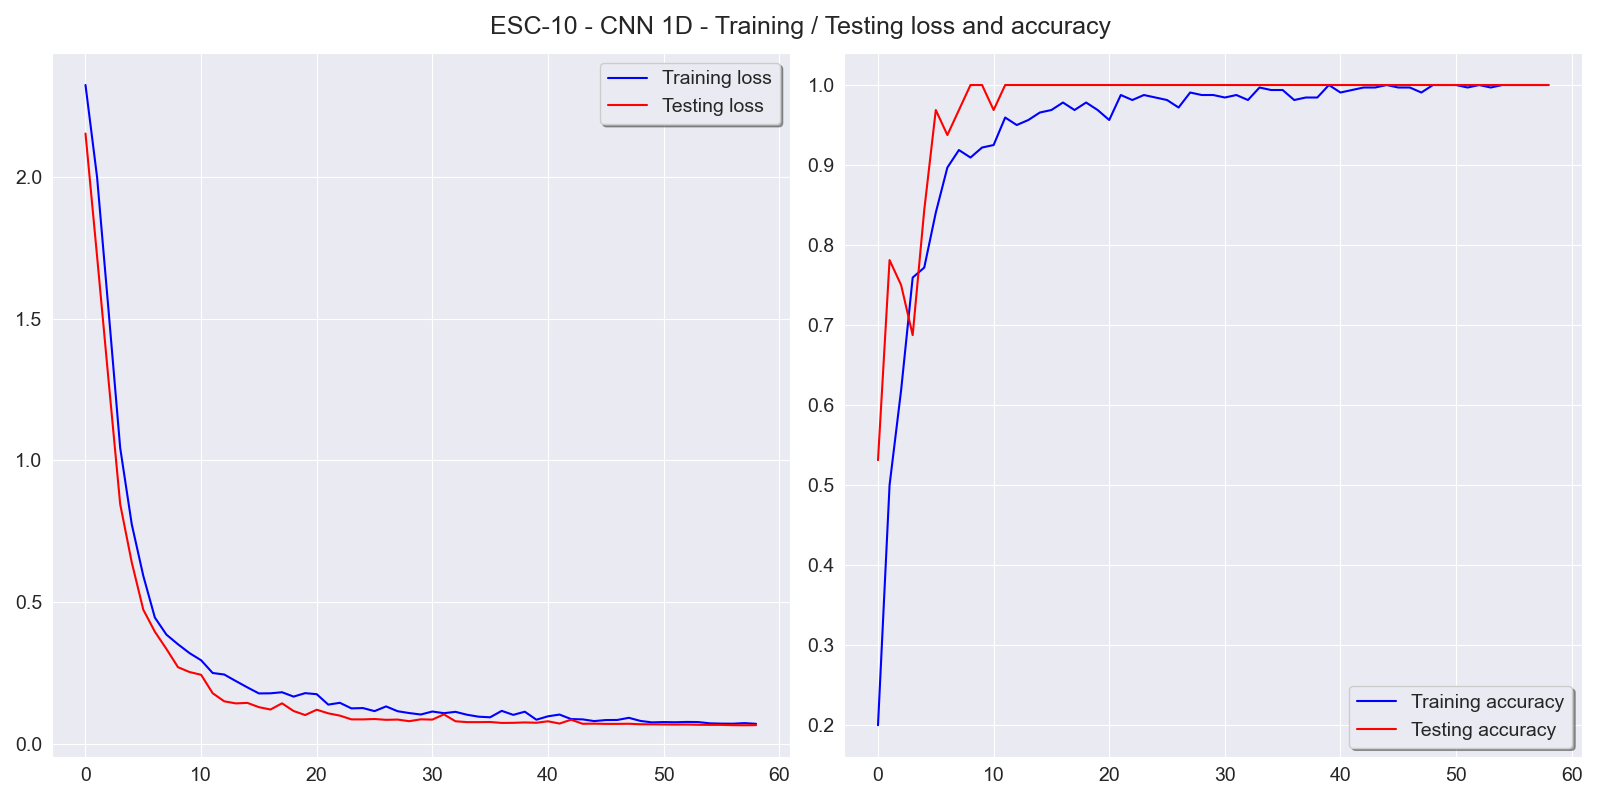
\includegraphics[width=1\textwidth]{resources/images/050-methods/Methods_training_CNN1D_loss_accuracy.png}
        \smallcaption{Source: Author}
        \label{fig:methods_training_CNN_1D_loss_and_accuracy_graphs}
\end{figure} 


During this phase of the study, several architectures for the \gls{cnn} 2D model were examined, including those proposed by \textcite{Piczak2015}, \textcite{Su2020}, \textcite{Luz2021}, and \textcite{Chu2023}. The architecture that exhibited the best performance was adapted from \textcite{Su2020}. However, this model was modified to utilize four convolutional layers, in contrast to the six layers in the original design. Additionally, modifications were made to the stride values in specific layers, and additional dropout layers were incorporated. The final model (Figure \ref{fig:methods_training_CNN_2D_architecture}) was compiled using a categorical cross-entropy loss function, a stochastic gradient descent optimizer (with a learning rate of 0.001 and momentum of 0.9), and accuracy as the evaluation metric:

\begin{figure}[htbp]
    \raggedright
        \caption{CNN 2D architecture utilized in the experiments. Specific illustration for the US8K\_AV dataset.}
        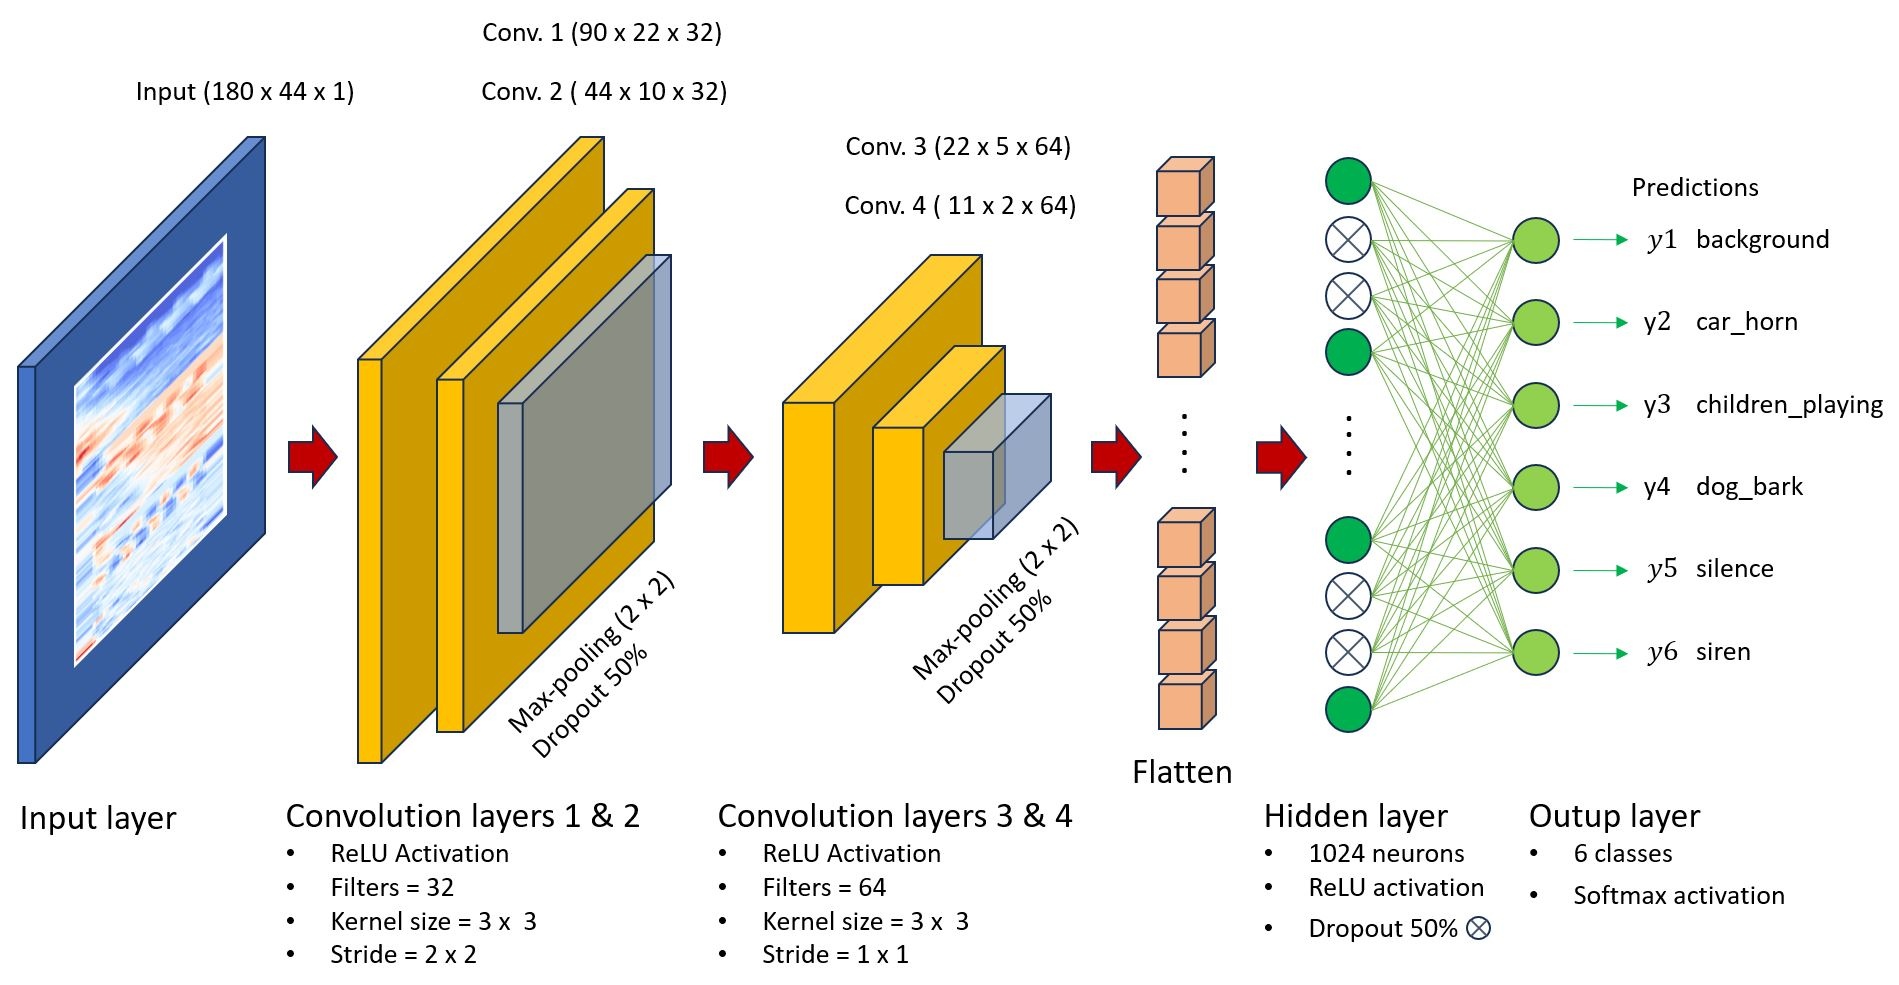
\includegraphics[width=1\textwidth]{resources/images/050-methods/Methods_training_CNN2D_architecture.jpg}
        \smallcaption{Source: Author}
        \label{fig:methods_training_CNN_2D_architecture}
\end{figure} 

\begin{itemize}
    \item The first convolutional layer comprises 32 filters with a kernel size of 3 x 3 and a stride of 2 x 2, utilizing the \gls{relu} activation function, followed by batch normalization;
    \item The second convolutional layer mirrors the first one but is followed by a max-pooling layer with a pool stride of 2 x 2 to reduce the dimensions of the convolutional feature maps and includes a dropout rate of 50\% to mitigate overfitting;
    \item The third convolutional layer consists of 64 filters with a kernel size of 3 x 3 and a stride of 1 x 1, employing the \gls{relu} activation function, followed by batch normalization;
    \item The fourth convolutional layer is identical to the third one but is succeeded by a max-pooling layer with a pool stride of 2 x 2 and a dropout rate of 50\%;
    \item A flatten layer reshapes the output from the previous layer into a one-dimensional vector in preparation for subsequent processing;
    \item A fully connected dense layer with 1,024 neurons is added before the final output, followed by another dropout layer set at 50\%;
    \item The final classification task is performed in the last layer, which contains neurons equal to the number of output classes (10) and uses the softmax activation function to output probabilities for each class;
\end{itemize}

A grid search was conducted to determine the optimal batch size and number of epochs that would yield the highest accuracy. This process was implemented alongside an early stopping mechanism. The implemented parameters were: $batch\_size = 32$, $epochs$ = 100 and $EarlyStopping$ with $monitor$ = 'val\_accuracy', $min\_delta$ = 0.0001, $patience$ = 20, and $restore\_best\_weights$ = True. Figure \ref{fig:methods_training_CNN_2D_loss_and_accuracy_graphs} illustrates that the model continued to learn and may have achieved better performance if trained for additional epochs since early stopping was never triggered during built-in cross-validation. Nonetheless, limiting training to 100 epochs was considered sufficient for this study.


\begin{figure}[htbp]
    \raggedright
        \caption{Loss and accuracy graphs of the implemented CNN 2D model}
        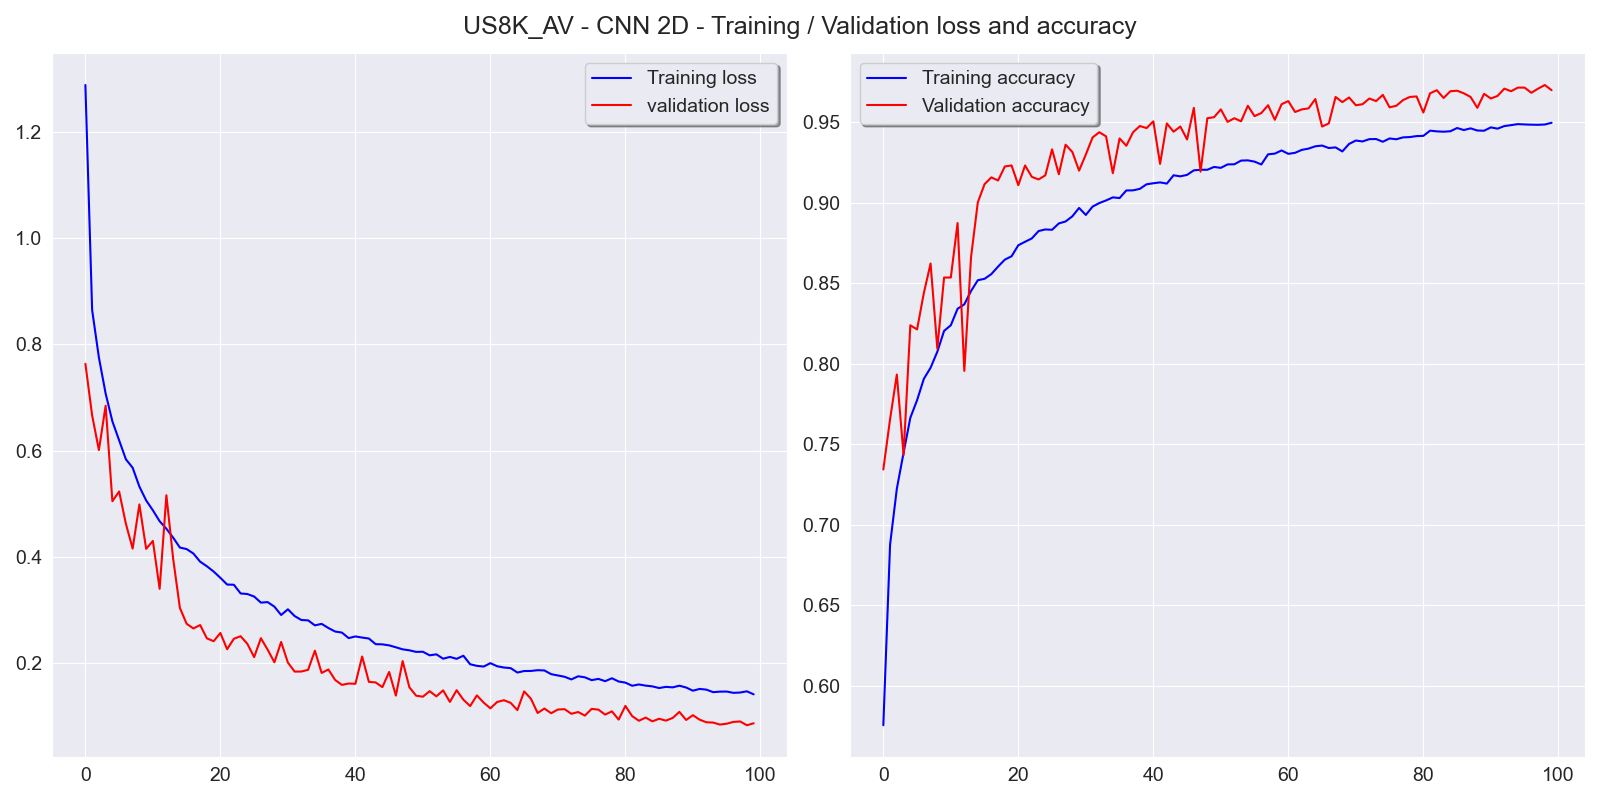
\includegraphics[width=1\textwidth]{resources/images/050-methods/Methods_training_CNN2D_loss_accuracy.png}
        \smallcaption{Source: Author}
        \label{fig:methods_training_CNN_2D_loss_and_accuracy_graphs}
\end{figure} 


\section{EVALUATION}
\label{sec:methods_evaluation}

Once the training is completed, the evaluation phase started, initially stationary as illustrated in the methodology diagram (Training / Classification flow), and lastly mobile (Evaluation flow), in the practical scenario of a regular passenger vehicle, considering factors like ambient noise, changing environmental conditions, and the need for instantaneous responses.

The C-Bots utilized in the living laboratory are equipped with ReSpeaker Mic Array v2.0 \cite{ReSpeake72} installed in the avatar head (Figure \ref{fig:methods_evaluation_AVATAR_ReSpeaker}), connected to the AVATAR \gls{ecu} which is used for speech recognition among other functions. The ReSpeaker contains 4 high performance digital microphones (ST MP34DT01TR-M), with sensitivity of -26 \gls{db}FS (Omnidirectional), acoustic overload point of 120 \gls{db} \gls{spl}, maximum sampling rate of 16 \gls{k}\gls{hz}, and speech recognition algorithm on-chip, including support to far-field voice capture. The AVATAR \gls{ecu} is a Raspberry Pi connected to the vehicle \gls{ee} architecture via \gls{can} and Ethernet, and according to the C-Bot system engineer, the \gls{esr} algorithm could be implemented on this module or in another high-performance computing module of the vehicle, and its output information published via ROS2. 

\begin{figure}[htbp]
    \raggedright
        \caption{Illustration of the ReSpeaker Mic Array v2.0 installed in the AVATAR of the C-Bot.}
        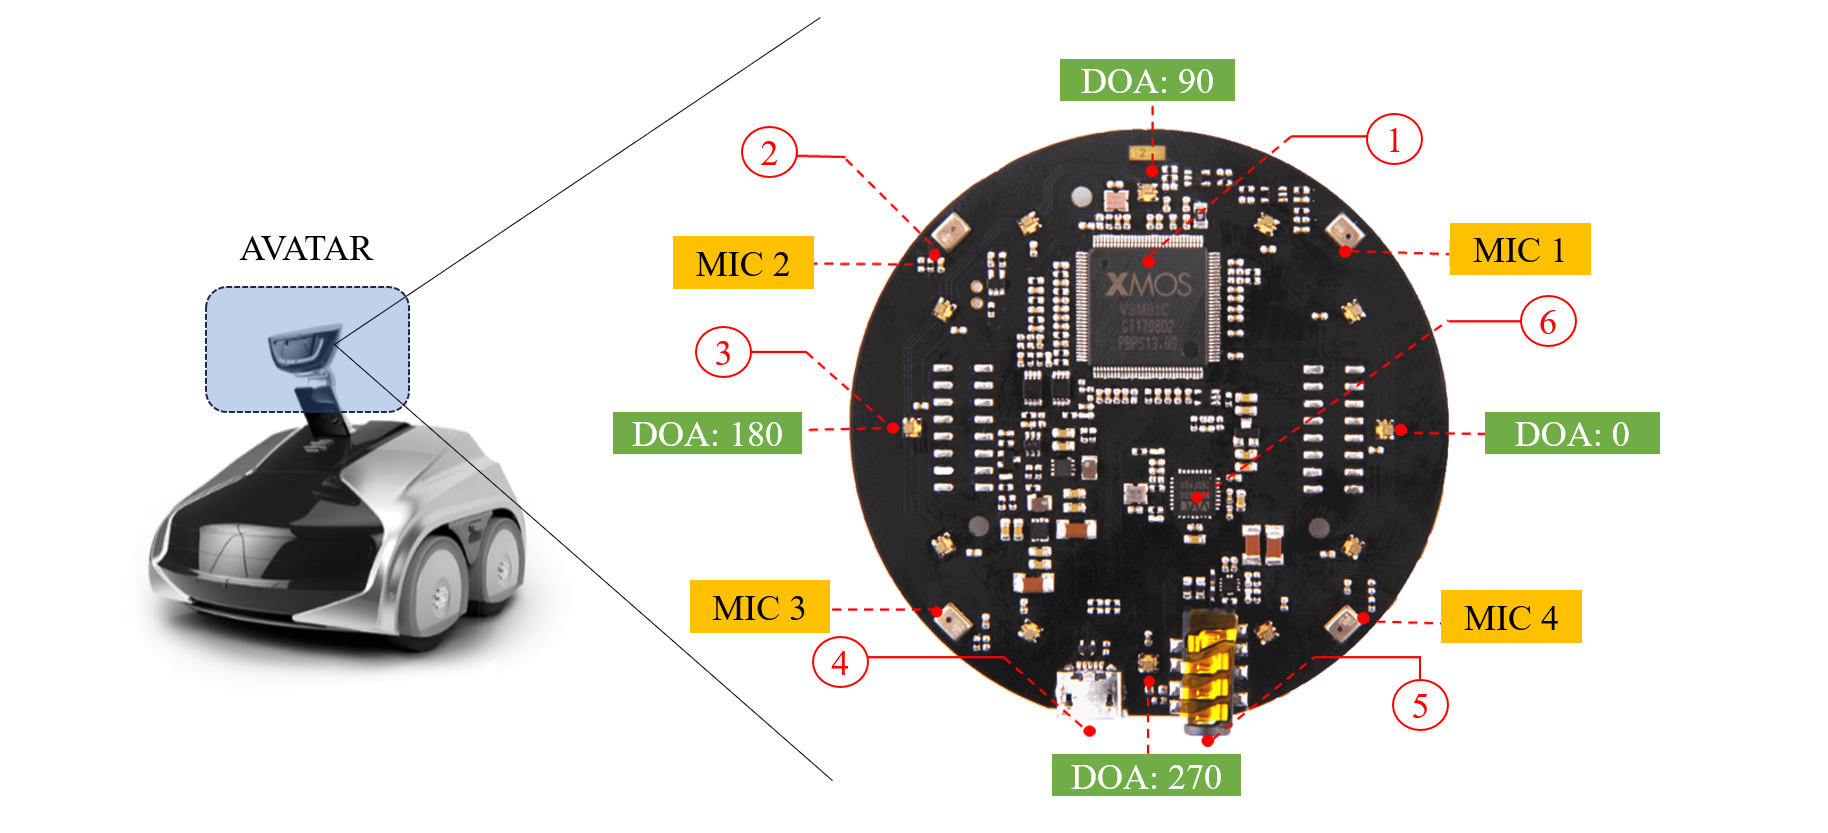
\includegraphics[width=.85\textwidth]{resources/images/050-methods/Methods_evaluation_microphone_ReSpeaker_Mic_Array_v2.0.png}
        \smallcaption{Source: Author, "adapted from" \textcite{ReSpeake72} }
        \label{fig:methods_evaluation_AVATAR_ReSpeaker}
\end{figure}

As described in subsection \ref{subsec:objectives_general}, the C-Bot hardware is not available in Brazil for testing therefore, the best-performing model was deployed in a high-end general-purpose platform identical to the AVATAR, namely Raspberry Pi 4 model B \cite{Raspberry2023}, hereinafter named only as Raspberry Pi, with 8 \gls{g}\gls{b} SDRAM and Quad core Cortex-A72 (ARM v8) 64-bit SoC @1.8 \gls{g}\gls{hz}. 

Before the evaluation flow took place in the VW UP, an experiment was performed indoor to evaluate the soundness of the predictive algorithm. This experimental setup involved connecting a single microphone directly to a Raspberry Pi to facilitate live prediction with an interval of 1 \gls{s}. The Raspberry Pi housed both the audio clips employed by the algorithm and the vectors for prediction results, alongside recording the total prediction time. Concurrently, an identical microphone was connected to a notebook to record audio continuously. Both recordings were initiated simultaneously to ensure temporal alignment as illustrated by Figure \ref{fig:methods_evaluation_indoor_experiment}.

\begin{figure}[htbp]
    \raggedright
        \caption{Setup of the indoor experiment using the Raspberry Pi and the notebook.}
        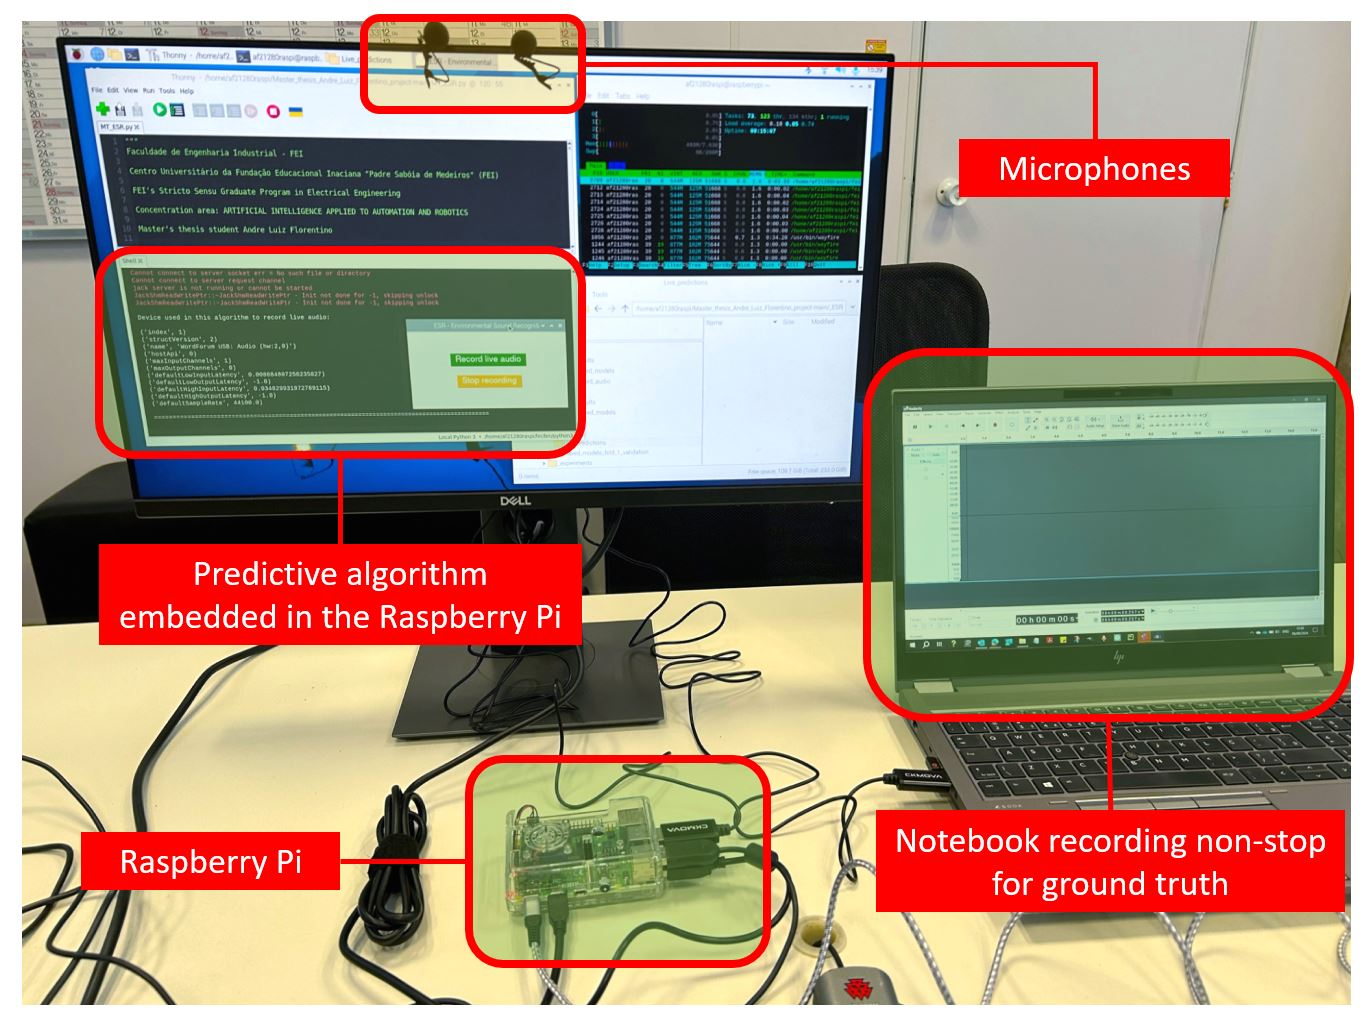
\includegraphics[width=.8\textwidth]{resources/images/050-methods/Methods_evaluation_indoor.jpg}
        \smallcaption{Source: Author}
        \label{fig:methods_evaluation_indoor_experiment}
\end{figure}

The sound source, emanating from an iPhone 11 positioned 5 meters away from the microphones, had a duration of 120 \gls{s}. For the creation of ground truth labels, the continuous audio recorded on the notebook was processed using the software Audacity \cite{Audacity2024}. Initial labels were generated according to the evaluated class, segmented into equal intervals of 1 \gls{s} each. Silence periods were automatically identified within a range of -20 \gls{db} to -30 \gls{db}, contingent upon the class under evaluation. Subsequently, these labels underwent manual adjustment through auditory inspection, ensuring accuracy by comparing the labeled segments with identified silence periods (Fig. \ref{fig:methods_evaluation_audacity_ground_truth}).

This approach ensured that the ground truth labels were precisely aligned with the actual audio events, thereby providing a reliable benchmark for evaluating the performance of the predictive algorithm in real-time conditions.

\begin{figure}[htbp]
    \raggedright
        \caption{Creation of the ground truth labels using software Audacity.}
        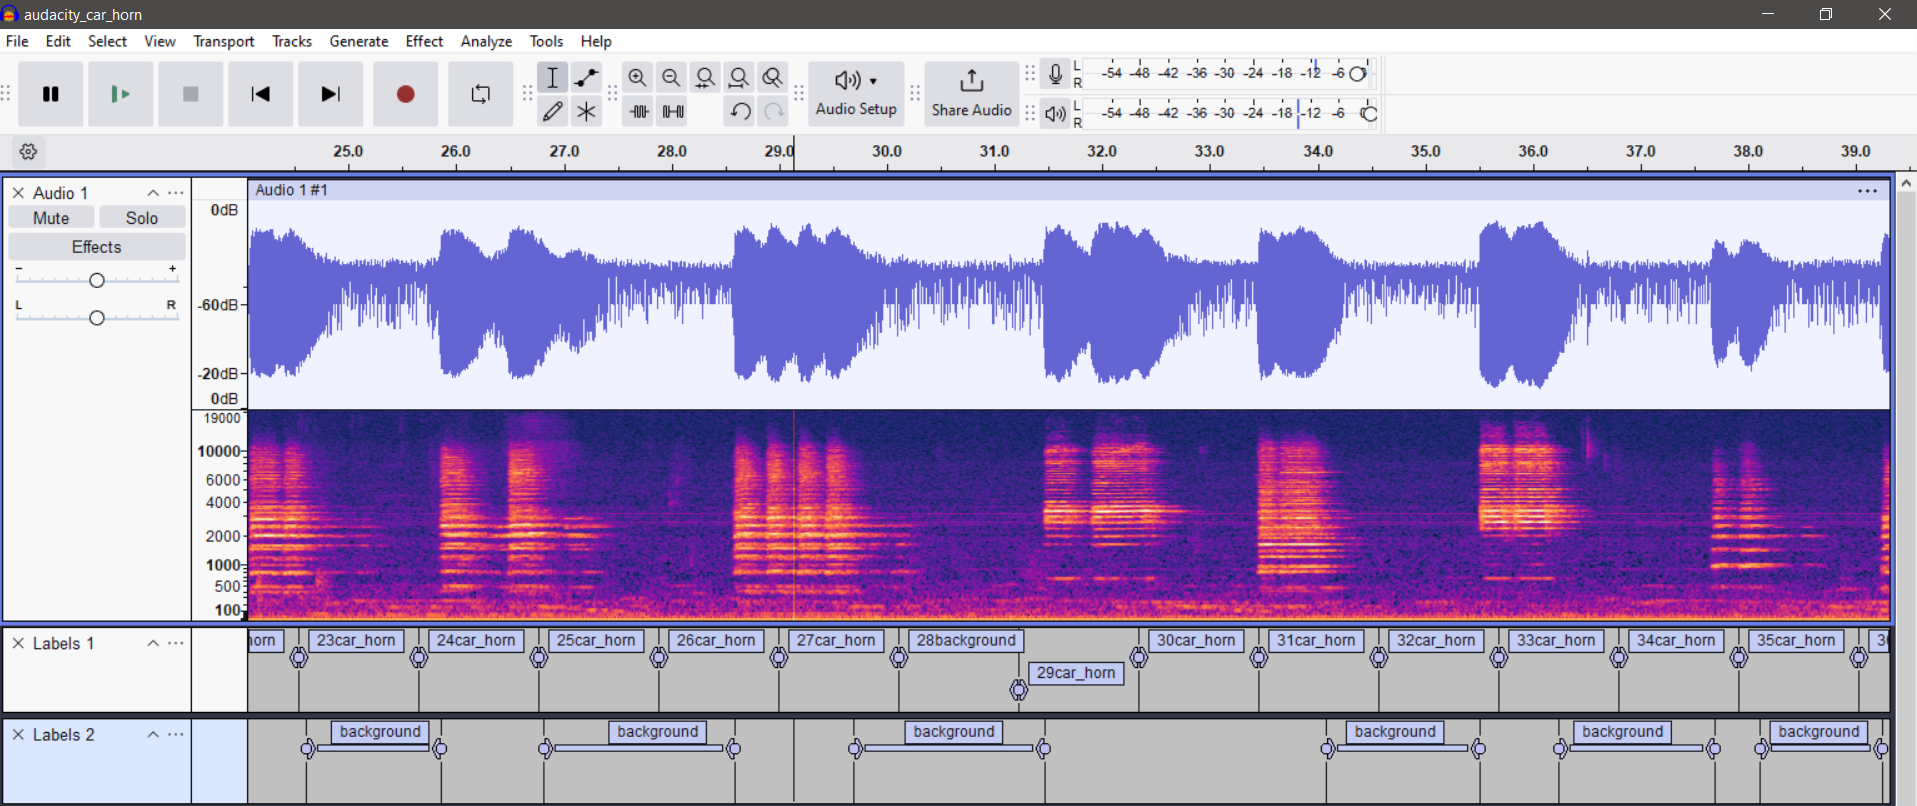
\includegraphics[width=1\textwidth]{resources/images/050-methods/Methods_evaluation_audacity_ground_truth.png}
        \smallcaption{Source: Author}
        \label{fig:methods_evaluation_audacity_ground_truth}
\end{figure}

The evaluation flow was conducted inside of the VW UP, however, the installed microphone illustrated by Figure \ref{fig:methods_evaluation_microphone_aftersales_and_VW_UP} (b) manufactured by the company BURY, with hypercardioid characteristics, electret type, output level Ua (Meß) of 67 mVeff $\pm$3 \gls{db}, acoustic pressure pMeß of 0.1 Pa, and frequency response not informed \cite{BURY2024} was replaced by a lapel microphone model USB Lavalier LUM2 series, condenser type, omnidirectional, with frequency response of 50 Hz to 20 kHz, signal-to-noise ratio 50 dB SPL, and sensitivity of -34 dB ±3 dB \cite{CKMOVA2021} as depicted in Figure \ref{fig:methods_evaluation_microphone_aftersales_and_VW_UP} (a).

The approach employed in the indoor experiments was similarly applied to the outdoor experiments (Figure \ref{fig:methods_evaluation_outdoor_experiment}), however, due to the direct connection between the Raspberry Pi and the notebook via the USB-C port and the additional latency introduced into the system through this connection, the total prediction time for these experiments was excluded from consideration. Moreover, it was not possible to start both applications simultaneously (live prediction in the Raspberry Pi and continuously audio for the ground truth in the notebook), and therefore, a starting and ending flag were establishing using voice command to manually synchronize the audios afterwards in the software Audacity.

\begin{figure}[htbp]
    \raggedright
        \caption{Microphone utilized in the experiments.}
        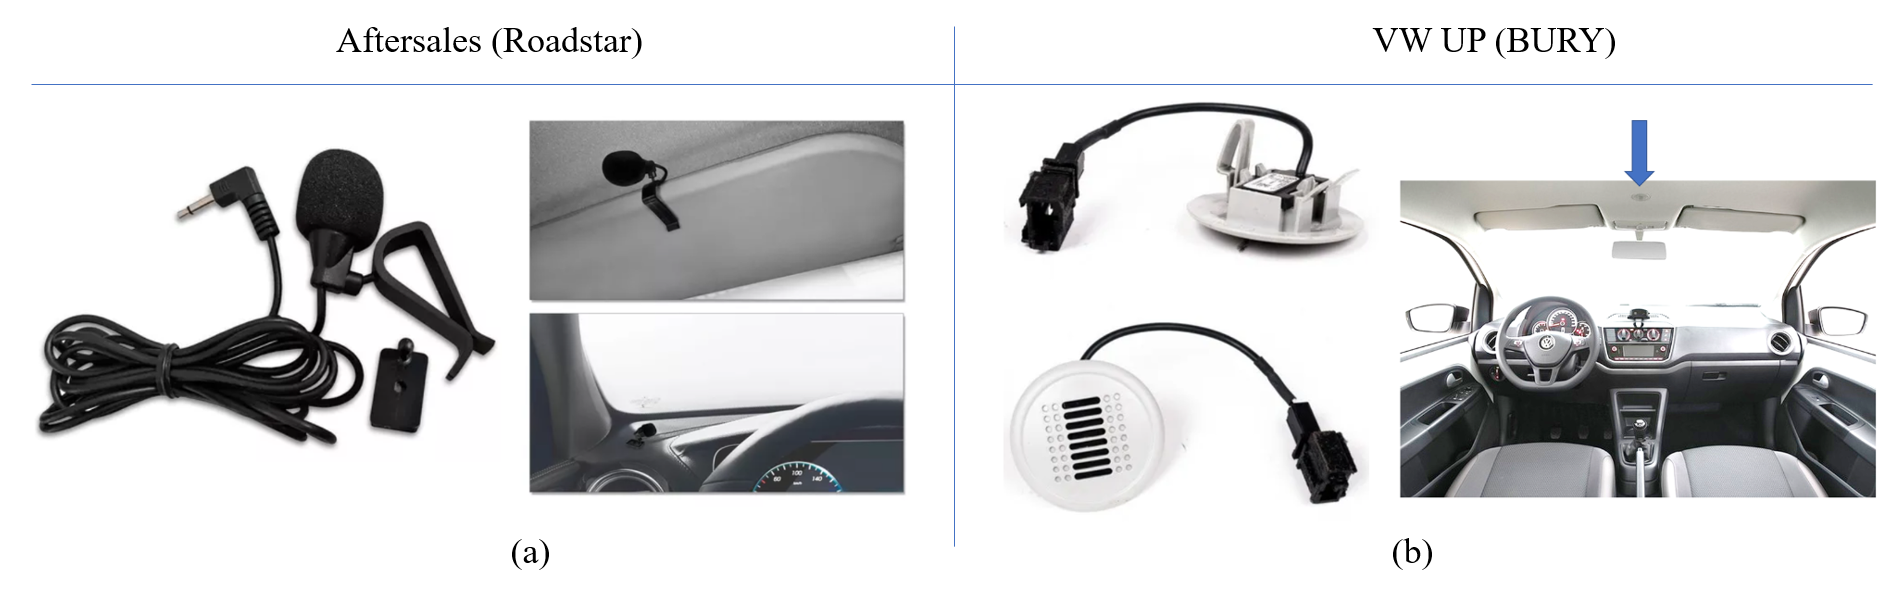
\includegraphics[width=1\textwidth]{resources/images/050-methods/Methods_evaluation_microphone_aftersales_VW_UP.png}
        \smallcaption{Source: Author, "adapted from" \textcite{Roadstar2021} and \textcite{BURY2024} }
        \label{fig:methods_evaluation_microphone_aftersales_and_VW_UP}
\end{figure}

\begin{figure}[htbp]
    \raggedright
        \caption{Setup of the outdoor experiment using the Raspberry Pi and the notebook.}
        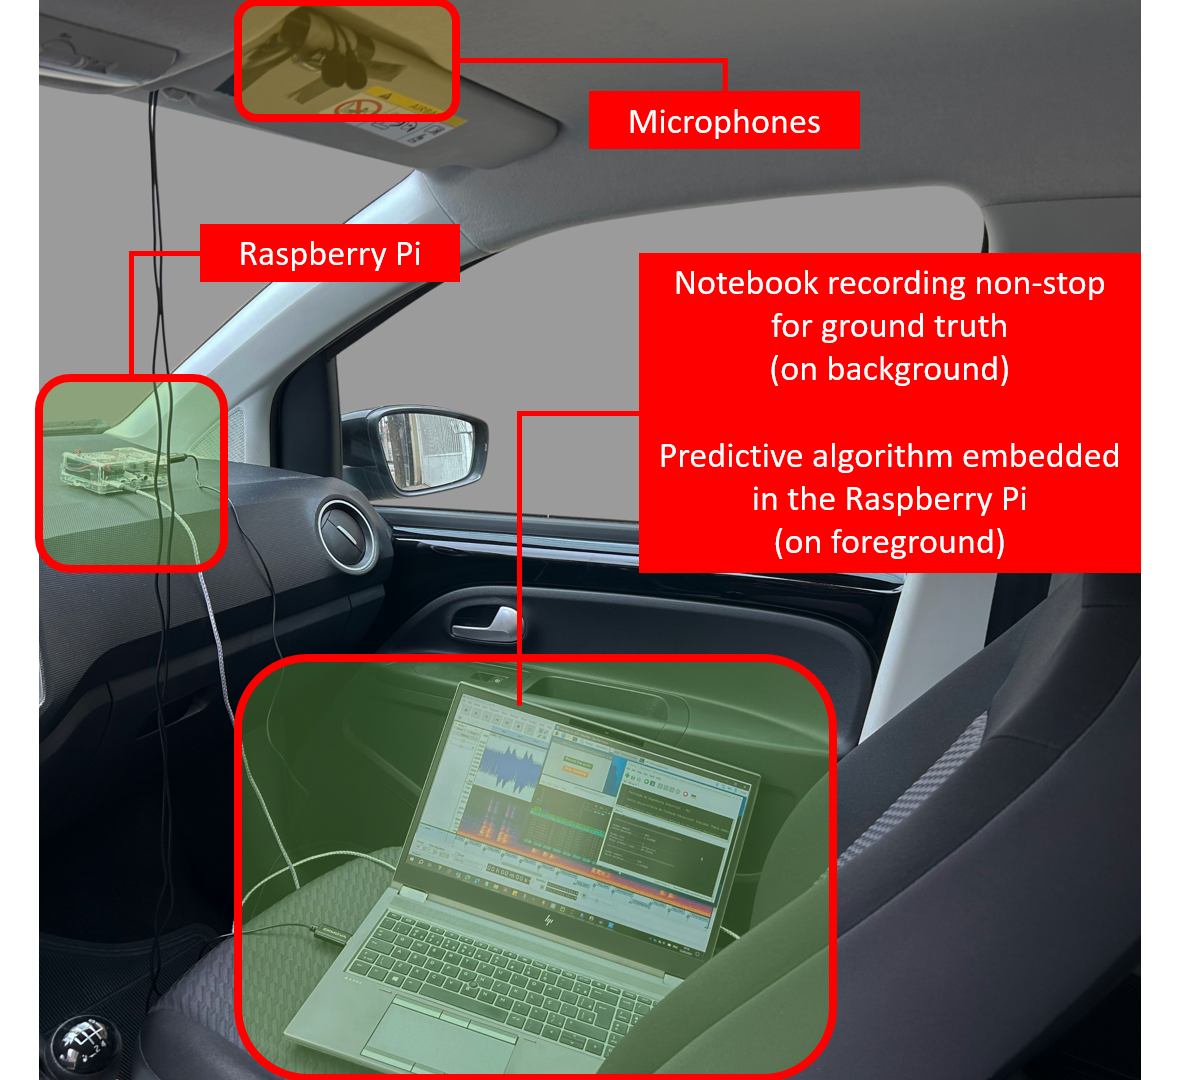
\includegraphics[width=.8\textwidth]{resources/images/050-methods/Methods_evaluation_outdoor.png}
        \smallcaption{Source: Author}
        \label{fig:methods_evaluation_outdoor_experiment}
\end{figure}
\chapter{RESULTS}
\label{chp:results}

In addition to employing grid search and built-in cross-validation to optimize the classifiers described in Chapter \ref{chp:methods}, the impact of two methods to rescale the features was evaluated: normalization and standardization. Furthermore, the influence of \gls{pca} by considering 98\% of the explained variance was also investigated, resulting in approximately 50\% reduction in the number of features. All analysis and results henceforth were evaluated in Excel, with examples using the ESC-10 dataset depicted in Figures \ref{fig:results_ESC-10_classification_results_overview} and \ref{fig:results_ESC-10_classification_results_fold_overview}. The results were compiled in the subsequent sections only as tables.

\begin{figure}[htbp]
    \centering
        \caption{Overview of the results of the classifiers during the training / classification flow - Example with the ESC-10 dataset.}
        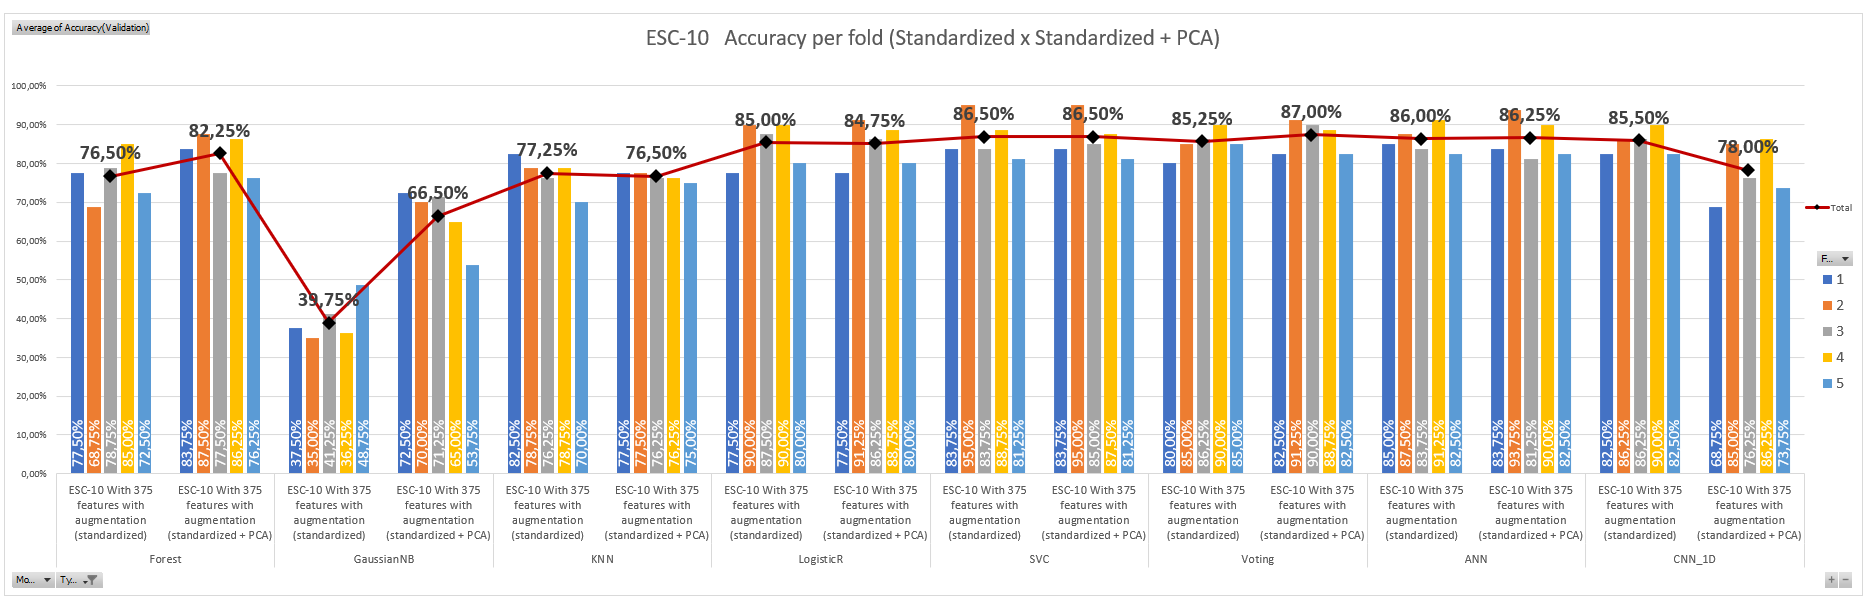
\includegraphics[width=1\textwidth]{resources/images/060-results/Results_classification_flow_ESC-10_2.png}
        \smallcaption{Source: Author}
        \label{fig:results_ESC-10_classification_results_overview}
\end{figure}

\begin{figure}[htbp]
    \centering
        \caption{Comparison of the best option for the classifiers results per fold during the training / classification flow - Example with the ESC-10 dataset features original x features augmented.}
        \includegraphics[width=.95\textwidth]{resources/images/060-results/Results_classification_flow_ESC-10_1.png}
        \smallcaption{Source: Author}
        \label{fig:results_ESC-10_classification_results_fold_overview}
\end{figure}


\section{BENCHMARK}
\label{sec:results_metrics}

% Specific objective a) 

This section presents the basic benchmark metrics gathered within the body of literature (Chapter \ref{chp:rel}). Starting with human accuracy, according to \textcite{PiczakESC2015}, an average accuracy rate of 95.7\% was attained for the ESC-10 dataset, while the ESC-50 dataset achieved an accuracy rate of 81.3\%. The recall rates for individual sound event classes displayed significant variation, ranging from 34.1\% for washing machine noise to nearly 100\% for crying babies and barking dogs. These experiments indicate that proficient and attentive listeners have the potential to achieve perfect scores on the smaller dataset and are likely to reach accuracy levels of approximately 90\% on the main dataset, albeit with some uncertainties when categorizing more ambiguous mechanical noises and soundscapes.

To ensure the soundness of the \gls{esr} algorithm, accuracy rates of benchmark datasets were initially compiled from the literature, but only the ones that fully comply with the dataset specifications, more specifically, with k-fold cross-validation setting of 5 for ESC-10, 3 for BDLib2 and 10 for \gls{us8k}. Thus, the values were collected from \textcite{PiczakESC2015}, \textcite{Bountourakis2019}\footnote{The \gls{sti} method better matches the features utilized in this study, with 75.2\% \gls{ann}, 75.0\% \gls{glm}, and 73.6\% \gls{lr}, nevertheless, the highest results were considered in the table.} with the \gls{eti} method,  \textcite{Salamon2014}, and \textcite{Vandendriessche2021} in Table \ref{table:results_benchmark_accuracy}.

\begin{table}[ht!]
    \caption[Accuracy results benchmark of the datasets]{Compilation of the accuracy results to establish a benchmark on the utilized datasets.}
    \label{table:results_benchmark_accuracy}
    \centering
    \begin{tabular}{
        >{\raggedright\arraybackslash}m{0.28\textwidth} | >
        {\centering\arraybackslash}m{0.20\textwidth} | >
        {\centering\arraybackslash}m{0.20\textwidth} | >
        {\centering\arraybackslash}m{0.20\textwidth}}
        \Xhline{2\arrayrulewidth}
        \rowcolor{lightgray}
        \textbf{Classifier} & \textbf{ESC-10} & \textbf{BDLib2} & \textbf{\gls{us8k}}\\
        \hline
        \gls{k-nn}    & 66.7\% & ---    & 56.0\%  \\
        \gls{gnb}     & ---    & ---    & ---     \\
        \gls{svm}     & 67.0\% & ---    & 69.0\%  \\
        \gls{lr}      & ---    & 74.8\% & ---     \\
        \gls{rf}      & 72.7\% & ---    & 66.0\%  \\
        Voting        & ---    & ---    & 10.0\%  \\
        \gls{glm}     & ---    & 80.4\% & ---     \\
        Decision tree & ---    & ---    & 48.0\%  \\
        \gls{ann}     & ---    & 81.5\% & ---     \\
        \gls{cnn} 1D  & 83.2\% & ---    & 60.1\%  \\
     \Xhline{2\arrayrulewidth}
    \end{tabular}
    \smallcaption{Source: Author}
\end{table}

\section{TRAINING AND CLASSIFICATION FLOW}
\label{sec:results_training_classification_flow}

In this initial stage of the experiments, the main objective is to evaluate the \gls{esr} algorithm implemented with several classifiers regarding its feature selection, feature extraction, classification metrics, processing memory, flash memory, and response time. The evaluation was performed both in a notebook and embedded in the Raspberry Pi 4.

To evaluate the feature selection, a Python script was developed to generate various models for k-fold cross-validation. These models included normalization, standardization, normalization + \gls{pca}, and standardization + \gls{pca}. Each model was applied to both the original and augmented datasets. On average, the accuracy rates of the top-performing classifiers increased among the datasets ESC-10 (1.5\%) and BDLib2 (7.4\%) but decreased in the \gls{us8k} (-0.7\%). Notably, as depicted in Table \ref{table:results_accuracy_overview_classifiers_aug_ori_1}, the winning classifiers were mostly the models \textbf{augmented normalized} and \textbf{augmented standardized} for ESC-10 and BDLib2, while for \gls{us8k} were the models \textbf{original normalized} and \textbf{original standardized}. The differences between the exceptions and these models were marginal.

\begin{table}[ht!]
    \caption[Accuracy rates overview using the benchmark datasets - Models augmented x original (Focus on the classifiers line by line)]{Accuracy rates overview using the benchmark datasets - The color gradient focuses on the classifiers utilized in the models augmented and original, line by line.}
    \label{table:results_accuracy_overview_classifiers_aug_ori_1}
     \raggedright
    \includegraphics[width=1\textwidth]{resources/images/060-results/Results_classification_overview_aug_x_ori_1.png}
    \smallcaption{Source: Author}
\end{table}

When analyzing the entire datasets with their respective classifiers, notable performance for the ESC-10 and BDLib2 datasets was observed among classical machine learning techniques, with \textbf{\gls{lr}} and \textbf{\gls{svm}} emerging as the top performers along with the ensemble method \textbf{\gls{rf}}. This pattern was not identified in the \gls{us8k}, where the neural networks performed better in every model, more specifically, in the normalized and standardized models. Consistently, the same behavior from classifier by classifier emerged in the dataset by dataset, wherein models \textbf{augmented} for ESC-10 and BDLib2 and \textbf{original} for \gls{us8k} yielded the best results, as illustrated by the color gradient in Table \ref{table:results_accuracy_overview_classifiers_aug_ori_2}. 

\begin{table}[ht!]
    \caption[Accuracy rates overview using the benchmark datasets - Models augmented x original (Focus on the classifiers dataset by dataset)]{Accuracy rates overview using the benchmark datasets - The color gradient is focused on the classifiers utilized in the models augmented and original, dataset by dataset.}
    \label{table:results_accuracy_overview_classifiers_aug_ori_2}
     \raggedright
    \includegraphics[width=1\textwidth]{resources/images/060-results/Results_classification_overview_aug_x_ori_2.png}
    \smallcaption{Source: Author}
\end{table}

The feature extraction process was evaluated following two methods: the first employed a sliding window of 1 \gls{s}, a sampling rate of 22,050 \gls{hz}, and 50\% overlapping, while the second method utilized the entire audio file (single window) as input also with a sampling rate of 22,050 \gls{hz}. In the first method (windowed), the accuracy across all datasets exhibited an approximate 5\% decline, as evidenced by the gradient color variations among the classifiers presented in Table \ref{table:results_accuracy_overview_features_windowed}. This result aligns well with the findings from \textcite{Salamon2014}, wherein both classifiers \gls{svm} and \gls{rf} also had a decrease in accuracy of around 5\% (graphically estimated) when transitioning from 4 \gls{s} to 1 \gls{s} audio slices. 

\begin{table}[ht!]
    \caption[Accuracy rates overview using the benchmark datasets - Models augmented x windowed (Focus on the classifiers dataset by dataset)]{Accuracy rates overview using the benchmark datasets - The color gradient focuses on the classifiers utilized in the models augmented and windowed, dataset by dataset.}
    \label{table:results_accuracy_overview_features_windowed}
     \raggedright
    \includegraphics[width=1\textwidth]{resources/images/060-results/Results_classification_overview_aug_x_ori_3.png}
    \smallcaption{Source: Author}
\end{table}

At this point, the benchmark Table \ref{table:results_benchmark_accuracy} was updated with the best accuracy results from Table \ref{table:results_accuracy_overview_classifiers_aug_ori_2}. The comparison is presented in Table \ref{table:results_accuracy_comparison}, and it entails that the feature selection was sound overcoming all results of comparable classifiers except by the \gls{ann} in the BDLib2 dataset.

\begin{table}[ht!]
    \caption[Comparison of the accuracy results benchmark with the best models from cross-validation]{Compilation of the benchmark (BM) results against the augmented normalized models for ESC-10 and BDLib2 and original normalized models for \gls{us8k}.}
    \label{table:results_accuracy_comparison}
    \centering
    \begin{tabular}{
        >{\raggedright\arraybackslash}m{0.15\textwidth} | >
        {\centering\arraybackslash}m{0.10\textwidth} | >
        {\columncolor{lime}\centering\arraybackslash}m{0.12\textwidth} | >
        {\centering\arraybackslash}m{0.10\textwidth} | >
        {\columncolor{lime}\centering\arraybackslash}m{0.12\textwidth} | >
        {\centering\arraybackslash}m{0.10\textwidth} | >       
        {\columncolor{lime}\centering\arraybackslash}m{0.11\textwidth}}
        \Xhline{2\arrayrulewidth}
        \rowcolor{lightgray}
        \textbf{Classifier} & \textbf{ESC-10} & \textbf{ESC-10} & \textbf{BDLib2} & \textbf{BDLib2} & \textbf{US8K} & \textbf{US8K} \\
        \rowcolor{lightgray}
        & BM & Aug. norm & BM & Aug. norm & BM & Ori. norm \\
        \hline
        k-NN            & 66.7\% & 76.3\% & ---    & 69.3\% & 56.0\% & 57.2\%   \\
        GNB             & ---    & 72.9\% & ---    & 66.5\% & ---    & 45.1\%   \\
        SVM             & 67.0\% & 87.9\% & ---    & 77.4\% & 69.0\% & 70.4\%   \\
        LR              & ---    & 86.8\% & 74.8\% & 78.1\% & ---    & 69.6\%   \\
        RF              & 72.7\% & 86.7\% & ---    & 81.0\% & 66.0\% & 68.1\%   \\
        Voting          & ---    & 86.4\% & ---    & 76.7\% & 10.0\% & 71.5\%   \\
        GLM             & ---    & ---    & 80.4\% & ---    & ---    & ---      \\
        Decision tree   & ---    & ---    & ---    & ---    & 48.0\% & ---      \\
        ANN             & ---    & 86.2\% & \cellcolor{lime}81.5\% & \cellcolor{white} 78.1\% & --- & 71.5\%   \\
        CNN 1D          & 83.2\% & 85.7\% & ---    & 78.6\% & 60.1\% & 72.0\%   \\          
    \Xhline{2\arrayrulewidth}
    \end{tabular}
    \smallcaption{Source: Author}
\end{table}


% Specific objective b).

The dataset created in subsection \ref{subsec:dataset_US8K_AV}, referred to as US8K\_AV, consists of 4,908 files distributed across 6 classes. These files collectively represent a total duration of 4.94 hours of recorded sounds. To maintain consistency and facilitate accuracy comparisons, the original 10-fold split for cross-validation from the source dataset (\gls{us8k}) was retained.

Similarly to the \gls{us8k} dataset, the augmentation process resulted in a slight decline in accuracy rates for the top-performing classifiers among the machine learning techniques, whereas the neural network models exhibited a marginal improvement (Table \ref{table:results_accuracy_overview_us8k_av_aug_ori_1}, upper area). Given the time-consuming effort required for training the augmented model and the substantial increase in the size of the feature model subsequently, there appears to be no practical justification for adopting augmentation techniques within this tailored dataset.

Considering the original normalized model, \textbf{\gls{svm}} and \textbf{\gls{ann}} outperformed the other classifiers, achieving an average accuracy of 83\%. These were followed by \textbf{\gls{lr}} and \textbf{\gls{cnn} 1D}, both attaining an accuracy of 82\%. Notably, \gls{ann} demonstrated the highest stability among the models, with its accuracy consistently ranging between 82\% and 83\%. A comparable pattern emerged in the windowed normalized models (Table \ref{table:results_accuracy_overview_us8k_av_aug_ori_1}, lower area), with the same four classifiers ranked as top performers. However, the sliding window process introduced the same overhead noticed in the other datasets, reducing the average accuracy by 5\%, ranging now between 77\% and 79\%.

\begin{table}[ht!]
    \caption[Accuracy rates overview using the tailored dataset US8K\_AV.]{Accuracy rates overview of the best models using the tailored dataset US8K\_AV.}
    \label{table:results_accuracy_overview_us8k_av_aug_ori_1}
     \raggedright
    \includegraphics[width=1\textwidth]{resources/images/060-results/Results_classification_overview_us8k_av_aug_x_ori_1.png}
    \smallcaption{Source: Author}
\end{table}

%The $t$\_statistic` specifically quantifies the difference between the means of these two groups, normalized by the variability of their differences. It serves as an indicator of whether there is a statistically significant difference between the two sets of accuracy measurements. A higher absolute value of $t$\_statistic suggests a greater likelihood that the observed difference is not due to random chance.

To finalize the evaluation of the feature extraction process, the aforementioned 5\% reduction in accuracy between the augmented and windowed models was statistically evaluated with paired samples $t$-test using the results plotted in Table \ref{table:results_accuracy_overview_features_windowed} and Table \ref{table:results_accuracy_overview_us8k_av_aug_ori_1}. The hypotheses for this evaluation were formulated as follows:

\begin{itemize}
    \item Null hypothesis ($H_0$): There is no significant difference between the performance of the augmented model and the windowed model;
    \item Alternative hypothesis ($H_a$): There is a significant difference between the performance of the augmented model and the windowed model.
\end{itemize}

Given the $p$-value = 0.005, the null hypothesis was rejected in all datasets, as illustrated in Table \ref{table:results_paired_t-test_datasets}, and therefore, there is a statistically significant difference in performance between the augmented and windowed models within the datasets and classifiers analyzed. This pattern was also observed across classifiers among the datasets, albeit with a higher probability ($p$-value = 0.05) and with \gls{gnb} as the exception (Table \ref{table:results_paired_t-test_classifiers}).

%This result is not conclusive; rather, it provides evidence that needs to be consistently observed and replicated in further studies to identify a reliable trend.

\begin{table}[ht!]
    \caption[Statistic evaluation of the accuracy results between the augmented and windowed models among datasets]{Statistic evaluation of the accuracy results between the augmented and windowed models among datasets.}
    \label{table:results_paired_t-test_datasets}
    \centering
    \begin{tabular}{
        >{\arraybackslash}m{0.30\textwidth} | >
        {\centering\arraybackslash}m{0.30\textwidth} | >
        {\centering\arraybackslash}m{0.30\textwidth}}
        \Xhline{2\arrayrulewidth}
        \rowcolor{lightgray}
        \textbf{Dataset} & \textbf{$t$-test statistic} & \textbf{$p$-value}\\
        \hline
            BDLib2      & 4.064637      & 0.004781 \\
            ESC-10      & 7.491015      & 0.000138 \\
            \gls{us8k}  & 6.106191      & 0.000488 \\
            US8K\_AV    & 4.974953      & 0.001610 \\
     \Xhline{2\arrayrulewidth}
    \end{tabular}
    \smallcaption{Source: Author}
\end{table}


\begin{table}[ht!]
    \caption[Statistic evaluation of the accuracy results between the augmented and windowed models among classifiers]{Statistic evaluation of the accuracy results between the augmented and windowed models among classifiers.}
    \label{table:results_paired_t-test_classifiers}
    \centering
    \begin{tabular}{
        >{\arraybackslash}m{0.30\textwidth} | >
        {\centering\arraybackslash}m{0.30\textwidth} | >
        {\centering\arraybackslash}m{0.30\textwidth}}
        \Xhline{2\arrayrulewidth}
        \rowcolor{lightgray}
        \textbf{Classifier} & \textbf{$t$-test statistic} & \textbf{$p$-value}\\
        \hline
            \gls{rf}     & 8.872540       & 0.003019 \\
            \gls{gnb}    & 1.977806       & 0.142361 \\
            \gls{k-nn}   & 5.265241       & 0.013351 \\
            \gls{lr}     & 3.211662       & 0.048894 \\
            \gls{svm}    & 3.320547       & 0.045036 \\
            Voting       & 3.346427       & 0.044176 \\
            \gls{ann}    & 5.679546       & 0.010816 \\
            \gls{cnn} 1D & 5.378761       & 0.012585 \\
     \Xhline{2\arrayrulewidth}
    \end{tabular}
    \smallcaption{Source: Author}
\end{table}


% Specific objective c).

During the training of the \gls{cnn} 2D models, the architecture that demonstrated the best performance for the sliding window process was adapted from \textcite{Su2020}, achieving an average accuracy of 80\% with 1.5 million trainable parameters. This model also presented a decrease in accuracy between the augmented and windowed models (statistically confirmed across folds with paired sample $t$-test and $p$-value < 0.05). Notably, the model adapted from \textcite{Luz2021} had fewer trainable parameters (200,000) and attained the highest score (86\%) in the single window process. However, it exhibited a significant drop in accuracy during the sliding window process, decreasing to 77\%, as shown in Table \ref{table:results_accuracy_overview_us8k_av_cnn_2D}. This pattern was consistently observed across all datasets, including a modest improvement in average accuracy resulting from the augmentation process, which was not identified in the previous classifiers. Due to resource limitations and low trade-offs, the windowed augmented model was not investigated.

\begin{table}[ht!]
    \caption[Accuracy rates for each fold of the tailored dataset US8K\_AV.]{Accuracy rates for each fold of the tailored dataset US8K\_AV, models original and augmented, both using two different architectures.}
    \label{table:results_accuracy_overview_us8k_av_cnn_2D}
     \raggedright
    \includegraphics[width=1\textwidth]{resources/images/060-results/Results_classification_overview_us8k_av_cnn2d.png}
    \smallcaption{Source: Author}
\end{table}


At this moment, the following outcomes were identified and will henceforth be adopted:
\begin{itemize}
    \item Models utilizing handcrafted features will be normalized. The processes of standardization and \gls{pca} will no longer be considered for these models;
    \item The augmentation process has been observed to enhance the performance of \gls{cnn} 2D models across all datasets, however, it will not be applied in the windowed model for the US8K\_AV dataset;
    \item A comprehensive benchmark has been established for top-performing classifiers using k-fold cross-validation accuracy metrics (Table \ref{table:results_feature_extraction_and_classifiers_us8k_av}). This benchmark includes:
    \begin{itemize}
        \item Machine learning techniques employing handcrafted features: \textbf{\gls{svm}} and \textbf{\gls{lr}};
        \item Neural networks utilizing handcrafted features: \textbf{\gls{ann}} and \textbf{\gls{cnn} 1D};
        \item Neural networks utilizing aggregated features: \textbf{\gls{cnn} 2D}.
    \end{itemize}
    \item \textbf{\gls{rf}} has been incorporated into the benchmark to represent the results involving ensemble methods;
    \item Only \textbf{windowed models} will be considered in order to minimize the inference time.
\end{itemize}


\begin{table}[ht!]
    \caption[Benchmark accuracy results for the dataset US8K\_AV.]{Compilation of the feature extraction processes and top-performing classifiers on the US8K\_AV dataset.}
    \label{table:results_feature_extraction_and_classifiers_us8k_av}
    \centering
    \begin{tabular}{
        >{\arraybackslash}m{0.30\textwidth} | >
        {\centering\arraybackslash}m{0.30\textwidth} | >
        {\centering\arraybackslash}m{0.30\textwidth}}
        \Xhline{2\arrayrulewidth}
        \rowcolor{lightgray}
        \textbf{Features - Classifier} & \textbf{Sliding window (1 s)} & \textbf{Single window (4 s)}\\
        \rowcolor{lightgray}
        \rowcolor{lightgray}
         &  Acc. (Std) & Acc. (Std)   \\
        \hline
        Handcrafted - \gls{svm}    & 78.96\% \hspace{0.5cm} (1.82\%) & 
                                     83.14\% \hspace{0.5cm} (2.21\%)\\
        Handcrafted - \gls{lr}     & 78.87\% \hspace{0.5cm} (1.49\%) & 
                                     82.27\% \hspace{0.5cm} (2.74\%)\\
        Handcrafted - \gls{rf}     & 75.59\% \hspace{0.5cm} (2.72\%) & 
                                     79.94\% \hspace{0.5cm} (2.63\%)\\
        Handcrafted - \gls{ann}    & 77.93\% \hspace{0.5cm} (3.29\%) & 
                                     83.35\% \hspace{0.5cm} (2.91\%)\\
        Handcrafted - \gls{cnn} 1D & 76.69\% \hspace{0.5cm} (3.74\%) & 
                                     82.40\% \hspace{0.5cm} (2.72\%)\\
        Aggregated - \gls{cnn} 2D  & 80.03\% \hspace{0.5cm} (2.71\%) & 
                                     82.78\% \hspace{0.5cm} (3.60\%)\\
     \Xhline{2\arrayrulewidth}
    \end{tabular}
    \smallcaption{Source: Author}
\end{table}

Upon completing the training and classification flow, the next step involves deploying the best-performing classifier to the Raspberry Pi and evaluating its performance in terms of accuracy and real-time processing capabilities. However, before proceeding, several definitions must be established. A 'predictive model' refers to a trained classifier saved as a pickle file (.PKL) for \gls{svm}, \gls{lr}, and \gls{rf} or as an .HDF5 file for neural networks such as \gls{ann}, \gls{cnn} 1D, and \gls{cnn} 2D. The term 'predictive algorithm' or '\gls{esr} algorithm' encompasses the necessary functions to record live audio, extract features, feed them into the predictive model, and return the inference as a single class.

The 'response time' or 'total prediction time' is defined as the aggregate duration of the individual operations involved in the predictive algorithm. The time required for feature extraction denotes the duration necessary to extract features according to the specified method (handcrafted or aggregated). The average time required by the predictive model to perform sound classification using the feature vectors from all frames is referred to as classification time. Therefore, the total prediction time corresponds to the sum of the feature extraction process and the classification time. However, it does not account for the time required to digitize the audio, which will be involved in the 'full prediction time' corresponding to the sum of this digitization time and the total prediction time.

'Processing memory', particularly \gls{ram}, serves as a critical component in the predictive algorithm, facilitating the rapid storage and retrieval of data necessary for real-time audio signal processing involving the initial stages of sound capture, feature extraction, loading the predictive model, and performing the classification tasks.

The predictive models were trained using folds 2 through 10, reserving fold 1 as the testing set. This decision was substantiated by Table \ref{table:results_accuracy_overview_us8k_av_cnn_2D}, which indicated that fold 1 was among the top five folds across all architectural models. Additionally, fold 1 exhibited an accuracy of 80.54\%, closely aligning with the result of the 10-fold cross-validation (80.03\%). The same analysis was performed on the rest of the top-performing classifiers confirming fold 1 as the testing set. Anticipating the necessity to embed the neural network models, the predictive models for \gls{ann}, \gls{cnn} 1D, and \gls{cnn} 2D underwent a quantization process using TensorFlow Lite (TFLite) with standard parameters. Notably, there was no significant decline in accuracy following this process.

To compare the performance of an algorithm on a notebook and a Raspberry Pi, it is essential to ensure that both devices are in good condition and have similar operating systems. The same version of the algorithm and development environment should be used to guarantee equivalent workload conditions as well as monitor the temperature to avoid throttling and execute multiple tests to obtain a reliable average. Consideration must be given to the differences in processor architectures (x86 vs. ARM) and whether the algorithm can effectively utilize multiple cores. Evaluation of scheduling policies, memory management, and potential conflicts of shared resources among cores is also necessary. Given that the objective of this study is not a quantitative comparison \textit{per se} of these devices but rather a qualitative one, all these factors were verified superficially. The averaged results after 10 loops were compiled in Table \ref{table:results_classifiers_performance_us8k_av}.

\begin{table}[ht!]
    \caption[Processing memory (RAM) and total prediction time.]{Processing memory (RAM) and total prediction time. Comparison between the predictive algorithms in the notebook and Raspberry Pi.}
    \label{table:results_classifiers_performance_us8k_av}
    \centering
    \begin{tabular}{
        >{\raggedright\arraybackslash}m{0.16\textwidth} | >
        {\raggedright\arraybackslash}m{0.15\textwidth} | >
        {\raggedright\arraybackslash}m{0.19\textwidth} | >
        {\raggedright\arraybackslash}m{0.15\textwidth} | >       
        {\raggedright\arraybackslash}m{0.20\textwidth}}
        \Xhline{2\arrayrulewidth}
        \rowcolor{lightgray}
        \textbf{Classifier} & \centering\textbf{Notebook} & \centering\textbf{Notebook} & \centering\textbf{Raspberry Pi} & \centering\textbf{Raspberry Pi} \cr
        \rowcolor{lightgray}
         & \gls{ram} \hfill (Std) & Pred. time \textbf{} (Std) & \gls{ram} \hfill (Std) & Pred. time \hfill (Std) \cr
        \rowcolor{lightgray}
        & \centering (MB) & \centering (ms) & \centering (MB) & \centering (ms) \cr
        \hline
        \gls{svm}    & 34.1  \hfill(4.7)  & 223.4 \hfill(11.4) &  32.4  \hfill(8.2)  & 764.4   \hfill(39.6)   \\
        \gls{lr}     & 1.1   \hfill(0.1)  & 220.7 \hfill(11.8) &  0.2   \hfill(0.03) & 749.2   \hfill(14.6)   \\
        \gls{rf}     & 401.1 \hfill(65.4) & 227.2 \hfill(12.9) &  456.0 \hfill(11.3) & 1,020.9 \hfill(31.1)   \\
        \gls{ann}    & 20.6  \hfill(9.2)  & 250.1 \hfill(16.0) &  0.1   \hfill(0.02) & 752.5   \hfill(12.5)   \\
        \gls{cnn} 1D & 7.5   \hfill(0.5)  & 252.1 \hfill(20.0) &  4.1   \hfill(1.9)  & 750.0   \hfill(13.6)   \\
        \gls{cnn} 2D & 11.7  \hfill(0.2)  & 30.2  \hfill(7.2)  &  19.4  \hfill(2.5)  & 47.6    \hfill(22.0)   \\
    \Xhline{2\arrayrulewidth}
    \end{tabular}
    \smallcaption{Source: Author}
\end{table}

Additionally, the non-volatile storage medium that retains data even when the power is turned off (Flash memory) was also evaluated. In this study, the Flash memory represents the size of the predictive models, sorted by size as follows: 19.0 \gls{k}\gls{b} (\gls{lr}), 6,218.0 \gls{k}\gls{b} (\gls{cnn} 1D), 8,928.0 \gls{k}\gls{b} (\gls{ann}), 11,920.0 \gls{k}\gls{b} (\gls{cnn} 2D), 32,761.0 \gls{k}\gls{b} (\gls{svm}) and 249,522.0 \gls{k}\gls{b} (\gls{rf}). This information was normalized (min -1\% and max +1\% to avoid zero in the log axis) with the values of RAM and total prediction time to create the spider web chart depicted in Figure \ref{fig:Results_spider_chart_us8k_av_cnn2d}, which supports the decision of the predictive algorithm with \textbf{\gls{cnn} 2D} embedded in the Raspberry Pi.

\begin{figure}[htbp]
    \raggedright
        \caption{Spider web chart of the predictive algorithms.}
        \includegraphics[width=1\textwidth]{resources/images/060-results/Results_spider_chart_us8k_av_cnn2d.png}
        \smallcaption{Source: Author}
        \label{fig:Results_spider_chart_us8k_av_cnn2d}
\end{figure}

Prior to the evaluation flow, an indoor experiment, as described in section \ref{sec:methods_evaluation}, was conducted to assess the effectiveness of the predictive algorithm \gls{cnn} 2D. The experimental setup comprised a notebook, a Raspberry Pi, and identical microphones arranged in a meeting room with an average background noise level of 60 \gls{db}, primarily due to air conditioning. The sound source was positioned 5 meters away from the microphones and approximately 120 \gls{s} of audio from YouTube was played at maximum volume on an iPhone 11, resulting in the generation of 107 audio samples. The \gls{spl} measured at the microphones reached a peak of 75 \gls{db} during playback but predominantly ranged between 60 \gls{db} and 65 \gls{db} due to the blending with background noise. The result of this experiment is presented in Table \ref{table:results_indoor_experiments} and inferred a sound algorithm with high precision and f1-score ranging from 77\% to 95\%, both per analyzed class. 

\begin{table}[ht!]
    \caption[Classification metrics of the indoor experiments.]{Classification metrics of the indoor experiments.}
    \label{table:results_indoor_experiments}
    \centering
    \begin{tabular}{
        >{\raggedright\arraybackslash}m{0.26\textwidth} | >
        {\centering\arraybackslash}m{0.15\textwidth} | >
        {\centering\arraybackslash}m{0.15\textwidth} | >
        {\centering\arraybackslash}m{0.15\textwidth} | >
        {\centering\arraybackslash}m{0.15\textwidth}}
        \Xhline{2\arrayrulewidth}
        \rowcolor{lightgray}
        \textbf{Classes} & \textbf{Precision} & \textbf{Recall} & \textbf{F1-score} & \textbf{Samples} \\
        \hline
        \rowcolor{gray!20}
        Played: \hfill dog\_bark & & & & \\
        background        & 60.0\%  & 86.0\%  & 71.0\%  & 14  \\
        children playing  & 0.0\%   & 0.0\%   & 0.0\%   & 0   \\
        dog\_bark         & 97.0\%  & 65.0\%  & 77.0\%  & 93  \\
        \hline
        Weighted avg      & 92.0\%  & 67.0\%  & 77.0\%  & 107 \\
        \hline
        \rowcolor{gray!20}
        Played: \hfill children\_playing & & & & \\
        background        & 0.0\%    & 0.0\%   & 0.0\%   & 0   \\
        car\_horn         & 0.0\%    & 0.0\%   & 0.0\%   & 0   \\
        children playing  & 100.0\%  & 86.0\%  & 92.0\%  & 107 \\
        \hline
        Weighted avg      & 100.0\%  & 86.0\%  & 92.0\%  & 107 \\
        \hline
        \rowcolor{gray!20}
        Played: \hfill car\_horn & & & & \\
        background        & 44.0\%   & 100.0\%  & 61.0\%  & 7   \\
        car\_horn         & 100.0\%  & 84.0\%   & 91.0\%  & 100 \\
        children playing  & 0.0\%    & 0.0\%    & 0.0\%   & 0   \\
        siren             & 0.0\%    & 0.0\%    & 0.0\%   & 0   \\
        \hline
        Weighted avg      & 96.0\%   & 85.0\%   & 89.0\%  & 107 \\
        \hline
        \rowcolor{gray!20}
        Played: \hfill siren & & & & \\
        background        & 67.0\%   & 100.0\%  & 80.0\%  & 2    \\
        children playing  & 0.0\%    & 0.0\%    & 0.0\%   & 0    \\
        dog\_bark         & 0.0\%    & 0.0\%    & 0.0\%   & 0    \\
        siren             & 100.0\%  & 90.0\%   & 95.0\%  & 105  \\
        \hline
        Weighted avg      & 99.0\%   & 91.0\%   & 95.0\%  & 107  \\
        \hline
     \Xhline{2\arrayrulewidth}
    \end{tabular}
    \smallcaption{Source: Author}
\end{table}


\section{EVALUATION FLOW}
\label{sec:results_evaluation_flow}

The evaluation process was conducted on the streets of Santo André and São Bernardo do Campo during regular traffic hours. All vehicle windows were closed, the infotainment system was turned off (no music), there was no additional passenger inside the vehicle (no speech), and the air conditioning was set to level 2, producing an \gls{spl} near the microphones of approximately 65 \gls{db}. Both microphones were attached to the passenger sun visor near the vehicle's Bluetooth microphone.

The first experiment, designated "Driving on streets 01", aimed to evaluate the performance of the \gls{esr} algorithm under real driving conditions, with speeds ranging from 10 to 50 km/h and maximum \gls{spl} of 80 \gls{db}. This setting involved a broad soundscape typically encountered in large cities. The experiment lasted 3,690 \gls{s} ($\approx$1 hour) and produced 3,310 audio clips, each lasting approximately 1.114578 \gls{s} instead of the intended 1 \gls{s}. This discrepancy was caused by the chunk size of 8,192 samples used in the Raspberry Pi to prevent overflow during audio recording. 

Although none of the relevant classes (dog\_bark, children\_playing, car\_horn, and siren) were present during the experiment, the results demonstrated a robust algorithm with an F1-score reaching 99\%, as illustrated by the confusion matrix in Figure \ref{fig:Results_evaluation_driving_streets_01}.

\begin{figure}[htbp]
    \raggedright
        \caption{Confusion matrix of the first experiment, "Driving on streets 01" without the presence of relevant classes.}
        \includegraphics[width=.65\textwidth]{resources/images/060-results/Results_evaluation_driving_streets_01.png}
        \smallcaption{Source: Author}
        \label{fig:Results_evaluation_driving_streets_01}
\end{figure}

The chunk function in Python operates as a buffer, with each buffer containing 1,024 samples by default, which can then either be retained or discarded by the algorithm. If recorded and saved without segmentation, continuous data flow from a microphone would excessively consume processor resources and potentially lead to system crashes. To address this issue, most Python libraries utilize chunks of data instead of a continuous audio stream. While in the notebook, the chunk size can be set to lower values such as 256 or 512 without overflow problems, in the context of Raspberry Pi, where resources are limited, chunking the data with higher values (2,048, 4,096 or higher) facilitates smoother stream flow and prevents memory leaks. However, higher chunk sizes introduce some latency in the audio recording, on average a few dozen \gls{mi}\gls{s}, reaching no more than one hundred \gls{mi}\gls{s} at higher values.

In an effort to mitigate the latency induced by the chunk size of 8,192 samples employed in the \gls{esr} algorithm embedded in the Raspberry Pi, three experiments were conducted with the chunk size adjusted to 4,096, representing the upper limit before encountering buffer input overflow. For reference, the chunk size utilized in the notebook was set to 1,024 samples. 

The first experiment, titled "Driving on Streets 02", with one class of interest (siren), spanned a duration of 737 \gls{s} and resulted in the generation of 721 audio clips. The second experiment, "Driving on Streets 03", also with one class of interest (dog\_bark), had a considerably longer duration of 2,834 \gls{s} and produced 2,774 audio clips. The final experiment, "Driving on Streets 04", with two classes of interest (siren and car\_horn), lasted for 1,368 \gls{s} and yielded 1,339 audio clips. Each of these experiments produced audio clips with approximately 1.021678 \gls{s} instead of 1.114578 \gls{s}, nevertheless, the F1-score in all three experiments was considerably lower, reaching 50\%, 22\% and 50\% respectively.

By comparing the audio clip recorded in the Raspberry Pi with the corresponding segment from the continuous audio recorded in the notebook, it is evident that the reduction in chunk size induced distortions across various frequency bands, as illustrated in Figure \ref{fig:Results_evaluation_driving_streets_02_04}, and adversely affected the inferences generated by the predictive algorithm. These distortions were also subjectively confirmed by manually listening and comparing the audio clips.

\begin{figure}[htbp]
    \raggedright
        \caption{Comparison between the audio clip recorded with chunk = 4,096 in the Raspberry Pi and the continuous audio recorded in the notebook.}
        \includegraphics[width=1\textwidth]{resources/images/060-results/Results_evaluation_driving_streets_02_04.png}
        \smallcaption{Source: Author}
        \label{fig:Results_evaluation_driving_streets_02_04}
\end{figure}

Once the optimal chunk size for the Raspberry Pi was established at 8,192 samples, the objective of the subsequent experiments was to decisively identify four relevant sound classes: dog\_bark, children\_playing, car\_horn, and siren. A cumulative duration exceeding 10 hours of audio recordings was obtained through regular driving, as initially described in this section. However, as anticipated, the acquisition of sounds pertaining to the dog\_bark and children\_playing classes proved challenging in urban street environments. These sounds are predominantly encountered in leisure areas and parks, which are indeed target operational environments for the C-Bot. Consequently, the experiments for these two classes were conducted with the vehicle in a stationary position rather than in motion but maintained all other specifications previously described.

The experiment designated "Driving on streets 05" consisted of approximately 90 \gls{s} of recording with the sound-emitting source (a single dog) situated around 5 meters away in a pet park. This experiment produced 81 audio clips. The second stationary experiment, "Driving on streets 06", extended for 293 \gls{s}, yielding 263 audio clips, and involved approximately 15 children playing in "Cidade da Criança" park, located between 10 and 15 meters from the parked vehicle.

The experiment "Driving on streets 07" took place in a parking lot and lasted for 210 \gls{s}, producing 188 audio clips. This experiment aimed to evaluate the car\_horn class and included two phases: during the first half, the sound-emitting source was static (parked vehicle), while the vehicle equipped with the \gls{esr} algorithm was in motion at approximately 30 km/h. The parked vehicle started to honk its horn when the moving vehicle was around 30 meters away; it continued honking as it passed by at the closest distance of 4 meters and stopped when the distance reached around 30 meters again. During the second half of the experiment, both vehicles were in motion, maintaining an approximate distance of 10 meters from each other.

Finally, the last experiment, titled "Driving on streets 08", was conducted in a neighborhood characterized by numerous hospitals and trauma centers. This experiment had the longest duration with 2,425 \gls{s}. During this period, one event pertaining to the siren class was identified when an ambulance approached from the opposite direction to the vehicle equipped with the \gls{esr} algorithm. The ambulance was moving at a slow pace due to traffic congestion, while the vehicle equipped with the \gls{esr} algorithm maintained a speed of 25 km/h. The siren event lasted approximately 15 \gls{s}; notably, the ambulance was not visible to the driver at the beginning of the event for a few seconds during this period. Assuming the ambulance is stationary, the speed of the vehicle with the \gls{esr} algorithm, and the event duration, it is possible to infer that the ambulance was approximately 100 meters away when the event started.

The inference results from these four experiments have been compiled in Table \ref{table:results_outdoor_experiments}.

\begin{table}[ht!]
    \caption[Classification metrics of the outdoor experiments.]{Classification metrics of the outdoor experiments.}
    \label{table:results_outdoor_experiments}
    \centering
    \begin{tabular}{
        >{\raggedright\arraybackslash}m{0.26\textwidth} | >
        {\centering\arraybackslash}m{0.15\textwidth} | >
        {\centering\arraybackslash}m{0.15\textwidth} | >
        {\centering\arraybackslash}m{0.15\textwidth} | >
        {\centering\arraybackslash}m{0.15\textwidth}}
        \Xhline{2\arrayrulewidth}
        \rowcolor{lightgray}
        \textbf{Classes} & \textbf{Precision} & \textbf{Recall} & \textbf{F1-score} & \textbf{Samples} \\
        \hline
        \rowcolor{gray!20}
        Driving on the streets 05 & & & & \\
        background        & 94.0\%   & 85.0\%  & 89.0\%  & 40  \\
        children playing  & 0.0\%    & 0.0\%   & 0.0\%   & 0   \\
        dog\_bark         & 95.0\%   & 90.0\%  & 92.0\%  & 41  \\
        silence           & 0.0\%    & 0.0\%   & 0.0\%   & 0   \\
        \hline
        Weighted avg      & 95.0\%   & 88.0\%  & 91.0\%  & 81  \\
        \hline
        \rowcolor{gray!20}
        Driving on the streets 06 & & & & \\
        background        & 91.0\%    & 91.0\%  & 91.0\%  & 96   \\
        children playing  & 95.0\%    & 95.0\%  & 95.0\%  & 167  \\
        \hline
        Weighted avg      & 93.0\%    & 93.0\%  & 93.0\%  & 263  \\
        \hline
        \rowcolor{gray!20}
        Driving on the streets 07 & & & & \\
        background        & 98.0\%   & 94.0\%  & 96.0\%  & 171  \\
        car\_horn         & 100.0\%  & 59.0\%  & 74.0\%  & 17   \\
        children playing  & 0.0\%    & 0.0\%   & 0.0\%   & 0    \\
        dog\_bark         & 0.0\%    & 0.0\%   & 0.0\%   & 0    \\
        \hline
        Weighted avg      & 98.0\%    & 90.0\%  & 94.0\%  & 188  \\
        \hline
        \rowcolor{gray!20}
        Driving on the streets 08 & & & & \\
        background        & 100.0\%    & 99.0\%  & 99.0\%  & 2,163  \\
        children playing  & 0.0\%      & 0.0\%   & 0.0\%   & 0      \\
        dog\_bark         & 0.0\%      & 0.0\%   & 0.0\%   & 0      \\
        siren             & 65.0\%     & 85.0\%  & 73.0\%  & 13     \\
        \hline
        Weighted avg      & 100.0\%    & 99.0\%  & 99.0\%  & 2,176  \\
        \hline
     \Xhline{2\arrayrulewidth}
    \end{tabular}
    \smallcaption{Source: Author}
\end{table}


\chapter{CONCLUSION AND FUTURE WORK}
\label{chp:conclusion}

This project was undertaken to develop and implement an Environmental Sound Recognition (\gls{esr}) algorithm in an embedded system to be deployed in the C-Bot by EDAG GmbH in the next project milestone in 2025. One of the goals of the C-Bot in 2025 is to achieve advanced functionalities for early warning systems based on the sound detection of emergency vehicles and road users. Since the hardware construction of the C-Bots is not located in Brazil, an alternative approach was adopted using a regular passenger vehicle. The \gls{esr} algorithm was embedded on a Raspberry Pi, along with a separate microphone array to emulate the audio processing capabilities of the vehicle control unit and a lapel microphone.

The existing literature on \gls{esr} algorithms implemented in embedded devices for autonomous or regular passenger vehicles is limited, with most studies focusing exclusively on emergency vehicle detection and only a few performing real-time inferences. To achieve the general objective of this project, a dataset benchmarking study was conducted to confirm the accuracy of implemented classifiers. A new dataset was constructed and published in the Harvard Dataverse (US8K\_AV) tailoring environmental sounds to the context of autonomous vehicles for smart cities, namely: dog\_bark, children\_playing, car\_horn, siren, silence and background. Several classifiers were trained and evaluated both on a notebook and on a Raspberry Pi regarding their accuracy, processing memory, non-volatile memory, and total prediction time. Finally, the best classifier was deployed on the Raspberry Pi to evaluate the ESR algorithm's performance in the realistic context of a passenger vehicle, taking into consideration factors such as background noise, varying environmental conditions, and real-time response given road conditions.


% Specific objective a) 

The three benchmark datasets exhibit notable distinctions, despite originating from the same source repository (Freesound), they differ significantly in terms of sample duration and sound quality. ESC-10 and BDLib2 showcase cleaner signals predominantly focused on foreground sounds, whereas BDLib2 lacks sample representativeness. Conversely, \gls{us8k} presents a mixture of background and foreground sounds and boasts a much larger sample size compared to both ESC-10 and BDLib2. One could posit a hypothesis that ESC-10 would achieve the highest accuracy rates, followed by BDLib2 and \gls{us8k}, wich was in line with some findings in the literature, either using classical machine learning techniques such as \textcite{Silva2019} and \textcite{Bountourakis2019} or \gls{cnn} 1D such as \textcite{Vandendriessche2021}, notably, these authors followed the dataset specifications regarding k-fold cross-validation strictly. Others like \textcite{Lhoest2021} and \textcite{Luz2021} achieved remarkably high accuracy rates for \gls{us8k} using Random Forest and \gls{k-nn}, respectively 94,2\% and 93,2\%, however, they did not comply with the dataset specifications. For comparison, these results surpass the official highest score for \gls{us8k} obtained with deep neural networks, which stood at 90\% in 2022. The results presented in Table \ref{table:results_accuracy_comparison} using the proposed \gls{esr} algorithm either overcame or matched the literature in terms of accuracy rates for machine learning techniques, ensemble methods and simple neural networks.

%Specific objective b) and c) 

During the training and classification flow, the normalization process yielded better results than standardization. The \gls{pca} technique, while producing similar accuracy results, presented a low trade-off between processing memory and total prediction time. The augmentation process increased accuracy on the ESC-10 and BDLib2 datasets but decreased it by 0.70\% on the \gls{us8k} dataset. Additionally, the windowed models (more relevant for full prediction time) showed statistically significant lower accuracy results (5\%) across classifiers ($p$-value < 0.05) and datasets ($p$-value < 0.005). Following, a \gls{cnn} 2D using pseudo-images of aggregated features from log-mel spectrograms, along with their delta and delta-delta, was included among the top-performing classifiers (\gls{svm}, \gls{lr}, \gls{rf}, \gls{ann}, and \gls{cnn} 1D) that used handcrafted features.

After creating a new dataset, US8K\_AV \cite{florentino2024}, comprising 4,908 files distributed among 6 classes in a 10-fold split for cross-validation, with a total duration of 4.94 hours of recorded sounds and a size of 3.27 GB, a comprehensive baseline for the C-Bot was established. The top-performing classifiers were then cross-validated (10-fold) on this dataset, producing the accuracy results shown in Table \ref{table:results_feature_extraction_and_classifiers_us8k_av}, with an average accuracy of 83\% in the single window process, except for \gls{rf} with 80\%. Notably, in the sliding window process, \gls{cnn} 2D achieved the highest accuracy (80\%) among all analyzed classifiers.

The predictive models using sliding window (1 \gls{s}) were trained using folds 2 through 10, reserving fold 1 as the testing set. Anticipating the embedding process, the predictive models for \gls{ann}, \gls{cnn} 1D, and \gls{cnn} 2D underwent a quantization process using TensorFlow Lite (TFLite), with no significant decline in accuracy following this process. The final stage evaluated the predictive algorithms regarding total prediction time, processing memory (RAM), and non-volatile memory (Flash). \gls{cnn} 2D had the lowest prediction time on both the notebook (30.2 \gls{mi}\gls{s}) and Raspberry Pi (47.6 \gls{mi}\gls{s}), while \gls{lr} had the second-lowest RAM usage on the Raspberry Pi (1.1 \gls{m}\gls{b}), the second lowest total prediction time in both devices, and the lowest Flash usage (19.0 \gls{k}\gls{b}). These findings, together with the spider web chart (Figure \ref{fig:Results_spider_chart_us8k_av_cnn2d}), supported the decision to deploy the \gls{esr} algorithm on the Raspberry Pi with the \textbf{predictive model \gls{cnn} 2D}. Remarkably, this decision was primarily influenced by the total prediction time, which is longer for feature extraction in the handcrafted approach compared to the aggregated approach, rather than by the classification time itself.

Prior to the evaluation flow, an indoor experiment was conducted with the Raspberry Pi and the \gls{esr} algorithm using the \gls{cnn} 2D. Given the average accuracy of 80\% obtained in the cross-validation, the results presented in Table \ref{table:results_indoor_experiments} indicate a sound algorithm with a weighted F1-score near this value for dog\_bark (77\%) and higher for children\_playing (92\%), car\_horn (89\%), and siren (95\%).


%Specific objective d) 

Finally, during the evaluation phase using the passenger vehicle VW UP, the experiment "Driving on streets 01" confirmed that the \gls{esr} algorithm was robust, producing a weighted F1-score of 99\% during approximately 1 hour of continuous driving in the streets of Santo André and São Bernardo do Campo. The subsequent three experiments demonstrated that higher chunk sizes are needed on the Raspberry Pi to avoid distortions in the audio clip, which resulted in incorrect inferences. A chunk size of 8,192 samples led to an audio clip duration of 1.114578 \gls{s}, which ultimately resulted in a full prediction time of 1.162178 \gls{s} (47.6 \gls{mi}\gls{s} for total prediction time + 1.114578 \gls{s} for audio digitization). There is no basis for comparison in the literature for this result. Notably, if factors such as RAM and Flash were more relevant than the total prediction time, the \gls{esr} algorithm with the predictive model \gls{lr} would yield similar F1-scores while demanding fewer resources.

The results of the next set of experiments ("Driving on streets 05 to 08"), compiled in Table \ref{table:results_outdoor_experiments}, although very close to the expected average accuracy of 80\%, showed some inconsistencies with the indoor experiment, such as the class car horn with F1-score of 74\% (precision of 100\% and recall of 59\%), and the class siren with F1-score of 73\% (precision of 65\% and recall of 85\%). Upon extensive examination of the false positives and negatives of these two classes and the trained samples, it may be inferred that the class car\_horn lacks short period samples (less than 0.2 \gls{s}). Additionally, most of the false positives in the class siren were caused by high-frequency sounds produced by either worn brake pads or faster vehicles passing by.

Overall, this project contributes to a better understanding of \gls{esr} algorithm in embedded systems within the context of a passenger vehicle, demonstrating that environmental sounds other than emergency vehicles can be detected. It entails that the project successfully achieved its general objective and is ready for the next steps of integration into the \gls{ee} architecture of the C-Bot. To facilitate this, a comprehensive step-by-step guide has been made publicly available in Appendix \ref{appendix:source_code}.


\section{FUTURE WORK}
\label{sec:results_future_work}

As natural progression of this work, the lapel microphone should be replaced with the C-Bot external microphone (ReSpeaker Mic Array v2.0). The class 'car\_horn' should be populated with more diverse samples to better balance the dataset, specially with short period samples. Additionally, a new class named 'road\_sounds' could be added to improve the accuracy of relevant classes and reduce false positives and negatives. The class 'bike\_horn' should also be considered based on the context of the C-Bot.

To reduce the full prediction time, a shorter sliding window (e.g., 0.5 \gls{s}) should be evaluated. Similarly, to increase the weighted F1-score and average accuracy, different \gls{cnn} 2D architectures can be proposed to balance the trade-off between total prediction time, processing memory, and non-volatile memory.

Lastly, further experiments using other passenger vehicles should be conducted to assess the influence of cabin insulation across different vehicle categories. If differences are marginal, this project could be adapted as an add-on feature in passenger vehicles, enhancing overall safety for drivers with hearing impairments.

\printbibliography

\appendix
\chapter{SYSTEMATIC REVIEW METHODOLOGY 
\label{appendix:systematic_review}}

A systematic review following a rigorous and well-structured approach to summarizing and synthesizing the existing research was performed according the methodology below. The first step was a search considering the following parameters:

\begin{itemize}
   \item \textbf{Search query}:  \enquote{sound AND recognition AND embedded}, \enquote{sound AND classification AND embedded}, \enquote{audio AND scene AND classification}, \enquote{audio AND scene AND recognition}, \enquote{auditory AND scene AND classification}, and \enquote{auditory AND scene AND recognition};
   \item \textbf{Knowledge databases}: \textit{sciencedirect.com}, \textit{scopus.com}, \textit{webofscience.com}, \textit{ieeexplore.ieee.org}, and \textit{semanticscholar.org};
   \item \textbf{Exclusion criterion}: none.
\end{itemize}
In total, 2.629 documents were selected from the search query:
\begin{itemize}
    \item{384 papers at IEEE Xplore};
    \item{341 papers at Semantics Scholar};
    \item{450 papers at Web of Science};
    \item{863 papers at ScienceDirect};
    \item{591 papers at Scopus}.
\end{itemize}

To start the screening and selection process, the bibliographic information of these documents was processed using a specialized software named VOSviewer for the purpose of establishing relationships through bibliographic coupling, co-citation, co-authorship, and co-occurrence of keywords thus creating a dynamic and interactive bibliometric networks with multiple layers (Figure \ref{fig:systematic_review_methodology_bibliometric_networks}) that allowed to analyze the strength between the nodes connecting each other as well the relationship between the keywords, authors and co-authors. In the end of this process, 143 documents were selected.

For each identified document, a corresponding entry was registered in the software Zotero, enabling the analysis of the subsequent metrics:
 \begin{itemize}
   \item Number of explicit citations;
   \item Number of supportive citations;
   \item Number of of contrasting citation.
 \end{itemize}

When the metrics were favorable and the main objective of the selected document was related to the main objective of this study, the data extraction process began using the software Obsidian (Figure \ref{fig:systematic_review_methodology_obsidian}) to save the following information in a comprehensive report for the systematic review, adhering to the preferred reporting guidelines established in \gls{prisma}:
\begin{itemize}
    \item Document metadata;
    \item Keywords, citation and references;
    \item The need for the research;
    \item The presented methodology;
    \item The final result and future works;
    \item Personal comments and remarks.
\end{itemize}

\begin{figure}[htbp]
    \raggedright
        \caption{Visualization of bibliometric networks.}
        \includegraphics[width=0.80\textwidth]{resources/images/080-systematic_review/Review_VOSviewer_03_2023_01.png}
        \smallcaption{Source: Author}
        \label{fig:systematic_review_methodology_bibliometric_networks}
\end{figure}

\begin{figure}[htbp]
    \raggedright
        \caption{File structure in Obsidian for document data extraction.}
        \includegraphics[width=0.80\textwidth]{resources/images/080-systematic_review/Review_Obsidian_01_2023_11.png}
        \smallcaption{Source: Author}
        \label{fig:systematic_review_methodology_obsidian}
\end{figure}

At the end of this stage, the Obsidian database contained 64 documents. After analyzing the information, 42 documents were selected as relevant. A detailed study of these documents was conducted, and the snowballing process was employed to identify additional relevant documents to complement the references.

Furthermore, references commonly used in the field of acoustics, machine learning and neural networks, particularly those with a high number of citations, were not included in the aforementioned process.

\end{document}
